\documentclass{article}
\usepackage{preamble}
%\usepackage{subfig}
\newcommand{\dblspace}{\setlength{\baselineskip}{0.8cm}}
\renewcommand{\pskinny}[2]{p\big(#1|#2\big)}
\usepackage{graphicx} % For figures
\usepackage{subfigure} 
\usepackage{natbib}   % For citations
\usepackage{algorithm}
\usepackage{algorithmic}
\usepackage{hyperref}
\newcommand{\theHalgorithm}{\arabic{algorithm}}
\usepackage[normalem]{ulem}  % for strikethrough
\usepackage{color} % for comments to each other
\usepackage{comment}
\usepackage{pgfplots}
\usepackage{icml2012}

\newlength\fheight  % For tikz figures
\newlength\fwidth 

% \usepackage[accepted]{icml2012}¡

% The \icmltitle you define below is probably too long as a header.
% Therefore, a short form for the running title is supplied here:
\icmltitlerunning{Sampling for Bayesian Quadrature}

\begin{document} 
\twocolumn[
\icmltitle{Sampling for Bayesian Quadrature\\or\\Actively Learning Normalization Constants\\or\\Doubly Bayesian Quadrature: The BBQ Algorithm\\or\\Model-based Estimation of Model Evidences}

% It is OKAY to include author information, even for blind
% submissions: the style file will automatically remove it for you
% unless you've provided the [accepted] option to the icml2012
% package.
\icmlauthor{Your Name}{email@yourdomain.edu}
\icmladdress{Your Fantastic Institute,
            314159 Pi St., Palo Alto, CA 94306 USA}
\icmlauthor{Your CoAuthor's Name}{email@coauthordomain.edu}
\icmladdress{Their Fantastic Institute,
            27182 Exp St., Toronto, ON M6H 2T1 CANADA}

% You may provide any keywords that you 
% find helpful for describing your paper; these are used to populate 
% the "keywords" metadata in the PDF but will not be shown in the document
\icmlkeywords{Bayesian Quadrature, Monte Carlo, Gaussian Processes, Numerical Integration, Model Evidence, Likelihood ratios}

\vskip 0.3in
]

\begin{abstract} 
%We describe a novel approach to quadrature for probabilistic integrals, offering a competitor to traditional Monte Carlo methods. We use a Bayesian quadrature framework \citep{BZHermiteQuadrature,BZMonteCarlo}.
We introduce several innovations making Bayesian Quadrature methods suitable for computing model evidences, or normalization constants.  We demonstrate the many advantages of model-based integration over standard Markov-chain Monte Carlo approaches.  These include: a natural stopping criterion, an estimate of uncertainty in our integral, and the ability to use active learning to select our samples rather than monte carlo methods.
\end{abstract} 

\section{Introduction}

Training or evaluating any probabilistic model typically requires an integration over model parameters, weighted by their likelihoods.  This common problem has many names:  computing the model evidence, estimating the partition function, normalizing a distribution.  Typically, this task is performed using Markov-Chain Monte Carlo (MCMC) methods.  These methods have many well-known problems, such as requiring extensive tuning, becoming stuck in local modes, and falsely appearing to converge \citep{NealMC}.  However, almost all standard approaches fall into the wide faimly of MCMC methods.

These randomized methods estimate the model evidence $Z$ given the value of the integrand on a set of sample points.  The number of points sampled is limited in size by the computational expense of evaluating the integrand. As discussed in \citep{MCUnsound}, traditional Monte Carlo integration techniques do not make the best possible use of this valuable information. An alternative is found in Bayesian quadrature \citep{BZHermiteQuadrature}, a method which uses function samples within a Gaussian process model to compute a closed-formed posterior over the value of the integral.

Bayesian Quadrature has previously been used to infer model evidence, \citep{BZMonteCarlo}.  However the approach used there suffered from 3 difficulties which are overcome in this paper: 
\begin{itemize}
\item In previous work, the \gpb prior used was inappropriate prior for likelihood functions, which are strictly positive and have a high dynamic range.  We introduce tractable approximate inference under a log-GP.

\item Previously, uncertainty in the quadrature hyperparameters was ignored, leading to pathologies.  We introduce a tractable approximation which accounts for uncertainty in hyperparameter values.  

\item In \citep{BZMonteCarlo} sample points were chosen using a Markov Chain.  We demonstrate how to actively choose function samples in order to minimize the uncertainty in our integral.
\end{itemize}
As well, we compare our BQ approach to standard MCMC techniques on a real scientific problem, where we demonstrate one of the key advantages of BQ: a closed-form expression for the posterior uncertainty in our integral provides a natural stopping criterion for approximate inference.

\section{Monte Carlo Approaches for Estimating $Z$}

Here, we give a brief overview of the standard methods used for computing normalization constants.  For the remainder of the paper, we will assume that we are able to draw samples from 

\paragraph*{Simple Monte Carlo} is the simplest monte carlo method.  In this procedure, one generates samples $s_1 \dots s_N$ from the prior distribution.  Then we estimate $Z$ by $$\hat{Z} = \frac{1}{N} \sum_{n=1}^{N} \lfn(s_n).$$  An estimate of the variance of $\hat{Z}$ is given by the standard error of $\lfn({\bf s})$

\paragraph*{Nested Sampling} is not as simple. [TODO: Investigate nested sampling.] \cite{skilling2004nested}

\paragraph*{Annealed Importance Sampling} is not as simple.

\citep{neal2001annealed}

One of the main difficulties with using MCMC methods in practice is that, aside from Gibbs sampling, most methods have at least a handful of parameters which are typically set by hand.

\paragraph{Convergence}
Convergence diagnostics exist to indicate if a Markov chain is failing to 'mix', or explore the entire integrand.  However, these methods are known to have failure modes in which the chain does not mix, however the diagnostics fail to indicate there is a problem \citep{NealMC} [need more citations].

\section{Model-Based Integration}

[Note: I plan to merge this section with one of the two following sections, I'm just not sure which one yet] An alternative approach to evaluating $Z$ is to posit a distribution over likelihood functions, and update that distribution based on information observed about the likelihood function.

\begin{figure}
\centering
%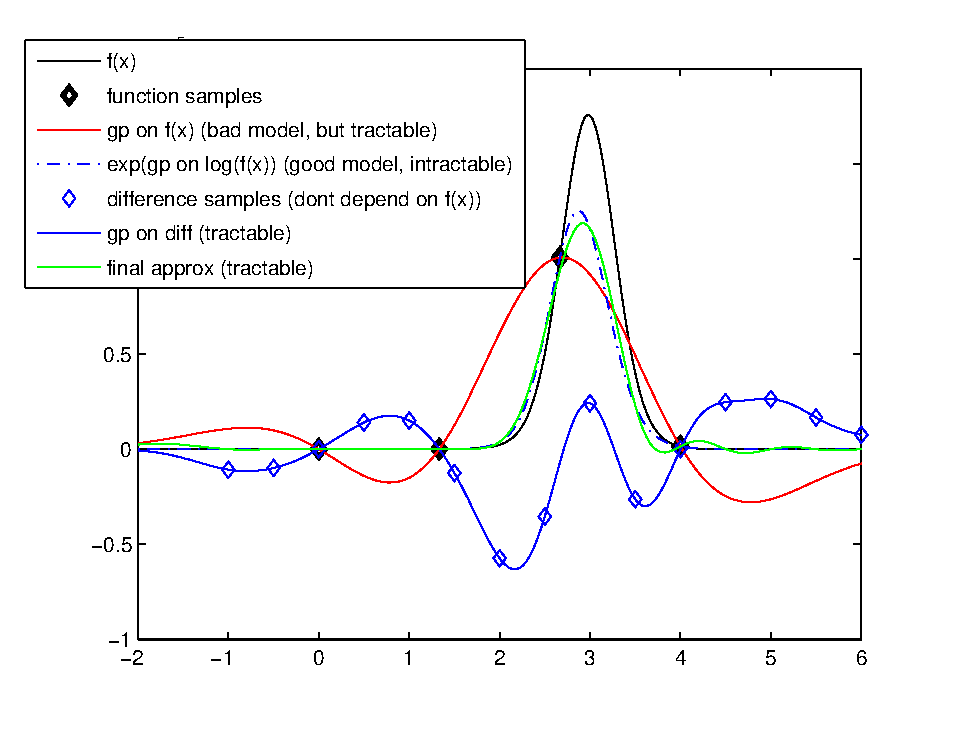
\includegraphics[width=0.48\textwidth]{figures/log_gp_diff.eps}
\caption{An illustration of model-based integration, or Bayesian Quadrature.  We compute the expected are underneath Gaussian process posterior, conditioned on sampled values of the true likelihood function.  Obtaining samples about uncertain regions allows us to reduce our uncertainty about the area under the function.  }
\label{fig:model_based}
\end{figure}

Using a model-based approach, the issue of convergence is solved naturally:  Our posterior variance over $Z$ indicates our remaining uncertainty about the quantity we care about.  This statistic is typically only reliable if we are able to integrate over all unknown quantities.  This is typically intractable, however by approximately integrating out lengthscales in section ?? we go some ways towards fixing this problem.  The results in section ?? indicate that our posterior variance is reasonably well-calibrated.

Having a reliable indicator that our estimate has converged to the truth is vital. [We need to stress this more in the intro and conclusion]

\section{Gaussian Processes}
Gaussian processes (\gp s) offer a powerful method to perform Bayesian inference about functions \citep{GPsBook}. A \gpb is defined as a distribution over the functions $f: \Phi \rightarrow \mathbb{R}$ such that the distribution over the possible function values on any finite subset of $\Phi$ is multivariate Gaussian.  For a function $f(\lfv)$, the prior distribution over its values $\vf$ on a subset $\vlfv \subset \Phi$ are completely specified by a mean vector $\vmu$ and covariance matrix $K$
\begin{align*}%\label{eq:GPDefn}
\textstyle
 &\p{\vf}{I} \deq \N{\vf}{\vmu_{f}}{K_{f}}\\
 &\deq\frac{1}{\sqrt{\det{2\pi K_{f}}}}\,\exp \big(-\frac{1}{2}\,(\vf-\vmu_{f})\tra\,K_{f}\inv\,(\vf-\vmu_{f})\big),
\end{align*}
where $I$, the \emph{context}, forms the background knowledge upon which all our probabilities are conditioned. Its ubqiuity leads us to henceforth drop it from explicit representation for notational convenience. 
The context, $I$, includes prior knowledge of both the mean and covariance functions, which generate $\vmu_{f}$ and $K_{f}$ respectively. 
The prior mean function is chosen as appropriate for the problem at hand (often a constant), and the covariance function is chosen to reflect any prior knowledge about the
structure of the function of interest, for example periodicity or differentiability. In this paper, we'll use Gaussian covariance functions,
\begin{align} \label{eq:Gaussian_cov_fn}
% K(\vlfv,\vlfv') & \deq \prod_{e=1}^{E} K_e\big(\phi\pha_e,\phi_e'\big)\\
\textstyle
K_{f}(\lfv_1,\lfv_2)& \deq h_f^2\,\N{\lfv_1}{\lfv_2}{w_{f}}.
\end{align} 
Here $h_f$ specifies the output scale (`height') over $f$, while $w_f$ defines a (squared) input scale (`width') over $\lfv$. Note that if $\lfv$ a function over multi-dimensional inputs, $w_f$ is a covariance matrix. For the remainder of the paper, we'll take $w_f$ as diagonal. 


Let us assume we have observations $(\vlfv_s,\vf_s)$ and are interested in making predictions about the function valus $f_\star$ at input $\lfv_\star$. We will assume that knowledge of function inputs such as $\vlfv_s$ and $\lfv_\star$ is incorporated into $I$ (and will hence usually be hidden). With this information, we have the predictive equations
$$
\pskinny{f\st}{\vf_s} = 
\bN{f\st}
{\meancond{f}{\vlfv_\star}{s}}
{\covcond{f}{\vlfv_\star}{s}}\,,
$$
where we have, for the mean $\novmean{a}{b}\deq \int a\,\pskinny{a}{b} \ud
a$ and variance $\novcov{a}{b}\deq \int
\big(a-\novmean{a}{b}\big)^2\,\pskinny{a}{b} \ud a$,
\begin{align} 
\textstyle
&\meancond{f}{\lfv_\star}{s}
\deq \mean{f_\star}{\vf_s}
\nonumber\\
&= \mu_{f}(\lfv_\star) + 
K_{f}(\lfv_\star,\vlfv_s)
K_{f}(\vlfv_s,\vlfv_s)\inv
\bigl(\vf_s-{\mu}_{f}(\vlfv_s)\bigr) \label{eq:GPMean}
\\
&\covcond{f}{\lfv_\star}{s}
\deq {\cov{f_\star}{\vf_s}} 
\nonumber\\
&= K_{f}(\lfv_\star,\lfv_\star) - 
K_{f}(\lfv_\star,\vlfv_s)
K_{f}(\vlfv_s,\vlfv_s)\inv
K_{f}(\vlfv_s,\lfv_\star)\,. \nonumber%\label{eq:GPCov}
\end{align} 

\section{Bayesian Quadrature} \label{sec:BQ}

% Note that maximum likelihood is also subject to issues. $\p{D}{\lfv,I}$, how come (known) $I$ is on the right and (known) $D$ is on the left? 

\emph{Bayesian quadrature} \citep{BZHermiteQuadrature,BZMonteCarlo} is a means of performing Bayesian inference about the value of a potentially nonanalytic integral 
\begin{equation} \label{eq:intyf}
 \inty{f} \deq \int f(\lfv)\,\po{\lfv}\,\ud\lfv\,.
\end{equation}
%Note that we use a condensed notation; this and all integrals to follow are definite integrals over the entire domain of interest.
We'll assume we are integrating with respect to a Gaussian prior
\begin{align}\label{eq:phiprior}
\textstyle
 \po{\lfv} & \deq \N{\lfv}{\nu_{\lfv}}{\lambda_{\lfv}} \,,
\end{align}
although other convenient forms, or, if necessary, the use of an importance re-weighting trick, allow any other integral to be approximated \citep{OsborneAnon}. If $\lfv$ is a vector, $\nu_{\lfv}$ is a  vector of identical size, and $\lambda_{\lfv}$ an appropriate covariance matrix.

%\textcolor{red}{[I'm hoping to re-write the next two paragraphs; it's way too indirect, and I think the philosophical foundations of MCMC are a poor avenue of attack]}
Quadrature involves evaluating $f(\lfv)$ at a vector of sample points $\vlfv_s$, giving $\vf\pha_s\deq f(\vlfv_s)$. Of course, this evaluation is often a computationally expensive operation. The resultant sparsity of our samples introduces uncertainty about the function $f$ between them, and hence uncertainty about the integral $\inty{f}$.

%As ever in the face of uncertainty, we address the estimation of the value of our integral as a problem of Bayesian inference \citep{BZNumericalAnalysis}. 

%In considering any problem of inference, we need to be clear about both what information we have and which uncertain variables we are interested in. In our case, both the values $f(\vlfv_s)$ and their locations $\vlfv_s$ represent valuable pieces of knowledge. As discussed by \citet{MCUnsound}, traditional Monte Carlo, which approximates as
%\begin{equation} \label{eq:MC_integral_estimate}
%\inty{f} \simeq \frac{1}{\card{s}} \sum_{i=1}^{\card{s}} f(\lfv_i)\,,
%\end{equation}
%effectively ignores the information content of $\vlfv_s$, leading to unsatisfactory behaviour.
%\footnote{  For example, imagine that we had $\card{s}=3$, and $\lfv_1 = \lfv_2$. In this case, the identical value $q(\lfv_1)= q(\lfv_2)$ will receive $\nicefrac{2}{3}$ of the weight, whereas the equally useful $q(\lfv_3)$ will receive only $\nicefrac{1}{3}$. \textcolor{red}{I'm not crazy about this argument, since the weightings are also incorporating information about the prior...} }

We choose for $f$ a \gpb prior with mean $\mu_f$ and the Gaussian covariance function \eqref{eq:Gaussian_cov_fn}. Here the scales $h_f$ and $w_f$ are \emph{quadrature hyperparameters}, hyperparameters that specify the  \gpb used for Bayesian quadrature. These scales, and the others that follow, will be taken as given and incorporated into the (hidden) context $I$.

% Many more of these will be implicitly introduced in the coming sections; we'll take this as given and incorporate them into the (hidden) context $I$. 
% Note that it will later become apparent that our inference for $\inty{f}$ is independent of the $h_f$ quadrature hyperparameter.

Note that variables over which we have a multivariate Gaussian distribution are jointly Gaussian distributed with any affine transformations of those variables. Because integration is affine, we can hence use our computed samples $\vf_s$ to perform analytic Gaussian process inference about the value of integrals over $f(\lfv)$, such as $\inty{f}$. Our mean estimate for $\inty{f}$ given $\vf_s$ is
%
\begin{align} \label{eq:mean_inty_f}
\mean{\inty{f}}{\vf_s}
& 
=\iint \inty{f}\,\p{\inty{f}}{f}\p{f}{\vf_s} \ud \inty{f} \,\ud f                                                                                                                                                               \nonumber\\
&
 =\iint \inty{f}\,\dd{\inty{f}}{\int f(\lfv)\,\po{\lfv}\,\ud\lfv}
\nonumber\\
&\hspace{2.5cm}
\N{f}{\meancondfn{f}{s}}{\covcondfn{f}{s}} \ud \inty{f} \,\ud f \nonumber\\
&
 = \int \meancondfn{f}{s}(\lfv)\,\po{\lfv}\,\ud\lfv\nonumber\\
&
 = 
%\N{\inty{f}}
\mu_f + \ntT{s}{f}\, \dtt{s}{f}
%{\varpi_{f}-\ntT{s}{f} K_{f}(\vlfv_s,\vlfv_s)\inv \nt{s}{f}}
\,,
\end{align}
where for $\lfv_i \in \vlfv_s$,
\begin{align*}
\fnt{\lfv_i}{f} & \deq \!\int K_f(\lfv_i,\lfv)\po{\lfv}\ud\lfv
 = h_f^2\,\N{\lfv_i}{\nu_{\lfv}}{\lambda_{\lfv}+w_{f}}\\
%\intertext{and}
\dtt{s}{f} & \deq K_{f}\bigl(\vlfv_s,\vlfv_s\bigr)\inv (\vf_s-{\mu}_{f})\,.
\end{align*}
%
%Note that the form of our `best estimate' for $\inty{f}$, \eqref{eq:mean_inty_f}, is an affine combination of the samples $\vf_s$, just as for traditional quadrature or Monte Carlo techniques. 
% Indeed, if $\mu_f$ is taken as the mean of $\vf_s$ (as is usual for \gpb inference), the second term in \eqref{eq:mean_inty_f} can be viewed as a correction factor to the Monte Carlo estimate \eqref{eq:MC_integral_estimate}. \textcolor{red}{[Since we're using a different sampling strategy than MCMC in this paper, I think the preceeding statement is kind of misleading / confusing...]}
% \sout{Note also that $h_f$ represents a simple multiplicative factor to both $\ntT{s}{f}$ and $K_{f}\bigl(\vlfv_s,\vlfv_s\bigr)$, and as such cancels out of \eqref{eq:mean_inty_f}.} 
%
In the following three sections, we will expand upon the improvements this paper introduces in the use of Bayesian Quadrature for computing model evidences.

\section{Modeling Likelihood Functions}

We wish to evaluate the evidence $\inty{\lfn} = \int \lfn(\lfv) p(\lfv) \ud\lfv$, an integral over non-negative likelihoods, $\lfn(\lfv)$, whose arguments are the parameters of the relevant model.


\begin{figure}
\centering
%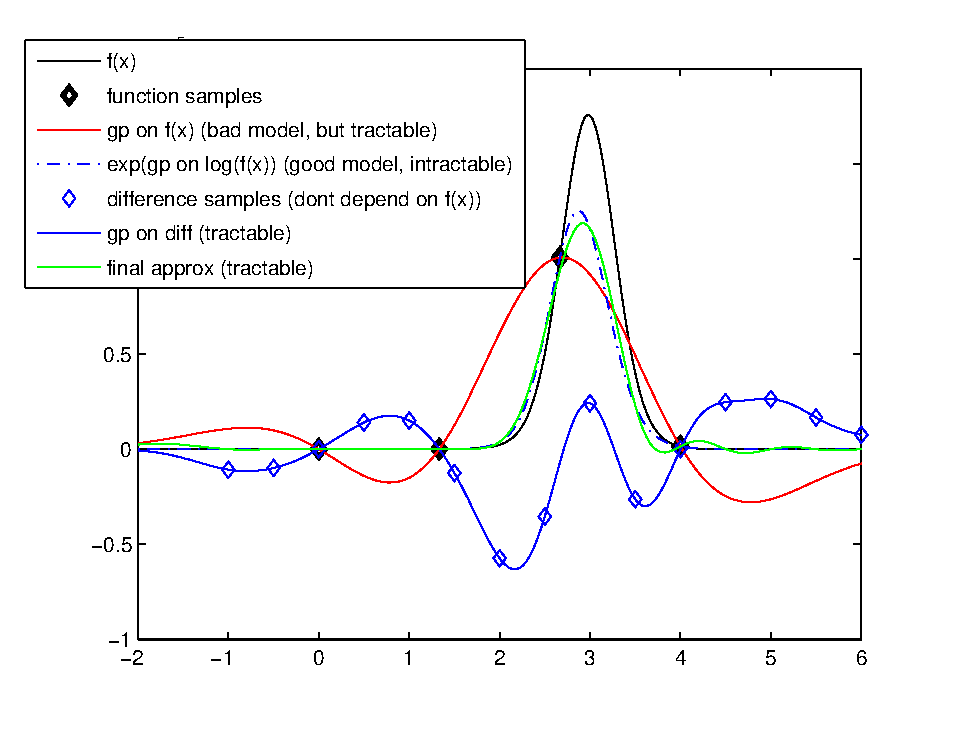
\includegraphics[width=0.48\textwidth]{figures/log_gp_diff.eps}
\caption{The lengthscale of a GP fitted to the log-likelihood function will typically be much longer than that of a GP fit to the likelihood function.  A GP with a long lengthscale will generalize better to distant parts of the function, and will have a posterior more concentrated around the true evidence. }
\label{fig:log_is_better}
\end{figure}

Assigning a standard \gpb prior to $\lfn(\lfv)$ would ignore our prior information about the range and non-negativity of $\lfn(\lfv)$, leading to pathologies such as a negative evidence (as observed in \citet{BZMonteCarlo}).  A much better prior would be a \gpb prior on $\log(\lfn(x))$.  However, the integral under the exp of a \gpb is intractable.  In this section, we apply the approximate inference method of \citep{BQR} to tractably integrate under a log-\gpb prior\footnote{In practice, we use the transform 
$\log\left(\nicefrac{\lfn(\lfv)}{\gamma} + 1\right)$
where $\gamma = (e-1)^{-1}$.  This give better resolution of some numerical issues, and allows us to assume the transformed quantity has zero mean. For the sake of simplicity, we omit this detail in the following derivations.}.

\begin{figure}
\centering
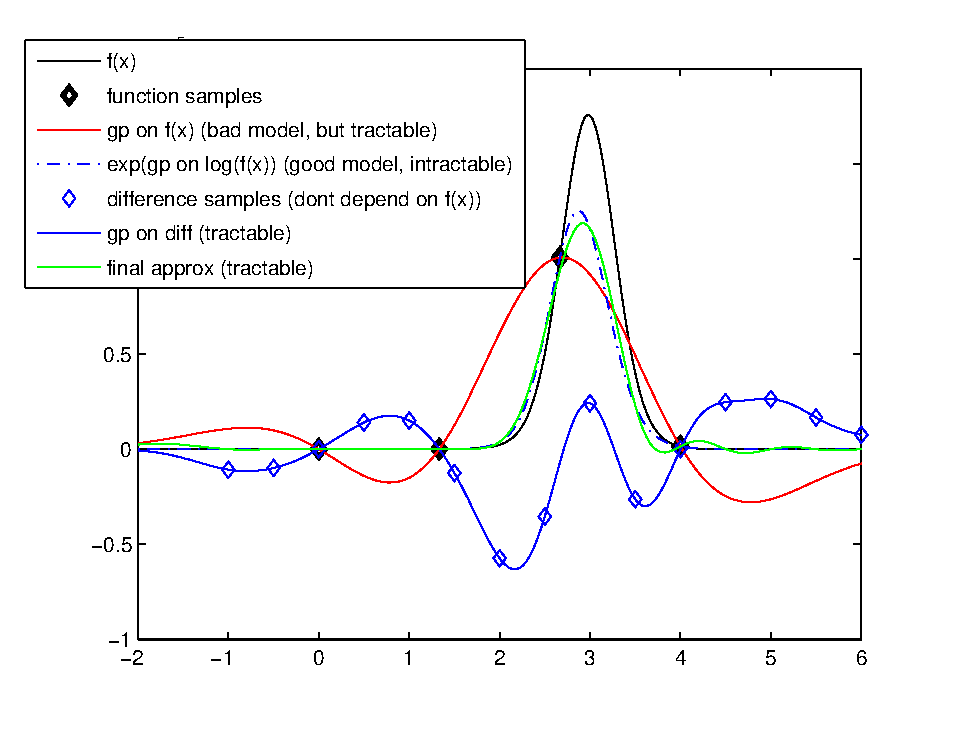
\includegraphics[width=0.48\textwidth]{figures/log_gp_diff.eps}
\caption{An illustration of our method of finding the integral under the exp of a Gaussian process. For all \gp s, we plot only the relevant posterior means.}
\label{fig:integrate_hypers}
\end{figure}

%Firstly, we define the transformation
%\begin{align*}

% \intertext{and its inverse}
% t\inv\bigl(\tr(\lfv)\bigr) & \deq \gamma \bigl(\exp \tr(\lfv)-1\bigr)
%\end{align*}
% and their inverses
% $$
% t_q\inv\bigl(\tq(\lfv)\bigr) \deq \gamma\bigl(\eta+\exp \tq(\lfv)\bigr)
% \qquad \text{and} \qquad
% t_q\inv\bigl(\tq(\lfv)\bigr) \deq \gamma\bigl(\eta+\exp \tq(\lfv)\bigr)\,,
% $$
%(which has well-defined inverse $t\inv$) where 
%$
% \gamma \deq 100\, \max(\vr_s)
%$
%is a constant introduced for superior numerical accuracy.
%
%We now assign \gpb priors to the functions
%\begin{align*}
% \tr & \deq  t(r)
%\end{align*}
% We assume that far away from our existing observations,
% the means for $q$ and $r$ are equal to a value suitably close to
% zero, and hence take a corresponding zero prior mean for the \gp s over $\tq$ and $\tr$. 
%with Gaussian
%covariances of the form \eqref{eq:Gaussian_cov_fn}.
%the minimum of the existing observations.
%These choices of prior distribution are motivated by the fact that
%$l$ is strictly positive and possesses a large dynamic
%range. 
%
%
\begin{multline}\label{eq:minty_l}
\mean{\inty{\lfn}}{\vr_s}
% & 
% =\iint \inty{l}\,\p{\inty{l}}{l}\p{l}{\vl_s} \ud \inty{l} \,\ud l                                                                                                                                                               \nonumber\\
% &
 =\int \Bigl( \int \exp\bigl(\tr(\lfv)\bigr)\lfn(\lfv)\po{\lfv}\,\ud\lfv\Bigr)\\
\N{\tr}{\meancondfn{\tr}{s}}{\covcondfn{\tr}{s}} \ud \tr
\end{multline}

Here the exponential ruins the linearity that yielded the analyticity in section \ref{sec:BQ}. To combat this, we perform inference for $\inty{\lfn}$ directly as a functional of $\tr$.
%
\begin{align*}
 \psi[\tr] \deq \inty{\lfn} & = \int \exp \bigl( \tr(\lfv)\bigr) p(\lfv) \ud \lfv\\
  						    & = \int \lfn(\lfv) p(\lfv) \ud \lfv\\
\pderiv{}{\tr(\lfv)}\psi[\tr] & = \exp \bigl( \tr(\lfv)\bigr) p(\lfv)  = \lfn(\lfv) p(\lfv) 
\end{align*}

We now make a \emph{linearisation} approximation\footnote{Note that this linearisation is equivalent to taking another \gpb for $\psi$. with the affine covariance
\begin{equation*}
 K_\psi(\tr,\tr')
% \deq 
%  K_\psi\bigl((\tvq\pha_c,\tvr\pha_c),(\tvq'_c,\tvr'_c)\bigr)
\deq
\int\tr(\lfv) \tr'(\lfv) \ud \lfv
+ \omega^2\,.
\end{equation*}
} 
for $\psi$, forcing $\psi$ to be, as desired, affine in $\tr$. 
Note that \eqref{eq:minty_l} consists of the product of $\psi[\tr]$ and a \gpb for $\tr$; the latter, due to the light tails of the Gaussian, effectively permits only a small range of $\tr$ functions. Over this narrow region, it is reasonable to assume that $\psi[\tr]$ does not vary too dramatically, and can be approximated as linear. 

Before proceeding, we introduce a separate \gpb model over $\lfn$, the non-log space.  Then $m_{\lfn|s}$ is the \gpb conditional mean (as per \eqref{eq:GPMean}) for $\lfn$ given observations $\lfn(\vlfv_s)$. For this \gpb (over the non-log space), we take zero prior means and Gaussian
covariances of the form \eqref{eq:Gaussian_cov_fn}. 

We perform the linearisation of $\psi[\tr]$ around the point defined by $\tr_0 \deq \log (m_{\lfn|s})$. We make the definitions 
$\psi_0 \deq \psi[\tr_0]$, $\pderiv{\psi_0}{\tr(\lfv)} \deq \pderiv{\psi}{\tr(\lfv)}[\tr_0]$, giving us the convenient mean
\begin{multline}\label{eq:linearisation}
\novmean{\psi[\tr]}{\psi_0,\pderiv{\psi_0}{\tq(\lfv)}} 
= \psi_0+\\
\int \pderiv{\psi_0}{\tr(\lfv)}\bigl(\tr(\lfv)-\tr_0(\lfv)\bigr)\ud\lfv\,.
\end{multline}

% Our linearisation corresponds to giving our \gpb over $\psi$ observations
% at $\tr_0= \log (m_{r|s})$ of both the functional itself,
That is, we can now write
\begin{align*}
\psi_0 & = \psi[\tr_0]
= 
{\mean{\inty{\lfn}}{\vr_s}}
\intertext{along with the functional derivative}
\pderiv{\psi_0}{\tr(\lfv)} & = \pderiv{\psi}{\tr(\lfv)}[\tr_0]
 = \mean{\lfn(\lfv)}{\vr_s}\,\po{\lfv}
\nonumber
\end{align*}
Note that $\psi_0$ and its functional derivatives are analytic; our choice of $\tr_0$ permitted us to resolve the necessary integrals.

We now define
\begin{align*}
\Delta & \deq m_{\tr |s} - \log(m_{r|s}) = m_{\tr |s}  - \tr_0 \,,
\end{align*}
%\textcolor{red}{[You know, until I did the notation change, I never understood that $\Delta$ was defined on the logs, not on the untransformed quantities.]} 
the difference between the \gpb means over our log-transformed quantities and the transformed \gpb means over original quantities. 
%\textcolor{red}{[I'd like to insert here my figure 2]}. 
%we have
%\begin{align}\label{eq:mt_sim_tm}
%\Delta \simeq 0\,,
%\end{align}
%\textcolor{red}{[I found this statement confusing, it looks like we're planning to ignore $\Delta$ instead of giving it a full treatment.]}
We expect $\Delta(\lfv)$ to be everywhere small relative to the magnitude of $\tr(\phi)$ (see Figure \ref{fig:integrate_hypers}. This implies that
 $\tr_0$ is close to the peaks of our Gaussian over $\tr$, rendering our linearisation appropriate. 

For future notational convenience, we assume that if we condition on $\psi_0$, we will condition on its functional derivatives. This allows us to write our mean for  $\inty{\lfn}$
%
\begin{align}
& \mean{\inty{\lfn}}{\psi_0,\tvr_s} \nonumber\\
& \deq \int \mean{\psi[\tr]}{\psi_0,\tr}
\p{\tr}{\tvr_s}\, \ud \tr 
\nonumber\\
& = \mean{\psi[m_{\tr|s}]}{\psi_0,m_{\tr|s}} \nonumber\\
& = \mean{\inty{\lfn}}{\vr_s} + \iint \mean{\lfn(\lfv)}{\vr_s}\,
\Delta(\lfv)\,\po{\lfv}\ud\lfv
\label{eq:mean_ev1}
\end{align}

As with any linearisation approximation, \eqref{eq:mean_ev1} gives the value at the selected point $\tr_0$, plus a correction factor modelling the influence of the first derivatives. This correction factor, 
$\int \mean{\lfn(\lfv)}{\vr_s}\,
\Delta(\lfv)\,\po{\lfv}\ud\lfv$,
contains a further non-analytic integral, due to the $\tr_0$ term within $\Delta$. As such, we perform another stage of Bayesian quadrature by treating $\Delta$ as an unknown function of $\lfv$.


For this function we take Gaussian process priors with zero prior mean and Gaussian covariance \eqref{eq:Gaussian_cov_fn}. We must now choose sample points $\vlfv_c$ at which to evaluate our $\Delta$ function. 
Note that we do not need to evaluate $\lfn(\lfv_c)$ in order to compute $\Delta(\lfv_c)$.
% Unfortunately, it is impractical to resolve this decision problem in the same manner as the selection of $\vlfvS$, our ultimate goal (a topic that receives our full attention in Section \ref{sec:SBQ})).
$\vlfv_c$ should firstly include $\vlfv_s$, at which points we know that $\delta$ is equal to zero. Following \cite{BQR}, we select the remainder of $\vlfv_c$  as the  vertices of a Voronoi diagram \citep{okabe1997locational}, where we expect $\delta$ to be extremised. 

Given these samples, we can now marginalise \eqref{eq:mean_ev1} over $\Delta$ to give
\begin{align}
 \mean{\inty{\lfn}}{\psi_0,\tvr_s,\Delta_c} =
\mean{\inty{\lfn}}{\vr_s} + C\,,
\label{eq:mean_ev2}
\end{align}
where the correction factor is
\begin{align*}
 C \deq \mean{\inty{\lfn \Delta}}{\vr_s, \Delta_c}\,.
\end{align*}
As $\Delta$ is small, we expect $C$ to also be small.


\section{Sampling for Bayesian Quadrature}

We aim to select samples $\lfv_s$ so as to minimise the \textit{expected} uncertainty in the evidence after seeing our next sample.\footnote{We also expect such samples to be useful not just for estimating the evidence, but also for any other related expectations, such as would be required to perform prediction using the model.}
Surprisingly, the posterior variance of a GP model with fixed hyperparameters does not depend on the function values at sampled locations all all; only the location of those samples matters. Hence active learning is pointless, and the optimal sampling design can be found in advance \cite{minka2000dqr}.

However, because we place our GP model on the log-likelihood, our variance depends crucially on the values of the log-likelihoods observed. 

\begin{figure}
\centering
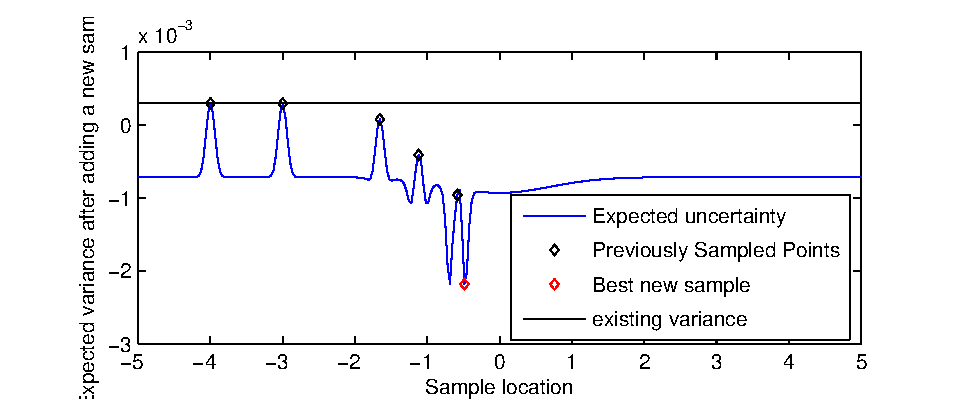
\includegraphics[width=0.48\textwidth]{figures/eue.eps}
\caption{An example the expected uncertainty in the evidence after observing the likelihood function at that location.}
\label{fig:eue}
\end{figure}

\begin{figure}
\centering
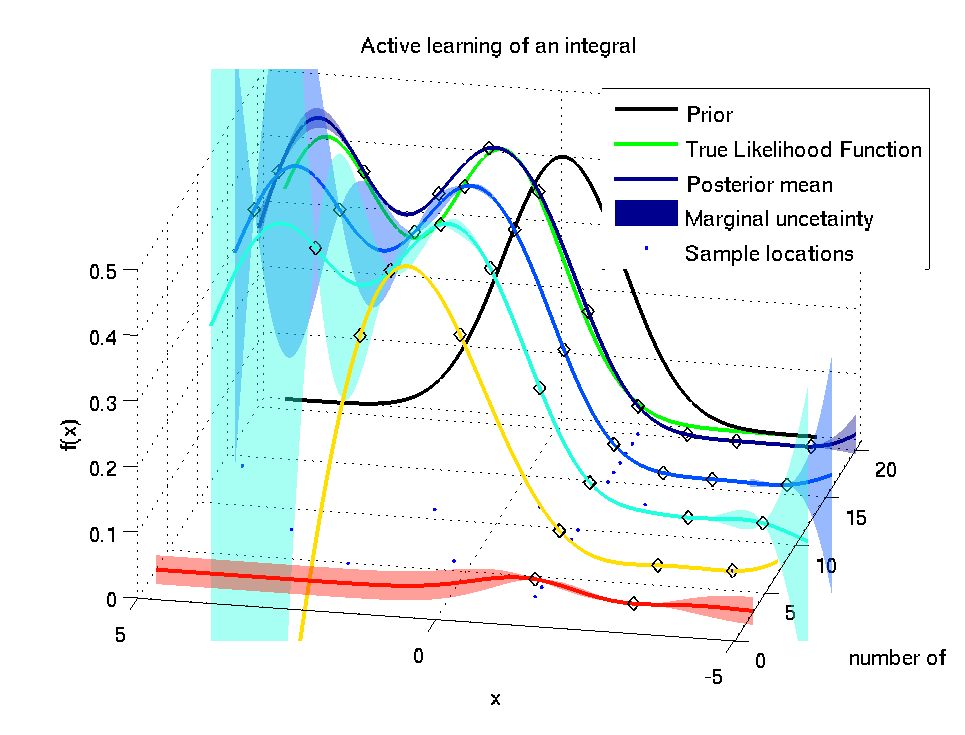
\includegraphics[width=0.48\textwidth]{figures/active_learning.eps}
\caption{An example of the posterior over likelihood functions converging as new samples are selected.}
\label{fig:active_learning}
\end{figure}

The variance in the evidence is
\begin{align*}
& \cov{\inty{\lfn}}{\psi_0,\tvr_s,\Delta_c}\\ 
& = \int \psi^2 \delta{\psi - \mean{\inty{\lfn}}{\psi_0,\tvr_s,\Delta_c}
\p{\inty{\lfn}}{\tvr_s} \ud\inty{\lfn}\\
& - \mean{\inty{\lfn}}{\psi_0,\tvr_s,\Delta_c}^2\,.
\end{align*}
To resolve the first term, define a new functional
\begin{align*}
 \chi[\tr] \deq \inty{\lfn}^2 & = \gamma^2\bigl(\int  \exp \tr(\lfv) p(\lfv) \ud \lfv-1\bigr)^2\\
\pderiv{}{\tr(\lfv)}\chi[\tr] & = 2\gamma \exp \tr(\lfv) p(\lfv) \bigl(\int  \exp \tr(\lfv) p(\lfv) \ud \lfv-1\bigr)
\end{align*}
which we again linearise around $\tr_0$. Hence, as per the above
\begin{align*}
& \cov{\inty{\lfn}}{\chi_0,\psi_0,\tvr_{s}} = \mean{\inty{\lfn}^2}{\chi_0,\tvr_s} - \mean{\inty{\lfn}}{\psi_0,\tvr_s}^2
% & =  (\mean{\inty{\lfn}}{\vr_s})^2 \\
% & \qquad + 2\mean{\inty{\lfn}}{\vr_s}
% \bigl(\mean{\inty{\lfn \Delta}}{\vr_s} + \gamma\, \mean{\inty{\Delta}}{\vr_s}\bigr)
% \\
% & \qquad - \bigl(
% \mean{\inty{\lfn}}{\vr_s} + \mean{\inty{\lfn \Delta}}{\vr_s} + \gamma\, \mean{\inty{ \Delta}}{\vr_s}
% \bigr)^2
% & = \mean{\inty{\lfn}}{\vr_s}
% \bigl(\mean{\inty{\lfn \Delta}}{\vr_s} + \gamma\, \mean{\inty{\Delta}}{\vr_s}\bigr)
% \\
% & \qquad - \bigl( \mean{\inty{\lfn \Delta}}{\vr_s} + \gamma\, \mean{\inty{ \Delta}}{\vr_s}
% \bigr)^2
% \,.
\end{align*}
where
\begin{align*}
&\mean{\inty{\lfn}^2}{\chi_0,\tvr_s} \\
& = \mean{\chi[\tr]}{\chi_0,m_{\tr|s}} \\
& = (\mean{\inty{\lfn}}{\vr_s})^2 \\
& \hspace{1cm} + 2\mean{\inty{\lfn}}{\vr_s}
\bigl(\mean{\inty{\lfn \Delta}}{\vr_s} + \gamma\, \mean{\inty{\Delta}}{\vr_s}\bigr)
\end{align*}


Consider adding a new sample at $\lfv_a$. The expected variance in our evidence after doing so is
\begin{align}
& \bigl\langle \cov{\inty{\lfn}}{\chi_0,\psi_0,\tvr_{s,a}}\mid \chi_0,\psi_0,\tvr_{s}\bigr\rangle\nonumber\\
& = \mean{\inty{\lfn}^2}{\chi_0,\tvr_s}  - 
\int\mean{\inty{\lfn}}{\psi_0,\tvr_{a,s}}^2\p{\tr_a}{\tvr_s}\ud\tr_a\,.\label{eqn:exp_var}
\end{align}
The first term is independent of the selection of $\lfv_a$ and hence can be safely ignored. Noting that $\int \exp(c\, \tr_a)\, \N{\tr_a;m, \sigma^2} \ud\tr_a = \exp(c\, m + \nicefrac{1}{2}\, c^2 \sigma^2)$, the second term can be resolved analytically for any trial $\lfv_a$ (we omit the laborious details of doing so). With this expression, we now select the $\lfv_a$ that minimises the second term using a numerical optimisation technique. 

\section{Marginalising quadrature hyperparameters}

Hitherto, we have taken the maximum likelihood values $m_\theta$ for the quadrature hyperparameters $\theta$ of the quadrature-\gpb used to model the integrand. Once we have very many samples, this approximation seems reasonable: with lots of data, we can be almost certain about the values of the quadrature hyperparameters. However, in the process of taking samples, we'd like to acknowledge the influence new samples may have on our beliefs about the quadrature-hyperparameters. We'd expect this would further promote exploration, particularly early on, so as to firm up our beliefs about the quadrature-hyperparameters. The quadrature-hyperparameters of most interest are the input scales $w_r$; these hyperparameters can have a very dramatic influence on our fit to a function.

\begin{figure}
\centering
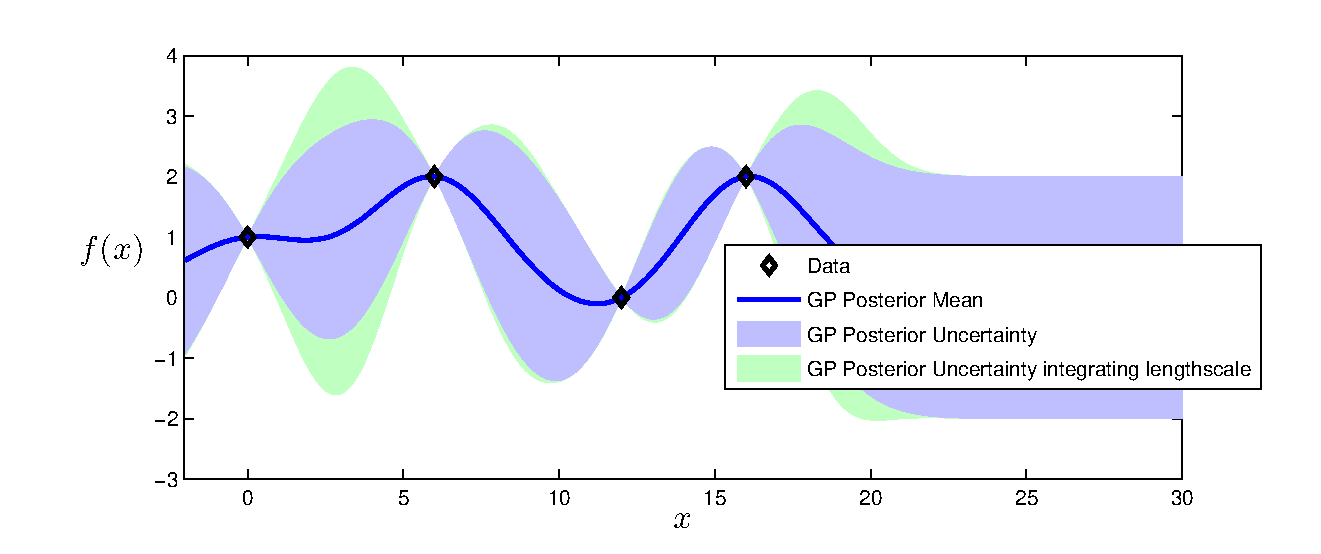
\includegraphics[width=0.48\textwidth]{figures/integrate_lengthscales.eps}
\caption{A demo of the effect of integrating hyperparameters on the marginal posterior variance.}
\label{fig:integrate_hypers}
\end{figure}

Unfortunately, the dependence of our predictions upon these input scales is complex, ruling out analytic results. However, any approximation we make is likely to improve upon our existing assumption that the posterior for all quadrature-hyperparameters is a delta function! Our approach will be to assume that
\begin{itemize}
 \item that the posterior for $\theta$ is Gaussian with mean equal to the maximum likelihood value $m_\theta$, essentially assuming that our prior is very broad. 
\item The Gaussian's covariance matrix $C_\theta$ is taken as diagonal. For quadrature hyperparameters other than the input scales, we take the appropriate diagonal elements as infinitesimally small, such that our posterior for these parameters is a delta function. For the the diagonal elements corresponding to $w_r$, we use [To be determined]
%the squared input scales $w_s$ of another \gp, fitted to the likelihood $s(w_r)$ of the input scales $w_r$. \textcolor{red}{[Neat idea, but I can think of simple examples where the lengthscale is short but the mass is spread out; it seems to me that it'd be better to first fit a GP, then fit a Gaussian to the \gpb posterior.]}
\item that our predictions for $\tr_a$ have a mean which is linear in $w_r$ around the maximum likelihood values, and a variance which is essentially constant.  
\end{itemize}
 
The implication of these assumptions is that the posterior mean over our functions remains the same.
 % David sez: I moved this to the appendix.
%With these assumptions, we have
%\begin{align*}
%& \mean{\inty{\lfn}}{\psi_0,\tvr_s} \\
%& \deq \iint \mean{\psi[\tr]}{\psi_0,\tr}
%\p{\tr}{\tvr_s, \theta}\, \p{\theta}{\tvr_s}\ud \tr\,\ud \theta\\
%& = \iint \mean{\psi[\tr]}{\psi_0,\tr} \N{\tr}{m_{\tr|s,\theta}}{C_{\tr|s,\theta}}
%\\
%& \hspace{5cm}\N{\theta}{m_\theta}{C_\theta}\ud \tr\,\ud \theta
%\\
%& \simeq \iint \mean{\psi[\tr]}{\psi_0,\tr} 
%\\
%& \hspace{2cm}\N{\tr}
%{m_{\tr|s,m_\theta}+\pderiv{m_{\tr|s,\theta}}{\theta}(\theta-m_\theta)}
%{C_{\tr|s,m_\theta}}
%\\
%& \hspace{4cm}
%\N{\theta}{m_\theta}{C_\theta}\ud \tr\,\ud \theta
%\\
%& = \iint \mean{\psi[\tr]}{\psi_0,\tr} \\
%& \hspace{1cm}\N{\tr}
%{m_{\tr|s,m_\theta}}
%{C_{\tr|s,m_\theta}+\pderiv{m_{\tr|s,\theta}}{\theta}C_\theta\pderiv{m\tra_{\tr|s,\theta}}{\theta}}
%\ud \tr
%\\
%& = \mean{\psi[\tr]}{\psi_0,m_{\tr|s,m_\theta}}\,,
%\end{align*}
%which is identical to \eqref{eq:mean_ev} (note that we had previously just implicitly assumed that $\theta=m_\theta$). 
However, for the expected variance after adding a sample, we have
\begin{align}\label{eqn:exp_var_wtheta}
& \bigl\langle \cov{\inty{\lfn}}{\chi_0,\psi_0,\tvr_{s,a}}\mid \chi_0,\psi_0,\tvr_{s}\bigr\rangle
\nonumber\\
& =  \mean{\chi[\tr]}{\chi_0,m_{\tr|s,m_\theta}}  - 
\int\mean{\inty{\lfn}}{\psi_0,\tvr_{a,s}}^2
\nonumber\\
& \hspace{2cm}
\times\N{\tr_a}
{\tilde{m}_a }
{\tilde{C}_a +\pderiv{\tilde{m}_a}{\theta}C_\theta\pderiv{\tilde{m}\tra_a}{\theta}}
\ud\tr_a\,.
\end{align}
where
\begin{align*}
\tilde{m}_a & \deq \mean{\tr_a}{\tvr_s,m_\theta}\\
\tilde{C}_a & \deq \cov{\tr_a}{\tvr_s,m_\theta}\,.
\end{align*}
As with \eqref{eqn:exp_var}, \eqref{eqn:exp_var_wtheta} can be evaluated analytically, and minimised to determine the optimal $\lfv_a$.
Hence our variance for $\tr_a$ has been inflated due to our consideration of the influence of hyperparameters (See Figure \ref{fig:integrate_hypers}), which we expect to promote additional exploration, as desired.

\section{Experiments}

In this section we attempt to show that our changes to the BMC algorithm improve its convergence to the truth.  We also compare against several standard MCMC methods.

\paragraph{Integrands}

We chose a set of problems which would demonstrate the strengths and weakness of the various methods we compared.

we recreated the hyperparamter integration problem from \citep{BZMonteCarlo}.

[insert table of problem names and descriptions]

\paragraph{Methods}

\begin{itemize}
\item Simple Monte Carlo (SMC)
\item Annealed Importance Sampling (AIS) - the temperature schedule was linear as in \citep{BZMonteCarlo}, and the proposal width was adjusted to attain approximately 50\% acceptance rate.  Note that this is a bit of extra 'tender loving care'.
\item Bayesian Monte Carlo (BMC) - the algorithm used in \citep{BZMonteCarlo}, in which samples were chosen from a AIS chain.
\item Sequential Bayesian Quadrature (SBQ)
\end{itemize}

\paragraph{Evaluation}

\begin{figure}
\centering
\begin{tabular}{ccc}
	\hspace{-.5cm}
	\setlength\fheight{2cm} 
	\setlength\fwidth{2cm}
	% This file was created by matlab2tikz v0.1.4.
% Copyright (c) 2008--2012, Nico Schlömer <nico.schloemer@gmail.com>
% All rights reserved.
% 
% 
% 
\begin{tikzpicture}

\begin{axis}[%
xmin=-1.5, xmax=3,
xticklabels={\empty},
ymin=0, ymax=1.4,
yticklabels={\empty},
scale only axis,
width=\fwidth,
height=\fheight,
title={easy 1d},
axis on top]
\addplot [
color=green,
solid,
line width=1.0pt
]
coordinates{
 (-1.1976176963403,0.0514783667275364)(-1.1934182615128,0.051891844954746)(-1.18921882668529,0.0523078056631128)(-1.18501939185778,0.0527262553612466)(-1.18081995703027,0.0531472004896883)(-1.17662052220276,0.0535706474199511)(-1.17242108737525,0.0539966024535588)(-1.16822165254775,0.054425071821083)(-1.16402221772024,0.0548560616811771)(-1.15982278289273,0.0552895781196099)(-1.15562334806522,0.0557256271482957)(-1.15142391323771,0.0561642147043246)(-1.14722447841021,0.0566053466489896)(-1.1430250435827,0.0570490287668125)(-1.13882560875519,0.0574952667645691)(-1.13462617392768,0.0579440662703119)(-1.13042673910017,0.0583954328323923)(-1.12622730427267,0.0588493719184813)(-1.12202786944516,0.0593058889145889)(-1.11782843461765,0.0597649891240824)(-1.11362899979014,0.0602266777667045)(-1.10942956496263,0.0606909599775892)(-1.10523013013512,0.0611578408062781)(-1.10103069530762,0.0616273252157355)(-1.09683126048011,0.0620994180813626)(-1.0926318256526,0.0625741241900118)(-1.08843239082509,0.063051448239)(-1.08423295599758,0.0635313948351219)(-1.08003352117008,0.064013968493663)(-1.07583408634257,0.0644991736374122)(-1.07163465151506,0.0649870145956747)(-1.06743521668755,0.0654774956032848)(-1.06323578186004,0.0659706207996183)(-1.05903634703254,0.0664663942276063)(-1.05483691220503,0.0669648198327481)(-1.05063747737752,0.0674659014621252)(-1.04643804255001,0.0679696428634158)(-1.0422386077225,0.0684760476839094)(-1.03803917289499,0.0689851194695229)(-1.03383973806749,0.0694968616638167)(-1.02964030323998,0.0700112776070125)(-1.02544086841247,0.0705283705350113)(-1.02124143358496,0.0710481435784136)(-1.01704199875745,0.0715705997615391)(-1.01284256392995,0.0720957420014499)(-1.00864312910244,0.0726235731069736)(-1.00444369427493,0.0731540957777279)(-1.00024425944742,0.0736873126031483)(-0.996044824619914,0.0742232260615156)(-0.991845389792406,0.0747618385189865)(-0.987645954964898,0.0753031522286264)(-0.98344652013739,0.0758471693294426)(-0.979247085309881,0.0763938918454223)(-0.975047650482373,0.0769433216845697)(-0.970848215654865,0.0774954606379487)(-0.966648780827357,0.0780503103787256)(-0.962449345999849,0.0786078724612159)(-0.958249911172341,0.0791681483199332)(-0.954050476344833,0.0797311392686408)(-0.949851041517325,0.080296846499407)(-0.945651606689816,0.0808652710816625)(-0.941452171862308,0.0814364139612619)(-0.9372527370348,0.0820102759595477)(-0.933053302207292,0.082586857772418)(-0.928853867379784,0.0831661599693982)(-0.924654432552276,0.0837481829927153)(-0.920454997724768,0.0843329271563767)(-0.91625556289726,0.0849203926452532)(-0.912056128069752,0.0855105795141644)(-0.907856693242243,0.0861034876869703)(-0.903657258414735,0.0866991169556654)(-0.899457823587227,0.0872974669794781)(-0.895258388759719,0.0878985372839739)(-0.891058953932211,0.0885023272601637)(-0.886859519104703,0.0891088361636166)(-0.882660084277195,0.0897180631135772)(-0.878460649449687,0.0903300070920881)(-0.874261214622179,0.0909446669431176)(-0.87006177979467,0.0915620413716921)(-0.865862344967162,0.092182128943034)(-0.861662910139654,0.0928049280817048)(-0.857463475312146,0.0934304370707546)(-0.853264040484638,0.0940586540508756)(-0.84906460565713,0.0946895770195627)(-0.844865170829622,0.0953232038302795)(-0.840665736002114,0.0959595321916301)(-0.836466301174605,0.0965985596665375)(-0.832266866347097,0.0972402836714277)(-0.828067431519589,0.0978847014754203)(-0.823867996692081,0.0985318101995256)(-0.819668561864573,0.099181606815849)(-0.815469127037065,0.0998340881468001)(-0.811269692209557,0.100489250864311)(-0.807070257382049,0.101147091489061)(-0.802870822554541,0.101807606389705)(-0.798671387727032,0.102470791782117)(-0.794471952899524,0.103136643728629)(-0.790272518072016,0.103805158137291)(-0.786073083244508,0.104476330761127)(-0.781873648417,0.105150157197408)(-0.777674213589492,0.10582663288692)(-0.773474778761984,0.106505753113259)(-0.769275343934476,0.107187513002114)(-0.765075909106968,0.107871907520572)(-0.760876474279459,0.108558931476425)(-0.756677039451951,0.109248579517487)(-0.752477604624443,0.10994084613092)(-0.748278169796935,0.110635725642568)(-0.744078734969427,0.1113332122163)(-0.739879300141919,0.112033299853359)(-0.735679865314411,0.112735982391728)(-0.731480430486903,0.113441253505495)(-0.727280995659395,0.114149106704233)(-0.723081560831886,0.114859535332391)(-0.718882126004378,0.115572532568687)(-0.71468269117687,0.11628809142552)(-0.710483256349362,0.117006204748387)(-0.706283821521854,0.117726865215303)(-0.702084386694346,0.118450065336248)(-0.697884951866838,0.119175797452604)(-0.69368551703933,0.119904053736621)(-0.689486082211822,0.120634826190877)(-0.685286647384313,0.121368106647759)(-0.681087212556805,0.122103886768951)(-0.676887777729297,0.122842158044931)(-0.672688342901789,0.123582911794484)(-0.668488908074281,0.124326139164217)(-0.664289473246773,0.125071831128096)(-0.660090038419265,0.125819978486984)(-0.655890603591757,0.126570571868195)(-0.651691168764248,0.127323601725062)(-0.64749173393674,0.12807905833651)(-0.643292299109232,0.128836931806643)(-0.639092864281724,0.129597212064346)(-0.634893429454216,0.130359888862894)(-0.630693994626708,0.131124951779576)(-0.6264945597992,0.131892390215327)(-0.622295124971692,0.132662193394379)(-0.618095690144184,0.133434350363917)(-0.613896255316675,0.134208849993748)(-0.609696820489167,0.134985680975992)(-0.605497385661659,0.135764831824767)(-0.601297950834151,0.136546290875908)(-0.597098516006643,0.137330046286682)(-0.592899081179135,0.138116086035521)(-0.588699646351627,0.138904397921774)(-0.584500211524119,0.13969496956546)(-0.58030077669661,0.140487788407048)(-0.576101341869102,0.141282841707236)(-0.571901907041594,0.142080116546754)(-0.567702472214086,0.142879599826173)(-0.563503037386578,0.143681278265737)(-0.55930360255907,0.144485138405194)(-0.555104167731562,0.145291166603656)(-0.550904732904054,0.146099349039462)(-0.546705298076546,0.146909671710057)(-0.542505863249037,0.147722120431892)(-0.538306428421529,0.148536680840325)(-0.534106993594021,0.149353338389548)(-0.529907558766513,0.150172078352523)(-0.525708123939005,0.15099288582093)(-0.521508689111497,0.151815745705134)(-0.517309254283989,0.152640642734166)(-0.513109819456481,0.153467561455711)(-0.508910384628973,0.154296486236123)(-0.504710949801464,0.155127401260442)(-0.500511514973956,0.155960290532437)(-0.496312080146448,0.156795137874654)(-0.49211264531894,0.157631926928486)(-0.487913210491432,0.158470641154253)(-0.483713775663924,0.159311263831301)(-0.479514340836416,0.160153778058113)(-0.475314906008908,0.160998166752437)(-0.4711154711814,0.161844412651428)(-0.466916036353891,0.162692498311807)(-0.462716601526383,0.163542406110031)(-0.458517166698875,0.164394118242487)(-0.454317731871367,0.16524761672569)(-0.450118297043859,0.166102883396505)(-0.445918862216351,0.166959899912384)(-0.441719427388843,0.167818647751615)(-0.437519992561335,0.168679108213586)(-0.433320557733826,0.169541262419072)(-0.429121122906318,0.170405091310529)(-0.42492168807881,0.171270575652411)(-0.420722253251302,0.172137696031496)(-0.416522818423794,0.173006432857235)(-0.412323383596286,0.173876766362112)(-0.408123948768778,0.174748676602023)(-0.40392451394127,0.175622143456667)(-0.399725079113762,0.176497146629959)(-0.395525644286253,0.177373665650457)(-0.391326209458745,0.178251679871799)(-0.387126774631237,0.179131168473168)(-0.382927339803729,0.180012110459761)(-0.378727904976221,0.180894484663286)(-0.374528470148713,0.181778269742466)(-0.370329035321205,0.182663444183563)(-0.366129600493697,0.18354998630092)(-0.361930165666189,0.184437874237516)(-0.35773073083868,0.185327085965542)(-0.353531296011172,0.186217599286989)(-0.349331861183664,0.187109391834252)(-0.345132426356156,0.18800244107076)(-0.340932991528648,0.188896724291607)(-0.33673355670114,0.189792218624215)(-0.332534121873632,0.190688901029002)(-0.328334687046124,0.191586748300073)(-0.324135252218615,0.192485737065927)(-0.319935817391107,0.193385843790177)(-0.315736382563599,0.194287044772292)(-0.311536947736091,0.195189316148352)(-0.307337512908583,0.196092633891817)(-0.303138078081075,0.196996973814322)(-0.298938643253567,0.197902311566479)(-0.294739208426059,0.198808622638699)(-0.290539773598551,0.199715882362034)(-0.286340338771042,0.200624065909032)(-0.282140903943534,0.201533148294607)(-0.277941469116026,0.202443104376929)(-0.273742034288518,0.203353908858332)(-0.26954259946101,0.204265536286236)(-0.265343164633502,0.205177961054081)(-0.261143729805994,0.206091157402289)(-0.256944294978486,0.207005099419232)(-0.252744860150978,0.207919761042222)(-0.248545425323469,0.208835116058517)(-0.244345990495961,0.209751138106339)(-0.240146555668453,0.210667800675916)(-0.235947120840945,0.211585077110537)(-0.231747686013437,0.212502940607619)(-0.227548251185929,0.213421364219797)(-0.223348816358421,0.214340320856028)(-0.219149381530913,0.215259783282711)(-0.214949946703405,0.216179724124822)(-0.210750511875896,0.217100115867066)(-0.206551077048388,0.218020930855051)(-0.20235164222088,0.218942141296464)(-0.198152207393372,0.219863719262283)(-0.193952772565864,0.220785636687983)(-0.189753337738356,0.221707865374778)(-0.185553902910848,0.222630376990866)(-0.18135446808334,0.223553143072693)(-0.177155033255832,0.224476135026237)(-0.172955598428323,0.225399324128304)(-0.168756163600815,0.226322681527837)(-0.164556728773307,0.22724617824725)(-0.160357293945799,0.228169785183766)(-0.156157859118291,0.22909347311078)(-0.151958424290783,0.230017212679231)(-0.147758989463275,0.230940974418997)(-0.143559554635767,0.231864728740292)(-0.139360119808259,0.232788445935098)(-0.13516068498075,0.233712096178589)(-0.130961250153242,0.234635649530593)(-0.126761815325734,0.23555907593705)(-0.122562380498226,0.236482345231496)(-0.118362945670718,0.237405427136562)(-0.11416351084321,0.238328291265478)(-0.109964076015702,0.239250907123605)(-0.105764641188194,0.240173244109972)(-0.101565206360685,0.241095271518829)(-0.0973657715331773,0.242016958541219)(-0.0931663367056692,0.24293827426656)(-0.0889669018781609,0.243859187684241)(-0.0847674670506529,0.244779667685238)(-0.0805680322231448,0.245699683063733)(-0.0763685973956367,0.246619202518761)(-0.0721691625681284,0.247538194655858)(-0.0679697277406206,0.248456627988728)(-0.0637702929131125,0.249374470940929)(-0.0595708580856045,0.250291691847562)(-0.0553714232580962,0.25120825895698)(-0.0511719884305881,0.252124140432509)(-0.0469725536030801,0.253039304354184)(-0.042773118775572,0.253953718720491)(-0.0385736839480637,0.254867351450133)(-0.0343742491205556,0.255780170383797)(-0.0301748142930476,0.256692143285945)(-0.0259753794655393,0.257603237846605)(-0.0217759446380312,0.25851342168319)(-0.0175765098105232,0.259422662342311)(-0.0133770749830151,0.260330927301619)(-0.00917764015550682,0.261238183971649)(-0.00497820532799875,0.262144399697678)(-0.000778770500490689,0.263049541761595)(0.00342066432701738,0.263953577383786)(0.00762009915452566,0.264856473725023)(0.0118195339820337,0.265758197888372)(0.0160189688095418,0.266658716921108)(0.0202184036370501,0.26755799781664)(0.0244178384645581,0.26845600751645)(0.0286172732920662,0.269352712912043)(0.0328167081195743,0.270248080846904)(0.0370161429470826,0.271142078118467)(0.0412155777745904,0.272034671480096)(0.0454150126020985,0.272925827643075)(0.0496144474296065,0.273815513278605)(0.0538138822571148,0.274703695019818)(0.0580133170846229,0.275590339463793)(0.0622127519121309,0.276475413173583)(0.066412186739639,0.277358882680257)(0.0706116215671473,0.278240714484946)(0.0748110563946554,0.279120875060894)(0.0790104912221634,0.279999330855532)(0.0832099260496717,0.280876048292542)(0.0874093608771798,0.281750993773945)(0.0916087957046878,0.282624133682187)(0.0958082305321959,0.283495434382243)(0.100007665359704,0.284364862223714)(0.104207100187212,0.285232383542952)(0.10840653501472,0.28609796466517)(0.112605969842228,0.286961571906581)(0.116805404669737,0.287823171576527)(0.121004839497245,0.288682729979624)(0.125204274324753,0.289540213417914)(0.129403709152261,0.29039558819302)(0.133603143979769,0.291248820608306)(0.137802578807277,0.292099876971051)(0.142002013634785,0.292948723594622)(0.146201448462294,0.293795326800656)(0.150400883289801,0.294639652921245)(0.154600318117309,0.295481668301131)(0.158799752944818,0.2963213392999)(0.162999187772326,0.297158632294191)(0.167198622599834,0.297993513679897)(0.171398057427342,0.298825949874379)(0.17559749225485,0.299655907318689)(0.179796927082358,0.300483352479781)(0.183996361909866,0.301308251852745)(0.188195796737374,0.302130571963032)(0.192395231564882,0.302950279368687)(0.196594666392391,0.303767340662588)(0.200794101219899,0.304581722474682)(0.204993536047407,0.305393391474232)(0.209192970874915,0.306202314372058)(0.213392405702423,0.307008457922791)(0.217591840529931,0.307811788927116)(0.221791275357439,0.308612274234035)(0.225990710184948,0.309409880743112)(0.230190145012456,0.310204575406738)(0.234389579839964,0.310996325232384)(0.238589014667472,0.311785097284865)(0.24278844949498,0.312570858688597)(0.246987884322488,0.313353576629863)(0.251187319149996,0.314133218359073)(0.255386753977504,0.31490975119303)(0.259586188805012,0.315683142517189)(0.26378562363252,0.316453359787927)(0.267985058460029,0.317220370534802)(0.272184493287537,0.317984142362819)(0.276383928115045,0.31874464295469)(0.280583362942553,0.319501840073098)(0.284782797770061,0.320255701562961)(0.288982232597569,0.321006195353683)(0.293181667425077,0.321753289461422)(0.297381102252585,0.322496951991341)(0.301580537080093,0.323237151139866)(0.305779971907602,0.323973855196936)(0.30997940673511,0.324707032548254)(0.314178841562618,0.325436651677537)(0.318378276390126,0.32616268116876)(0.322577711217634,0.326885089708397)(0.326777146045142,0.327603846087661)(0.33097658087265,0.32831891920474)(0.335176015700159,0.329030278067029)(0.339375450527667,0.329737891793356)(0.343574885355175,0.330441729616208)(0.347774320182683,0.331141760883949)(0.351973755010191,0.331837955063037)(0.356173189837699,0.332530281740234)(0.360372624665207,0.333218710624807)(0.364572059492715,0.333903211550736)(0.368771494320223,0.334583754478902)(0.372970929147731,0.335260309499278)(0.37717036397524,0.335932846833112)(0.381369798802748,0.336601336835107)(0.385569233630256,0.337265749995586)(0.389768668457764,0.337926056942661)(0.393968103285272,0.338582228444388)(0.39816753811278,0.339234235410917)(0.402366972940288,0.339882048896638)(0.406566407767796,0.340525640102315)(0.410765842595304,0.341164980377212)(0.414965277422813,0.341800041221215)(0.419164712250321,0.342430794286948)(0.423364147077829,0.34305721138187)(0.427563581905337,0.343679264470375)(0.431763016732845,0.344296925675875)(0.435962451560353,0.344910167282883)(0.440161886387861,0.345518961739075)(0.44436132121537,0.346123281657355)(0.448560756042878,0.3467230998179)(0.452760190870386,0.347318389170201)(0.456959625697894,0.347909122835094)(0.461159060525402,0.348495274106778)(0.46535849535291,0.349076816454825)(0.469557930180418,0.349653723526175)(0.473757365007926,0.350225969147127)(0.477956799835434,0.350793527325315)(0.482156234662942,0.35135637225167)(0.486355669490451,0.351914478302377)(0.490555104317959,0.352467820040815)(0.494754539145467,0.353016372219485)(0.498953973972975,0.353560109781932)(0.503153408800483,0.354099007864647)(0.507352843627991,0.354633041798961)(0.511552278455499,0.355162187112925)(0.515751713283007,0.355686419533177)(0.519951148110515,0.356205714986796)(0.524150582938024,0.356720049603144)(0.528350017765532,0.357229399715691)(0.53254945259304,0.35773374186383)(0.536748887420548,0.358233052794677)(0.540948322248056,0.358727309464854)(0.545147757075564,0.359216489042264)(0.549347191903072,0.359700568907845)(0.55354662673058,0.36017952665731)(0.557746061558089,0.36065334010288)(0.561945496385597,0.361121987274991)(0.566144931213105,0.361585446423993)(0.570344366040613,0.36204369602183)(0.574543800868121,0.362496714763709)(0.578743235695629,0.362944481569747)(0.582942670523137,0.363386975586604)(0.587142105350645,0.363824176189104)(0.591341540178153,0.364256062981837)(0.595540975005661,0.364682615800742)(0.59974040983317,0.365103814714673)(0.603939844660678,0.365519640026957)(0.608139279488186,0.365930072276926)(0.612338714315694,0.366335092241429)(0.616538149143202,0.366734680936342)(0.62073758397071,0.367128819618044)(0.624937018798218,0.367517489784882)(0.629136453625726,0.36790067317862)(0.633335888453235,0.368278351785869)(0.637535323280743,0.368650507839497)(0.641734758108251,0.369017123820021)(0.645934192935759,0.369378182456981)(0.650133627763267,0.369733666730297)(0.654333062590775,0.370083559871607)(0.658532497418283,0.370427845365582)(0.662731932245791,0.370766506951228)(0.6669313670733,0.371099528623164)(0.671130801900808,0.371426894632881)(0.675330236728316,0.37174858948999)(0.679529671555824,0.372064597963433)(0.683729106383332,0.372374905082696)(0.68792854121084,0.372679496138981)(0.692127976038348,0.372978356686374)(0.696327410865856,0.373271472542986)(0.700526845693364,0.373558829792071)(0.704726280520872,0.373840414783132)(0.708925715348381,0.374116214132998)(0.713125150175889,0.374386214726888)(0.717324585003397,0.374650403719444)(0.721524019830905,0.374908768535756)(0.725723454658413,0.375161296872355)(0.729922889485921,0.375407976698194)(0.734122324313429,0.375648796255599)(0.738321759140937,0.375883744061202)(0.742521193968446,0.37611280890686)(0.746720628795954,0.376335979860541)(0.750920063623462,0.376553246267193)(0.75511949845097,0.376764597749597)(0.759318933278478,0.376970024209186)(0.763518368105986,0.377169515826856)(0.767717802933494,0.377363063063742)(0.771917237761002,0.377550656661983)(0.776116672588511,0.377732287645458)(0.780316107416019,0.377907947320503)(0.784515542243527,0.378077627276601)(0.788714977071035,0.378241319387059)(0.792914411898543,0.37839901580965)(0.797113846726051,0.378550708987244)(0.801313281553559,0.378696391648412)(0.805512716381067,0.378836056808003)(0.809712151208575,0.378969697767704)(0.813911586036084,0.379097308116577)(0.818111020863592,0.37921888173157)(0.8223104556911,0.379334412778006)(0.826509890518608,0.379443895710051)(0.830709325346116,0.379547325271158)(0.834908760173624,0.379644696494486)(0.839108195001132,0.3797360047033)(0.84330762982864,0.379821245511343)(0.847507064656149,0.379900414823186)(0.851706499483657,0.379973508834561)(0.855905934311165,0.380040524032661)(0.860105369138672,0.380101457196423)(0.864304803966181,0.380156305396787)(0.868504238793689,0.38020506599693)(0.872703673621197,0.380247736652474)(0.876903108448705,0.38028431531168)(0.881102543276214,0.380314800215607)(0.885301978103721,0.380339189898258)(0.88950141293123,0.380357483186692)(0.893700847758738,0.380369679201122)(0.897900282586246,0.380375777354984)(0.902099717413754,0.380375777354984)(0.906299152241262,0.380369679201122)(0.91049858706877,0.380357483186692)(0.914698021896279,0.380339189898258)(0.918897456723786,0.380314800215607)(0.923096891551295,0.38028431531168)(0.927296326378803,0.380247736652474)(0.931495761206311,0.38020506599693)(0.935695196033819,0.380156305396787)(0.939894630861327,0.380101457196423)(0.944094065688835,0.380040524032661)(0.948293500516344,0.379973508834561)(0.952492935343851,0.379900414823186)(0.956692370171359,0.379821245511343)(0.960891804998868,0.3797360047033)(0.965091239826375,0.379644696494486)(0.969290674653884,0.379547325271158)(0.973490109481392,0.379443895710051)(0.9776895443089,0.379334412778006)(0.981888979136408,0.37921888173157)(0.986088413963916,0.379097308116577)(0.990287848791424,0.378969697767704)(0.994487283618933,0.378836056808003)(0.99868671844644,0.378696391648412)(1.00288615327395,0.378550708987244)(1.00708558810146,0.37839901580965)(1.01128502292896,0.378241319387059)(1.01548445775647,0.378077627276601)(1.01968389258398,0.377907947320503)(1.02388332741149,0.377732287645458)(1.028082762239,0.377550656661983)(1.03228219706651,0.377363063063742)(1.03648163189401,0.377169515826856)(1.04068106672152,0.376970024209186)(1.04488050154903,0.376764597749597)(1.04907993637654,0.376553246267193)(1.05327937120405,0.376335979860541)(1.05747880603155,0.37611280890686)(1.06167824085906,0.375883744061202)(1.06587767568657,0.375648796255599)(1.07007711051408,0.375407976698194)(1.07427654534159,0.375161296872355)(1.07847598016909,0.374908768535756)(1.0826754149966,0.374650403719444)(1.08687484982411,0.374386214726888)(1.09107428465162,0.374116214132998)(1.09527371947913,0.373840414783132)(1.09947315430664,0.373558829792071)(1.10367258913414,0.373271472542986)(1.10787202396165,0.372978356686374)(1.11207145878916,0.372679496138981)(1.11627089361667,0.372374905082696)(1.12047032844418,0.372064597963433)(1.12466976327168,0.37174858948999)(1.12886919809919,0.371426894632881)(1.1330686329267,0.371099528623164)(1.13726806775421,0.370766506951228)(1.14146750258172,0.370427845365582)(1.14566693740922,0.370083559871607)(1.14986637223673,0.369733666730297)(1.15406580706424,0.369378182456981)(1.15826524189175,0.369017123820021)(1.16246467671926,0.368650507839497)(1.16666411154677,0.368278351785869)(1.17086354637427,0.36790067317862)(1.17506298120178,0.367517489784882)(1.17926241602929,0.367128819618044)(1.1834618508568,0.366734680936343)(1.18766128568431,0.366335092241429)(1.19186072051181,0.365930072276926)(1.19606015533932,0.365519640026957)(1.20025959016683,0.365103814714673)(1.20445902499434,0.364682615800742)(1.20865845982185,0.364256062981838)(1.21285789464935,0.363824176189104)(1.21705732947686,0.363386975586604)(1.22125676430437,0.362944481569747)(1.22545619913188,0.362496714763709)(1.22965563395939,0.36204369602183)(1.23385506878689,0.361585446423993)(1.2380545036144,0.361121987274991)(1.24225393844191,0.36065334010288)(1.24645337326942,0.36017952665731)(1.25065280809693,0.359700568907845)(1.25485224292444,0.359216489042264)(1.25905167775194,0.358727309464854)(1.26325111257945,0.358233052794677)(1.26745054740696,0.35773374186383)(1.27164998223447,0.357229399715691)(1.27584941706198,0.356720049603144)(1.28004885188948,0.356205714986796)(1.28424828671699,0.355686419533177)(1.2884477215445,0.355162187112925)(1.29264715637201,0.354633041798961)(1.29684659119952,0.354099007864647)(1.30104602602702,0.353560109781932)(1.30524546085453,0.353016372219485)(1.30944489568204,0.352467820040815)(1.31364433050955,0.351914478302377)(1.31784376533706,0.35135637225167)(1.32204320016457,0.350793527325315)(1.32624263499207,0.350225969147127)(1.33044206981958,0.349653723526175)(1.33464150464709,0.349076816454825)(1.3388409394746,0.348495274106778)(1.34304037430211,0.347909122835094)(1.34723980912961,0.347318389170201)(1.35143924395712,0.3467230998179)(1.35563867878463,0.346123281657355)(1.35983811361214,0.345518961739075)(1.36403754843965,0.344910167282883)(1.36823698326715,0.344296925675875)(1.37243641809466,0.343679264470375)(1.37663585292217,0.343057211381871)(1.38083528774968,0.342430794286948)(1.38503472257719,0.341800041221215)(1.3892341574047,0.341164980377212)(1.3934335922322,0.340525640102315)(1.39763302705971,0.339882048896638)(1.40183246188722,0.339234235410917)(1.40603189671473,0.338582228444388)(1.41023133154224,0.337926056942661)(1.41443076636974,0.337265749995586)(1.41863020119725,0.336601336835107)(1.42282963602476,0.335932846833112)(1.42702907085227,0.335260309499278)(1.43122850567978,0.334583754478902)(1.43542794050728,0.333903211550737)(1.43962737533479,0.333218710624807)(1.4438268101623,0.332530281740234)(1.44802624498981,0.331837955063037)(1.45222567981732,0.331141760883949)(1.45642511464483,0.330441729616208)(1.46062454947233,0.329737891793356)(1.46482398429984,0.329030278067029)(1.46902341912735,0.32831891920474)(1.47322285395486,0.327603846087661)(1.47742228878237,0.326885089708397)(1.48162172360987,0.32616268116876)(1.48582115843738,0.325436651677537)(1.49002059326489,0.324707032548254)(1.4942200280924,0.323973855196936)(1.49841946291991,0.323237151139866)(1.50261889774741,0.322496951991341)(1.50681833257492,0.321753289461422)(1.51101776740243,0.321006195353683)(1.51521720222994,0.320255701562961)(1.51941663705745,0.319501840073099)(1.52361607188495,0.31874464295469)(1.52781550671246,0.317984142362819)(1.53201494153997,0.317220370534802)(1.53621437636748,0.316453359787927)(1.54041381119499,0.315683142517189)(1.5446132460225,0.31490975119303)(1.54881268085,0.314133218359073)(1.55301211567751,0.313353576629863)(1.55721155050502,0.312570858688597)(1.56141098533253,0.311785097284865)(1.56561042016004,0.310996325232384)(1.56980985498754,0.310204575406738)(1.57400928981505,0.309409880743112)(1.57820872464256,0.308612274234035)(1.58240815947007,0.307811788927116)(1.58660759429758,0.307008457922791)(1.59080702912508,0.306202314372058)(1.59500646395259,0.305393391474232)(1.5992058987801,0.304581722474682)(1.60340533360761,0.303767340662588)(1.60760476843512,0.302950279368687)(1.61180420326263,0.302130571963032)(1.61600363809013,0.301308251852745)(1.62020307291764,0.300483352479781)(1.62440250774515,0.299655907318689)(1.62860194257266,0.29882594987438)(1.63280137740017,0.297993513679897)(1.63700081222767,0.297158632294191)(1.64120024705518,0.2963213392999)(1.64539968188269,0.295481668301131)(1.6495991167102,0.294639652921245)(1.65379855153771,0.293795326800656)(1.65799798636521,0.292948723594622)(1.66219742119272,0.292099876971051)(1.66639685602023,0.291248820608306)(1.67059629084774,0.29039558819302)(1.67479572567525,0.289540213417914)(1.67899516050276,0.288682729979624)(1.68319459533026,0.287823171576527)(1.68739403015777,0.286961571906581)(1.69159346498528,0.28609796466517)(1.69579289981279,0.285232383542952)(1.6999923346403,0.284364862223714)(1.7041917694678,0.283495434382243)(1.70839120429531,0.282624133682188)(1.71259063912282,0.281750993773945)(1.71679007395033,0.280876048292542)(1.72098950877784,0.279999330855532)(1.72518894360534,0.279120875060895)(1.72938837843285,0.278240714484946)(1.73358781326036,0.277358882680257)(1.73778724808787,0.276475413173583)(1.74198668291538,0.275590339463793)(1.74618611774289,0.274703695019818)(1.75038555257039,0.273815513278605)(1.7545849873979,0.272925827643075)(1.75878442222541,0.272034671480096)(1.76298385705292,0.271142078118467)(1.76718329188043,0.270248080846904)(1.77138272670793,0.269352712912043)(1.77558216153544,0.26845600751645)(1.77978159636295,0.26755799781664)(1.78398103119046,0.266658716921108)(1.78818046601797,0.265758197888372)(1.79237990084547,0.264856473725023)(1.79657933567298,0.263953577383786)(1.80077877050049,0.263049541761595)(1.804978205328,0.262144399697678)(1.80917764015551,0.261238183971649)(1.81337707498301,0.260330927301619)(1.81757650981052,0.259422662342311)(1.82177594463803,0.25851342168319)(1.82597537946554,0.257603237846606)(1.83017481429305,0.256692143285945)(1.83437424912056,0.255780170383797)(1.83857368394806,0.254867351450133)(1.84277311877557,0.253953718720491)(1.84697255360308,0.253039304354184)(1.85117198843059,0.252124140432509)(1.8553714232581,0.25120825895698)(1.8595708580856,0.250291691847562)(1.86377029291311,0.249374470940929)(1.86796972774062,0.248456627988728)(1.87216916256813,0.247538194655858)(1.87636859739564,0.246619202518761)(1.88056803222314,0.245699683063733)(1.88476746705065,0.244779667685238)(1.88896690187816,0.243859187684241)(1.89316633670567,0.24293827426656)(1.89736577153318,0.242016958541219)(1.90156520636069,0.241095271518829)(1.90576464118819,0.240173244109972)(1.9099640760157,0.239250907123605)(1.91416351084321,0.238328291265478)(1.91836294567072,0.237405427136562)(1.92256238049823,0.236482345231496)(1.92676181532573,0.23555907593705)(1.93096125015324,0.234635649530593)(1.93516068498075,0.233712096178589)(1.93936011980826,0.232788445935098)(1.94355955463577,0.231864728740292)(1.94775898946327,0.230940974418997)(1.95195842429078,0.230017212679232)(1.95615785911829,0.22909347311078)(1.9603572939458,0.228169785183766)(1.96455672877331,0.22724617824725)(1.96875616360082,0.226322681527838)(1.97295559842832,0.225399324128304)(1.97715503325583,0.224476135026237)(1.98135446808334,0.223553143072693)(1.98555390291085,0.222630376990866)(1.98975333773836,0.221707865374778)(1.99395277256586,0.220785636687983)(1.99815220739337,0.219863719262283)(2.00235164222088,0.218942141296464)(2.00655107704839,0.218020930855051)(2.0107505118759,0.217100115867066)(2.0149499467034,0.216179724124822)(2.01914938153091,0.215259783282711)(2.02334881635842,0.214340320856028)(2.02754825118593,0.213421364219797)(2.03174768601344,0.212502940607619)(2.03594712084094,0.211585077110537)(2.04014655566845,0.210667800675916)(2.04434599049596,0.209751138106339)(2.04854542532347,0.208835116058517)(2.05274486015098,0.207919761042223)(2.05694429497849,0.207005099419232)(2.06114372980599,0.206091157402289)(2.0653431646335,0.205177961054081)(2.06954259946101,0.204265536286236)(2.07374203428852,0.203353908858332)(2.07794146911603,0.202443104376929)(2.08214090394353,0.201533148294607)(2.08634033877104,0.200624065909032)(2.09053977359855,0.199715882362034)(2.09473920842606,0.198808622638699)(2.09893864325357,0.197902311566479)(2.10313807808107,0.196996973814322)(2.10733751290858,0.196092633891817)(2.11153694773609,0.195189316148352)(2.1157363825636,0.194287044772292)(2.11993581739111,0.193385843790177)(2.12413525221862,0.192485737065927)(2.12833468704612,0.191586748300073)(2.13253412187363,0.190688901029002)(2.13673355670114,0.189792218624215)(2.14093299152865,0.188896724291607)(2.14513242635616,0.18800244107076)(2.14933186118366,0.187109391834252)(2.15353129601117,0.186217599286989)(2.15773073083868,0.185327085965542)(2.16193016566619,0.184437874237516)(2.1661296004937,0.18354998630092)(2.1703290353212,0.182663444183563)(2.17452847014871,0.181778269742466)(2.17872790497622,0.180894484663286)(2.18292733980373,0.180012110459761)(2.18712677463124,0.179131168473168)(2.19132620945875,0.178251679871799)(2.19552564428625,0.177373665650457)(2.19972507911376,0.176497146629959)(2.20392451394127,0.175622143456667)(2.20812394876878,0.174748676602023)(2.21232338359629,0.173876766362112)(2.21652281842379,0.173006432857235)(2.2207222532513,0.172137696031496)(2.22492168807881,0.171270575652411)(2.22912112290632,0.170405091310529)(2.23332055773383,0.169541262419072)(2.23751999256133,0.168679108213586)(2.24171942738884,0.167818647751615)(2.24591886221635,0.166959899912384)(2.25011829704386,0.166102883396505)(2.25431773187137,0.16524761672569)(2.25851716669887,0.164394118242487)(2.26271660152638,0.163542406110031)(2.26691603635389,0.162692498311807)(2.2711154711814,0.161844412651428)(2.27531490600891,0.160998166752437)(2.27951434083642,0.160153778058113)(2.28371377566392,0.159311263831301)(2.28791321049143,0.158470641154253)(2.29211264531894,0.157631926928486)(2.29631208014645,0.156795137874654)(2.30051151497396,0.155960290532437)(2.30471094980146,0.155127401260442)(2.30891038462897,0.154296486236123)(2.31310981945648,0.153467561455711)(2.31730925428399,0.152640642734166)(2.3215086891115,0.151815745705134)(2.325708123939,0.15099288582093)(2.32990755876651,0.150172078352523)(2.33410699359402,0.149353338389548)(2.33830642842153,0.148536680840325)(2.34250586324904,0.147722120431892)(2.34670529807655,0.146909671710057)(2.35090473290405,0.146099349039462)(2.35510416773156,0.145291166603656)(2.35930360255907,0.144485138405194)(2.36350303738658,0.143681278265737)(2.36770247221409,0.142879599826173)(2.37190190704159,0.142080116546754)(2.3761013418691,0.141282841707236)(2.38030077669661,0.140487788407048)(2.38450021152412,0.13969496956546)(2.38869964635163,0.138904397921774)(2.39289908117913,0.138116086035521)(2.39709851600664,0.137330046286682)(2.40129795083415,0.136546290875908)(2.40549738566166,0.135764831824767)(2.40969682048917,0.134985680975992)(2.41389625531668,0.134208849993749)(2.41809569014418,0.133434350363917)(2.42229512497169,0.132662193394379)(2.4264945597992,0.131892390215327)(2.43069399462671,0.131124951779576)(2.43489342945422,0.130359888862894)(2.43909286428172,0.129597212064346)(2.44329229910923,0.128836931806643)(2.44749173393674,0.12807905833651)(2.45169116876425,0.127323601725062)(2.45589060359176,0.126570571868195)(2.46009003841926,0.125819978486984)(2.46428947324677,0.125071831128096)(2.46848890807428,0.124326139164217)(2.47268834290179,0.123582911794484)(2.4768877777293,0.122842158044932)(2.48108721255681,0.122103886768951)(2.48528664738431,0.121368106647759)(2.48948608221182,0.120634826190877)(2.49368551703933,0.119904053736621)(2.49788495186684,0.119175797452604)(2.50208438669435,0.118450065336248)(2.50628382152185,0.117726865215303)(2.51048325634936,0.117006204748387)(2.51468269117687,0.11628809142552)(2.51888212600438,0.115572532568687)(2.52308156083189,0.114859535332391)(2.52728099565939,0.114149106704233)(2.5314804304869,0.113441253505495)(2.53567986531441,0.112735982391728)(2.53987930014192,0.112033299853359)(2.54407873496943,0.1113332122163)(2.54827816979693,0.110635725642568)(2.55247760462444,0.10994084613092)(2.55667703945195,0.109248579517487)(2.56087647427946,0.108558931476425)(2.56507590910697,0.107871907520572)(2.56927534393448,0.107187513002114)(2.57347477876198,0.106505753113259)(2.57767421358949,0.10582663288692)(2.581873648417,0.105150157197408)(2.58607308324451,0.104476330761127)(2.59027251807202,0.103805158137291)(2.59447195289952,0.103136643728629)(2.59867138772703,0.102470791782117)(2.60287082255454,0.101807606389705)(2.60707025738205,0.101147091489061)(2.61126969220956,0.100489250864311)(2.61546912703706,0.0998340881468002)(2.61966856186457,0.099181606815849)(2.62386799669208,0.0985318101995256)(2.62806743151959,0.0978847014754203)(2.6322668663471,0.0972402836714277)(2.63646630117461,0.0965985596665375)(2.64066573600211,0.0959595321916301)(2.64486517082962,0.0953232038302795)(2.64906460565713,0.0946895770195628)(2.65326404048464,0.0940586540508756)(2.65746347531215,0.0934304370707546)(2.66166291013965,0.0928049280817048)(2.66586234496716,0.092182128943034)(2.67006177979467,0.0915620413716921)(2.67426121462218,0.0909446669431177)(2.67846064944969,0.0903300070920882)(2.68266008427719,0.0897180631135772)(2.6868595191047,0.0891088361636166)(2.69105895393221,0.0885023272601637)(2.69525838875972,0.087898537283974)(2.69945782358723,0.0872974669794781)(2.70365725841474,0.0866991169556654)(2.70785669324224,0.0861034876869703)(2.71205612806975,0.0855105795141644)(2.71625556289726,0.0849203926452531)(2.72045499772477,0.0843329271563768)(2.72465443255228,0.0837481829927153)(2.72885386737978,0.0831661599693983)(2.73305330220729,0.082586857772418)(2.7372527370348,0.0820102759595477)(2.74145217186231,0.0814364139612619)(2.74565160668982,0.0808652710816625)(2.74985104151732,0.0802968464994069)(2.75405047634483,0.0797311392686408)(2.75824991117234,0.0791681483199332)(2.76244934599985,0.0786078724612159)(2.76664878082736,0.0780503103787256)(2.77084821565487,0.0774954606379487)(2.77504765048237,0.0769433216845697)(2.77924708530988,0.0763938918454223)(2.78344652013739,0.0758471693294427)(2.7876459549649,0.0753031522286264)(2.79184538979241,0.0747618385189866)(2.79604482461991,0.0742232260615156)(2.80024425944742,0.0736873126031484)(2.80444369427493,0.073154095777728)(2.80864312910244,0.0726235731069736)(2.81284256392995,0.0720957420014499)(2.81704199875745,0.0715705997615392)(2.82124143358496,0.0710481435784135)(2.82544086841247,0.0705283705350113)(2.82964030323998,0.0700112776070125)(2.83383973806749,0.0694968616638167)(2.83803917289499,0.0689851194695229)(2.8422386077225,0.0684760476839094)(2.84643804255001,0.0679696428634158)(2.85063747737752,0.0674659014621252)(2.85483691220503,0.0669648198327481)(2.85903634703254,0.0664663942276063)(2.86323578186004,0.0659706207996183)(2.86743521668755,0.0654774956032848)(2.87163465151506,0.0649870145956747)(2.87583408634257,0.0644991736374123)(2.88003352117008,0.0640139684936629)(2.88423295599758,0.063531394835122)(2.88843239082509,0.0630514482390001)(2.8926318256526,0.0625741241900118)(2.89683126048011,0.0620994180813627)(2.90103069530762,0.0616273252157355)(2.90523013013512,0.0611578408062781)(2.90942956496263,0.0606909599775892)(2.91362899979014,0.0602266777667045)(2.91782843461765,0.0597649891240825)(2.92202786944516,0.0593058889145889)(2.92622730427267,0.0588493719184813)(2.93042673910017,0.0583954328323923)(2.93462617392768,0.0579440662703119)(2.93882560875519,0.0574952667645691)(2.9430250435827,0.0570490287668125)(2.94722447841021,0.0566053466489895)(2.95142391323771,0.0561642147043247)(2.95562334806522,0.0557256271482958)(2.95982278289273,0.0552895781196098)(2.96402221772024,0.0548560616811771)(2.96822165254775,0.0544250718210831)(2.97242108737525,0.0539966024535588)(2.97662052220276,0.0535706474199511)(2.98081995703027,0.0531472004896883)(2.98501939185778,0.0527262553612466)(2.98921882668529,0.0523078056631128)(2.9934182615128,0.051891844954746)(2.9976176963403,0.0514783667275364) 
};

\addplot [
color=blue,
solid,
line width=1.0pt
]
coordinates{
 (-1.1976176963403,6.96515909899456e-07)(-1.1934182615128,7.47917597483338e-07)(-1.18921882668529,8.02971023586806e-07)(-1.18501939185778,8.61924858331567e-07)(-1.18081995703027,9.25043913539713e-07)(-1.17662052220276,9.92610134227842e-07)(-1.17242108737525,1.06492364714472e-06)(-1.16822165254775,1.1423038693801e-06)(-1.16402221772024,1.22509068021673e-06)(-1.15982278289273,1.3136456595483e-06)(-1.15562334806522,1.40835339634239e-06)(-1.15142391323771,1.50962287079076e-06)(-1.14722447841021,1.6178889139584e-06)(-1.1430250435827,1.73361374891884e-06)(-1.13882560875519,1.85728861754652e-06)(-1.13462617392768,1.98943549732649e-06)(-1.13042673910017,2.13060891273932e-06)(-1.12622730427267,2.28139784598359e-06)(-1.12202786944516,2.44242775201098e-06)(-1.11782843461765,2.61436268306874e-06)(-1.11362899979014,2.79790752817282e-06)(-1.10942956496263,2.99381037317145e-06)(-1.10523013013512,3.20286498730374e-06)(-1.10103069530762,3.42591344241116e-06)(-1.09683126048011,3.66384887122268e-06)(-1.0926318256526,3.91761837140488e-06)(-1.08843239082509,4.18822606234971e-06)(-1.08423295599758,4.47673630196135e-06)(-1.08003352117008,4.78427707100427e-06)(-1.07583408634257,5.11204353288243e-06)(-1.07163465151506,5.46130177703942e-06)(-1.06743521668755,5.83339275449808e-06)(-1.06323578186004,6.22973641439675e-06)(-1.05903634703254,6.65183605072975e-06)(-1.05483691220503,7.10128286885865e-06)(-1.05063747737752,7.57976078173214e-06)(-1.04643804255001,8.08905144613287e-06)(-1.0422386077225,8.63103954966193e-06)(-1.03803917289499,9.20771835957446e-06)(-1.03383973806749,9.82119554499332e-06)(-1.02964030323998,1.04736992844531e-05)(-1.02544086841247,1.11675846711616e-05)(-1.02124143358496,1.19053404288142e-05)(-1.01704199875745,1.26895959512523e-05)(-1.01284256392995,1.35231286797293e-05)(-1.00864312910244,1.44088718320229e-05)(-1.00444369427493,1.53499224981289e-05)(-1.00024425944742,1.63495501177689e-05)(-0.996044824619914,1.74112053554598e-05)(-0.991845389792406,1.85385293894148e-05)(-0.987645954964898,1.97353636310801e-05)(-0.98344652013739,2.10057598926546e-05)(-0.979247085309881,2.23539910204963e-05)(-0.975047650482373,2.37845620128795e-05)(-0.970848215654865,2.5302221641143e-05)(-0.966648780827357,2.6911974593852e-05)(-0.962449345999849,2.86190941641861e-05)(-0.958249911172341,3.04291355013677e-05)(-0.954050476344833,3.23479494475514e-05)(-0.949851041517325,3.43816969822129e-05)(-0.945651606689816,3.65368642966933e-05)(-0.941452171862308,3.88202785221905e-05)(-0.9372527370348,4.12391241351175e-05)(-0.933053302207292,4.38009600643906e-05)(-0.928853867379784,4.65137375258541e-05)(-0.924654432552276,4.9385818609695e-05)(-0.920454997724768,5.24259956473501e-05)(-0.91625556289726,5.56435113850663e-05)(-0.912056128069752,5.90480799919181e-05)(-0.907856693242243,6.26499089307497e-05)(-0.903657258414735,6.64597217211528e-05)(-0.899457823587227,7.04887816242457e-05)(-0.895258388759719,7.47489162796641e-05)(-0.891058953932211,7.92525433258146e-05)(-0.886859519104703,8.4012697035075e-05)(-0.882660084277195,8.90430559962622e-05)(-0.878460649449687,9.43579718772915e-05)(-0.874261214622179,9.99724993015762e-05)(-0.87006177979467,0.000105902426872297)(-0.865862344967162,0.00011216430937927)(-0.861662910139654,0.00011877550122368)(-0.857463475312146,0.000125754191096539)(-0.853264040484638,0.000133119437947206)(-0.84906460565713,0.00014089120827885)(-0.844865170829622,0.000149090414808224)(-0.840665736002114,0.000157738956527535)(-0.836466301174605,0.000166859760206674)(-0.832266866347097,0.000176476823374447)(-0.828067431519589,0.000186615258817804)(-0.823867996692081,0.00019730134063843)(-0.819668561864573,0.000208562551906307)(-0.815469127037065,0.000220427633950163)(-0.811269692209557,0.000232926637324884)(-0.807070257382049,0.000246090974496176)(-0.802870822554541,0.000259953474282826)(-0.798671387727032,0.000274548438097032)(-0.794471952899524,0.000289911698023228)(-0.790272518072016,0.00030608067677582)(-0.786073083244508,0.0003230944495761)(-0.781873648417,0.000340993807988472)(-0.777674213589492,0.000359821325755821)(-0.773474778761984,0.000379621426673618)(-0.769275343934476,0.000400440454541878)(-0.765075909106968,0.000422326745233682)(-0.760876474279459,0.000445330700918396)(-0.756677039451951,0.000469504866477091)(-0.752477604624443,0.000494904008146929)(-0.748278169796935,0.00052158519443048)(-0.744078734969427,0.000549607879305006)(-0.739879300141919,0.000579033987765737)(-0.735679865314411,0.000609928003736034)(-0.731480430486903,0.000642357060376136)(-0.727280995659395,0.000676391032820792)(-0.723081560831886,0.000712102633374687)(-0.718882126004378,0.000749567509192952)(-0.71468269117687,0.000788864342472349)(-0.710483256349362,0.000830074953176939)(-0.706283821521854,0.000873284404320027)(-0.702084386694346,0.00091858110982212)(-0.697884951866838,0.000966056944962424)(-0.69368551703933,0.00101580735943897)(-0.689486082211822,0.00106793149305)(-0.685286647384313,0.00112253229400658)(-0.681087212556805,0.00117971663988354)(-0.676887777729297,0.00123959546121293)(-0.672688342901789,0.00130228386772095)(-0.668488908074281,0.00136790127720622)(-0.664289473246773,0.00143657154705355)(-0.660090038419265,0.00150842310837382)(-0.655890603591757,0.00158358910275709)(-0.651691168764248,0.00166220752162144)(-0.64749173393674,0.00174442134813669)(-0.643292299109232,0.00183037870169709)(-0.639092864281724,0.00192023298491319)(-0.634893429454216,0.00201414303308795)(-0.630693994626708,0.00211227326613766)(-0.6264945597992,0.00221479384291295)(-0.622295124971692,0.00232188081786998)(-0.618095690144184,0.00243371630003678)(-0.613896255316675,0.0025504886142136)(-0.609696820489167,0.00267239246434094)(-0.605497385661659,0.00279962909896244)(-0.601297950834151,0.00293240647870419)(-0.597098516006643,0.00307093944568516)(-0.592899081179135,0.00321544989476749)(-0.588699646351627,0.00336616694654832)(-0.584500211524119,0.0035233271219881)(-0.58030077669661,0.00368717451856353)(-0.576101341869102,0.00385796098782554)(-0.571901907041594,0.00403594631423613)(-0.567702472214086,0.00422139839514961)(-0.563503037386578,0.00441459342179675)(-0.55930360255907,0.00461581606112204)(-0.555104167731562,0.00482535963831665)(-0.550904732904054,0.00504352631988124)(-0.546705298076546,0.00527062729704518)(-0.542505863249037,0.00550698296935921)(-0.538306428421529,0.00575292312827157)(-0.534106993594021,0.00600878714048773)(-0.529907558766513,0.00627492413090606)(-0.525708123939005,0.00655169316491255)(-0.521508689111497,0.00683946342980888)(-0.517309254283989,0.00713861441513966)(-0.513109819456481,0.0074495360916747)(-0.508910384628973,0.00777262908879466)(-0.504710949801464,0.00810830487001747)(-0.500511514973956,0.00845698590639584)(-0.496312080146448,0.00881910584750548)(-0.49211264531894,0.00919510968973541)(-0.487913210491432,0.00958545394158261)(-0.483713775663924,0.00999060678564416)(-0.479514340836416,0.0104110482369908)(-0.475314906008908,0.0108472702975977)(-0.4711154711814,0.0112997771064986)(-0.466916036353891,0.0117690850853212)(-0.462716601526383,0.012255723078854)(-0.458517166698875,0.0127602324902832)(-0.454317731871367,0.0132831674107363)(-0.450118297043859,0.0138250947427521)(-0.445918862216351,0.0143865943172987)(-0.441719427388843,0.0149682590039454)(-0.437519992561335,0.0155706948137915)(-0.433320557733826,0.0161945209947473)(-0.429121122906318,0.0168403701187541)(-0.42492168807881,0.0175088881605259)(-0.420722253251302,0.018200734567387)(-0.416522818423794,0.0189165823197763)(-0.412323383596286,0.0196571179819815)(-0.408123948768778,0.020423041742663)(-0.40392451394127,0.0212150674447221)(-0.399725079113762,0.0220339226040648)(-0.395525644286253,0.0228803484168068)(-0.391326209458745,0.0237550997544652)(-0.387126774631237,0.0246589451466782)(-0.382927339803729,0.0255926667509915)(-0.378727904976221,0.0265570603092501)(-0.374528470148713,0.027552935090134)(-0.370329035321205,0.0285811138173724)(-0.366129600493697,0.0296424325831769)(-0.361930165666189,0.0307377407464319)(-0.35773073083868,0.0318679008151817)(-0.353531296011172,0.0330337883129603)(-0.349331861183664,0.0342362916285087)(-0.345132426356156,0.0354763118484326)(-0.340932991528648,0.0367547625723554)(-0.33673355670114,0.0380725697101291)(-0.332534121873632,0.0394306712606717)(-0.328334687046124,0.0408300170720067)(-0.324135252218615,0.0422715685820899)(-0.319935817391107,0.0437562985400165)(-0.315736382563599,0.0452851907072129)(-0.311536947736091,0.0468592395382286)(-0.307337512908583,0.0484794498407541)(-0.303138078081075,0.0501468364145062)(-0.298938643253567,0.0518624236686342)(-0.294739208426059,0.0536272452173167)(-0.290539773598551,0.0554423434532327)(-0.286340338771042,0.0573087690986114)(-0.282140903943534,0.0592275807335776)(-0.277941469116026,0.0611998443015352)(-0.273742034288518,0.0632266325913451)(-0.26954259946101,0.0653090246960791)(-0.265343164633502,0.0674481054481504)(-0.261143729805994,0.0696449648306485)(-0.256944294978486,0.0719006973647247)(-0.252744860150978,0.0742164014729047)(-0.248545425323469,0.0765931788182276)(-0.244345990495961,0.0790321336191396)(-0.240146555668453,0.0815343719400974)(-0.235947120840945,0.0841010009578661)(-0.231747686013437,0.0867331282035264)(-0.227548251185929,0.0894318607802359)(-0.223348816358421,0.0921983045568233)(-0.219149381530913,0.0950335633373239)(-0.214949946703405,0.0979387380066006)(-0.210750511875896,0.100914925652229)(-0.206551077048388,0.103963218662861)(-0.20235164222088,0.107084703803312)(-0.198152207393372,0.110280461266661)(-0.193952772565864,0.113551563703692)(-0.189753337738356,0.116899075230022)(-0.185553902910848,0.120324050411341)(-0.18135446808334,0.123827533227179)(-0.177155033255832,0.127410556013697)(-0.172955598428323,0.131074138386009)(-0.168756163600815,0.134819286140613)(-0.164556728773307,0.138646990138511)(-0.160357293945799,0.142558225169684)(-0.156157859118291,0.146553948799584)(-0.151958424290783,0.150635100198397)(-0.147758989463275,0.154802598953823)(-0.143559554635767,0.159057343868193)(-0.139360119808259,0.16340021174079)(-0.13516068498075,0.167832056136244)(-0.130961250153242,0.172353706139962)(-0.126761815325734,0.176965965101567)(-0.122562380498226,0.181669609367363)(-0.118362945670718,0.18646538700289)(-0.11416351084321,0.191354016506684)(-0.109964076015702,0.196336185516374)(-0.105764641188194,0.201412549508305)(-0.101565206360685,0.206583730491914)(-0.0973657715331773,0.211850315700117)(-0.0931663367056692,0.217212856277013)(-0.0889669018781609,0.222671865964232)(-0.0847674670506529,0.228227819787312)(-0.0805680322231448,0.233881152743509)(-0.0763685973956367,0.239632258492467)(-0.0721691625681284,0.245481488051252)(-0.0679697277406206,0.251429148495225)(-0.0637702929131125,0.257475501666308)(-0.0595708580856045,0.263620762890197)(-0.0553714232580962,0.269865099704119)(-0.0511719884305881,0.276208630596746)(-0.0469725536030801,0.282651423761896)(-0.042773118775572,0.289193495867701)(-0.0385736839480637,0.295834810842906)(-0.0343742491205556,0.302575278682)(-0.0301748142930476,0.309414754270908)(-0.0259753794655393,0.316353036234945)(-0.0217759446380312,0.323389865810803)(-0.0175765098105232,0.330524925744299)(-0.0133770749830151,0.337757839215648)(-0.00917764015550682,0.345088168794024)(-0.00497820532799875,0.352515415423169)(-0.000778770500490689,0.360039017439827)(0.00342066432701738,0.367658349626737)(0.00762009915452566,0.37537272230198)(0.0118195339820337,0.383181380446389)(0.0160189688095418,0.3910835028708)(0.0202184036370501,0.399078201424833)(0.0244178384645581,0.407164520248936)(0.0286172732920662,0.415341435071384)(0.0328167081195743,0.423607852551887)(0.0370161429470826,0.431962609673466)(0.0412155777745904,0.440404473184211)(0.0454150126020985,0.448932139090516)(0.0496144474296065,0.457544232203335)(0.0538138822571148,0.466239305738995)(0.0580133170846229,0.475015840976037)(0.0622127519121309,0.483872246969533)(0.066412186739639,0.492806860324273)(0.0706116215671473,0.501817945028174)(0.0748110563946554,0.510903692347208)(0.0790104912221634,0.520062220783104)(0.0832099260496717,0.52929157609501)(0.0874093608771798,0.538589731386251)(0.0916087957046878,0.547954587257262)(0.0958082305321959,0.557383972025706)(0.100007665359704,0.566875642014709)(0.104207100187212,0.576427281910115)(0.10840653501472,0.586036505187538)(0.112605969842228,0.595700854609968)(0.116805404669737,0.605417802796574)(0.121004839497245,0.61518475286329)(0.125204274324753,0.624999039135682)(0.129403709152261,0.634857927934522)(0.133603143979769,0.644758618434387)(0.137802578807277,0.654698243595553)(0.142002013634785,0.664673871169333)(0.146201448462294,0.674682504776939)(0.150400883289801,0.684721085061838)(0.154600318117309,0.694786490915526)(0.158799752944818,0.704875540776468)(0.162999187772326,0.714984994001963)(0.167198622599834,0.725111552312498)(0.171398057427342,0.735251861308142)(0.17559749225485,0.745402512056363)(0.179796927082358,0.755560042750617)(0.183996361909866,0.765720940438915)(0.188195796737374,0.775881642821493)(0.192395231564882,0.786038540116625)(0.196594666392391,0.796187976993493)(0.200794101219899,0.806326254570949)(0.204993536047407,0.816449632480916)(0.209192970874915,0.826554330995045)(0.213392405702423,0.836636533213184)(0.217591840529931,0.846692387312101)(0.221791275357439,0.856718008852814)(0.225990710184948,0.866709483144783)(0.230190145012456,0.876662867665136)(0.234389579839964,0.886574194531004)(0.238589014667472,0.896439473022956)(0.24278844949498,0.906254692157428)(0.246987884322488,0.916015823305977)(0.251187319149996,0.925718822859081)(0.255386753977504,0.935359634932146)(0.259586188805012,0.944934194111296)(0.26378562363252,0.954438428236447)(0.267985058460029,0.963868261219092)(0.272184493287537,0.97321961589216)(0.276383928115045,0.98248841688923)(0.280583362942553,0.991670593550354)(0.284782797770061,1.00076208285163)(0.288982232597569,1.00975883235564)(0.293181667425077,1.01865680317985)(0.297381102252585,1.02745197297994)(0.301580537080093,1.036140338945)(0.305779971907602,1.04471792080166)(0.30997940673511,1.05318076382378)(0.314178841562618,1.06152494184489)(0.318378276390126,1.06974656026982)(0.322577711217634,1.07784175908269)(0.326777146045142,1.08580671584774)(0.33097658087265,1.09363764869991)(0.335176015700159,1.10133081932189)(0.339375450527667,1.10888253590439)(0.343574885355175,1.11628915608626)(0.347774320182683,1.12354708987144)(0.351973755010191,1.13065280251914)(0.356173189837699,1.13760281740435)(0.360372624665207,1.14439371884522)(0.364572059492715,1.15102215489416)(0.368771494320223,1.15748484008954)(0.372970929147731,1.16377855816473)(0.37717036397524,1.16990016471147)(0.381369798802748,1.17584658979436)(0.385569233630256,1.18161484051358)(0.389768668457764,1.18720200351269)(0.393968103285272,1.19260524742873)(0.39816753811278,1.19782182528157)(0.402366972940288,1.2028490767999)(0.406566407767796,1.20768443068085)(0.410765842595304,1.2123254067808)(0.414965277422813,1.21676961823457)(0.419164712250321,1.22101477350063)(0.423364147077829,1.22505867832971)(0.427563581905337,1.22889923765459)(0.431763016732845,1.23253445739866)(0.435962451560353,1.23596244620119)(0.440161886387861,1.23918141705714)(0.44436132121537,1.24218968886951)(0.448560756042878,1.24498568791245)(0.452760190870386,1.24756794920318)(0.456959625697894,1.24993511778121)(0.461159060525402,1.25208594989315)(0.46535849535291,1.25401931408186)(0.469557930180418,1.25573419217831)(0.473757365007926,1.25722968019523)(0.477956799835434,1.25850498912126)(0.482156234662942,1.25955944561472)(0.486355669490451,1.26039249259609)(0.490555104317959,1.26100368973849)(0.494754539145467,1.26139271385558)(0.498953973972975,1.26155935918635)(0.503153408800483,1.2615035375765)(0.507352843627991,1.26122527855618)(0.511552278455499,1.2607247293139)(0.515751713283007,1.26000215456683)(0.519951148110515,1.25905793632746)(0.524150582938024,1.25789257356703)(0.528350017765532,1.25650668177606)(0.53254945259304,1.25490099242261)(0.536748887420548,1.2530763523089)(0.540948322248056,1.25103372282701)(0.545147757075564,1.24877417911469)(0.549347191903072,1.2462989091123)(0.55354662673058,1.2436092125219)(0.557746061558089,1.24070649967002)(0.561945496385597,1.23759229027519)(0.566144931213105,1.23426821212207)(0.570344366040613,1.2307359996435)(0.574543800868121,1.22699749241241)(0.578743235695629,1.22305463354533)(0.582942670523137,1.21890946801944)(0.587142105350645,1.21456414090523)(0.591341540178153,1.21002089551689)(0.595540975005661,1.2052820714827)(0.59974040983317,1.20035010273765)(0.603939844660678,1.19522751544082)(0.608139279488186,1.18991692581992)(0.612338714315694,1.18442103794561)(0.616538149143202,1.17874264143823)(0.62073758397071,1.17288460910967)(0.624937018798218,1.16684989454321)(0.629136453625726,1.16064152961404)(0.633335888453235,1.15426262195357)(0.637535323280743,1.14771635236036)(0.641734758108251,1.14100597216069)(0.645934192935759,1.13413480052188)(0.650133627763267,1.1271062217215)(0.654333062590775,1.11992368237545)(0.658532497418283,1.11259068862826)(0.662731932245791,1.10511080330873)(0.6669313670733,1.09748764305406)(0.671130801900808,1.08972487540585)(0.675330236728316,1.08182621588117)(0.679529671555824,1.07379542502182)(0.683729106383332,1.06563630542533)(0.68792854121084,1.05735269876066)(0.692127976038348,1.04894848277206)(0.696327410865856,1.04042756827429)(0.700526845693364,1.03179389614234)(0.704726280520872,1.02305143429906)(0.708925715348381,1.01420417470367)(0.713125150175889,1.00525613034445)(0.717324585003397,0.996211332238742)(0.721524019830905,0.987073826443317)(0.725723454658413,0.977847671078145)(0.729922889485921,0.968536933366653)(0.734122324313429,0.95914568669539)(0.738321759140937,0.949678007696009)(0.742521193968446,0.940137973352458)(0.746720628795954,0.930529658136144)(0.750920063623462,0.92085713117184)(0.75511949845097,0.911124453436993)(0.759318933278478,0.901335674997043)(0.763518368105986,0.891494832279288)(0.767717802933494,0.881605945387761)(0.771917237761002,0.871673015461494)(0.776116672588511,0.861700022078488)(0.780316107416019,0.851690920707598)(0.784515542243527,0.841649640210488)(0.788714977071035,0.831580080395699)(0.792914411898543,0.821486109626807)(0.797113846726051,0.811371562486542)(0.801313281553559,0.801240237498658)(0.805512716381067,0.791095894909246)(0.809712151208575,0.780942254529093)(0.813911586036084,0.770782993638595)(0.818111020863592,0.760621744956632)(0.8223104556911,0.750462094674712)(0.826509890518608,0.74030758055762)(0.830709325346116,0.730161690111668)(0.834908760173624,0.72002785882159)(0.839108195001132,0.709909468456986)(0.84330762982864,0.699809845449162)(0.847507064656149,0.689732259339066)(0.851706499483657,0.679679921296993)(0.855905934311165,0.66965598271454)(0.860105369138672,0.659663533869302)(0.864304803966181,0.649705602662609)(0.868504238793689,0.63978515343059)(0.872703673621197,0.629905085828675)(0.876903108448705,0.62006823378964)(0.881102543276214,0.610277364555142)(0.885301978103721,0.60053517778063)(0.88950141293123,0.590844304713421)(0.893700847758738,0.581207307443673)(0.897900282586246,0.571626678227839)(0.902099717413754,0.562104838884171)(0.906299152241262,0.552644140259728)(0.91049858706877,0.543246861768258)(0.914698021896279,0.533915210998269)(0.918897456723786,0.524651323390521)(0.923096891551295,0.515457261984074)(0.927296326378803,0.506335017230025)(0.931495761206311,0.497286506871901)(0.935695196033819,0.48831357589171)(0.939894630861327,0.479417996520522)(0.944094065688835,0.470601468312423)(0.948293500516344,0.461865618280609)(0.952492935343851,0.453212001094378)(0.956692370171359,0.444642099335644)(0.960891804998868,0.436157323813647)(0.965091239826375,0.427759013936414)(0.969290674653884,0.419448438137502)(0.973490109481392,0.411226794356553)(0.9776895443089,0.403095210572078)(0.981888979136408,0.395054745384941)(0.986088413963916,0.387106388650901)(0.990287848791424,0.379251062160604)(0.994487283618933,0.371489620365356)(0.99868671844644,0.363822851147003)(1.00288615327395,0.356251476630197)(1.00708558810146,0.348776154035365)(1.01128502292896,0.341397476570613)(1.01548445775647,0.33411597436084)(1.01968389258398,0.326932115412311)(1.02388332741149,0.319846306610918)(1.028082762239,0.312858894752362)(1.03228219706651,0.305970167602524)(1.03648163189401,0.299180354986212)(1.04068106672152,0.292489629902568)(1.04488050154903,0.285898109665357)(1.04907993637654,0.2794058570664)(1.05327937120405,0.273012881560416)(1.05747880603155,0.266719140469558)(1.06167824085906,0.260524540205915)(1.06587767568657,0.254428937510322)(1.07007711051408,0.248432140705781)(1.07427654534159,0.242533910963848)(1.07847598016909,0.236733963582374)(1.0826754149966,0.231031969272974)(1.08687484982411,0.225427555456665)(1.09107428465162,0.219920307566116)(1.09527371947913,0.21450977035299)(1.09947315430664,0.209195449198885)(1.10367258913414,0.203976811428433)(1.10787202396165,0.198853287623098)(1.11207145878916,0.19382427293433)(1.11627089361667,0.188889128394668)(1.12047032844418,0.184047182225519)(1.12466976327168,0.179297731140302)(1.12886919809919,0.174640041641724)(1.1330686329267,0.170073351311988)(1.13726806775421,0.165596870094759)(1.14146750258172,0.161209781567765)(1.14566693740922,0.156911244204964)(1.14986637223673,0.15270039262721)(1.15406580706424,0.148576338840434)(1.15826524189175,0.144538173460376)(1.16246467671926,0.140584966922953)(1.16666411154677,0.13671577067938)(1.17086354637427,0.13292961837522)(1.17506298120178,0.129225527012569)(1.17926241602929,0.125602498094628)(1.1834618508568,0.122059518751953)(1.18766128568431,0.118595562849721)(1.19186072051181,0.115209592075396)(1.19606015533932,0.111900557006196)(1.20025959016683,0.10866739815584)(1.20445902499434,0.105509047000066)(1.20865845982185,0.102424426980454)(1.21285789464935,0.0994124544861527)(1.21705732947686,0.0964720398131101)(1.22125676430437,0.0936020881004718)(1.22545619913188,0.0908015002438511)(1.22965563395939,0.0880691737851881)(1.23385506878689,0.0854040037789785)(1.2380545036144,0.082804883634672)(1.24225393844191,0.0802707059350794)(1.24645337326942,0.0778003632306609)(1.25065280809693,0.0753927488096085)(1.25485224292444,0.0730467574436487)(1.25905167775194,0.0707612861095512)(1.26325111257945,0.0685352346863297)(1.26745054740696,0.0663675066281754)(1.27164998223447,0.0642570096131753)(1.27584941706198,0.0622026561679063)(1.28004885188948,0.0602033642680122)(1.28424828671699,0.058258057914909)(1.2884477215445,0.0563656676887754)(1.29264715637201,0.0545251312780178)(1.29684659119952,0.0527353939854195)(1.30104602602702,0.0509954092112009)(1.30524546085453,0.0493041389132493)(1.30944489568204,0.047660554044779)(1.31364433050955,0.04606363496972)(1.31784376533706,0.0445123718561354)(1.32204320016457,0.0430057650479959)(1.32624263499207,0.0415428254156425)(1.33044206981958,0.0401225746853012)(1.33464150464709,0.0387440457480034)(1.3388409394746,0.037406282948304)(1.34304037430211,0.0361083423531762)(1.34723980912961,0.0348492920014931)(1.35143924395712,0.0336282121345019)(1.35563867878463,0.0324441954077134)(1.35983811361214,0.0312963470846318)(1.36403754843965,0.0301837852127635)(1.36823698326715,0.0291056407823419)(1.37243641809466,0.0280610578682176)(1.37663585292217,0.0270491937553629)(1.38083528774968,0.0260692190484478)(1.38503472257719,0.0251203177659428)(1.3892341574047,0.0242016874192104)(1.3934335922322,0.0233125390770458)(1.39763302705971,0.0224520974161306)(1.40183246188722,0.0216196007578614)(1.40603189671473,0.0208143010920148)(1.41023133154224,0.0200354640877128)(1.41443076636974,0.0192823690921435)(1.41863020119725,0.0185543091175008)(1.42282963602476,0.0178505908165903)(1.42702907085227,0.0171705344475584)(1.43122850567978,0.0165134738281892)(1.43542794050728,0.0158787562802129)(1.43962737533479,0.0152657425640629)(1.4438268101623,0.0146738068045172)(1.44802624498981,0.0141023364076491)(1.45222567981732,0.0135507319695101)(1.45642511464483,0.0130184071769598)(1.46062454947233,0.0125047887010523)(1.46482398429984,0.0120093160833795)(1.46902341912735,0.0115314416157667)(1.47322285395486,0.0110706302137073)(1.47742228878237,0.0106263592839164)(1.48162172360987,0.0101981185863726)(1.48582115843738,0.0097854100912145)(1.49002059326489,0.00938774783084378)(1.4942200280924,0.00900465774758279)(1.49841946291991,0.0086356775372239)(1.50261889774741,0.00828035648880022)(1.50681833257492,0.0079382553208972)(1.51101776740243,0.00760894601481682)(1.51521720222994,0.00729201164489689)(1.51941663705745,0.00698704620627796)(1.52361607188495,0.00669365444040348)(1.52781550671246,0.00641145165852674)(1.53201494153997,0.00614006356349207)(1.53621437636748,0.00587912607004655)(1.54041381119499,0.00562828512393061)(1.5446132460225,0.00538719651998596)(1.54881268085,0.00515552571951205)(1.55301211567751,0.00493294766709057)(1.55721155050502,0.00471914660709211)(1.56141098533253,0.00451381590006704)(1.56561042016004,0.00431665783921671)(1.56980985498754,0.00412738346713083)(1.57400928981505,0.00394571239296937)(1.57820872464256,0.00377137261025837)(1.58240815947007,0.00360410031546182)(1.58660759429758,0.00344363972748237)(1.59080702912508,0.00328974290823733)(1.59500646395259,0.00314216958444719)(1.5992058987801,0.00300068697076739)(1.60340533360761,0.00286506959438603)(1.60760476843512,0.00273509912120324)(1.61180420326263,0.0026105641837006)(1.61600363809013,0.00249126021060224)(1.62020307291764,0.00237698925842259)(1.62440250774515,0.00226755984498854)(1.62860194257266,0.00216278678501854)(1.63280137740017,0.00206249102783354)(1.63700081222767,0.00196649949726986)(1.64120024705518,0.00187464493385732)(1.64539968188269,0.00178676573932083)(1.6495991167102,0.00170270582345796)(1.65379855153771,0.00162231445343963)(1.65799798636521,0.00154544610557596)(1.66219742119272,0.00147196031958461)(1.66639685602023,0.0014017215553937)(1.67059629084774,0.00133459905250734)(1.67479572567525,0.00127046669195697)(1.67899516050276,0.00120920286085781)(1.68319459533026,0.00115069031958536)(1.68739403015777,0.00109481607158329)(1.69159346498528,0.00104147123581015)(1.69579289981279,0.000990550921828951)(1.6999923346403,0.000941954107540086)(1.7041917694678,0.000895583519555101)(1.70839120429531,0.000851345516205575)(1.71259063912282,0.000809149973178526)(1.71679007395033,0.000768910171767156)(1.72098950877784,0.000730542689722852)(1.72518894360534,0.000693967294692287)(1.72938837843285,0.000659106840220874)(1.73358781326036,0.000625887164301837)(1.73778724808787,0.000594236990447995)(1.74198668291538,0.000564087831261689)(1.74618611774289,0.000535373894476218)(1.75038555257039,0.0005080319914408)(1.7545849873979,0.000482001448019377)(1.75878442222541,0.000457224017872244)(1.76298385705292,0.000433643798088222)(1.76718329188043,0.000411207147133882)(1.77138272670793,0.00038986260508524)(1.77558216153544,0.000369560816106505)(1.77978159636295,0.000350254453139384)(1.78398103119046,0.000331898144765877)(1.78818046601797,0.000314448404206708)(1.79237990084547,0.000297863560416954)(1.79657933567298,0.000282103691239941)(1.80077877050049,0.000267130558580078)(1.804978205328,0.000252907545554841)(1.80917764015551,0.000239399595586002)(1.81337707498301,0.0002265731533898)(1.81757650981052,0.000214396107825787)(1.82177594463803,0.00020283773656387)(1.82597537946554,0.000191868652529104)(1.83017481429305,0.000181460752083837)(1.83437424912056,0.000171587164906861)(1.83857368394806,0.000162222205529396)(1.84277311877557,0.000153341326487897)(1.84697255360308,0.000144921073053931)(1.85117198843059,0.000136939039501602)(1.8553714232581,0.000129373826873392)(1.8595708580856,0.000122205002205529)(1.86377029291311,0.00011541305917449)(1.86796972774062,0.000108979380126567)(1.87216916256813,0.000102886199452939)(1.87636859739564,9.71165682731102e-05)(1.88056803222314,9.16543203901232e-05)(1.88476746705065,8.64840394814179e-05)(1.88896690187816,8.1591027489805e-05)(1.89316633670567,7.69612741795251e-05)(1.89736577153318,7.25814278229838e-05)(1.90156520636069,6.84387669843142e-05)(1.90576464118819,6.45211733665353e-05)(1.9099640760157,6.08171056896718e-05)(1.91416351084321,5.73155745678546e-05)(1.91836294567072,5.40061183540109e-05)(1.92256238049823,5.08787799214309e-05)(1.92676181532573,4.79240843521158e-05)(1.93096125015324,4.51330175024705e-05)(1.93516068498075,4.24970054175576e-05)(1.93936011980826,4.00078945657684e-05)(1.94355955463577,3.76579328664401e-05)(1.94775898946327,3.54397514835818e-05)(1.95195842429078,3.33463473595383e-05)(1.95615785911829,3.1371066463055e-05)(1.9603572939458,2.95075877268739e-05)(1.96455672877331,2.77499076506048e-05)(1.96875616360082,2.60923255452837e-05)(1.97295559842832,2.45294293966335e-05)(1.97715503325583,2.30560823246909e-05)(1.98135446808334,2.16674096180667e-05)(1.98555390291085,2.03587863217268e-05)(1.98975333773836,1.91258253577801e-05)(1.99395277256586,1.79643661593624e-05)(1.99815220739337,1.68704637982809e-05)(2.00235164222088,1.58403785876754e-05)(2.00655107704839,1.48705661415102e-05)(2.0107505118759,1.39576678732752e-05)(2.0149499467034,1.30985019168233e-05)(2.01914938153091,1.22900544528081e-05)(2.02334881635842,1.15294714247159e-05)(2.02754825118593,1.08140506290049e-05)(2.03174768601344,1.01412341643683e-05)(2.03594712084094,9.50860122563832e-06)(2.04014655566845,8.91386122833168e-06)(2.04434599049596,8.35484725031102e-06)(2.04854542532347,7.82950977750171e-06)(2.05274486015098,7.33591074105469e-06)(2.05694429497849,6.87221783378801e-06)(2.06114372980599,6.43669909416949e-06)(2.0653431646335,6.0277177465225e-06)(2.06954259946101,5.64372728654438e-06)(2.07374203428852,5.2832668016265e-06)(2.07794146911603,4.94495651584777e-06)(2.08214090394353,4.62749354989325e-06)(2.08634033877104,4.32964788651176e-06)(2.09053977359855,4.05025853248271e-06)(2.09473920842606,3.78822986840513e-06)(2.09893864325357,3.54252817795819e-06)(2.10313807808107,3.31217834860345e-06)(2.10733751290858,3.09626073601607e-06)(2.11153694773609,2.89390818483397e-06)(2.1157363825636,2.70430319860995e-06)(2.11993581739111,2.5266752521366e-06)(2.12413525221862,2.36029823958932e-06)(2.12833468704612,2.20448805219963e-06)(2.13253412187363,2.05860027942977e-06)(2.13673355670114,1.92202802786683e-06)(2.14093299152865,1.7941998522975e-06)(2.14513242635616,1.67457779365505e-06)(2.14933186118366,1.56265551875522e-06)(2.15353129601117,1.45795655695399e-06)(2.15773073083868,1.36003262906797e-06)(2.16193016566619,1.26846206409997e-06)(2.1661296004937,1.18284829950521e-06)(2.1703290353212,1.10281846092042e-06)(2.17452847014871,1.02802201745735e-06)(2.17872790497622,9.5812950883517e-07)(2.18292733980373,8.92831340791887e-07)(2.18712677463124,8.31836645375182e-07)(2.19132620945875,7.74872202866112e-07)(2.19552564428625,7.21681422236967e-07)(2.19972507911376,6.72023377186066e-07)(2.20392451394127,6.25671894928363e-07)(2.20812394876878,5.82414695051216e-07)(2.21232338359629,5.4205257587016e-07)(2.21652281842379,5.04398645839223e-07)(2.2207222532513,4.69277597686008e-07)(2.22492168807881,4.36525023051712e-07)(2.22912112290632,4.05986765522305e-07)(2.23332055773383,3.77518310038187e-07)(2.23751999256133,3.5098420676676e-07)(2.24171942738884,3.26257527615007e-07)(2.24591886221635,3.03219353648187e-07)(2.25011829704386,2.81758291765411e-07)(2.25431773187137,2.61770019064349e-07)(2.25851716669887,2.43156853404745e-07)(2.26271660152638,2.25827348754638e-07)(2.26691603635389,2.0969591397411e-07)(2.2711154711814,1.94682453758866e-07)(2.27531490600891,1.80712030530701e-07)(2.27951434083642,1.67714546123405e-07)(2.28371377566392,1.5562444217152e-07)(2.28791321049143,1.44380418165346e-07)(2.29211264531894,1.33925166189175e-07)(2.29631208014645,1.24205121410503e-07)(2.30051151497396,1.15170227436661e-07)(2.30471094980146,1.06773715701444e-07)(2.30891038462897,9.89718980883645e-08)(2.31310981945648,9.17239720390858e-08)(2.31730925428399,8.49918374354232e-08)(2.3215086891115,7.87399245812699e-08)(2.325708123939,7.29350326468936e-08)(2.32990755876651,6.75461779723106e-08)(2.33410699359402,6.25444516591036e-08)(2.33830642842153,5.79028859109932e-08)(2.34250586324904,5.35963286129297e-08)(2.34670529807655,4.96013256663983e-08)(2.35090473290405,4.58960106252038e-08)(2.35510416773156,4.24600012011343e-08)(2.35930360255907,3.92743022328571e-08)(2.36350303738658,3.63212147340207e-08)(2.36770247221409,3.3584250658056e-08)(2.37190190704159,3.10480530375546e-08)(2.3761013418691,2.86983211753872e-08)(2.38030077669661,2.65217405830617e-08)(2.38450021152412,2.45059173791225e-08)(2.38869964635163,2.26393168768324e-08)(2.39289908117913,2.09112061058967e-08)(2.39709851600664,1.93116000277204e-08)(2.40129795083415,1.78312112175795e-08)(2.40549738566166,1.64614028002768e-08)(2.40969682048917,1.51941444382777e-08)(2.41389625531668,1.40219711831093e-08)(2.41809569014418,1.29379450119156e-08)(2.42229512497169,1.19356188815803e-08)(2.4264945597992,1.100900314275e-08)(2.43069399462671,1.01525341654767e-08)(2.43489342945422,9.36104503703702e-09)(2.43909286428172,8.62973820085564e-09)(2.44329229910923,7.95415991333372e-09)(2.44749173393674,7.33017640282805e-09)(2.45169116876425,6.75395162203849e-09)(2.45589060359176,6.22192649167728e-09)(2.46009003841926,5.73079953952748e-09)(2.46428947324677,5.27750884487577e-09)(2.46848890807428,4.85921520383886e-09)(2.47268834290179,4.47328643631694e-09)(2.4768877777293,4.11728276022067e-09)(2.48108721255681,3.78894316323564e-09)(2.48528664738431,3.48617270674432e-09)(2.48948608221182,3.20703070061376e-09)(2.49368551703933,2.94971969141247e-09)(2.49788495186684,2.71257521023831e-09)(2.50208438669435,2.49405622974572e-09)(2.50628382152185,2.29273628316015e-09)(2.51048325634936,2.10729520107659e-09)(2.51468269117687,1.93651142466278e-09)(2.51888212600438,1.77925485654375e-09)(2.52308156083189,1.63448021313529e-09)(2.52728099565939,1.50122084453386e-09)(2.5314804304869,1.37858299026689e-09)(2.53567986531441,1.26574044126728e-09)(2.53987930014192,1.1619295803691e-09)(2.54407873496943,1.06644477543458e-09)(2.54827816979693,9.78634100921515e-10)(2.55247760462444,8.97895365294306e-10)(2.55667703945195,8.23672423174664e-10)(2.56087647427946,7.55451752526957e-10)(2.56507590910697,6.92759278484062e-10)(2.56927534393448,6.35157426646406e-10)(2.57347477876198,5.82242389836218e-10)(2.57767421358949,5.33641593364291e-10)(2.581873648417,4.89011344873158e-10)(2.58607308324451,4.48034655761972e-10)(2.59027251807202,4.10419222079444e-10)(2.59447195289952,3.75895553594299e-10)(2.59867138772703,3.44215240523111e-10)(2.60287082255454,3.15149348114708e-10)(2.60707025738205,2.88486929962961e-10)(2.61126969220956,2.64033651547975e-10)(2.61546912703706,2.41610516092447e-10)(2.61966856186457,2.21052685367856e-10)(2.62386799669208,2.0220838859677e-10)(2.62806743151959,1.84937913074747e-10)(2.6322668663471,1.69112670581003e-10)(2.63646630117461,1.54614334062429e-10)(2.64066573600211,1.41334039463242e-10)(2.64486517082962,1.29171647933867e-10)(2.64906460565713,1.18035063989704e-10)(2.65326404048464,1.0783960550429e-10)(2.65746347531215,9.85074217141241e-11)(2.66166291013965,8.99669556848551e-11)(2.66586234496716,8.21524479425292e-11)(2.67006177979467,7.50034782098895e-11)(2.67426121462218,6.84645424078388e-11)(2.67846064944969,6.24846622869464e-11)(2.68266008427719,5.70170252445133e-11)(2.6868595191047,5.20186520599376e-11)(2.69105895393221,4.74500904460682e-11)(2.69525838875972,4.32751324675331e-11)(2.69945782358723,3.94605540195713e-11)(2.70365725841474,3.59758746933912e-11)(2.70785669324224,3.27931364771495e-11)(2.71205612806975,2.98866998560381e-11)(2.71625556289726,2.72330559811598e-11)(2.72045499772477,2.48106536755154e-11)(2.72465443255228,2.25997401369809e-11)(2.72885386737978,2.0582214283156e-11)(2.73305330220729,1.87414917618002e-11)(2.7372527370348,1.70623807237685e-11)(2.74145217186231,1.55309675231868e-11)(2.74565160668982,1.41345115725609e-11)(2.74985104151732,1.28613486388357e-11)(2.75405047634483,1.17008019205054e-11)(2.75824991117234,1.06431002959811e-11)(2.76244934599985,9.67930317985452e-12)(2.76664878082736,8.80123146669031e-12)(2.77084821565487,8.00140408181411e-12)(2.77504765048237,7.27297969542451e-12)(2.77924708530988,6.60970319049272e-12)(2.78344652013739,6.00585650649432e-12)(2.7876459549649,5.45621351024344e-12)(2.79184538979241,4.95599857212949e-12)(2.79604482461991,4.50084855105754e-12)(2.80024425944742,4.08677791450896e-12)(2.80444369427493,3.71014674150509e-12)(2.80864312910244,3.3676313760082e-12)(2.81284256392995,3.05619751653789e-12)(2.81704199875745,2.77307554464117e-12)(2.82124143358496,2.51573791042067e-12)(2.82544086841247,2.2818784077054e-12)(2.82964030323998,2.06939318471525e-12)(2.83383973806749,1.87636334832558e-12)(2.83803917289499,1.70103903133799e-12)(2.8422386077225,1.54182480259435e-12)(2.84643804255001,1.39726630938905e-12)(2.85063747737752,1.26603805050588e-12)(2.85483691220503,1.14693218638347e-12)(2.85903634703254,1.03884830045235e-12)(2.86323578186004,9.40784032633691e-13)(2.86743521668755,8.51826512390962e-13)(2.87163465151506,7.71144524622019e-13)(2.87583408634257,6.97981347109817e-13)(2.88003352117008,6.31648203249387e-13)(2.88423295599758,5.71518278372938e-13)(2.88843239082509,5.17021252229638e-13)(2.8926318256526,4.67638304076656e-13)(2.89683126048011,4.22897550422821e-13)(2.90103069530762,3.82369878765503e-13)(2.90523013013512,3.45665143694653e-13)(2.90942956496263,3.12428694525912e-13)(2.91362899979014,2.82338206188776e-13)(2.91782843461765,2.55100787450819e-13)(2.92202786944516,2.30450342723487e-13)(2.92622730427267,2.08145165683101e-13)(2.93042673910017,1.87965744766205e-13)(2.93462617392768,1.69712762275247e-13)(2.93882560875519,1.53205270369192e-13)(2.9430250435827,1.38279028626293e-13)(2.94722447841021,1.24784989162241e-13)(2.95142391323771,1.12587916475967e-13)(2.95562334806522,1.01565130285845e-13)(2.95982278289273,9.16053606192869e-14)(2.96402221772024,8.2607705335388e-14)(2.96822165254775,7.44806811008617e-14)(2.97242108737525,6.71413596096403e-14)(2.97662052220276,6.05145815422214e-14)(2.98081995703027,5.4532241407197e-14)(2.98501939185778,4.91326369995347e-14)(2.98921882668529,4.42598777521788e-14)(2.9934182615128,3.98633467538444e-14)(2.9976176963403,3.58972116600687e-14) 
};

\addplot [
color=red,
solid,
line width=1.0pt
]
coordinates{
 (-1.1976176963403,3.58555014413679e-08)(-1.1934182615128,3.88108240075315e-08)(-1.18921882668529,4.20016522548894e-08)(-1.18501939185778,4.54460701825965e-08)(-1.18081995703027,4.91634943346611e-08)(-1.17662052220276,5.31747675261901e-08)(-1.17242108737525,5.75022588182675e-08)(-1.16822165254775,6.2169970132513e-08)(-1.16402221772024,6.72036499190045e-08)(-1.15982278289273,7.2630914315082e-08)(-1.15562334806522,7.84813762576119e-08)(-1.15142391323771,8.47867830376514e-08)(-1.14722447841021,9.15811628141726e-08)(-1.1430250435827,9.89009806326125e-08)(-1.13882560875519,1.06785304524635e-07)(-1.13462617392768,1.15275982297597e-07)(-1.13042673910017,1.24417829655965e-07)(-1.12622730427267,1.3425883033231e-07)(-1.12202786944516,1.44850348942672e-07)(-1.11782843461765,1.5624735732001e-07)(-1.11362899979014,1.68508675120301e-07)(-1.10942956496263,1.8169722553864e-07)(-1.10523013013512,1.95880307017524e-07)(-1.10103069530762,2.11129881876432e-07)(-1.09683126048011,2.27522882840986e-07)(-1.0926318256526,2.45141538501361e-07)(-1.08843239082509,2.64073718783473e-07)(-1.08423295599758,2.8441330157263e-07)(-1.08003352117008,3.06260561688221e-07)(-1.07583408634257,3.29722583469394e-07)(-1.07163465151506,3.54913698295845e-07)(-1.06743521668755,3.81955948434881e-07)(-1.06323578186004,4.10979578675742e-07)(-1.05903634703254,4.42123557285208e-07)(-1.05483691220503,4.755361278945e-07)(-1.05063747737752,5.11375394006822e-07)(-1.04643804255001,5.49809937897448e-07)(-1.0422386077225,5.91019475764358e-07)(-1.03803917289499,6.35195551076963e-07)(-1.03383973806749,6.82542268163694e-07)(-1.02964030323998,7.33277068176211e-07)(-1.02544086841247,7.87631549668797e-07)(-1.02124143358496,8.4585233613628e-07)(-1.01704199875745,9.08201992962729e-07)(-1.01284256392995,9.74959996346174e-07)(-1.00864312910244,1.04642375688193e-06)(-1.00444369427493,1.12290970060882e-06)(-1.00024425944742,1.20475441044888e-06)(-0.996044824619914,1.29231583110176e-06)(-0.991845389792406,1.38597454059092e-06)(-0.987645954964898,1.48613509179852e-06)(-0.98344652013739,1.59322742747178e-06)(-0.979247085309881,1.70770837233333e-06)(-0.975047650482373,1.83006320608358e-06)(-0.970848215654865,1.96080732124385e-06)(-0.966648780827357,2.10048796995452e-06)(-0.962449345999849,2.24968610401387e-06)(-0.958249911172341,2.40901831261962e-06)(-0.954050476344833,2.57913886245767e-06)(-0.949851041517325,2.76074184496988e-06)(-0.945651606689816,2.95456343582602e-06)(-0.941452171862308,3.16138427182459e-06)(-0.9372527370348,3.38203195065103e-06)(-0.933053302207292,3.61738365913319e-06)(-0.928853867379784,3.86836893584979e-06)(-0.924654432552276,4.13597257416978e-06)(-0.920454997724768,4.4212376720285e-06)(-0.91625556289726,4.72526883498044e-06)(-0.912056128069752,5.04923553930765e-06)(-0.907856693242243,5.39437566220862e-06)(-0.903657258414735,5.7619991863432e-06)(-0.899457823587227,6.15349208626624e-06)(-0.895258388759719,6.5703204045447e-06)(-0.891058953932211,7.01403452562155e-06)(-0.886859519104703,7.48627365576206e-06)(-0.882660084277195,7.98877051769844e-06)(-0.878460649449687,8.52335626887079e-06)(-0.874261214622179,9.09196565245291e-06)(-0.87006177979467,9.69664239064389e-06)(-0.865862344967162,1.03395448300062e-05)(-0.861662910139654,1.10229518489321e-05)(-0.857463475312146,1.17492690376289e-05)(-0.853264040484638,1.25210351613232e-05)(-0.84906460565713,1.33409289176994e-05)(-0.844865170829622,1.42117759999053e-05)(-0.840665736002114,1.51365564767782e-05)(-0.836466301174605,1.61184125022685e-05)(-0.832266866347097,1.71606563663636e-05)(-0.828067431519589,1.82667789001391e-05)(-0.823867996692081,1.94404582478977e-05)(-0.819668561864573,2.06855690196814e-05)(-0.815469127037065,2.20061918377711e-05)(-0.811269692209557,2.34066232911208e-05)(-0.807070257382049,2.48913863119969e-05)(-0.802870822554541,2.64652409894224e-05)(-0.798671387727032,2.81331958343463e-05)(-0.794471952899524,2.99005195117835e-05)(-0.790272518072016,3.1772753055483e-05)(-0.786073083244508,3.37557225809971e-05)(-0.781873648417,3.58555525133305e-05)(-0.777674213589492,3.80786793456463e-05)(-0.773474778761984,4.04318659458036e-05)(-0.769275343934476,4.292221642778e-05)(-0.765075909106968,4.55571916053119e-05)(-0.760876474279459,4.83446250453482e-05)(-0.756677039451951,5.12927397391694e-05)(-0.752477604624443,5.44101654092569e-05)(-0.748278169796935,5.77059564702361e-05)(-0.744078734969427,6.11896106624147e-05)(-0.739879300141919,6.48710883766452e-05)(-0.735679865314411,6.87608326894076e-05)(-0.731480430486903,7.28697901271739e-05)(-0.727280995659395,7.7209432179247e-05)(-0.723081560831886,8.17917775783883e-05)(-0.718882126004378,8.66294153686319e-05)(-0.71468269117687,9.17355287797577e-05)(-0.710483256349362,9.71239199279283e-05)(-0.706283821521854,0.00010280903536201)(-0.702084386694346,0.000108805992475073)(-0.697884951866838,0.000115130606800524)(-0.69368551703933,0.000121799420212226)(-0.689486082211822,0.000128829730047851)(-0.685286647384313,0.000136239619174544)(-0.681087212556805,0.000144047987015787)(-0.676887777729297,0.000152274581558098)(-0.672688342901789,0.000160940032355937)(-0.668488908074281,0.000170065884552851)(-0.664289473246773,0.000179674633936509)(-0.660090038419265,0.000189789763044863)(-0.655890603591757,0.000200435778340207)(-0.651691168764248,0.000211638248467332)(-0.64749173393674,0.000223423843611453)(-0.643292299109232,0.000235820375970881)(-0.639092864281724,0.000248856841358747)(-0.634893429454216,0.000262563461947318)(-0.630693994626708,0.000276971730167588)(-0.6264945597992,0.000292114453775978)(-0.622295124971692,0.000308025802098967)(-0.618095690144184,0.000324741353465483)(-0.613896255316675,0.000342298143835757)(-0.609696820489167,0.00036073471663417)(-0.605497385661659,0.000380091173792361)(-0.601297950834151,0.000400409228007541)(-0.597098516006643,0.00042173225621954)(-0.592899081179135,0.000444105354308613)(-0.588699646351627,0.000467575393014469)(-0.584500211524119,0.000492191075075289)(-0.58030077669661,0.000518002993583813)(-0.576101341869102,0.000545063691555648)(-0.571901907041594,0.00057342772270311)(-0.567702472214086,0.000603151713405826)(-0.563503037386578,0.00063429442586727)(-0.55930360255907,0.000666916822444136)(-0.555104167731562,0.000701082131133222)(-0.550904732904054,0.000736855912198042)(-0.546705298076546,0.000774306125914975)(-0.542505863249037,0.00081350320141606)(-0.538306428421529,0.000854520106602997)(-0.534106993594021,0.000897432419104028)(-0.529907558766513,0.00094231839824256)(-0.525708123939005,0.000989259057983406)(-0.521508689111497,0.00103833824081943)(-0.517309254283989,0.0010896426925583)(-0.513109819456481,0.00114326213796562)(-0.508910384628973,0.00119928935721769)(-0.504710949801464,0.0012578202631132)(-0.500511514973956,0.00131895397899022)(-0.496312080146448,0.00138279291729079)(-0.49211264531894,0.00144944285871178)(-0.487913210491432,0.00151901303187715)(-0.483713775663924,0.00159161619346254)(-0.479514340836416,0.00166736870869933)(-0.475314906008908,0.00174639063218138)(-0.4711154711814,0.00182880578889331)(-0.466916036353891,0.00191474185537513)(-0.462716601526383,0.00200433044093402)(-0.458517166698875,0.00209770716880925)(-0.454317731871367,0.00219501175719252)(-0.450118297043859,0.00229638810000098)(-0.445918862216351,0.00240198434729627)(-0.441719427388843,0.00251195298523804)(-0.437519992561335,0.00262645091545626)(-0.433320557733826,0.00274563953372161)(-0.429121122906318,0.0028696848077894)(-0.42492168807881,0.00299875735428695)(-0.420722253251302,0.00313303251451081)(-0.416522818423794,0.00327269042899474)(-0.412323383596286,0.00341791611070548)(-0.408123948768778,0.00356889951671822)(-0.40392451394127,0.00372583561821984)(-0.399725079113762,0.0038889244686828)(-0.395525644286253,0.00405837127004864)(-0.391326209458745,0.00423438643675559)(-0.387126774631237,0.00441718565744021)(-0.382927339803729,0.00460698995413933)(-0.378727904976221,0.00480402573881362)(-0.374528470148713,0.00500852486701104)(-0.370329035321205,0.00522072468848366)(-0.366129600493697,0.00544086809456807)(-0.361930165666189,0.00566920356213578)(-0.35773073083868,0.00590598519391656)(-0.353531296011172,0.00615147275499405)(-0.349331861183664,0.00640593170527036)(-0.345132426356156,0.00666963322769286)(-0.340932991528648,0.0069428542520337)(-0.33673355670114,0.00722587747401049)(-0.332534121873632,0.00751899136953333)(-0.328334687046124,0.00782249020386223)(-0.324135252218615,0.00813667403545643)(-0.319935817391107,0.00846184871429597)(-0.315736382563599,0.00879832587445407)(-0.311536947736091,0.00914642292069866)(-0.307337512908583,0.0095064630088997)(-0.303138078081075,0.00987877502001956)(-0.298938643253567,0.0102636935274628)(-0.294739208426059,0.0106615587575625)(-0.290539773598551,0.0110727165429813)(-0.286340338771042,0.0114975182688053)(-0.282140903943534,0.0119363208111109)(-0.277941469116026,0.0123894864677875)(-0.273742034288518,0.0128573828813997)(-0.26954259946101,0.0133403829538756)(-0.265343164633502,0.0138388647528122)(-0.261143729805994,0.0143532114091901)(-0.256944294978486,0.014883811006297)(-0.252744860150978,0.01543105645966)(-0.248545425323469,0.0159953453877953)(-0.244345990495961,0.0165770799735868)(-0.240146555668453,0.0171766668161125)(-0.235947120840945,0.0177945167727434)(-0.231747686013437,0.0184310447913469)(-0.227548251185929,0.0190866697324329)(-0.223348816358421,0.0197618141810913)(-0.219149381530913,0.0204569042485762)(-0.214949946703405,0.0211723693634001)(-0.210750511875896,0.0219086420518154)(-0.206551077048388,0.0226661577075642)(-0.20235164222088,0.0234453543507948)(-0.198152207393372,0.0242466723760483)(-0.193952772565864,0.0250705542892356)(-0.189753337738356,0.0259174444335337)(-0.185553902910848,0.0267877887041447)(-0.18135446808334,0.0276820342518742)(-0.177155033255832,0.0286006291754985)(-0.172955598428323,0.0295440222029062)(-0.168756163600815,0.0305126623610122)(-0.164556728773307,0.0315069986344609)(-0.160357293945799,0.0325274796131457)(-0.156157859118291,0.0335745531285961)(-0.151958424290783,0.0346486658792921)(-0.147758989463275,0.035750263044989)(-0.143559554635767,0.0368797878901501)(-0.139360119808259,0.0380376813566045)(-0.13516068498075,0.0392243816455643)(-0.130961250153242,0.0404403237891549)(-0.126761815325734,0.0416859392116333)(-0.122562380498226,0.0429616552804837)(-0.118362945670718,0.0442678948476053)(-0.11416351084321,0.0456050757808241)(-0.109964076015702,0.046973610485981)(-0.105764641188194,0.0483739054198701)(-0.101565206360685,0.0498063605943207)(-0.0973657715331773,0.0512713690717395)(-0.0931663367056692,0.0527693164524478)(-0.0889669018781609,0.0543005803541718)(-0.0847674670506529,0.0558655298840647)(-0.0805680322231448,0.0574645251036607)(-0.0763685973956367,0.0590979164871819)(-0.0721691625681284,0.0607660443736405)(-0.0679697277406206,0.0624692384132008)(-0.0637702929131125,0.0642078170082858)(-0.0595708580856045,0.0659820867499323)(-0.0553714232580962,0.0677923418499237)(-0.0511719884305881,0.069638863569245)(-0.0469725536030801,0.0715219196434297)(-0.042773118775572,0.0734417637053816)(-0.0385736839480637,0.0753986347062824)(-0.0343742491205556,0.077392756335207)(-0.0301748142930476,0.0794243364380933)(-0.0259753794655393,0.0814935664367264)(-0.0217759446380312,0.0836006207484184)(-0.0175765098105232,0.0857456562070808)(-0.0133770749830151,0.0879288114864009)(-0.00917764015550682,0.0901502065258526)(-0.00497820532799875,0.0924099419602842)(-0.000778770500490689,0.0947080985538413)(0.00342066432701738,0.0970447366389959)(0.00762009915452566,0.0994198955614646)(0.0118195339820337,0.101833593131811)(0.0160189688095418,0.10428582508454)(0.0202184036370501,0.106776564545494)(0.0244178384645581,0.10930576150838)(0.0286172732920662,0.111873342321258)(0.0328167081195743,0.114479209183826)(0.0370161429470826,0.11712323965634)(0.0412155777745904,0.119805286181032)(0.0454150126020985,0.122525175616855)(0.0496144474296065,0.125282708788421)(0.0538138822571148,0.128077660049977)(0.0580133170846229,0.130909776865265)(0.0622127519121309,0.133778779404131)(0.066412186739639,0.136684360156706)(0.0706116215671473,0.139626183566006)(0.0748110563946554,0.142603885679795)(0.0790104912221634,0.145617073822511)(0.0832099260496717,0.148665326288098)(0.0874093608771798,0.151748192054518)(0.0916087957046878,0.154865190520764)(0.0958082305321959,0.158015811267127)(0.100007665359704,0.161199513839493)(0.104207100187212,0.164415727558407)(0.10840653501472,0.167663851353644)(0.112605969842228,0.17094325362497)(0.116805404669737,0.174253272129802)(0.121004839497245,0.177593213898415)(0.125204274324753,0.180962355177337)(0.129403709152261,0.184359941401547)(0.133603143979769,0.187785187196056)(0.137802578807277,0.191237276407424)(0.142002013634785,0.194715362165752)(0.146201448462294,0.198218566977626)(0.150400883289801,0.201745982850478)(0.154600318117309,0.205296671448808)(0.158799752944818,0.208869664282625)(0.162999187772326,0.212463962928494)(0.167198622599834,0.216078539283485)(0.171398057427342,0.219712335852311)(0.17559749225485,0.223364266067879)(0.179796927082358,0.227033214645472)(0.183996361909866,0.230718037970689)(0.188195796737374,0.234417564521274)(0.192395231564882,0.238130595322886)(0.196594666392391,0.241855904438839)(0.200794101219899,0.245592239493779)(0.204993536047407,0.249338322231237)(0.209192970874915,0.253092849104931)(0.213392405702423,0.256854491903649)(0.217591840529931,0.260621898409509)(0.221791275357439,0.264393693089321)(0.225990710184948,0.268168477818752)(0.230190145012456,0.271944832638917)(0.234389579839964,0.275721316545003)(0.238589014667472,0.279496468306455)(0.24278844949498,0.283268807318218)(0.246987884322488,0.287036834482477)(0.251187319149996,0.290799033120296)(0.255386753977504,0.294553869912485)(0.259586188805012,0.298299795869001)(0.26378562363252,0.302035247326132)(0.267985058460029,0.305758646970656)(0.272184493287537,0.30946840489014)(0.276383928115045,0.313162919648476)(0.280583362942553,0.31684057938572)(0.284782797770061,0.320499762941257)(0.288982232597569,0.32413884099926)(0.293181667425077,0.327756177255373)(0.297381102252585,0.33135012960352)(0.301580537080093,0.334919051341678)(0.305779971907602,0.33846129239544)(0.30997940673511,0.341975200558124)(0.314178841562618,0.345459122746192)(0.318378276390126,0.348911406268662)(0.322577711217634,0.352330400109202)(0.326777146045142,0.355714456219532)(0.33097658087265,0.359061930822768)(0.335176015700159,0.362371185725272)(0.339375450527667,0.365640589635583)(0.343574885355175,0.368868519488961)(0.347774320182683,0.372053361776064)(0.351973755010191,0.375193513874242)(0.356173189837699,0.378287385379952)(0.360372624665207,0.381333399440733)(0.364572059492715,0.38432999408521)(0.368771494320223,0.387275623549569)(0.372970929147731,0.390168759598931)(0.37717036397524,0.39300789284205)(0.381369798802748,0.395791534037784)(0.385569233630256,0.398518215391727)(0.389768668457764,0.401186491841471)(0.393968103285272,0.403794942328889)(0.39816753811278,0.406342171057904)(0.402366972940288,0.408826808736181)(0.406566407767796,0.411247513799197)(0.410765842595304,0.413602973615165)(0.414965277422813,0.415891905669298)(0.419164712250321,0.418113058725918)(0.423364147077829,0.420265213966951)(0.427563581905337,0.422347186105335)(0.431763016732845,0.424357824471943)(0.435962451560353,0.426296014074615)(0.440161886387861,0.428160676627939)(0.44436132121537,0.429950771552445)(0.448560756042878,0.431665296941926)(0.452760190870386,0.433303290497621)(0.456959625697894,0.434863830428039)(0.461159060525402,0.436346036313261)(0.46535849535291,0.43774906993256)(0.469557930180418,0.43907213605428)(0.473757365007926,0.440314483186907)(0.477956799835434,0.441475404290353)(0.482156234662942,0.442554237446513)(0.486355669490451,0.443550366488185)(0.490555104317959,0.444463221585549)(0.494754539145467,0.445292279789387)(0.498953973972975,0.446037065530348)(0.503153408800483,0.446697151073582)(0.507352843627991,0.447272156928119)(0.511552278455499,0.447761752210474)(0.515751713283007,0.448165654961964)(0.519951148110515,0.448483632419324)(0.524150582938024,0.448715501238257)(0.528350017765532,0.448861127669615)(0.53254945259304,0.448920427687974)(0.536748887420548,0.448893367072435)(0.540948322248056,0.448779961439532)(0.545147757075564,0.448580276228215)(0.549347191903072,0.448294426636919)(0.55354662673058,0.447922577512809)(0.557746061558089,0.447464943193344)(0.561945496385597,0.446921787300383)(0.566144931213105,0.446293422487101)(0.570344366040613,0.445580210138054)(0.574543800868121,0.444782560022809)(0.578743235695629,0.443900929903588)(0.582942670523137,0.442935825097461)(0.587142105350645,0.441887797993672)(0.591341540178153,0.440757447526739)(0.595540975005661,0.439545418606046)(0.59974040983317,0.438252401502665)(0.603939844660678,0.436879131194243)(0.608139279488186,0.435426386668821)(0.612338714315694,0.433894990188494)(0.616538149143202,0.43228580651391)(0.62073758397071,0.430599742090605)(0.624937018798218,0.428837744198274)(0.629136453625726,0.427000800064068)(0.633335888453235,0.425089935941098)(0.637535323280743,0.423106216153343)(0.641734758108251,0.421050742108203)(0.645934192935759,0.418924651277982)(0.650133627763267,0.41672911615162)(0.654333062590775,0.414465343158024)(0.658532497418283,0.412134571562377)(0.662731932245791,0.409738072336844)(0.6669313670733,0.407277147007107)(0.671130801900808,0.404753126476199)(0.675330236728316,0.402167369827117)(0.679529671555824,0.399521263105719)(0.683729106383332,0.396816218085433)(0.68792854121084,0.394053671015315)(0.692127976038348,0.39123508135299)(0.696327410865856,0.38836193048406)(0.700526845693364,0.385435720429534)(0.704726280520872,0.38245797254284)(0.708925715348381,0.379430226198018)(0.713125150175889,0.376354037470656)(0.717324585003397,0.37323097781313)(0.721524019830905,0.37006263272574)(0.725723454658413,0.366850600425289)(0.729922889485921,0.363596490512649)(0.734122324313429,0.360301922640873)(0.738321759140937,0.356968525185359)(0.742521193968446,0.353597933917596)(0.746720628795954,0.35019179068396)(0.750920063623462,0.346751742091051)(0.75511949845097,0.34327943819901)(0.759318933278478,0.339776531224239)(0.763518368105986,0.336244674252923)(0.767717802933494,0.332685519966731)(0.771917237761002,0.329100719382018)(0.776116672588511,0.325491920603849)(0.780316107416019,0.321860767596118)(0.784515542243527,0.318208898968987)(0.788714977071035,0.314537946784865)(0.792914411898543,0.310849535384082)(0.797113846726051,0.307145280231369)(0.801313281553559,0.303426786784259)(0.805512716381067,0.299695649384417)(0.809712151208575,0.29595345017292)(0.813911586036084,0.292201758030428)(0.818111020863592,0.288442127543169)(0.8223104556911,0.284676097995584)(0.826509890518608,0.280905192390465)(0.830709325346116,0.277130916497352)(0.834908760173624,0.273354757929897)(0.839108195001132,0.2695781852529)(0.84330762982864,0.265802647119601)(0.847507064656149,0.262029571439844)(0.851706499483657,0.258260364579616)(0.855905934311165,0.25449641059244)(0.860105369138672,0.250739070483064)(0.864304803966181,0.246989681503811)(0.868504238793689,0.243249556483933)(0.872703673621197,0.239519983192236)(0.876903108448705,0.235802223733216)(0.881102543276214,0.232097513976896)(0.885301978103721,0.228407063022491)(0.88950141293123,0.224732052695988)(0.893700847758738,0.221073637081698)(0.897900282586246,0.217432942087762)(0.902099717413754,0.213811065045565)(0.906299152241262,0.210209074342973)(0.91049858706877,0.206628009091244)(0.914698021896279,0.203068878825439)(0.918897456723786,0.19953266323812)(0.923096891551295,0.196020311946047)(0.927296326378803,0.192532744289608)(0.931495761206311,0.189070849164614)(0.935695196033819,0.185635484886086)(0.939894630861327,0.18222747908364)(0.944094065688835,0.178847628627993)(0.948293500516344,0.175496699588127)(0.952492935343851,0.1721754272186)(0.956692370171359,0.168884515976442)(0.960891804998868,0.165624639567078)(0.965091239826375,0.162396441018671)(0.969290674653884,0.159200532784254)(0.973490109481392,0.156037496871006)(0.9776895443089,0.152907884995986)(0.981888979136408,0.149812218767627)(0.986088413963916,0.146750989892286)(0.990287848791424,0.143724660405085)(0.994487283618933,0.140733662924314)(0.99868671844644,0.137778400928608)(1.00288615327395,0.134859249056114)(1.00708558810146,0.131976553424857)(1.01128502292896,0.129130631973481)(1.01548445775647,0.126321774821556)(1.01968389258398,0.123550244648616)(1.02388332741149,0.120816277091093)(1.028082762239,0.118120081156296)(1.03228219706651,0.115461839652615)(1.03648163189401,0.112841709635056)(1.04068106672152,0.110259822865307)(1.04488050154903,0.107716286285438)(1.04907993637654,0.10521118250442)(1.05327937120405,0.102744570296589)(1.05747880603155,0.100316485111229)(1.06167824085906,0.0979269395924223)(1.06587767568657,0.0955759241083432)(1.07007711051408,0.0932634072891584)(1.07427654534159,0.0909893365727216)(1.07847598016909,0.0887536387572564)(1.0826754149966,0.0865562205602177)(1.08687484982411,0.0843969691825563)(1.09107428465162,0.0822757528776)(1.09527371947913,0.080192421523796)(1.09947315430664,0.0781468072005621)(1.10367258913414,0.0761387247665141)(1.10787202396165,0.0741679724393462)(1.11207145878916,0.0722343323766706)(1.11627089361667,0.0703375712571176)(1.12047032844418,0.0684774408610405)(1.12466976327168,0.0666536786501626)(1.12886919809919,0.0648660083455428)(1.1330686329267,0.0631141405032406)(1.13726806775421,0.0613977730870901)(1.14146750258172,0.0597165920380033)(1.14566693740922,0.0580702718392562)(1.14986637223673,0.0564584760772143)(1.15406580706424,0.0548808579969919)(1.15826524189175,0.0533370610525472)(1.16246467671926,0.0518267194507456)(1.16666411154677,0.0503494586889368)(1.17086354637427,0.0489048960856205)(1.17506298120178,0.0474926413037879)(1.17926241602929,0.0461122968665584)(1.1834618508568,0.0447634586647409)(1.18766128568431,0.0434457164559766)(1.19186072051181,0.0421586543551446)(1.19606015533932,0.0409018513157207)(1.20025959016683,0.0396748816018154)(1.20445902499434,0.0384773152506273)(1.20865845982185,0.0373087185250708)(1.21285789464935,0.0361686543563613)(1.21705732947686,0.0350566827763565)(1.22125676430437,0.0339723613394715)(1.22545619913188,0.0329152455340122)(1.22965563395939,0.0318848891827784)(1.23385506878689,0.0308808448328183)(1.2380545036144,0.0299026641342271)(1.24225393844191,0.0289498982079024)(1.24645337326942,0.0280220980021862)(1.25065280809693,0.0271188146383424)(1.25485224292444,0.0262395997448294)(1.25905167775194,0.0253840057803521)(1.26325111257945,0.0245515863456835)(1.26745054740696,0.0237418964842697)(1.27164998223447,0.02295449297164)(1.27584941706198,0.0221889345936628)(1.28004885188948,0.0214447824136978)(1.28424828671699,0.0207216000287104)(1.2884477215445,0.0200189538144258)(1.29264715637201,0.0193364131596111)(1.29684659119952,0.0186735506895883)(1.30104602602702,0.0180299424790868)(1.30524546085453,0.0174051682545608)(1.30944489568204,0.0167988115861007)(1.31364433050955,0.0162104600690801)(1.31784376533706,0.0156397054956891)(1.32204320016457,0.0150861440165102)(1.32624263499207,0.0145493762923033)(1.33044206981958,0.0140290076361726)(1.33464150464709,0.0135246481462931)(1.3388409394746,0.0130359128293849)(1.34304037430211,0.0125624217151228)(1.34723980912961,0.0121037999616806)(1.35143924395712,0.0116596779526084)(1.35563867878463,0.0112296913852503)(1.35983811361214,0.0108134813509077)(1.36403754843965,0.0104106944069649)(1.36823698326715,0.0100209826411867)(1.37243641809466,0.00964400372840964)(1.37663585292217,0.0092794209798427)(1.38083528774968,0.00892690338520043)(1.38503472257719,0.00858612564788929)(1.3892341574047,0.00825676821347032)(1.3934335922322,0.00793851729162124)(1.39763302705971,0.00763106487182138)(1.40183246188722,0.0073341087329824)(1.40603189671473,0.00704735244724684)(1.41023133154224,0.00677050537817707)(1.41443076636974,0.0065032826735535)(1.41863020119725,0.00624540525300259)(1.42282963602476,0.00599659979067018)(1.42702907085227,0.00575659869315643)(1.43122850567978,0.00552514007292463)(1.43542794050728,0.00530196771739452)(1.43962737533479,0.00508683105392727)(1.4438268101623,0.00487948511090786)(1.44802624498981,0.0046796904751253)(1.45222567981732,0.00448721324564999)(1.45642511464483,0.00430182498440265)(1.46062454947233,0.00412330266360638)(1.46482398429984,0.00395142861030919)(1.46902341912735,0.00378599044816108)(1.47322285395486,0.00362678103662478)(1.47742228878237,0.00347359840779665)(1.48162172360987,0.00332624570100824)(1.48582115843738,0.00318453109537643)(1.49002059326489,0.00304826774046459)(1.4942200280924,0.00291727368521335)(1.49841946291991,0.00279137180529479)(1.50261889774741,0.0026703897290398)(1.50681833257492,0.00255415976208331)(1.51101776740243,0.00244251881086791)(1.51521720222994,0.00233530830514173)(1.51941663705745,0.00223237411958157)(1.52361607188495,0.00213356649466848)(1.52781550671246,0.0020387399569373)(1.53201494153997,0.00194775323871819)(1.53621437636748,0.00186046919748302)(1.54041381119499,0.00177675473490516)(1.5446132460225,0.00169648071573673)(1.54881268085,0.0016195218866033)(1.55301211567751,0.00154575679481077)(1.55721155050502,0.00147506770725616)(1.56141098533253,0.00140734052952837)(1.56561042016004,0.00134246472528196)(1.56980985498754,0.00128033323596211)(1.57400928981505,0.00122084240095527)(1.57820872464256,0.00116389187823578)(1.58240815947007,0.00110938456557509)(1.58660759429758,0.00105722652237602)(1.59080702912508,0.00100732689219134)(1.59500646395259,0.000959597825981507)(1.5992058987801,0.000913954406163668)(1.60340533360761,0.000870314571499884)(1.60760476843512,0.000828599042869573)(1.61180420326263,0.000788731249967667)(1.61600363809013,0.000750637258966863)(1.62020307291764,0.00071424570117925)(1.62440250774515,0.000679487702749465)(1.62860194257266,0.000646296815408921)(1.63280137740017,0.000614608948317377)(1.63700081222767,0.000584362301015926)(1.64120024705518,0.000555497297512373)(1.64539968188269,0.000527956521517821)(1.6495991167102,0.000501684652850635)(1.65379855153771,0.000476628405021724)(1.65799798636521,0.000452736464012758)(1.66219742119272,0.000429959428256934)(1.66639685602023,0.000408249749829655)(1.67059629084774,0.000387561676854714)(1.67479572567525,0.000367851197129572)(1.67899516050276,0.000349075982971604)(1.68319459533026,0.000331195337285464)(1.68739403015777,0.000314170140850129)(1.69159346498528,0.000297962800822603)(1.69579289981279,0.00028253720045394)(1.6999923346403,0.000267858650011698)(1.7041917694678,0.000253893838901851)(1.70839120429531,0.000240610788981815)(1.71259063912282,0.00022797880905521)(1.71679007395033,0.000215968450537899)(1.72098950877784,0.000204551464283799)(1.72518894360534,0.000193700758558153)(1.72938837843285,0.000183390358144971)(1.73358781326036,0.000173595364574672)(1.73778724808787,0.000164291917457136)(1.74198668291538,0.000155457156904804)(1.74618611774289,0.000147069187029767)(1.75038555257039,0.000139107040498315)(1.7545849873979,0.000131550644125849)(1.75878442222541,0.000124380785494685)(1.76298385705292,0.000117579080576825)(1.76718329188043,0.000111127942343462)(1.77138272670793,0.000105010550342666)(1.77558216153544,9.92108212264733e-05)(1.77978159636295,9.37133802083356e-05)(1.78398103119046,8.8503533431765e-05)(1.78818046601797,8.35672412308491e-05)(1.79237990084547,7.88910922632148e-05)(1.79657933567298,7.44622784959533e-05)(1.80077877050049,7.02685710250084e-05)(1.804978205328,6.6298296708487e-05)(1.80917764015551,6.25403155944343e-05)(1.81337707498301,5.89839991236187e-05)(1.81757650981052,5.56192090879948e-05)(1.82177594463803,5.24362773255995e-05)(1.82597537946554,4.94259861327625e-05)(1.83017481429305,4.65795493746796e-05)(1.83437424912056,4.38885942755497e-05)(1.83857368394806,4.13451438696764e-05)(1.84277311877557,3.89416000951345e-05)(1.84697255360308,3.66707275118286e-05)(1.85117198843059,3.45256376259949e-05)(1.8553714232581,3.24997738034665e-05)(1.8595708580856,3.05868967542569e-05)(1.86377029291311,2.87810705713126e-05)(1.86796972774062,2.70766493065487e-05)(1.87216916256813,2.54682640675831e-05)(1.87636859739564,2.39508106188733e-05)(1.88056803222314,2.25194374712752e-05)(1.88476746705065,2.11695344443385e-05)(1.88896690187816,1.98967216859864e-05)(1.89316633670567,1.86968391345294e-05)(1.89736577153318,1.75659364082976e-05)(1.90156520636069,1.65002631084971e-05)(1.90576464118819,1.54962595212227e-05)(1.9099640760157,1.45505477048862e-05)(1.91416351084321,1.36599229496559e-05)(1.91836294567072,1.28213455958217e-05)(1.92256238049823,1.20319331983371e-05)(1.92676181532573,1.12889530251136e-05)(1.93096125015324,1.05898148769678e-05)(1.93516068498075,9.93206421745025e-06)(1.93936011980826,9.31337560110047e-06)(1.94355955463577,8.73154638899728e-06)(1.94775898946327,8.18449074078547e-06)(1.95195842429078,7.67023387267444e-06)(1.95615785911829,7.18690657121038e-06)(1.9603572939458,6.73273995293197e-06)(1.96455672877331,6.30606046031408e-06)(1.96875616360082,5.90528508470589e-06)(1.97295559842832,5.52891680725413e-06)(1.97715503325583,5.17554024909336e-06)(1.98135446808334,4.8438175223623e-06)(1.98555390291085,4.53248427388251e-06)(1.98975333773836,4.24034591360422e-06)(1.99395277256586,3.96627402019087e-06)(1.99815220739337,3.70920291636973e-06)(2.00235164222088,3.46812640693233e-06)(2.00655107704839,3.24209467251366e-06)(2.0107505118759,3.03021131252208e-06)(2.0149499467034,2.8316305308273e-06)(2.01914938153091,2.64555445804419e-06)(2.02334881635842,2.47123060447401e-06)(2.02754825118593,2.30794943798418e-06)(2.03174768601344,2.15504208131872e-06)(2.03594712084094,2.01187812354003e-06)(2.04014655566845,1.87786354050295e-06)(2.04434599049596,1.75243871945735e-06)(2.04854542532347,1.63507658306586e-06)(2.05274486015098,1.52528080830716e-06)(2.05694429497849,1.42258413591391e-06)(2.06114372980599,1.32654676616766e-06)(2.0653431646335,1.23675483704099e-06)(2.06954259946101,1.15281898083925e-06)(2.07374203428852,1.07437295565221e-06)(2.07794146911603,1.00107234807714e-06)(2.08214090394353,9.32593343822971e-07)(2.08634033877104,8.68631562946437e-07)(2.09053977359855,8.08900956609143e-07)(2.09473920842606,7.53132762376402e-07)(2.09893864325357,7.01074515207312e-07)(2.10313807808107,6.52489111408198e-07)(2.10733751290858,6.07153922941208e-07)(2.11153694773609,5.6485995959386e-07)(2.1157363825636,5.25411076626184e-07)(2.11993581739111,4.88623225618195e-07)(2.12413525221862,4.5432374634276e-07)(2.12833468704612,4.22350697587289e-07)(2.13253412187363,3.92552224942459e-07)(2.13673355670114,3.64785963666772e-07)(2.14093299152865,3.38918474823483e-07)(2.14513242635616,3.14824712970037e-07)(2.14933186118366,2.92387523760727e-07)(2.15353129601117,2.71497169900695e-07)(2.15773073083868,2.52050883963223e-07)(2.16193016566619,2.33952446653531e-07)(2.1661296004937,2.17111789170248e-07)(2.1703290353212,2.0144461838094e-07)(2.17452847014871,1.86872063590556e-07)(2.17872790497622,1.73320343741426e-07)(2.18292733980373,1.60720453940566e-07)(2.18712677463124,1.49007870264856e-07)(2.19132620945875,1.38122271846846e-07)(2.19552564428625,1.28007279294006e-07)(2.19972507911376,1.1861020854197e-07)(2.20392451394127,1.09881839287913e-07)(2.20812394876878,1.01776197193771e-07)(2.21232338359629,9.4250349090557e-08)(2.21652281842379,8.72642104546639e-08)(2.2207222532513,8.07803644648648e-08)(2.22492168807881,7.47638919847487e-08)(2.22912112290632,6.91822118496949e-08)(2.23332055773383,6.40049308701887e-08)(2.23751999256133,5.920370299447e-08)(2.24171942738884,5.47520971031357e-08)(2.24591886221635,5.06254729365991e-08)(2.25011829704386,4.68008646831086e-08)(2.25431773187137,4.3256871780622e-08)(2.25851716669887,3.99735565100907e-08)(2.26271660152638,3.69323479807828e-08)(2.26691603635389,3.41159521302257e-08)(2.2711154711814,3.15082673821425e-08)(2.27531490600891,2.90943056255532e-08)(2.27951434083642,2.68601181969649e-08)(2.28371377566392,2.4792726565386e-08)(2.28791321049143,2.28800574367814e-08)(2.29211264531894,2.11108820106173e-08)(2.29631208014645,1.94747591362979e-08)(2.30051151497396,1.79619821317086e-08)(2.30471094980146,1.65635290396862e-08)(2.30891038462897,1.52710161111543e-08)(2.31310981945648,1.40766543158703e-08)(2.31730925428399,1.29732086933007e-08)(2.3215086891115,1.19539603670715e-08)(2.325708123939,1.10126710567982e-08)(2.32990755876651,1.01435499308713e-08)(2.33410699359402,9.34122265303083e-09)(2.33830642842153,8.60070248429494e-09)(2.34250586324904,7.91736331006646e-09)(2.34670529807655,7.28691447003423e-09)(2.35090473290405,6.7053772758505e-09)(2.35510416773156,6.16906310850545e-09)(2.35930360255907,5.67455299388178e-09)(2.36350303738658,5.21867856114841e-09)(2.36770247221409,4.79850429448493e-09)(2.37190190704159,4.41131099412554e-09)(2.3761013418691,4.05458036788566e-09)(2.38030077669661,3.7259806792198e-09)(2.38450021152412,3.42335338245021e-09)(2.38869964635163,3.14470068013666e-09)(2.39289908117913,2.88817394162854e-09)(2.39709851600664,2.65206292567673e-09)(2.40129795083415,2.43478575358537e-09)(2.40549738566166,2.23487958277934e-09)(2.40969682048917,2.05099193384849e-09)(2.41389625531668,1.88187262713059e-09)(2.41809569014418,1.72636628770904e-09)(2.42229512497169,1.5834053803498e-09)(2.4264945597992,1.45200373838534e-09)(2.43069399462671,1.33125055288863e-09)(2.43489342945422,1.22030479066869e-09)(2.43909286428172,1.11839001167608e-09)(2.44329229910923,1.02478955833331e-09)(2.44749173393674,9.38842091114723e-10)(2.45169116876425,8.59937446394767e-10)(2.45589060359176,7.87512794173467e-10)(2.46009003841926,7.21049074776563e-10)(2.46428947324677,6.60067695023335e-10)(2.46848890807428,6.0412746566135e-10)(2.47268834290179,5.52821763090817e-10)(2.4768877777293,5.05775899546699e-10)(2.48108721255681,4.62644686977716e-10)(2.48528664738431,4.23110180864653e-10)(2.48948608221182,3.86879591157349e-10)(2.49368551703933,3.53683348387091e-10)(2.49788495186684,3.23273313830317e-10)(2.50208438669435,2.95421123365656e-10)(2.50628382152185,2.6991665538183e-10)(2.51048325634936,2.4656661376246e-10)(2.51468269117687,2.2519321759775e-10)(2.51888212600438,2.05632989855897e-10)(2.52308156083189,1.87735637790706e-10)(2.52728099565939,1.71363018369315e-10)(2.5314804304869,1.56388182477229e-10)(2.53567986531441,1.42694492099206e-10)(2.53987930014192,1.30174805085979e-10)(2.54407873496943,1.18730722500422e-10)(2.54827816979693,1.08271893894014e-10)(2.55247760462444,9.87153761974873e-11)(2.55667703945195,8.99850422195581e-11)(2.56087647427946,8.20110350363188e-11)(2.56507590910697,7.47292648226508e-11)(2.56927534393448,6.8080944927051e-11)(2.57347477876198,6.20121642239702e-11)(2.57767421358949,5.6473492994154e-11)(2.581873648417,5.14196197847283e-11)(2.58607308324451,4.68090168878357e-11)(2.59027251807202,4.26036322505405e-11)(2.59447195289952,3.87686057902309e-11)(2.59867138772703,3.52720082398749e-11)(2.60287082255454,3.20846007868344e-11)(2.60707025738205,2.9179613898362e-11)(2.61126969220956,2.65325438470247e-11)(2.61546912703706,2.41209655607672e-11)(2.61966856186457,2.19243605257423e-11)(2.62386799669208,1.99239585659688e-11)(2.62806743151959,1.81025924128088e-11)(2.6322668663471,1.64445640597294e-11)(2.63646630117461,1.49355219742315e-11)(2.64066573600211,1.35623483096461e-11)(2.64486517082962,1.23130553250931e-11)(2.64906460565713,1.11766902826621e-11)(2.65326404048464,1.01432481471109e-11)(2.65746347531215,9.20359146546376e-12)(2.66166291013965,8.34937685206291e-12)(2.66586234496716,7.57298754922411e-12)(2.67006177979467,6.86747157487471e-12)(2.67426121462218,6.22648500669385e-12)(2.67846064944969,5.64423998752661e-12)(2.68266008427719,5.11545706943567e-12)(2.6868595191047,4.63532154386116e-12)(2.69105895393221,4.1994434331823e-12)(2.69525838875972,3.80382084466637e-12)(2.69945782358723,3.44480641151544e-12)(2.70365725841474,3.11907656762468e-12)(2.70785669324224,2.82360342287738e-12)(2.71205612806975,2.55562902445572e-12)(2.71625556289726,2.31264180685025e-12)(2.72045499772477,2.09235504911933e-12)(2.72465443255228,1.89268717257969e-12)(2.72885386737978,1.71174372559738e-12)(2.73305330220729,1.54780091457474e-12)(2.7372527370348,1.39929055168312e-12)(2.74145217186231,1.26478630043716e-12)(2.74565160668982,1.14299110992204e-12)(2.74985104151732,1.03272573742794e-12)(2.75405047634483,9.32918267478595e-13)(2.75824991117234,8.42594542816158e-13)(2.76244934599985,7.60869429875446e-13)(2.76664878082736,6.86938847690185e-13)(2.77084821565487,6.20072495070547e-13)(2.77504765048237,5.59607216310392e-13)(2.77924708530988,5.04940950664844e-13)(2.78344652013739,4.5552721541641e-13)(2.7876459549649,4.1087007655375e-13)(2.79184538979241,3.70519564949873e-13)(2.79604482461991,3.34067499473788e-13)(2.80024425944742,3.01143681726064e-13)(2.80444369427493,2.71412430077489e-13)(2.80864312910244,2.4456942343287e-13)(2.81284256392995,2.20338827657787e-13)(2.81704199875745,1.98470679914025e-13)(2.82124143358496,1.78738508265226e-13)(2.82544086841247,1.60937165854488e-13)(2.82964030323998,1.44880860733159e-13)(2.83383973806749,1.30401364049639e-13)(2.83803917289499,1.17346380799173e-13)(2.8422386077225,1.05578068702685e-13)(2.84643804255001,9.49716920342568e-14)(2.85063747737752,8.54143983627306e-14)(2.85483691220503,7.68041072215489e-14)(2.85903634703254,6.90485006805447e-14)(2.86323578186004,6.2064106671213e-14)(2.86743521668755,5.57754667198406e-14)(2.87163465151506,5.01143804769857e-14)(2.87583408634257,4.5019220102911e-14)(2.88003352117008,4.0434308181885e-14)(2.88423295599758,3.63093533988003e-14)(2.88843239082509,3.25989387234201e-14)(2.8926318256526,2.92620573152991e-14)(2.89683126048011,2.62616917892909e-14)(2.90103069530762,2.3564432871383e-14)(2.90523013013512,2.11401338303568e-14)(2.90942956496263,1.89615973953225e-14)(2.91362899979014,1.70042921653608e-14)(2.91782843461765,1.52460957875431e-14)(2.92202786944516,1.36670624258881e-14)(2.92622730427267,1.22492122683187e-14)(2.93042673910017,1.09763410232855e-14)(2.93462617392768,9.8338475441946e-15)(2.93882560875519,8.80857788961465e-15)(2.9430250435827,7.88868428194829e-15)(2.94722447841021,7.06349756811907e-15)(2.95142391323771,6.32341191406879e-15)(2.95562334806522,5.65978058157709e-15)(2.95982278289273,5.06482174213509e-15)(2.96402221772024,4.53153337921855e-15)(2.96822165254775,4.05361641819758e-15)(2.97242108737525,3.62540530303318e-15)(2.97662052220276,3.24180531156422e-15)(2.98081995703027,2.89823596722038e-15)(2.98501939185778,2.5905799650089e-15)(2.98921882668529,2.3151370841341e-15)(2.9934182615128,2.06858260912777e-15)(2.9976176963403,1.84792982633301e-15) 
};

\end{axis}
\end{tikzpicture}
 &
	\hspace{-.5cm}
	\setlength\fheight{2cm} 
	\setlength\fwidth{2cm}
	% This file was created by matlab2tikz v0.1.4.
% Copyright (c) 2008--2012, Nico Schlömer <nico.schloemer@gmail.com>
% All rights reserved.
% 
% 
% 
\begin{tikzpicture}

\begin{axis}[%
xmin=-1.5, xmax=3,
xticklabels={\empty},
ymin=0, ymax=1.4,
yticklabels={\empty},
scale only axis,
width=\fwidth,
height=\fheight,
title={bumpy 1d exp},
axis on top]
\addplot [
color=green,
solid,
line width=1.0pt
]
coordinates{
 (-1.1976176963403,0.0514783667275364)(-1.1934182615128,0.051891844954746)(-1.18921882668529,0.0523078056631128)(-1.18501939185778,0.0527262553612466)(-1.18081995703027,0.0531472004896883)(-1.17662052220276,0.0535706474199511)(-1.17242108737525,0.0539966024535588)(-1.16822165254775,0.054425071821083)(-1.16402221772024,0.0548560616811771)(-1.15982278289273,0.0552895781196099)(-1.15562334806522,0.0557256271482957)(-1.15142391323771,0.0561642147043246)(-1.14722447841021,0.0566053466489896)(-1.1430250435827,0.0570490287668125)(-1.13882560875519,0.0574952667645691)(-1.13462617392768,0.0579440662703119)(-1.13042673910017,0.0583954328323923)(-1.12622730427267,0.0588493719184813)(-1.12202786944516,0.0593058889145889)(-1.11782843461765,0.0597649891240824)(-1.11362899979014,0.0602266777667045)(-1.10942956496263,0.0606909599775892)(-1.10523013013512,0.0611578408062781)(-1.10103069530762,0.0616273252157355)(-1.09683126048011,0.0620994180813626)(-1.0926318256526,0.0625741241900118)(-1.08843239082509,0.063051448239)(-1.08423295599758,0.0635313948351219)(-1.08003352117008,0.064013968493663)(-1.07583408634257,0.0644991736374122)(-1.07163465151506,0.0649870145956747)(-1.06743521668755,0.0654774956032848)(-1.06323578186004,0.0659706207996183)(-1.05903634703254,0.0664663942276063)(-1.05483691220503,0.0669648198327481)(-1.05063747737752,0.0674659014621252)(-1.04643804255001,0.0679696428634158)(-1.0422386077225,0.0684760476839094)(-1.03803917289499,0.0689851194695229)(-1.03383973806749,0.0694968616638167)(-1.02964030323998,0.0700112776070125)(-1.02544086841247,0.0705283705350113)(-1.02124143358496,0.0710481435784136)(-1.01704199875745,0.0715705997615391)(-1.01284256392995,0.0720957420014499)(-1.00864312910244,0.0726235731069736)(-1.00444369427493,0.0731540957777279)(-1.00024425944742,0.0736873126031483)(-0.996044824619914,0.0742232260615156)(-0.991845389792406,0.0747618385189865)(-0.987645954964898,0.0753031522286264)(-0.98344652013739,0.0758471693294426)(-0.979247085309881,0.0763938918454223)(-0.975047650482373,0.0769433216845697)(-0.970848215654865,0.0774954606379487)(-0.966648780827357,0.0780503103787256)(-0.962449345999849,0.0786078724612159)(-0.958249911172341,0.0791681483199332)(-0.954050476344833,0.0797311392686408)(-0.949851041517325,0.080296846499407)(-0.945651606689816,0.0808652710816625)(-0.941452171862308,0.0814364139612619)(-0.9372527370348,0.0820102759595477)(-0.933053302207292,0.082586857772418)(-0.928853867379784,0.0831661599693982)(-0.924654432552276,0.0837481829927153)(-0.920454997724768,0.0843329271563767)(-0.91625556289726,0.0849203926452532)(-0.912056128069752,0.0855105795141644)(-0.907856693242243,0.0861034876869703)(-0.903657258414735,0.0866991169556654)(-0.899457823587227,0.0872974669794781)(-0.895258388759719,0.0878985372839739)(-0.891058953932211,0.0885023272601637)(-0.886859519104703,0.0891088361636166)(-0.882660084277195,0.0897180631135772)(-0.878460649449687,0.0903300070920881)(-0.874261214622179,0.0909446669431176)(-0.87006177979467,0.0915620413716921)(-0.865862344967162,0.092182128943034)(-0.861662910139654,0.0928049280817048)(-0.857463475312146,0.0934304370707546)(-0.853264040484638,0.0940586540508756)(-0.84906460565713,0.0946895770195627)(-0.844865170829622,0.0953232038302795)(-0.840665736002114,0.0959595321916301)(-0.836466301174605,0.0965985596665375)(-0.832266866347097,0.0972402836714277)(-0.828067431519589,0.0978847014754203)(-0.823867996692081,0.0985318101995256)(-0.819668561864573,0.099181606815849)(-0.815469127037065,0.0998340881468001)(-0.811269692209557,0.100489250864311)(-0.807070257382049,0.101147091489061)(-0.802870822554541,0.101807606389705)(-0.798671387727032,0.102470791782117)(-0.794471952899524,0.103136643728629)(-0.790272518072016,0.103805158137291)(-0.786073083244508,0.104476330761127)(-0.781873648417,0.105150157197408)(-0.777674213589492,0.10582663288692)(-0.773474778761984,0.106505753113259)(-0.769275343934476,0.107187513002114)(-0.765075909106968,0.107871907520572)(-0.760876474279459,0.108558931476425)(-0.756677039451951,0.109248579517487)(-0.752477604624443,0.10994084613092)(-0.748278169796935,0.110635725642568)(-0.744078734969427,0.1113332122163)(-0.739879300141919,0.112033299853359)(-0.735679865314411,0.112735982391728)(-0.731480430486903,0.113441253505495)(-0.727280995659395,0.114149106704233)(-0.723081560831886,0.114859535332391)(-0.718882126004378,0.115572532568687)(-0.71468269117687,0.11628809142552)(-0.710483256349362,0.117006204748387)(-0.706283821521854,0.117726865215303)(-0.702084386694346,0.118450065336248)(-0.697884951866838,0.119175797452604)(-0.69368551703933,0.119904053736621)(-0.689486082211822,0.120634826190877)(-0.685286647384313,0.121368106647759)(-0.681087212556805,0.122103886768951)(-0.676887777729297,0.122842158044931)(-0.672688342901789,0.123582911794484)(-0.668488908074281,0.124326139164217)(-0.664289473246773,0.125071831128096)(-0.660090038419265,0.125819978486984)(-0.655890603591757,0.126570571868195)(-0.651691168764248,0.127323601725062)(-0.64749173393674,0.12807905833651)(-0.643292299109232,0.128836931806643)(-0.639092864281724,0.129597212064346)(-0.634893429454216,0.130359888862894)(-0.630693994626708,0.131124951779576)(-0.6264945597992,0.131892390215327)(-0.622295124971692,0.132662193394379)(-0.618095690144184,0.133434350363917)(-0.613896255316675,0.134208849993748)(-0.609696820489167,0.134985680975992)(-0.605497385661659,0.135764831824767)(-0.601297950834151,0.136546290875908)(-0.597098516006643,0.137330046286682)(-0.592899081179135,0.138116086035521)(-0.588699646351627,0.138904397921774)(-0.584500211524119,0.13969496956546)(-0.58030077669661,0.140487788407048)(-0.576101341869102,0.141282841707236)(-0.571901907041594,0.142080116546754)(-0.567702472214086,0.142879599826173)(-0.563503037386578,0.143681278265737)(-0.55930360255907,0.144485138405194)(-0.555104167731562,0.145291166603656)(-0.550904732904054,0.146099349039462)(-0.546705298076546,0.146909671710057)(-0.542505863249037,0.147722120431892)(-0.538306428421529,0.148536680840325)(-0.534106993594021,0.149353338389548)(-0.529907558766513,0.150172078352523)(-0.525708123939005,0.15099288582093)(-0.521508689111497,0.151815745705134)(-0.517309254283989,0.152640642734166)(-0.513109819456481,0.153467561455711)(-0.508910384628973,0.154296486236123)(-0.504710949801464,0.155127401260442)(-0.500511514973956,0.155960290532437)(-0.496312080146448,0.156795137874654)(-0.49211264531894,0.157631926928486)(-0.487913210491432,0.158470641154253)(-0.483713775663924,0.159311263831301)(-0.479514340836416,0.160153778058113)(-0.475314906008908,0.160998166752437)(-0.4711154711814,0.161844412651428)(-0.466916036353891,0.162692498311807)(-0.462716601526383,0.163542406110031)(-0.458517166698875,0.164394118242487)(-0.454317731871367,0.16524761672569)(-0.450118297043859,0.166102883396505)(-0.445918862216351,0.166959899912384)(-0.441719427388843,0.167818647751615)(-0.437519992561335,0.168679108213586)(-0.433320557733826,0.169541262419072)(-0.429121122906318,0.170405091310529)(-0.42492168807881,0.171270575652411)(-0.420722253251302,0.172137696031496)(-0.416522818423794,0.173006432857235)(-0.412323383596286,0.173876766362112)(-0.408123948768778,0.174748676602023)(-0.40392451394127,0.175622143456667)(-0.399725079113762,0.176497146629959)(-0.395525644286253,0.177373665650457)(-0.391326209458745,0.178251679871799)(-0.387126774631237,0.179131168473168)(-0.382927339803729,0.180012110459761)(-0.378727904976221,0.180894484663286)(-0.374528470148713,0.181778269742466)(-0.370329035321205,0.182663444183563)(-0.366129600493697,0.18354998630092)(-0.361930165666189,0.184437874237516)(-0.35773073083868,0.185327085965542)(-0.353531296011172,0.186217599286989)(-0.349331861183664,0.187109391834252)(-0.345132426356156,0.18800244107076)(-0.340932991528648,0.188896724291607)(-0.33673355670114,0.189792218624215)(-0.332534121873632,0.190688901029002)(-0.328334687046124,0.191586748300073)(-0.324135252218615,0.192485737065927)(-0.319935817391107,0.193385843790177)(-0.315736382563599,0.194287044772292)(-0.311536947736091,0.195189316148352)(-0.307337512908583,0.196092633891817)(-0.303138078081075,0.196996973814322)(-0.298938643253567,0.197902311566479)(-0.294739208426059,0.198808622638699)(-0.290539773598551,0.199715882362034)(-0.286340338771042,0.200624065909032)(-0.282140903943534,0.201533148294607)(-0.277941469116026,0.202443104376929)(-0.273742034288518,0.203353908858332)(-0.26954259946101,0.204265536286236)(-0.265343164633502,0.205177961054081)(-0.261143729805994,0.206091157402289)(-0.256944294978486,0.207005099419232)(-0.252744860150978,0.207919761042222)(-0.248545425323469,0.208835116058517)(-0.244345990495961,0.209751138106339)(-0.240146555668453,0.210667800675916)(-0.235947120840945,0.211585077110537)(-0.231747686013437,0.212502940607619)(-0.227548251185929,0.213421364219797)(-0.223348816358421,0.214340320856028)(-0.219149381530913,0.215259783282711)(-0.214949946703405,0.216179724124822)(-0.210750511875896,0.217100115867066)(-0.206551077048388,0.218020930855051)(-0.20235164222088,0.218942141296464)(-0.198152207393372,0.219863719262283)(-0.193952772565864,0.220785636687983)(-0.189753337738356,0.221707865374778)(-0.185553902910848,0.222630376990866)(-0.18135446808334,0.223553143072693)(-0.177155033255832,0.224476135026237)(-0.172955598428323,0.225399324128304)(-0.168756163600815,0.226322681527837)(-0.164556728773307,0.22724617824725)(-0.160357293945799,0.228169785183766)(-0.156157859118291,0.22909347311078)(-0.151958424290783,0.230017212679231)(-0.147758989463275,0.230940974418997)(-0.143559554635767,0.231864728740292)(-0.139360119808259,0.232788445935098)(-0.13516068498075,0.233712096178589)(-0.130961250153242,0.234635649530593)(-0.126761815325734,0.23555907593705)(-0.122562380498226,0.236482345231496)(-0.118362945670718,0.237405427136562)(-0.11416351084321,0.238328291265478)(-0.109964076015702,0.239250907123605)(-0.105764641188194,0.240173244109972)(-0.101565206360685,0.241095271518829)(-0.0973657715331773,0.242016958541219)(-0.0931663367056692,0.24293827426656)(-0.0889669018781609,0.243859187684241)(-0.0847674670506529,0.244779667685238)(-0.0805680322231448,0.245699683063733)(-0.0763685973956367,0.246619202518761)(-0.0721691625681284,0.247538194655858)(-0.0679697277406206,0.248456627988728)(-0.0637702929131125,0.249374470940929)(-0.0595708580856045,0.250291691847562)(-0.0553714232580962,0.25120825895698)(-0.0511719884305881,0.252124140432509)(-0.0469725536030801,0.253039304354184)(-0.042773118775572,0.253953718720491)(-0.0385736839480637,0.254867351450133)(-0.0343742491205556,0.255780170383797)(-0.0301748142930476,0.256692143285945)(-0.0259753794655393,0.257603237846605)(-0.0217759446380312,0.25851342168319)(-0.0175765098105232,0.259422662342311)(-0.0133770749830151,0.260330927301619)(-0.00917764015550682,0.261238183971649)(-0.00497820532799875,0.262144399697678)(-0.000778770500490689,0.263049541761595)(0.00342066432701738,0.263953577383786)(0.00762009915452566,0.264856473725023)(0.0118195339820337,0.265758197888372)(0.0160189688095418,0.266658716921108)(0.0202184036370501,0.26755799781664)(0.0244178384645581,0.26845600751645)(0.0286172732920662,0.269352712912043)(0.0328167081195743,0.270248080846904)(0.0370161429470826,0.271142078118467)(0.0412155777745904,0.272034671480096)(0.0454150126020985,0.272925827643075)(0.0496144474296065,0.273815513278605)(0.0538138822571148,0.274703695019818)(0.0580133170846229,0.275590339463793)(0.0622127519121309,0.276475413173583)(0.066412186739639,0.277358882680257)(0.0706116215671473,0.278240714484946)(0.0748110563946554,0.279120875060894)(0.0790104912221634,0.279999330855532)(0.0832099260496717,0.280876048292542)(0.0874093608771798,0.281750993773945)(0.0916087957046878,0.282624133682187)(0.0958082305321959,0.283495434382243)(0.100007665359704,0.284364862223714)(0.104207100187212,0.285232383542952)(0.10840653501472,0.28609796466517)(0.112605969842228,0.286961571906581)(0.116805404669737,0.287823171576527)(0.121004839497245,0.288682729979624)(0.125204274324753,0.289540213417914)(0.129403709152261,0.29039558819302)(0.133603143979769,0.291248820608306)(0.137802578807277,0.292099876971051)(0.142002013634785,0.292948723594622)(0.146201448462294,0.293795326800656)(0.150400883289801,0.294639652921245)(0.154600318117309,0.295481668301131)(0.158799752944818,0.2963213392999)(0.162999187772326,0.297158632294191)(0.167198622599834,0.297993513679897)(0.171398057427342,0.298825949874379)(0.17559749225485,0.299655907318689)(0.179796927082358,0.300483352479781)(0.183996361909866,0.301308251852745)(0.188195796737374,0.302130571963032)(0.192395231564882,0.302950279368687)(0.196594666392391,0.303767340662588)(0.200794101219899,0.304581722474682)(0.204993536047407,0.305393391474232)(0.209192970874915,0.306202314372058)(0.213392405702423,0.307008457922791)(0.217591840529931,0.307811788927116)(0.221791275357439,0.308612274234035)(0.225990710184948,0.309409880743112)(0.230190145012456,0.310204575406738)(0.234389579839964,0.310996325232384)(0.238589014667472,0.311785097284865)(0.24278844949498,0.312570858688597)(0.246987884322488,0.313353576629863)(0.251187319149996,0.314133218359073)(0.255386753977504,0.31490975119303)(0.259586188805012,0.315683142517189)(0.26378562363252,0.316453359787927)(0.267985058460029,0.317220370534802)(0.272184493287537,0.317984142362819)(0.276383928115045,0.31874464295469)(0.280583362942553,0.319501840073098)(0.284782797770061,0.320255701562961)(0.288982232597569,0.321006195353683)(0.293181667425077,0.321753289461422)(0.297381102252585,0.322496951991341)(0.301580537080093,0.323237151139866)(0.305779971907602,0.323973855196936)(0.30997940673511,0.324707032548254)(0.314178841562618,0.325436651677537)(0.318378276390126,0.32616268116876)(0.322577711217634,0.326885089708397)(0.326777146045142,0.327603846087661)(0.33097658087265,0.32831891920474)(0.335176015700159,0.329030278067029)(0.339375450527667,0.329737891793356)(0.343574885355175,0.330441729616208)(0.347774320182683,0.331141760883949)(0.351973755010191,0.331837955063037)(0.356173189837699,0.332530281740234)(0.360372624665207,0.333218710624807)(0.364572059492715,0.333903211550736)(0.368771494320223,0.334583754478902)(0.372970929147731,0.335260309499278)(0.37717036397524,0.335932846833112)(0.381369798802748,0.336601336835107)(0.385569233630256,0.337265749995586)(0.389768668457764,0.337926056942661)(0.393968103285272,0.338582228444388)(0.39816753811278,0.339234235410917)(0.402366972940288,0.339882048896638)(0.406566407767796,0.340525640102315)(0.410765842595304,0.341164980377212)(0.414965277422813,0.341800041221215)(0.419164712250321,0.342430794286948)(0.423364147077829,0.34305721138187)(0.427563581905337,0.343679264470375)(0.431763016732845,0.344296925675875)(0.435962451560353,0.344910167282883)(0.440161886387861,0.345518961739075)(0.44436132121537,0.346123281657355)(0.448560756042878,0.3467230998179)(0.452760190870386,0.347318389170201)(0.456959625697894,0.347909122835094)(0.461159060525402,0.348495274106778)(0.46535849535291,0.349076816454825)(0.469557930180418,0.349653723526175)(0.473757365007926,0.350225969147127)(0.477956799835434,0.350793527325315)(0.482156234662942,0.35135637225167)(0.486355669490451,0.351914478302377)(0.490555104317959,0.352467820040815)(0.494754539145467,0.353016372219485)(0.498953973972975,0.353560109781932)(0.503153408800483,0.354099007864647)(0.507352843627991,0.354633041798961)(0.511552278455499,0.355162187112925)(0.515751713283007,0.355686419533177)(0.519951148110515,0.356205714986796)(0.524150582938024,0.356720049603144)(0.528350017765532,0.357229399715691)(0.53254945259304,0.35773374186383)(0.536748887420548,0.358233052794677)(0.540948322248056,0.358727309464854)(0.545147757075564,0.359216489042264)(0.549347191903072,0.359700568907845)(0.55354662673058,0.36017952665731)(0.557746061558089,0.36065334010288)(0.561945496385597,0.361121987274991)(0.566144931213105,0.361585446423993)(0.570344366040613,0.36204369602183)(0.574543800868121,0.362496714763709)(0.578743235695629,0.362944481569747)(0.582942670523137,0.363386975586604)(0.587142105350645,0.363824176189104)(0.591341540178153,0.364256062981837)(0.595540975005661,0.364682615800742)(0.59974040983317,0.365103814714673)(0.603939844660678,0.365519640026957)(0.608139279488186,0.365930072276926)(0.612338714315694,0.366335092241429)(0.616538149143202,0.366734680936342)(0.62073758397071,0.367128819618044)(0.624937018798218,0.367517489784882)(0.629136453625726,0.36790067317862)(0.633335888453235,0.368278351785869)(0.637535323280743,0.368650507839497)(0.641734758108251,0.369017123820021)(0.645934192935759,0.369378182456981)(0.650133627763267,0.369733666730297)(0.654333062590775,0.370083559871607)(0.658532497418283,0.370427845365582)(0.662731932245791,0.370766506951228)(0.6669313670733,0.371099528623164)(0.671130801900808,0.371426894632881)(0.675330236728316,0.37174858948999)(0.679529671555824,0.372064597963433)(0.683729106383332,0.372374905082696)(0.68792854121084,0.372679496138981)(0.692127976038348,0.372978356686374)(0.696327410865856,0.373271472542986)(0.700526845693364,0.373558829792071)(0.704726280520872,0.373840414783132)(0.708925715348381,0.374116214132998)(0.713125150175889,0.374386214726888)(0.717324585003397,0.374650403719444)(0.721524019830905,0.374908768535756)(0.725723454658413,0.375161296872355)(0.729922889485921,0.375407976698194)(0.734122324313429,0.375648796255599)(0.738321759140937,0.375883744061202)(0.742521193968446,0.37611280890686)(0.746720628795954,0.376335979860541)(0.750920063623462,0.376553246267193)(0.75511949845097,0.376764597749597)(0.759318933278478,0.376970024209186)(0.763518368105986,0.377169515826856)(0.767717802933494,0.377363063063742)(0.771917237761002,0.377550656661983)(0.776116672588511,0.377732287645458)(0.780316107416019,0.377907947320503)(0.784515542243527,0.378077627276601)(0.788714977071035,0.378241319387059)(0.792914411898543,0.37839901580965)(0.797113846726051,0.378550708987244)(0.801313281553559,0.378696391648412)(0.805512716381067,0.378836056808003)(0.809712151208575,0.378969697767704)(0.813911586036084,0.379097308116577)(0.818111020863592,0.37921888173157)(0.8223104556911,0.379334412778006)(0.826509890518608,0.379443895710051)(0.830709325346116,0.379547325271158)(0.834908760173624,0.379644696494486)(0.839108195001132,0.3797360047033)(0.84330762982864,0.379821245511343)(0.847507064656149,0.379900414823186)(0.851706499483657,0.379973508834561)(0.855905934311165,0.380040524032661)(0.860105369138672,0.380101457196423)(0.864304803966181,0.380156305396787)(0.868504238793689,0.38020506599693)(0.872703673621197,0.380247736652474)(0.876903108448705,0.38028431531168)(0.881102543276214,0.380314800215607)(0.885301978103721,0.380339189898258)(0.88950141293123,0.380357483186692)(0.893700847758738,0.380369679201122)(0.897900282586246,0.380375777354984)(0.902099717413754,0.380375777354984)(0.906299152241262,0.380369679201122)(0.91049858706877,0.380357483186692)(0.914698021896279,0.380339189898258)(0.918897456723786,0.380314800215607)(0.923096891551295,0.38028431531168)(0.927296326378803,0.380247736652474)(0.931495761206311,0.38020506599693)(0.935695196033819,0.380156305396787)(0.939894630861327,0.380101457196423)(0.944094065688835,0.380040524032661)(0.948293500516344,0.379973508834561)(0.952492935343851,0.379900414823186)(0.956692370171359,0.379821245511343)(0.960891804998868,0.3797360047033)(0.965091239826375,0.379644696494486)(0.969290674653884,0.379547325271158)(0.973490109481392,0.379443895710051)(0.9776895443089,0.379334412778006)(0.981888979136408,0.37921888173157)(0.986088413963916,0.379097308116577)(0.990287848791424,0.378969697767704)(0.994487283618933,0.378836056808003)(0.99868671844644,0.378696391648412)(1.00288615327395,0.378550708987244)(1.00708558810146,0.37839901580965)(1.01128502292896,0.378241319387059)(1.01548445775647,0.378077627276601)(1.01968389258398,0.377907947320503)(1.02388332741149,0.377732287645458)(1.028082762239,0.377550656661983)(1.03228219706651,0.377363063063742)(1.03648163189401,0.377169515826856)(1.04068106672152,0.376970024209186)(1.04488050154903,0.376764597749597)(1.04907993637654,0.376553246267193)(1.05327937120405,0.376335979860541)(1.05747880603155,0.37611280890686)(1.06167824085906,0.375883744061202)(1.06587767568657,0.375648796255599)(1.07007711051408,0.375407976698194)(1.07427654534159,0.375161296872355)(1.07847598016909,0.374908768535756)(1.0826754149966,0.374650403719444)(1.08687484982411,0.374386214726888)(1.09107428465162,0.374116214132998)(1.09527371947913,0.373840414783132)(1.09947315430664,0.373558829792071)(1.10367258913414,0.373271472542986)(1.10787202396165,0.372978356686374)(1.11207145878916,0.372679496138981)(1.11627089361667,0.372374905082696)(1.12047032844418,0.372064597963433)(1.12466976327168,0.37174858948999)(1.12886919809919,0.371426894632881)(1.1330686329267,0.371099528623164)(1.13726806775421,0.370766506951228)(1.14146750258172,0.370427845365582)(1.14566693740922,0.370083559871607)(1.14986637223673,0.369733666730297)(1.15406580706424,0.369378182456981)(1.15826524189175,0.369017123820021)(1.16246467671926,0.368650507839497)(1.16666411154677,0.368278351785869)(1.17086354637427,0.36790067317862)(1.17506298120178,0.367517489784882)(1.17926241602929,0.367128819618044)(1.1834618508568,0.366734680936343)(1.18766128568431,0.366335092241429)(1.19186072051181,0.365930072276926)(1.19606015533932,0.365519640026957)(1.20025959016683,0.365103814714673)(1.20445902499434,0.364682615800742)(1.20865845982185,0.364256062981838)(1.21285789464935,0.363824176189104)(1.21705732947686,0.363386975586604)(1.22125676430437,0.362944481569747)(1.22545619913188,0.362496714763709)(1.22965563395939,0.36204369602183)(1.23385506878689,0.361585446423993)(1.2380545036144,0.361121987274991)(1.24225393844191,0.36065334010288)(1.24645337326942,0.36017952665731)(1.25065280809693,0.359700568907845)(1.25485224292444,0.359216489042264)(1.25905167775194,0.358727309464854)(1.26325111257945,0.358233052794677)(1.26745054740696,0.35773374186383)(1.27164998223447,0.357229399715691)(1.27584941706198,0.356720049603144)(1.28004885188948,0.356205714986796)(1.28424828671699,0.355686419533177)(1.2884477215445,0.355162187112925)(1.29264715637201,0.354633041798961)(1.29684659119952,0.354099007864647)(1.30104602602702,0.353560109781932)(1.30524546085453,0.353016372219485)(1.30944489568204,0.352467820040815)(1.31364433050955,0.351914478302377)(1.31784376533706,0.35135637225167)(1.32204320016457,0.350793527325315)(1.32624263499207,0.350225969147127)(1.33044206981958,0.349653723526175)(1.33464150464709,0.349076816454825)(1.3388409394746,0.348495274106778)(1.34304037430211,0.347909122835094)(1.34723980912961,0.347318389170201)(1.35143924395712,0.3467230998179)(1.35563867878463,0.346123281657355)(1.35983811361214,0.345518961739075)(1.36403754843965,0.344910167282883)(1.36823698326715,0.344296925675875)(1.37243641809466,0.343679264470375)(1.37663585292217,0.343057211381871)(1.38083528774968,0.342430794286948)(1.38503472257719,0.341800041221215)(1.3892341574047,0.341164980377212)(1.3934335922322,0.340525640102315)(1.39763302705971,0.339882048896638)(1.40183246188722,0.339234235410917)(1.40603189671473,0.338582228444388)(1.41023133154224,0.337926056942661)(1.41443076636974,0.337265749995586)(1.41863020119725,0.336601336835107)(1.42282963602476,0.335932846833112)(1.42702907085227,0.335260309499278)(1.43122850567978,0.334583754478902)(1.43542794050728,0.333903211550737)(1.43962737533479,0.333218710624807)(1.4438268101623,0.332530281740234)(1.44802624498981,0.331837955063037)(1.45222567981732,0.331141760883949)(1.45642511464483,0.330441729616208)(1.46062454947233,0.329737891793356)(1.46482398429984,0.329030278067029)(1.46902341912735,0.32831891920474)(1.47322285395486,0.327603846087661)(1.47742228878237,0.326885089708397)(1.48162172360987,0.32616268116876)(1.48582115843738,0.325436651677537)(1.49002059326489,0.324707032548254)(1.4942200280924,0.323973855196936)(1.49841946291991,0.323237151139866)(1.50261889774741,0.322496951991341)(1.50681833257492,0.321753289461422)(1.51101776740243,0.321006195353683)(1.51521720222994,0.320255701562961)(1.51941663705745,0.319501840073099)(1.52361607188495,0.31874464295469)(1.52781550671246,0.317984142362819)(1.53201494153997,0.317220370534802)(1.53621437636748,0.316453359787927)(1.54041381119499,0.315683142517189)(1.5446132460225,0.31490975119303)(1.54881268085,0.314133218359073)(1.55301211567751,0.313353576629863)(1.55721155050502,0.312570858688597)(1.56141098533253,0.311785097284865)(1.56561042016004,0.310996325232384)(1.56980985498754,0.310204575406738)(1.57400928981505,0.309409880743112)(1.57820872464256,0.308612274234035)(1.58240815947007,0.307811788927116)(1.58660759429758,0.307008457922791)(1.59080702912508,0.306202314372058)(1.59500646395259,0.305393391474232)(1.5992058987801,0.304581722474682)(1.60340533360761,0.303767340662588)(1.60760476843512,0.302950279368687)(1.61180420326263,0.302130571963032)(1.61600363809013,0.301308251852745)(1.62020307291764,0.300483352479781)(1.62440250774515,0.299655907318689)(1.62860194257266,0.29882594987438)(1.63280137740017,0.297993513679897)(1.63700081222767,0.297158632294191)(1.64120024705518,0.2963213392999)(1.64539968188269,0.295481668301131)(1.6495991167102,0.294639652921245)(1.65379855153771,0.293795326800656)(1.65799798636521,0.292948723594622)(1.66219742119272,0.292099876971051)(1.66639685602023,0.291248820608306)(1.67059629084774,0.29039558819302)(1.67479572567525,0.289540213417914)(1.67899516050276,0.288682729979624)(1.68319459533026,0.287823171576527)(1.68739403015777,0.286961571906581)(1.69159346498528,0.28609796466517)(1.69579289981279,0.285232383542952)(1.6999923346403,0.284364862223714)(1.7041917694678,0.283495434382243)(1.70839120429531,0.282624133682188)(1.71259063912282,0.281750993773945)(1.71679007395033,0.280876048292542)(1.72098950877784,0.279999330855532)(1.72518894360534,0.279120875060895)(1.72938837843285,0.278240714484946)(1.73358781326036,0.277358882680257)(1.73778724808787,0.276475413173583)(1.74198668291538,0.275590339463793)(1.74618611774289,0.274703695019818)(1.75038555257039,0.273815513278605)(1.7545849873979,0.272925827643075)(1.75878442222541,0.272034671480096)(1.76298385705292,0.271142078118467)(1.76718329188043,0.270248080846904)(1.77138272670793,0.269352712912043)(1.77558216153544,0.26845600751645)(1.77978159636295,0.26755799781664)(1.78398103119046,0.266658716921108)(1.78818046601797,0.265758197888372)(1.79237990084547,0.264856473725023)(1.79657933567298,0.263953577383786)(1.80077877050049,0.263049541761595)(1.804978205328,0.262144399697678)(1.80917764015551,0.261238183971649)(1.81337707498301,0.260330927301619)(1.81757650981052,0.259422662342311)(1.82177594463803,0.25851342168319)(1.82597537946554,0.257603237846606)(1.83017481429305,0.256692143285945)(1.83437424912056,0.255780170383797)(1.83857368394806,0.254867351450133)(1.84277311877557,0.253953718720491)(1.84697255360308,0.253039304354184)(1.85117198843059,0.252124140432509)(1.8553714232581,0.25120825895698)(1.8595708580856,0.250291691847562)(1.86377029291311,0.249374470940929)(1.86796972774062,0.248456627988728)(1.87216916256813,0.247538194655858)(1.87636859739564,0.246619202518761)(1.88056803222314,0.245699683063733)(1.88476746705065,0.244779667685238)(1.88896690187816,0.243859187684241)(1.89316633670567,0.24293827426656)(1.89736577153318,0.242016958541219)(1.90156520636069,0.241095271518829)(1.90576464118819,0.240173244109972)(1.9099640760157,0.239250907123605)(1.91416351084321,0.238328291265478)(1.91836294567072,0.237405427136562)(1.92256238049823,0.236482345231496)(1.92676181532573,0.23555907593705)(1.93096125015324,0.234635649530593)(1.93516068498075,0.233712096178589)(1.93936011980826,0.232788445935098)(1.94355955463577,0.231864728740292)(1.94775898946327,0.230940974418997)(1.95195842429078,0.230017212679232)(1.95615785911829,0.22909347311078)(1.9603572939458,0.228169785183766)(1.96455672877331,0.22724617824725)(1.96875616360082,0.226322681527838)(1.97295559842832,0.225399324128304)(1.97715503325583,0.224476135026237)(1.98135446808334,0.223553143072693)(1.98555390291085,0.222630376990866)(1.98975333773836,0.221707865374778)(1.99395277256586,0.220785636687983)(1.99815220739337,0.219863719262283)(2.00235164222088,0.218942141296464)(2.00655107704839,0.218020930855051)(2.0107505118759,0.217100115867066)(2.0149499467034,0.216179724124822)(2.01914938153091,0.215259783282711)(2.02334881635842,0.214340320856028)(2.02754825118593,0.213421364219797)(2.03174768601344,0.212502940607619)(2.03594712084094,0.211585077110537)(2.04014655566845,0.210667800675916)(2.04434599049596,0.209751138106339)(2.04854542532347,0.208835116058517)(2.05274486015098,0.207919761042223)(2.05694429497849,0.207005099419232)(2.06114372980599,0.206091157402289)(2.0653431646335,0.205177961054081)(2.06954259946101,0.204265536286236)(2.07374203428852,0.203353908858332)(2.07794146911603,0.202443104376929)(2.08214090394353,0.201533148294607)(2.08634033877104,0.200624065909032)(2.09053977359855,0.199715882362034)(2.09473920842606,0.198808622638699)(2.09893864325357,0.197902311566479)(2.10313807808107,0.196996973814322)(2.10733751290858,0.196092633891817)(2.11153694773609,0.195189316148352)(2.1157363825636,0.194287044772292)(2.11993581739111,0.193385843790177)(2.12413525221862,0.192485737065927)(2.12833468704612,0.191586748300073)(2.13253412187363,0.190688901029002)(2.13673355670114,0.189792218624215)(2.14093299152865,0.188896724291607)(2.14513242635616,0.18800244107076)(2.14933186118366,0.187109391834252)(2.15353129601117,0.186217599286989)(2.15773073083868,0.185327085965542)(2.16193016566619,0.184437874237516)(2.1661296004937,0.18354998630092)(2.1703290353212,0.182663444183563)(2.17452847014871,0.181778269742466)(2.17872790497622,0.180894484663286)(2.18292733980373,0.180012110459761)(2.18712677463124,0.179131168473168)(2.19132620945875,0.178251679871799)(2.19552564428625,0.177373665650457)(2.19972507911376,0.176497146629959)(2.20392451394127,0.175622143456667)(2.20812394876878,0.174748676602023)(2.21232338359629,0.173876766362112)(2.21652281842379,0.173006432857235)(2.2207222532513,0.172137696031496)(2.22492168807881,0.171270575652411)(2.22912112290632,0.170405091310529)(2.23332055773383,0.169541262419072)(2.23751999256133,0.168679108213586)(2.24171942738884,0.167818647751615)(2.24591886221635,0.166959899912384)(2.25011829704386,0.166102883396505)(2.25431773187137,0.16524761672569)(2.25851716669887,0.164394118242487)(2.26271660152638,0.163542406110031)(2.26691603635389,0.162692498311807)(2.2711154711814,0.161844412651428)(2.27531490600891,0.160998166752437)(2.27951434083642,0.160153778058113)(2.28371377566392,0.159311263831301)(2.28791321049143,0.158470641154253)(2.29211264531894,0.157631926928486)(2.29631208014645,0.156795137874654)(2.30051151497396,0.155960290532437)(2.30471094980146,0.155127401260442)(2.30891038462897,0.154296486236123)(2.31310981945648,0.153467561455711)(2.31730925428399,0.152640642734166)(2.3215086891115,0.151815745705134)(2.325708123939,0.15099288582093)(2.32990755876651,0.150172078352523)(2.33410699359402,0.149353338389548)(2.33830642842153,0.148536680840325)(2.34250586324904,0.147722120431892)(2.34670529807655,0.146909671710057)(2.35090473290405,0.146099349039462)(2.35510416773156,0.145291166603656)(2.35930360255907,0.144485138405194)(2.36350303738658,0.143681278265737)(2.36770247221409,0.142879599826173)(2.37190190704159,0.142080116546754)(2.3761013418691,0.141282841707236)(2.38030077669661,0.140487788407048)(2.38450021152412,0.13969496956546)(2.38869964635163,0.138904397921774)(2.39289908117913,0.138116086035521)(2.39709851600664,0.137330046286682)(2.40129795083415,0.136546290875908)(2.40549738566166,0.135764831824767)(2.40969682048917,0.134985680975992)(2.41389625531668,0.134208849993749)(2.41809569014418,0.133434350363917)(2.42229512497169,0.132662193394379)(2.4264945597992,0.131892390215327)(2.43069399462671,0.131124951779576)(2.43489342945422,0.130359888862894)(2.43909286428172,0.129597212064346)(2.44329229910923,0.128836931806643)(2.44749173393674,0.12807905833651)(2.45169116876425,0.127323601725062)(2.45589060359176,0.126570571868195)(2.46009003841926,0.125819978486984)(2.46428947324677,0.125071831128096)(2.46848890807428,0.124326139164217)(2.47268834290179,0.123582911794484)(2.4768877777293,0.122842158044932)(2.48108721255681,0.122103886768951)(2.48528664738431,0.121368106647759)(2.48948608221182,0.120634826190877)(2.49368551703933,0.119904053736621)(2.49788495186684,0.119175797452604)(2.50208438669435,0.118450065336248)(2.50628382152185,0.117726865215303)(2.51048325634936,0.117006204748387)(2.51468269117687,0.11628809142552)(2.51888212600438,0.115572532568687)(2.52308156083189,0.114859535332391)(2.52728099565939,0.114149106704233)(2.5314804304869,0.113441253505495)(2.53567986531441,0.112735982391728)(2.53987930014192,0.112033299853359)(2.54407873496943,0.1113332122163)(2.54827816979693,0.110635725642568)(2.55247760462444,0.10994084613092)(2.55667703945195,0.109248579517487)(2.56087647427946,0.108558931476425)(2.56507590910697,0.107871907520572)(2.56927534393448,0.107187513002114)(2.57347477876198,0.106505753113259)(2.57767421358949,0.10582663288692)(2.581873648417,0.105150157197408)(2.58607308324451,0.104476330761127)(2.59027251807202,0.103805158137291)(2.59447195289952,0.103136643728629)(2.59867138772703,0.102470791782117)(2.60287082255454,0.101807606389705)(2.60707025738205,0.101147091489061)(2.61126969220956,0.100489250864311)(2.61546912703706,0.0998340881468002)(2.61966856186457,0.099181606815849)(2.62386799669208,0.0985318101995256)(2.62806743151959,0.0978847014754203)(2.6322668663471,0.0972402836714277)(2.63646630117461,0.0965985596665375)(2.64066573600211,0.0959595321916301)(2.64486517082962,0.0953232038302795)(2.64906460565713,0.0946895770195628)(2.65326404048464,0.0940586540508756)(2.65746347531215,0.0934304370707546)(2.66166291013965,0.0928049280817048)(2.66586234496716,0.092182128943034)(2.67006177979467,0.0915620413716921)(2.67426121462218,0.0909446669431177)(2.67846064944969,0.0903300070920882)(2.68266008427719,0.0897180631135772)(2.6868595191047,0.0891088361636166)(2.69105895393221,0.0885023272601637)(2.69525838875972,0.087898537283974)(2.69945782358723,0.0872974669794781)(2.70365725841474,0.0866991169556654)(2.70785669324224,0.0861034876869703)(2.71205612806975,0.0855105795141644)(2.71625556289726,0.0849203926452531)(2.72045499772477,0.0843329271563768)(2.72465443255228,0.0837481829927153)(2.72885386737978,0.0831661599693983)(2.73305330220729,0.082586857772418)(2.7372527370348,0.0820102759595477)(2.74145217186231,0.0814364139612619)(2.74565160668982,0.0808652710816625)(2.74985104151732,0.0802968464994069)(2.75405047634483,0.0797311392686408)(2.75824991117234,0.0791681483199332)(2.76244934599985,0.0786078724612159)(2.76664878082736,0.0780503103787256)(2.77084821565487,0.0774954606379487)(2.77504765048237,0.0769433216845697)(2.77924708530988,0.0763938918454223)(2.78344652013739,0.0758471693294427)(2.7876459549649,0.0753031522286264)(2.79184538979241,0.0747618385189866)(2.79604482461991,0.0742232260615156)(2.80024425944742,0.0736873126031484)(2.80444369427493,0.073154095777728)(2.80864312910244,0.0726235731069736)(2.81284256392995,0.0720957420014499)(2.81704199875745,0.0715705997615392)(2.82124143358496,0.0710481435784135)(2.82544086841247,0.0705283705350113)(2.82964030323998,0.0700112776070125)(2.83383973806749,0.0694968616638167)(2.83803917289499,0.0689851194695229)(2.8422386077225,0.0684760476839094)(2.84643804255001,0.0679696428634158)(2.85063747737752,0.0674659014621252)(2.85483691220503,0.0669648198327481)(2.85903634703254,0.0664663942276063)(2.86323578186004,0.0659706207996183)(2.86743521668755,0.0654774956032848)(2.87163465151506,0.0649870145956747)(2.87583408634257,0.0644991736374123)(2.88003352117008,0.0640139684936629)(2.88423295599758,0.063531394835122)(2.88843239082509,0.0630514482390001)(2.8926318256526,0.0625741241900118)(2.89683126048011,0.0620994180813627)(2.90103069530762,0.0616273252157355)(2.90523013013512,0.0611578408062781)(2.90942956496263,0.0606909599775892)(2.91362899979014,0.0602266777667045)(2.91782843461765,0.0597649891240825)(2.92202786944516,0.0593058889145889)(2.92622730427267,0.0588493719184813)(2.93042673910017,0.0583954328323923)(2.93462617392768,0.0579440662703119)(2.93882560875519,0.0574952667645691)(2.9430250435827,0.0570490287668125)(2.94722447841021,0.0566053466489895)(2.95142391323771,0.0561642147043247)(2.95562334806522,0.0557256271482958)(2.95982278289273,0.0552895781196098)(2.96402221772024,0.0548560616811771)(2.96822165254775,0.0544250718210831)(2.97242108737525,0.0539966024535588)(2.97662052220276,0.0535706474199511)(2.98081995703027,0.0531472004896883)(2.98501939185778,0.0527262553612466)(2.98921882668529,0.0523078056631128)(2.9934182615128,0.051891844954746)(2.9976176963403,0.0514783667275364) 
};

\addplot [
color=blue,
solid,
line width=1.0pt
]
coordinates{
 (-1.1976176963403,1.09688610034886)(-1.1934182615128,1.10003494509656)(-1.18921882668529,1.10245156021513)(-1.18501939185778,1.1041140043605)(-1.18081995703027,1.10500711451874)(-1.17662052220276,1.10512272147367)(-1.17242108737525,1.10445976658987)(-1.16822165254775,1.10302431698201)(-1.16402221772024,1.10082947868902)(-1.15982278289273,1.09789521003361)(-1.15562334806522,1.09424803982627)(-1.15142391323771,1.0899206973762)(-1.14722447841021,1.08495166331341)(-1.1430250435827,1.07938465193809)(-1.13882560875519,1.07326803713833)(-1.13462617392768,1.06665423482148)(-1.13042673910017,1.05959905527134)(-1.12622730427267,1.05216103887571)(-1.12202786944516,1.04440078829042)(-1.11782843461765,1.0363803093528)(-1.11362899979014,1.02816237198254)(-1.10942956496263,1.01980990097081)(-1.10523013013512,1.01138540502673)(-1.10103069530762,1.00295045079219)(-1.09683126048011,0.994565186820415)(-1.0926318256526,0.986287920802489)(-1.08843239082509,0.978174751677718)(-1.08423295599758,0.970279256725287)(-1.08003352117008,0.962652232345424)(-1.07583408634257,0.955341486026675)(-1.07163465151506,0.948391675980631)(-1.06743521668755,0.94184419411589)(-1.06323578186004,0.935737087420381)(-1.05903634703254,0.930105012419525)(-1.05483691220503,0.92497921716567)(-1.05063747737752,0.920387545176338)(-1.04643804255001,0.916354455856918)(-1.0422386077225,0.912901056197899)(-1.03803917289499,0.910045138907872)(-1.03383973806749,0.907801222611889)(-1.02964030323998,0.90618059029251)(-1.02544086841247,0.905191322761384)(-1.02124143358496,0.904838324608074)(-1.01704199875745,0.905123340767063)(-1.01284256392995,0.906044962562317)(-1.00864312910244,0.907598622821385)(-1.00444369427493,0.9097765803885)(-1.00024425944742,0.912567895099762)(-0.996044824619914,0.915958395003805)(-0.991845389792406,0.919930638308747)(-0.987645954964898,0.924463873199381)(-0.98344652013739,0.929533999284936)(-0.979247085309881,0.93511353499289)(-0.975047650482373,0.941171595702003)(-0.970848215654865,0.947673887790109)(-0.966648780827357,0.954582724040045)(-0.962449345999849,0.961857065980714)(-0.958249911172341,0.969452598719841)(-0.954050476344833,0.977321843632353)(-0.949851041517325,0.985414313887481)(-0.945651606689816,0.993676717216837)(-0.941452171862308,1.00205320953831)(-0.9372527370348,1.01048570205696)(-0.933053302207292,1.01891422327283)(-0.928853867379784,1.02727733595371)(-0.924654432552276,1.03551260760743)(-0.920454997724768,1.04355713134856)(-0.91625556289726,1.05134809234825)(-0.912056128069752,1.05882337333716)(-0.907856693242243,1.0659221909646)(-0.903657258414735,1.07258575326804)(-0.899457823587227,1.07875792714637)(-0.895258388759719,1.08438590362401)(-0.891058953932211,1.08942084790332)(-0.886859519104703,1.09381852078171)(-0.882660084277195,1.0975398579977)(-0.878460649449687,1.10055149448974)(-0.874261214622179,1.10282622140993)(-0.87006177979467,1.10434336501609)(-0.865862344967162,1.10508907823856)(-0.861662910139654,1.10505653772803)(-0.857463475312146,1.10424604146951)(-0.853264040484638,1.10266500451235)(-0.84906460565713,1.10032785292353)(-0.844865170829622,1.09725581862534)(-0.840665736002114,1.09347664023075)(-0.836466301174605,1.08902417724947)(-0.832266866347097,1.08393794702182)(-0.828067431519589,1.07826259537941)(-0.823867996692081,1.07204731327885)(-0.819668561864573,1.06534521247636)(-0.815469127037065,1.05821267369455)(-0.811269692209557,1.05070868068478)(-0.807070257382049,1.04289415313534)(-0.802870822554541,1.03483129055716)(-0.798671387727032,1.02658293814895)(-0.794471952899524,1.01821198426445)(-0.790272518072016,1.009780797543)(-0.786073083244508,1.00135071009114)(-0.781873648417,0.992981551382589)(-0.777674213589492,0.984731235841578)(-0.773474778761984,0.976655405442731)(-0.769275343934476,0.968807127148597)(-0.765075909106968,0.961236643648225)(-0.760876474279459,0.953991174684892)(-0.756677039451951,0.947114765284406)(-0.752477604624443,0.940648176425405)(-0.748278169796935,0.934628813129189)(-0.744078734969427,0.929090684582101)(-0.739879300141919,0.924064390725801)(-0.735679865314411,0.919577129744001)(-0.731480430486903,0.915652721019768)(-0.727280995659395,0.91231163841569)(-0.723081560831886,0.909571049120227)(-0.718882126004378,0.907444853788408)(-0.71468269117687,0.905943724265883)(-0.710483256349362,0.905075135806149)(-0.706283821521854,0.904843391357257)(-0.702084386694346,0.905249636193993)(-0.697884951866838,0.906291861893376)(-0.69368551703933,0.907964899385536)(-0.689486082211822,0.910260401549516)(-0.685286647384313,0.913166816555272)(-0.681087212556805,0.916669353869997)(-0.676887777729297,0.920749945538593)(-0.672688342901789,0.925387206003476)(-0.668488908074281,0.930556394334744)(-0.664289473246773,0.936229383283499)(-0.660090038419265,0.942374640032098)(-0.655890603591757,0.948957223877183)(-0.651691168764248,0.955938806325254)(-0.64749173393674,0.963277719186293)(-0.643292299109232,0.970929036199196)(-0.639092864281724,0.978844693495442)(-0.634893429454216,0.986973653789362)(-0.630693994626708,0.99526211856356)(-0.6264945597992,1.00365379169117)(-0.622295124971692,1.01209019690445)(-0.618095690144184,1.02051105029202)(-0.613896255316675,1.02885468760395)(-0.609696820489167,1.03705854459486)(-0.605497385661659,1.04505968697952)(-0.601297950834151,1.05279538486165)(-0.597098516006643,1.06020372478331)(-0.592899081179135,1.0672242508921)(-0.588699646351627,1.07379862520516)(-0.584500211524119,1.07987129563154)(-0.58030077669661,1.08539015936362)(-0.576101341869102,1.09030720852534)(-0.571901907041594,1.09457914461884)(-0.567702472214086,1.0981679483798)(-0.563503037386578,1.10104139215502)(-0.55930360255907,1.10317348285585)(-0.555104167731562,1.10454482490053)(-0.550904732904054,1.10514289429957)(-0.546705298076546,1.10496221710551)(-0.542505863249037,1.10400444776919)(-0.538306428421529,1.10227834543423)(-0.534106993594021,1.09979964876593)(-0.529907558766513,1.09659085245252)(-0.525708123939005,1.09268089093913)(-0.521508689111497,1.08810473716818)(-0.517309254283989,1.08290292602369)(-0.513109819456481,1.07712101374708)(-0.508910384628973,1.07080898576047)(-0.504710949801464,1.06402062607189)(-0.500511514973956,1.05681286173733)(-0.496312080146448,1.04924509572692)(-0.49211264531894,1.04137854101669)(-0.487913210491432,1.03327556784482)(-0.483713775663924,1.02499907488945)(-0.479514340836416,1.01661189370554)(-0.475314906008908,1.00817623417079)(-0.4711154711814,0.999753177002378)(-0.466916036353891,0.991402217685551)(-0.462716601526383,0.983180864461407)(-0.458517166698875,0.975144291409482)(-0.454317731871367,0.967345046175057)(-0.450118297043859,0.959832810566559)(-0.445918862216351,0.952654211109815)(-0.441719427388843,0.945852675708215)(-0.437519992561335,0.939468331827233)(-0.433320557733826,0.933537941096538)(-0.429121122906318,0.928094864894987)(-0.42492168807881,0.92316905533993)(-0.420722253251302,0.918787066125957)(-0.416522818423794,0.914972077830442)(-0.412323383596286,0.91174393260445)(-0.408123948768778,0.909119173577835)(-0.40392451394127,0.907111084807979)(-0.399725079113762,0.905729728175037)(-0.395525644286253,0.904981974257115)(-0.391326209458745,0.904871524892489)(-0.387126774631237,0.905398925840708)(-0.382927339803729,0.906561568679326)(-0.378727904976221,0.908353681808558)(-0.374528470148713,0.910766311173227)(-0.370329035321205,0.913787292040988)(-0.366129600493697,0.917401213888727)(-0.361930165666189,0.921589381134714)(-0.35773073083868,0.926329773101104)(-0.353531296011172,0.93159700718623)(-0.349331861183664,0.937362309753868)(-0.345132426356156,0.943593499690269)(-0.340932991528648,0.950254989920889)(-0.33673355670114,0.957307812397917)(-0.332534121873632,0.964709672146966)(-0.328334687046124,0.972415035877525)(-0.324135252218615,0.980375260399171)(-0.319935817391107,0.988538765629883)(-0.315736382563599,0.996851256323784)(-0.311536947736091,1.00525599577941)(-0.307337512908583,1.01369413371927)(-0.303138078081075,1.02210508926895)(-0.298938643253567,1.03042698853081)(-0.294739208426059,1.03859715467439)(-0.290539773598551,1.04655264679504)(-0.286340338771042,1.05423084207396)(-0.282140903943534,1.06157005406624)(-0.277941469116026,1.06851017831344)(-0.273742034288518,1.07499335499156)(-0.26954259946101,1.08096463703369)(-0.265343164633502,1.08637265117385)(-0.261143729805994,1.09117023870338)(-0.256944294978486,1.09531506246191)(-0.252744860150978,1.09877016673503)(-0.248545425323469,1.10150447731757)(-0.244345990495961,1.1034932300231)(-0.240146555668453,1.10471831735578)(-0.235947120840945,1.10516854486868)(-0.231747686013437,1.10483979085383)(-0.227548251185929,1.10373506536937)(-0.223348816358421,1.10186446712024)(-0.219149381530913,1.09924503927636)(-0.214949946703405,1.09590052783901)(-0.210750511875896,1.09186104855521)(-0.206551077048388,1.08716267054401)(-0.20235164222088,1.08184692665953)(-0.198152207393372,1.07596026211268)(-0.193952772565864,1.0695534339614)(-0.189753337738356,1.0626808747348)(-0.185553902910848,1.05540003367391)(-0.18135446808334,1.04777070886623)(-0.177155033255832,1.03985438295332)(-0.172955598428323,1.03171357414711)(-0.168756163600815,1.0234112130583)(-0.164556728773307,1.01501005438332)(-0.160357293945799,1.00657213088459)(-0.156157859118291,0.998158255399391)(-0.151958424290783,0.989827574892337)(-0.147758989463275,0.981637178884804)(-0.143559554635767,0.973641763003407)(-0.139360119808259,0.965893346932416)(-0.13516068498075,0.958441044764114)(-0.130961250153242,0.951330884639804)(-0.126761815325734,0.944605673675633)(-0.122562380498226,0.938304903476204)(-0.118362945670718,0.932464691052021)(-0.11416351084321,0.927117749664975)(-0.109964076015702,0.922293384015513)(-0.105764641188194,0.91801750423846)(-0.101565206360685,0.91431265337286)(-0.0973657715331773,0.911198043294534)(-0.0931663367056692,0.908689594528986)(-0.0889669018781609,0.906799975878013)(-0.0847674670506529,0.905538640378808)(-0.0805680322231448,0.904911854754124)(-0.0763685973956367,0.90492272019256)(-0.0721691625681284,0.905571183007349)(-0.0679697277406206,0.906854034449706)(-0.0637702929131125,0.908764899689309)(-0.0595708580856045,0.911294216710827)(-0.0553714232580962,0.914429206602609)(-0.0511719884305881,0.918153837422205)(-0.0469725536030801,0.922448784502677)(-0.042773118775572,0.927291390701808)(-0.0385736839480637,0.93265563067966)(-0.0343742491205556,0.938512083803009)(-0.0301748142930476,0.944827920700763)(-0.0259753794655393,0.951566908813988)(-0.0217759446380312,0.958689442477813)(-0.0175765098105232,0.966152603120676)(-0.0133770749830151,0.973910255049787)(-0.00917764015550682,0.981913181993475)(-0.00497820532799875,0.990109269077299)(-0.000778770500490689,0.99844373421259)(0.00342066432701738,1.00685941197046)(0.00762009915452566,1.01529709190635)(0.0118195339820337,1.02369591200322)(0.0160189688095418,1.03199380643897)(0.0202184036370501,1.0401280052889)(0.0244178384645581,1.04803558208969)(0.0286172732920662,1.05565404347122)(0.0328167081195743,1.06292195336474)(0.0370161429470826,1.06977958268826)(0.0412155777745904,1.07616957395988)(0.0454150126020985,1.0820376090661)(0.0496144474296065,1.08733306747951)(0.0538138822571148,1.092009661635)(0.0580133170846229,1.09602603598218)(0.0622127519121309,1.09934631646357)(0.066412186739639,1.10194059783884)(0.0706116215671473,1.10378535737758)(0.0748110563946554,1.10486378495353)(0.0790104912221634,1.1051660214453)(0.0832099260496717,1.10468929952205)(0.0874093608771798,1.10343798328772)(0.0916087957046878,1.10142350578711)(0.0958082305321959,1.09866420594435)(0.100007665359704,1.09518506901188)(0.104207100187212,1.09101737696118)(0.10840653501472,1.08619827735828)(0.112605969842228,1.08077028106322)(0.116805404669737,1.07478070051463)(0.121004839497245,1.06828104136768)(0.125204274324753,1.06132636082553)(0.129403709152261,1.05397460613995)(0.133603143979769,1.04628594647336)(0.137802578807277,1.03832211064727)(0.142002013634785,1.03014574229898)(0.146201448462294,1.02181978268782)(0.150400883289801,1.01340688990128)(0.154600318117309,1.00496890157692)(0.158799752944818,0.996566346548339)(0.162999187772326,0.988258009105635)(0.167198622599834,0.980100547892872)(0.171398057427342,0.972148169896128)(0.17559749225485,0.96445235854797)(0.179796927082358,0.957061653717876)(0.183996361909866,0.950021480294606)(0.188195796737374,0.943374021207343)(0.192395231564882,0.937158130080483)(0.196594666392391,0.931409278267961)(0.200794101219899,0.926159530756887)(0.204993536047407,0.921437545352153)(0.209192970874915,0.917268589636205)(0.213392405702423,0.913674570421733)(0.217591840529931,0.910674070760027)(0.221791275357439,0.908282390014517)(0.225990710184948,0.906511583039281)(0.230190145012456,0.905370495099192)(0.234389579839964,0.904864789816897)(0.238589014667472,0.904996968118644)(0.24278844949498,0.905766376864564)(0.246987884322488,0.9071692065791)(0.251187319149996,0.9091984784344)(0.255386753977504,0.911844021374823)(0.259586188805012,0.915092440995143)(0.26378562363252,0.918927082488816)(0.267985058460029,0.92332799065517)(0.272184493287537,0.928271870583184)(0.276383928115045,0.933732053200764)(0.280583362942553,0.939678470376219)(0.284782797770061,0.946077644665574)(0.288982232597569,0.952892699096412)(0.293181667425077,0.960083392546531)(0.297381102252585,0.967606186293899)(0.301580537080093,0.975414347164584)(0.305779971907602,0.983458092370847)(0.30997940673511,0.991684780599474)(0.314178841562618,1.00003915317274)(0.318378276390126,1.00846362815976)(0.322577711217634,1.01689864917062)(0.326777146045142,1.02528308923535)(0.33097658087265,1.03355470867905)(0.335176015700159,1.04165066428911)(0.339375450527667,1.0495080653753)(0.343574885355175,1.05706457060223)(0.347774320182683,1.06425901778834)(0.351973755010191,1.07103207728225)(0.356173189837699,1.07732691811506)(0.360372624665207,1.08308987495413)(0.364572059492715,1.08827110301309)(0.368771494320223,1.09282520755947)(0.372970929147731,1.09671183454827)(0.37717036397524,1.09989620922486)(0.381369798802748,1.10234961029411)(0.385569233630256,1.10404976843526)(0.389768668457764,1.10498117952491)(0.393968103285272,1.10513532486569)(0.39816753811278,1.10451079293959)(0.402366972940288,1.10311329963315)(0.406566407767796,1.10095560642591)(0.410765842595304,1.09805733859699)(0.414965277422813,1.0944447079898)(0.419164712250321,1.09015014718882)(0.423364147077829,1.08521186401905)(0.427563581905337,1.07967332700821)(0.431763016732845,1.07358269379689)(0.435962451560353,1.06699219540757)(0.440161886387861,1.05995748977174)(0.44436132121537,1.05253699796816)(0.448560756042878,1.0447912362661)(0.452760190870386,1.03678215633191)(0.456959625697894,1.02857250489668)(0.461159060525402,1.02022521285721)(0.46535849535291,1.01180282225849)(0.469557930180418,1.00336695795289)(0.473757365007926,0.994977849016378)(0.477956799835434,0.986693903289817)(0.482156234662942,0.978571336760419)(0.486355669490451,0.970663857953668)(0.490555104317959,0.963022406108687)(0.494754539145467,0.955694940689059)(0.498953973972975,0.948726278755872)(0.503153408800483,0.942157975909923)(0.507352843627991,0.936028245897222)(0.511552278455499,0.930371913560555)(0.515751713283007,0.925220395598813)(0.519951148110515,0.920601703549667)(0.524150582938024,0.916540463522001)(0.528350017765532,0.913057947452743)(0.53254945259304,0.910172111028475)(0.536748887420548,0.907897633876291)(0.540948322248056,0.906245958172497)(0.545147757075564,0.905225322425581)(0.549347191903072,0.904840787846627)(0.55354662673058,0.905094255413137)(0.557746061558089,0.905984472449673)(0.561945496385597,0.907507028280891)(0.566144931213105,0.909654339249969)(0.570344366040613,0.912415624129448)(0.574543800868121,0.915776871672744)(0.578743235695629,0.919720802753308)(0.582942670523137,0.924226830203615)(0.587142105350645,0.929271020085116)(0.591341540178153,0.934826058678869)(0.595540975005661,0.940861229968478)(0.59974040983317,0.947342408774485)(0.603939844660678,0.954232074973368)(0.608139279488186,0.961489354374957)(0.612338714315694,0.969070091819767)(0.616538149143202,0.976926961874017)(0.62073758397071,0.985009622128873)(0.624937018798218,0.993264913539732)(0.629136453625726,1.00163711146423)(0.633335888453235,1.01006823007403)(0.637535323280743,1.01849838163365)(0.641734758108251,1.02686619077611)(0.645934192935759,1.03510926238829)(0.650133627763267,1.04316470008413)(0.654333062590775,1.05096967053934)(0.658532497418283,1.05846200724222)(0.662731932245791,1.06558084554359)(0.6669313670733,1.07226727933303)(0.671130801900808,1.07846502829652)(0.675330236728316,1.08412110359037)(0.679529671555824,1.08918645895963)(0.683729106383332,1.09361661388898)(0.68792854121084,1.09737223534067)(0.692127976038348,1.10041966503265)(0.696327410865856,1.10273138004587)(0.700526845693364,1.10428637581191)(0.704726280520872,1.10507046218554)(0.708925715348381,1.10507646530262)(0.713125150175889,1.10430433019039)(0.717324585003397,1.10276112155523)(0.721524019830905,1.10046092272799)(0.725723454658413,1.09742463530319)(0.729922889485921,1.09367968446796)(0.734122324313429,1.08925963728784)(0.738321759140937,1.08420374321592)(0.742521193968446,1.07855640775205)(0.746720628795954,1.07236661144651)(0.750920063623462,1.06568728728565)(0.75511949845097,1.05857466990203)(0.759318933278478,1.05108763002474)(0.763518368105986,1.04328700715134)(0.767717802933494,1.03523495262163)(0.771917237761002,1.02699429415742)(0.776116672588511,1.01862793156369)(0.780316107416019,1.01019827173339)(0.784515542243527,1.0017667094274)(0.788714977071035,0.993393158582578)(0.792914411898543,0.985135637195547)(0.797113846726051,0.977049907193874)(0.801313281553559,0.969189169187005)(0.805512716381067,0.961603810623463)(0.809712151208575,0.954341204695964)(0.813911586036084,0.947445556349363)(0.818111020863592,0.940957790966035)(0.8223104556911,0.934915480729366)(0.826509890518608,0.929352803291884)(0.830709325346116,0.924300527188002)(0.834908760173624,0.919786018416532)(0.839108195001132,0.915833262756602)(0.84330762982864,0.912462898652692)(0.847507064656149,0.909692255890427)(0.851706499483657,0.907535395765358)(0.855905934311165,0.906003149004498)(0.860105369138672,0.90510314831851)(0.864304803966181,0.904839853127044)(0.868504238793689,0.905214564697978)(0.872703673621197,0.906225430662352)(0.876903108448705,0.907867438600594)(0.881102543276214,0.910132399133152)(0.885301978103721,0.913008919680909)(0.88950141293123,0.916482370778536)(0.893700847758738,0.920534847517164)(0.897900282586246,0.925145129350187)(0.902099717413754,0.930288642104643)(0.906299152241262,0.935937426585932)(0.91049858706877,0.942060118628998)(0.914698021896279,0.948621945816555)(0.918897456723786,0.955584746335116)(0.923096891551295,0.962907015552678)(0.927296326378803,0.970543985858336)(0.931495761206311,0.978447745085905)(0.935695196033819,0.986567398435235)(0.939894630861327,0.994849278195288)(0.944094065688835,1.00323720475642)(0.948293500516344,1.01167280137717)(0.952492935343851,1.02009586395281)(0.956692370171359,1.02844478563799)(0.960891804998868,1.03665703463332)(0.965091239826375,1.04466968179364)(0.969290674653884,1.05241997300447)(0.973490109481392,1.05984593955732)(0.9776895443089,1.06688703810057)(0.981888979136408,1.07348481021563)(0.986088413963916,1.07958355033933)(0.990287848791424,1.08513096968815)(0.994487283618933,1.09007884309914)(0.99868671844644,1.09438362533679)(1.00288615327395,1.09800702346267)(1.00708558810146,1.10091651234607)(1.01128502292896,1.10308578131275)(1.01548445775647,1.10449510126828)(1.01968389258398,1.10513160335568)(1.02388332741149,1.10498946225998)(1.028082762239,1.10406997958222)(1.03228219706651,1.10238156518899)(1.03648163189401,1.09993961700661)(1.04068106672152,1.09676630227405)(1.04488050154903,1.09289024569957)(1.04907993637654,1.0883461321914)(1.05327937120405,1.08317423377261)(1.05747880603155,1.07741987187931)(1.06167824085906,1.07113282743032)(1.06587767568657,1.0643667118165)(1.07007711051408,1.05717831227997)(1.07427654534159,1.04962692504666)(1.07847598016909,1.04177368906819)(1.0826754149966,1.03368093236339)(1.08687484982411,1.02541154178102)(1.09107428465162,1.01702836559594)(1.09527371947913,1.00859365677007)(1.09947315430664,1.00016856302493)(1.10367258913414,0.991812668151463)(1.10787202396165,0.983583587286966)(1.11207145878916,0.975536617271679)(1.11627089361667,0.96772444170492)(1.12047032844418,0.960196888987488)(1.12466976327168,0.953000740488713)(1.12886919809919,0.946179585028776)(1.1330686329267,0.939773715125992)(1.13726806775421,0.933820059923555)(1.14146750258172,0.928352149372774)(1.14566693740922,0.923400104097318)(1.14986637223673,0.918990645378696)(1.15406580706424,0.915147119868687)(1.15826524189175,0.91188953392962)(1.16246467671926,0.909234592908781)(1.16666411154677,0.907195741149788)(1.17086354637427,0.905783199113979)(1.17506298120178,0.90500399461291)(1.17926241602929,0.904861985824962)(1.1834618508568,0.905357874472452)(1.18766128568431,0.906489208259834)(1.19186072051181,0.908250372408799)(1.19606015533932,0.910632570863261)(1.20025959016683,0.913623798467479)(1.20445902499434,0.91720880613447)(1.20865845982185,0.921369061709205)(1.21285789464935,0.926082709880275)(1.21705732947686,0.931324535091521)(1.22125676430437,0.937065931936515)(1.22545619913188,0.943274887966998)(1.22965563395939,0.949915984193062)(1.23385506878689,0.956950418778479)(1.2380545036144,0.964336059519378)(1.24225393844191,0.972027530619052)(1.24645337326942,0.979976339018358)(1.25065280809693,0.988131045095245)(1.25485224292444,0.996437481898279)(1.25905167775194,1.00483902622287)(1.26325111257945,1.01327692377864)(1.26745054740696,1.02169066944281)(1.27164998223447,1.03001844216909)(1.27584941706198,1.03819759255479)(1.28004885188948,1.04616517940169)(1.28424828671699,1.05385854988921)(1.2884477215445,1.0612159562696)(1.29264715637201,1.06817720035944)(1.29684659119952,1.07468429560736)(1.30104602602702,1.08068213523413)(1.30524546085453,1.08611915393317)(1.30944489568204,1.09094796994661)(1.31364433050955,1.0951259940425)(1.31784376533706,1.09861599204783)(1.32204320016457,1.10138658815672)(1.32624263499207,1.10341269723408)(1.33044206981958,1.10467587575056)(1.33464150464709,1.1051645827756)(1.3388409394746,1.10487434456274)(1.34304037430211,1.1038078186114)(1.34723980912961,1.10197475559522)(1.35143924395712,1.09939186011434)(1.35563867878463,1.09608255375944)(1.35983811361214,1.09207664637414)(1.36403754843965,1.08740992357886)(1.36823698326715,1.08212366049738)(1.37243641809466,1.07626407314304)(1.37663585292217,1.06988172003076)(1.38083528774968,1.06303086725826)(1.38503472257719,1.05576883053843)(1.3892341574047,1.04815530747983)(1.3934335922322,1.04025171283267)(1.39763302705971,1.03212052848996)(1.40183246188722,1.02382467881383)(1.40603189671473,1.01542694040997)(1.41023133154224,1.00698939386711)(1.41443076636974,0.998572923281933)(1.41863020119725,0.990236767669159)(1.42282963602476,0.982038126671429)(1.42702907085227,0.974031821387096)(1.43122850567978,0.966270009669127)(1.43542794050728,0.958801953948678)(1.43962737533479,0.951673838525813)(1.4438268101623,0.944928632361141)(1.44802624498981,0.938605992700631)(1.45222567981732,0.932742204369071)(1.45642511464483,0.927370149266439)(1.46062454947233,0.92251930048225)(1.46482398429984,0.918215735488689)(1.46902341912735,0.914482163064944)(1.47322285395486,0.911337958922823)(1.47742228878237,0.908799205427881)(1.48162172360987,0.906878731322134)(1.48582115843738,0.905586147936786)(1.49002059326489,0.904927879020854)(1.4942200280924,0.904907181990301)(1.49841946291991,0.905524159110477)(1.50261889774741,0.906775757851657)(1.50681833257492,0.90865576039373)(1.51101776740243,0.9111547629927)(1.51521720222994,0.914260146649482)(1.51941663705745,0.917956041231239)(1.52361607188495,0.922223285876445)(1.52781550671246,0.927039389155433)(1.53201494153997,0.932378493044517)(1.53621437636748,0.938211345288748)(1.54041381119499,0.944505285158713)(1.5446132460225,0.951224247931978)(1.54881268085,0.958328793630132)(1.55301211567751,0.965776165598238)(1.55721155050502,0.973520384405454)(1.56141098533253,0.981512382256771)(1.56561042016004,0.989700182621903)(1.56980985498754,0.998029129099406)(1.57400928981505,1.0064421666387)(1.57820872464256,1.01488017714446)(1.58240815947007,1.0232823701997)(1.58660759429758,1.03158672818901)(1.59080702912508,1.03973050351395)(1.59500646395259,1.04765076391193)(1.5992058987801,1.05528498016971)(1.60340533360761,1.06257164882264)(1.60760476843512,1.06945094081687)(1.61180420326263,1.07586536565202)(1.61600363809013,1.08176043928582)(1.62020307291764,1.08708534313323)(1.62440250774515,1.09179356088945)(1.62860194257266,1.09584347969395)(1.63280137740017,1.09919894236361)(1.63700081222767,1.10182973807156)(1.64120024705518,1.10371201993)(1.64539968188269,1.10482863942612)(1.6495991167102,1.10516938951609)(1.65379855153771,1.10473115034191)(1.65799798636521,1.10351793392264)(1.66219742119272,1.10154082669623)(1.66639685602023,1.09881783135633)(1.67059629084774,1.0953736119409)(1.67479572567525,1.09123914849253)(1.67899516050276,1.08645130973599)(1.68319459533026,1.08105235403163)(1.68739403015777,1.07508937030496)(1.69159346498528,1.06861367168107)(1.69579289981279,1.06168015514611)(1.6999923346403,1.05434664071455)(1.7041917694678,1.04667320331832)(1.70839120429531,1.03872150998378)(1.71259063912282,1.03055417387516)(1.71679007395033,1.02223413551472)(1.72098950877784,1.01382408000733)(1.72518894360534,1.00538589746892)(1.72938837843285,0.996980192151832)(1.73358781326036,0.988665844042159)(1.73778724808787,0.980499625031764)(1.74198668291538,0.972535870193434)(1.74618611774289,0.964826203251623)(1.75038555257039,0.957419314076123)(1.7545849873979,0.950360784952502)(1.75878442222541,0.943692961513757)(1.76298385705292,0.937454863555443)(1.76718329188043,0.931682130497792)(1.77138272670793,0.926406995992863)(1.77558216153544,0.921658286088408)(1.77978159636295,0.917461435435008)(1.78398103119046,0.913838516240209)(1.78818046601797,0.910808275012774)(1.79237990084547,0.908386172582367)(1.79657933567298,0.906584423406525)(1.80077877050049,0.905412030770746)(1.804978205328,0.904874815133797)(1.80917764015551,0.90497543355558)(1.81337707498301,0.905713388857398)(1.81757650981052,0.90708502789396)(1.82177594463803,0.909083529053451)(1.82597537946554,0.911698879837645)(1.83017481429305,0.914917846099189)(1.83437424912056,0.918723935218285)(1.83857368394806,0.923097356175265)(1.84277311877557,0.928014980106874)(1.84697255360308,0.933450305508485)(1.85117198843059,0.939373432746344)(1.8553714232581,0.945751052955739)(1.8595708580856,0.952546456704011)(1.86377029291311,0.959719567971725)(1.86796972774062,0.967227009031402)(1.87216916256813,0.975022201662117)(1.87636859739564,0.98305550981324)(1.88056803222314,0.991274428308502)(1.88476746705065,0.999623821454178)(1.88896690187816,1.00804621448061)(1.89316633670567,1.0164821396107)(1.89736577153318,1.02487053722719)(1.90156520636069,1.03314921112703)(1.90576464118819,1.04125533524101)(1.9099640760157,1.04912600750433)(1.91416351084321,1.05669884484237)(1.91836294567072,1.06391261154749)(1.92256238049823,1.07070787173236)(1.92676181532573,1.07702765512333)(1.93096125015324,1.08281812427069)(1.93516068498075,1.08802923036573)(1.93936011980826,1.09261534432218)(1.94355955463577,1.09653584964603)(1.94775898946327,1.09975568391139)(1.95195842429078,1.1022458163916)(1.95615785911829,1.10398365055698)(1.9603572939458,1.10495334171453)(1.96455672877331,1.10514602198415)(1.96875616360082,1.1045599270148)(1.97295559842832,1.10320042126434)(1.97715503325583,1.1010799212073)(1.98135446808334,1.09821771839963)(1.98555390291085,1.09463970682094)(1.98975333773836,1.09037802123902)(1.99395277256586,1.08547059541275)(1.99815220739337,1.07996065069649)(2.00235164222088,1.07389612697438)(2.00655107704839,1.06732906879986)(2.0107505118759,1.06031498012573)(2.0149499467034,1.05291216108523)(2.01914938153091,1.04518103994473)(2.02334881635842,1.03718351263117)(2.02754825118593,1.02898230119095)(2.03174768601344,1.02064034122335)(2.03594712084094,1.01222020681579)(2.04014655566845,1.00378357985969)(2.04434599049596,0.995390768912649)(2.04854542532347,0.987100281058668)(2.05274486015098,0.978968448561068)(2.05694429497849,0.971049110551652)(2.06114372980599,0.963393348594243)(2.0653431646335,0.956049273730522)(2.06954259946101,0.94906186158083)(2.07374203428852,0.94247283124259)(2.07794146911603,0.93632056310593)(2.08214090394353,0.930640050285076)(2.08634033877104,0.925462878133875)(2.09053977359855,0.920817226259479)(2.09473920842606,0.916727887551726)(2.09893864325357,0.913216298987636)(2.10313807808107,0.910300579330888)(2.10733751290858,0.907995569305725)(2.11153694773609,0.906312870365365)(2.1157363825636,0.905260878780028)(2.11993581739111,0.904844812424304)(2.12413525221862,0.905066728334897)(2.12833468704612,0.905925529826277)(2.13253412187363,0.907416962683346)(2.13673355670114,0.90953360068772)(2.14093299152865,0.912264821468511)(2.14513242635616,0.91559677439066)(2.14933186118366,0.919512342893952)(2.15353129601117,0.923991104362926)(2.15773073083868,0.929009291229533)(2.16193016566619,0.93453975757228)(2.1661296004937,0.940551955961707)(2.1703290353212,0.947011929694712)(2.17452847014871,0.953882325840276)(2.17872790497622,0.961122434666862)(2.18292733980373,0.968688261017546)(2.18712677463124,0.976532633023932)(2.19132620945875,0.984605353188445)(2.19552564428625,0.992853396303818)(2.19972507911376,1.00122115791178)(2.20392451394127,1.00965075602945)(2.20812394876878,1.01808238769951)(2.21232338359629,1.02645474056537)(2.21652281842379,1.03470545816224)(2.2207222532513,1.04277165598521)(2.22492168807881,1.05059048369314)(2.22912112290632,1.0580997270874)(2.23332055773383,1.06523844182896)(2.23751999256133,1.07194760929425)(2.24171942738884,1.07817080358739)(2.24591886221635,1.08385485759208)(2.25011829704386,1.0889505151232)(2.25431773187137,1.0934130557784)(2.25851716669887,1.09720287903604)(2.26271660152638,1.10028603452249)(2.26691603635389,1.10263468618641)(2.2711154711814,1.10422749935882)(2.27531490600891,1.10504994131378)(2.27951434083642,1.10509448792383)(2.28371377566392,1.10436073126038)(2.28791321049143,1.10285538543913)(2.29211264531894,1.10059219056364)(2.29631208014645,1.09759171717833)(2.30051151497396,1.09388107610887)(2.30471094980146,1.08949354085036)(2.30891038462897,1.08446809167861)(2.31310981945648,1.0788488923378)(2.31730925428399,1.07268471144608)(2.3215086891115,1.06602830162522)(2.325708123939,1.05893574978701)(2.32990755876651,1.05146581200331)(2.33410699359402,1.04367924597171)(2.33830642842153,1.03563815330448)(2.34250586324904,1.02740534276652)(2.34670529807655,1.01904372423071)(2.35090473290405,1.01061574157248)(2.35510416773156,1.00218285105991)(2.35930360255907,0.993805050077239)(2.36350303738658,0.985540459312557)(2.36770247221409,0.97744495989997)(2.37190190704159,0.9695718854803)(2.3761013418691,0.961971767770367)(2.38030077669661,0.954692133036534)(2.38450021152412,0.947777345871425)(2.38869964635163,0.941268495882117)(2.39289908117913,0.935203322314107)(2.39709851600664,0.929616171251567)(2.40129795083415,0.924537979838871)(2.40549738566166,0.919996281945576)(2.40969682048917,0.916015229828288)(2.41389625531668,0.912615626608868)(2.41809569014418,0.909814964769125)(2.42229512497169,0.907627466338538)(2.4264945597992,0.90606412100561)(2.43069399462671,0.905132718999015)(2.43489342945422,0.904837876247246)(2.43909286428172,0.905181050022378)(2.44329229910923,0.906160543993697)(2.44749173393674,0.907771502350325)(2.45169116876425,0.910005893389546)(2.45589060359176,0.912852483700239)(2.46009003841926,0.916296804789573)(2.46428947324677,0.920321114695803)(2.46848890807428,0.924904357789475)(2.47268834290179,0.930022126576779)(2.4768877777293,0.935646629867548)(2.48108721255681,0.941746672140172)(2.48528664738431,0.948287649308418)(2.48948608221182,0.955231566351625)(2.49368551703933,0.962537082390019)(2.49788495186684,0.970159588751584)(2.50208438669435,0.978051325367687)(2.50628382152185,0.986161540436011)(2.51048325634936,0.99443669768986)(2.51468269117687,1.00282073480656)(2.51888212600438,1.01125537547548)(2.52308156083189,1.01968049643759)(2.52728099565939,1.02803454942162)(2.5314804304869,1.03625503636581)(2.53567986531441,1.04427903466664)(2.53987930014192,1.05204376748622)(2.54407873496943,1.05948721243304)(2.54827816979693,1.06654874027203)(2.55247760462444,1.07316977378526)(2.55667703945195,1.07929445556413)(2.56087647427946,1.0848703124343)(2.56507590910697,1.08984890345629)(2.56927534393448,1.09418643805972)(2.57347477876198,1.09784435089555)(2.57767421358949,1.10078982045033)(2.581873648417,1.10299621936416)(2.58607308324451,1.104443485713)(2.59027251807202,1.10511840622171)(2.59447195289952,1.10501480441219)(2.59867138772703,1.10413362898995)(2.60287082255454,1.10248294024991)(2.60707025738205,1.10007779484317)(2.61126969220956,1.09694003179504)(2.61546912703706,1.09309796510314)(2.61966856186457,1.08858599048195)(2.62386799669208,1.0834441157757)(2.62806743151959,1.07771742616941)(2.6322668663471,1.07145549653716)(2.63646630117461,1.06471176404855)(2.64066573600211,1.05754287449791)(2.64486517082962,1.05000801573467)(2.64906460565713,1.04216825108485)(2.65326404048464,1.03408586480433)(2.65746347531215,1.0258237304495)(2.66166291013965,1.01744471165195)(2.66586234496716,1.00901110320953)(2.67006177979467,1.00058411872547)(2.67426121462218,0.992223429306158)(2.67846064944969,0.983986756129868)(2.68266008427719,0.975929518076388)(2.6868595191047,0.968104534107784)(2.69105895393221,0.960561778748736)(2.69525838875972,0.953348187857042)(2.69945782358723,0.946507510916908)(2.70365725841474,0.940080205336526)(2.70785669324224,0.934103367686128)(2.71205612806975,0.928610696465827)(2.71625556289726,0.923632480831128)(2.72045499772477,0.919195609711958)(2.72465443255228,0.915323595919459)(2.72885386737978,0.912036610124155)(2.73305330220729,0.909351519989378)(2.7372527370348,0.907281930236404)(2.74145217186231,0.905838219984626)(2.74565160668982,0.905027574335687)(2.74985104151732,0.904854007840489)(2.75405047634483,0.905318378190114)(2.75824991117234,0.906418389195096)(2.76244934599985,0.908148582852355)(2.76664878082736,0.910500321036429)(2.77084821565487,0.913461758082426)(2.77504765048237,0.91701780624307)(2.77924708530988,0.921150096691161)(2.78344652013739,0.925836939390089)(2.7876459549649,0.931053285755777)(2.79184538979241,0.936770698568456)(2.79604482461991,0.942957334045464)(2.80024425944742,0.949577941338347)(2.80444369427493,0.956593884949714)(2.80864312910244,0.9639631956574)(2.81284256392995,0.971640655466562)(2.81704199875745,0.979577921866036)(2.82124143358496,0.987723696229377)(2.82544086841247,0.99602394056223)(2.82964030323998,1.00442214595212)(2.83383973806749,1.01285965502604)(2.83803917289499,1.02127603947712)(2.8422386077225,1.0296095323039)(2.84643804255001,1.03779751284509)(2.85063747737752,1.04577704102957)(2.85483691220503,1.05348543554534)(2.85903634703254,1.06086088892047)(2.86323578186004,1.06784311086847)(2.86743521668755,1.07437398974757)(2.87163465151506,1.0803982606876)(2.87583408634257,1.08586416791479)(2.88003352117008,1.09072410811446)(2.88423295599758,1.09493524136179)(2.88843239082509,1.09846005625879)(2.8926318256526,1.1012668764585)(2.89683126048011,1.10333029673738)(2.90103069530762,1.10463153817234)(2.90523013013512,1.10515871375265)(2.90942956496263,1.10490699785041)(2.91362899979014,1.10387869531294)(2.91782843461765,1.10208320844131)(2.92202786944516,1.09953690268502)(2.92622730427267,1.09626287441837)(2.93042673910017,1.09229062657051)(2.93462617392768,1.08765566007139)(2.93882560875519,1.08239899096983)(2.9430250435827,1.07656660461508)(2.94722447841021,1.07020885942316)(2.95142391323771,1.06337985344814)(2.95562334806522,1.05613676723877)(2.95982278289273,1.04853919629614)(2.96402221772024,1.04064848588691)(2.96822165254775,1.03252708005521)(2.97242108737525,1.02423789546923)(2.97662052220276,1.0158437293016)(2.98081995703027,1.00740670874221)(2.98501939185778,0.998987788049348)(2.98921882668529,0.990646297323122)(2.9934182615128,0.982439545497889)(2.9976176963403,0.974422478447703) 
};

\addplot [
color=red,
solid,
line width=1.0pt
]
coordinates{
 (-1.1976176963403,0.0564659049320956)(-1.1934182615128,0.0570828428157532)(-1.18921882668529,0.0576668219647284)(-1.18501939185778,0.0582157969418405)(-1.18081995703027,0.0587280346578595)(-1.17662052220276,0.0592021396678429)(-1.17242108737525,0.0596370749425038)(-1.16822165254775,0.0600321776721468)(-1.16402221772024,0.0603871697834231)(-1.15982278289273,0.0607021629822985)(-1.15562334806522,0.0609776582751122)(-1.15142391323771,0.0612145400581239)(-1.14722447841021,0.0614140649992531)(-1.1430250435827,0.0615778460588722)(-1.13882560875519,0.0617078321051537)(-1.13462617392768,0.0618062836700048)(-1.13042673910017,0.0618757454613637)(-1.12622730427267,0.0619190162949321)(-1.12202786944516,0.0619391171326605)(-1.11782843461765,0.0619392579168832)(-1.11362899979014,0.0619228038692427)(-1.10942956496263,0.0618932418845687)(-1.10523013013512,0.0618541475944177)(-1.10103069530762,0.0618091536062387)(-1.09683126048011,0.0617619193455295)(-1.0926318256526,0.0617161028434035)(-1.08843239082509,0.0616753347241043)(-1.08423295599758,0.0616431945593428)(-1.08003352117008,0.0616231896717143)(-1.07583408634257,0.0616187363902579)(-1.07163465151506,0.0616331436893697)(-1.06743521668755,0.0616695990792024)(-1.06323578186004,0.0617311565623492)(-1.05903634703254,0.0618207264285488)(-1.05483691220503,0.0619410666265355)(-1.05063747737752,0.0620947754298341)(-1.04643804255001,0.0622842851008944)(-1.0422386077225,0.0625118562548986)(-1.03803917289499,0.0627795726302181)(-1.03383973806749,0.0630893359861021)(-1.02964030323998,0.0634428608690553)(-1.02544086841247,0.0638416690167919)(-1.02124143358496,0.0642870832020056)(-1.01704199875745,0.0647802203568666)(-1.01284256392995,0.0653219838626062)(-1.00864312910244,0.0659130549362573)(-1.00444369427493,0.0665538830980741)(-1.00024425944742,0.0672446757578132)(-0.996044824619914,0.0679853870153104)(-0.991845389792406,0.0687757058299067)(-0.987645954964898,0.0696150437733985)(-0.98344652013739,0.0705025226412385)(-0.979247085309881,0.0714369622554373)(-0.975047650482373,0.072416868848479)(-0.970848215654865,0.0734404244688502)(-0.966648780827357,0.0745054778934949)(-0.962449345999849,0.0756095375685314)(-0.958249911172341,0.0767497671245971)(-0.954050476344833,0.0779229840249359)(-0.949851041517325,0.0791256619005415)(-0.945651606689816,0.080353937105276)(-0.941452171862308,0.0816036199831725)(-0.9372527370348,0.0828702112788689)(-0.933053302207292,0.0841489240397267)(-0.928853867379784,0.0854347112548632)(-0.924654432552276,0.0867222993531705)(-0.920454997724768,0.0880062275415358)(-0.91625556289726,0.0892808928090511)(-0.912056128069752,0.0905406002572027)(-0.907856693242243,0.0917796182449888)(-0.903657258414735,0.0929922376675665)(-0.899457823587227,0.0941728345239106)(-0.895258388759719,0.0953159347799108)(-0.891058953932211,0.0964162804051844)(-0.886859519104703,0.0974688953610671)(-0.882660084277195,0.0984691502495039)(-0.878460649449687,0.0994128243024667)(-0.874261214622179,0.100296163402263)(-0.87006177979467,0.101115932876157)(-0.865862344967162,0.101869463903726)(-0.861662910139654,0.102554692510067)(-0.857463475312146,0.103170190288147)(-0.853264040484638,0.103715186193434)(-0.84906460565713,0.104189578976173)(-0.844865170829622,0.104593940052784)(-0.840665736002114,0.104929506859019)(-0.836466301174605,0.105198166964335)(-0.832266866347097,0.105402433450626)(-0.828067431519589,0.105545412260825)(-0.823867996692081,0.105630762396903)(-0.819668561864573,0.105662649986978)(-0.815469127037065,0.105645697343683)(-0.811269692209557,0.105584928198643)(-0.807070257382049,0.105485710320587)(-0.802870822554541,0.105353696708794)(-0.798671387727032,0.105194766502135)(-0.794471952899524,0.105014966661302)(-0.790272518072016,0.104820455372951)(-0.786073083244508,0.104617447995371)(-0.781873648417,0.104412166222005)(-0.777674213589492,0.10421079098769)(-0.773474778761984,0.104019419488814)(-0.769275343934476,0.103844026537781)(-0.765075909106968,0.103690430329006)(-0.760876474279459,0.103564262561731)(-0.756677039451951,0.103470942747359)(-0.752477604624443,0.103415656427716)(-0.748278169796935,0.103403336947)(-0.744078734969427,0.103438650354766)(-0.739879300141919,0.103525982969995)(-0.735679865314411,0.103669431106656)(-0.731480430486903,0.1038727924482)(-0.727280995659395,0.104139558561026)(-0.723081560831886,0.104472908053744)(-0.718882126004378,0.104875699918748)(-0.71468269117687,0.105350466633808)(-0.710483256349362,0.105899406652808)(-0.706283821521854,0.106524375975273)(-0.702084386694346,0.107226878552793)(-0.697884951866838,0.108008055365949)(-0.69368551703933,0.108868672086889)(-0.689486082211822,0.109809105329364)(-0.685286647384313,0.110829327578875)(-0.681087212556805,0.11192889098951)(-0.676887777729297,0.113106910329714)(-0.672688342901789,0.114362045455272)(-0.668488908074281,0.115692483782213)(-0.664289473246773,0.117095923323195)(-0.660090038419265,0.118569556935517)(-0.655890603591757,0.12011005850459)(-0.651691168764248,0.121713571850088)(-0.64749173393674,0.123375703189922)(-0.643292299109232,0.125091518025886)(-0.639092864281724,0.126855543320989)(-0.634893429454216,0.128661775818586)(-0.630693994626708,0.130503697304685)(-0.6264945597992,0.132374297534824)(-0.622295124971692,0.134266105434293)(-0.618095690144184,0.136171229034915)(-0.613896255316675,0.138081404434003)(-0.609696820489167,0.139988053854108)(-0.605497385661659,0.141882352649618)(-0.601297950834151,0.143755304854133)(-0.597098516006643,0.145597826597805)(-0.592899081179135,0.147400836455408)(-0.588699646351627,0.149155351523351)(-0.584500211524119,0.150852587777862)(-0.58030077669661,0.152484063047768)(-0.576101341869102,0.154041700754344)(-0.571901907041594,0.15551793243709)(-0.567702472214086,0.156905797006435)(-0.563503037386578,0.158199034648319)(-0.55930360255907,0.159392173355367)(-0.555104167731562,0.160480606175829)(-0.550904732904054,0.161460657452754)(-0.546705298076546,0.162329636566988)(-0.542505863249037,0.163085877990705)(-0.538306428421529,0.163728766792965)(-0.534106993594021,0.164258749102844)(-0.529907558766513,0.16467732741516)(-0.525708123939005,0.164987041004284)(-0.521508689111497,0.165191432078477)(-0.517309254283989,0.165294998646965)(-0.513109819456481,0.165303135372468)(-0.508910384628973,0.165222063932906)(-0.504710949801464,0.165058754610041)(-0.500511514973956,0.16482084095497)(-0.496312080146448,0.164516529448807)(-0.49211264531894,0.164154506082436)(-0.487913210491432,0.163743841725394)(-0.483713775663924,0.163293898046551)(-0.479514340836416,0.162814235595754)(-0.475314906008908,0.162314525464872)(-0.4711154711814,0.161804465728349)(-0.466916036353891,0.161293703627128)(-0.462716601526383,0.160791764215359)(-0.458517166698875,0.160307985945457)(-0.454317731871367,0.159851463431831)(-0.450118297043859,0.159430997413677)(-0.445918862216351,0.159055051738006)(-0.441719427388843,0.158731717009599)(-0.437519992561335,0.158468680407523)(-0.433320557733826,0.158273201049608)(-0.429121122906318,0.158152090197264)(-0.42492168807881,0.158111695532562)(-0.420722253251302,0.15815788870646)(-0.416522818423794,0.158296055349417)(-0.412323383596286,0.158531086751537)(-0.408123948768778,0.158867372456251)(-0.40392451394127,0.159308793067279)(-0.399725079113762,0.159858712640823)(-0.395525644286253,0.160519970121572)(-0.391326209458745,0.161294869380243)(-0.387126774631237,0.162185167520197)(-0.382927339803729,0.163192061239677)(-0.378727904976221,0.164316171162758)(-0.374528470148713,0.165557524184798)(-0.370329035321205,0.166915534015378)(-0.366129600493697,0.168388980241723)(-0.361930165666189,0.169975986376355)(-0.35773073083868,0.17167399749195)(-0.353531296011172,0.173479758181163)(-0.349331861183664,0.175389291706396)(-0.345132426356156,0.177397881320272)(-0.340932991528648,0.17950005483781)(-0.33673355670114,0.181689573621295)(-0.332534121873632,0.183959427193754)(-0.328334687046124,0.186301834721874)(-0.324135252218615,0.188708254599134)(-0.319935817391107,0.191169403310635)(-0.315736382563599,0.193675284668695)(-0.311536947736091,0.196215230370214)(-0.307337512908583,0.198777952641696)(-0.303138078081075,0.201351609506201)(-0.298938643253567,0.203923882930733)(-0.294739208426059,0.206482069797287)(-0.290539773598551,0.209013185292995)(-0.286340338771042,0.211504077943581)(-0.282140903943534,0.213941555131245)(-0.277941469116026,0.216312517556119)(-0.273742034288518,0.218604100734266)(-0.26954259946101,0.220803821290142)(-0.265343164633502,0.222899725512767)(-0.261143729805994,0.224880537417312)(-0.256944294978486,0.22673580340031)(-0.252744860150978,0.22845603050787)(-0.248545425323469,0.230032815359591)(-0.244345990495961,0.231458960889984)(-0.240146555668453,0.232728578283741)(-0.235947120840945,0.23383717178618)(-0.231747686013437,0.234781704456744)(-0.227548251185929,0.235560643388358)(-0.223348816358421,0.23617398342241)(-0.219149381530913,0.236623248929225)(-0.214949946703405,0.236911473776483)(-0.210750511875896,0.237043160152074)(-0.206551077048388,0.237024217422868)(-0.20235164222088,0.236861882677837)(-0.198152207393372,0.236564625006514)(-0.193952772565864,0.236142035888986)(-0.189753337738356,0.235604708312055)(-0.185553902910848,0.234964107372996)(-0.18135446808334,0.23423243518655)(-0.177155033255832,0.233422492875453)(-0.172955598428323,0.232547542306755)(-0.168756163600815,0.231621170045011)(-0.164556728773307,0.230657155741143)(-0.160357293945799,0.229669346875904)(-0.156157859118291,0.228671541443643)(-0.151958424290783,0.227677379809779)(-0.147758989463275,0.226700246617572)(-0.143559554635767,0.225753183269005)(-0.139360119808259,0.224848811171447)(-0.13516068498075,0.223999265635418)(-0.130961250153242,0.223216140035974)(-0.126761815325734,0.222510439615926)(-0.122562380498226,0.221892544116265)(-0.118362945670718,0.221372178268967)(-0.11416351084321,0.220958389079549)(-0.109964076015702,0.220659528759811)(-0.105764641188194,0.220483242142691)(-0.101565206360685,0.220436457418031)(-0.0973657715331773,0.220525379066853)(-0.0931663367056692,0.220755481938852)(-0.0889669018781609,0.221131505509702)(-0.0847674670506529,0.221657447468067)(-0.0805680322231448,0.222336555913703)(-0.0763685973956367,0.223171319594997)(-0.0721691625681284,0.224163455774008)(-0.0679697277406206,0.225313895477348)(-0.0637702929131125,0.226622766069708)(-0.0595708580856045,0.228089371271452)(-0.0553714232580962,0.229712168930054)(-0.0511719884305881,0.231488747044883)(-0.0469725536030801,0.23341579873292)(-0.042773118775572,0.23548909700622)(-0.0385736839480637,0.237703470406378)(-0.0343742491205556,0.240052780702386)(-0.0301748142930476,0.242529904001082)(-0.0259753794655393,0.245126716738169)(-0.0217759446380312,0.247834088106489)(-0.0175765098105232,0.25064188053052)(-0.0133770749830151,0.253538959805668)(-0.00917764015550682,0.256513216481799)(-0.00497820532799875,0.259551599977375)(-0.000778770500490689,0.262640166759357)(0.00342066432701738,0.265764143712138)(0.00762009915452566,0.268908007545587)(0.0118195339820337,0.272055580759669)(0.0160189688095418,0.275190144295547)(0.0202184036370501,0.278294566568113)(0.0244178384645581,0.281351448102977)(0.0286172732920662,0.284343280505542)(0.0328167081195743,0.287252617986864)(0.0370161429470826,0.290062259178802)(0.0412155777745904,0.292755436509051)(0.0454150126020985,0.2953160099953)(0.0496144474296065,0.297728661976701)(0.0538138822571148,0.299979089048476)(0.0580133170846229,0.302054187317484)(0.0622127519121309,0.303942227065123)(0.066412186739639,0.305633012996595)(0.0706116215671473,0.307118026474759)(0.0748110563946554,0.30839054647932)(0.0790104912221634,0.309445746488953)(0.0832099260496717,0.310280765040809)(0.0874093608771798,0.310894748359232)(0.0916087957046878,0.311288864140279)(0.0958082305321959,0.311466286304414)(0.100007665359704,0.311432151259031)(0.104207100187212,0.311193486917416)(0.10840653501472,0.310759116375017)(0.112605969842228,0.310139538723819)(0.116805404669737,0.309346789971362)(0.121004839497245,0.308394287407496)(0.125204274324753,0.307296661019482)(0.129403709152261,0.306069575690518)(0.133603143979769,0.30472954792941)(0.137802578807277,0.30329376077639)(0.142002013634785,0.30177988032292)(0.146201448462294,0.300205876986144)(0.150400883289801,0.298589854308512)(0.154600318117309,0.296949887628704)(0.158799752944818,0.295303874510413)(0.162999187772326,0.293669398339611)(0.167198622599834,0.292063606026189)(0.171398057427342,0.29050310028785)(0.17559749225485,0.289003846566341)(0.179796927082358,0.287581094238991)(0.183996361909866,0.286249311450125)(0.188195796737374,0.28502213260244)(0.192395231564882,0.283912317320519)(0.196594666392391,0.282931719527919)(0.200794101219899,0.282091265164276)(0.204993536047407,0.281400937006785)(0.209192970874915,0.2808697650474)(0.213392405702423,0.280505820908445)(0.217591840529931,0.280316214850183)(0.221791275357439,0.280307094029105)(0.225990710184948,0.280483640800434)(0.230190145012456,0.280850070018033)(0.234389579839964,0.281409624465229)(0.238589014667472,0.282164567747379)(0.24278844949498,0.283116174187816)(0.246987884322488,0.284264715490036)(0.251187319149996,0.285609444157771)(0.255386753977504,0.287148573897997)(0.259586188805012,0.288879257467072)(0.26378562363252,0.290797562653703)(0.267985058460029,0.292898447320787)(0.272184493287537,0.295175734646923)(0.276383928115045,0.297622089912827)(0.280583362942553,0.300229000362277)(0.284782797770061,0.302986759825407)(0.288982232597569,0.305884459917241)(0.293181667425077,0.308909989709128)(0.297381102252585,0.312050045807748)(0.301580537080093,0.315290154758432)(0.305779971907602,0.318614709610007)(0.30997940673511,0.322007022331721)(0.314178841562618,0.325449393554977)(0.318378276390126,0.328923200821762)(0.322577711217634,0.332409006158485)(0.326777146045142,0.33588668336214)(0.33097658087265,0.339335564892476)(0.335176015700159,0.342734607719752)(0.339375450527667,0.346062576896976)(0.343574885355175,0.349298245025815)(0.347774320182683,0.352420605187054)(0.351973755010191,0.35540909433226)(0.356173189837699,0.35824382360714)(0.360372624665207,0.360905811623)(0.364572059492715,0.363377216333934)(0.368771494320223,0.365641560934435)(0.372970929147731,0.367683949082175)(0.37717036397524,0.369491264785857)(0.381369798802748,0.371052352484658)(0.385569233630256,0.37235817318377)(0.389768668457764,0.373401932992703)(0.393968103285272,0.374179181025639)(0.39816753811278,0.374687874345969)(0.402366972940288,0.374928408444445)(0.406566407767796,0.374903612602415)(0.410765842595304,0.374618710375494)(0.414965277422813,0.374081246305255)(0.419164712250321,0.3733009807939)(0.423364147077829,0.372289755828896)(0.427563581905337,0.371061334894465)(0.431763016732845,0.369631220933093)(0.435962451560353,0.368016456607555)(0.440161886387861,0.366235411353487)(0.44436132121537,0.36430755980252)(0.448560756042878,0.362253256100759)(0.452760190870386,0.360093508457607)(0.456959625697894,0.357849757950901)(0.461159060525402,0.35554366520532)(0.46535849535291,0.353196908074001)(0.469557930180418,0.350830992911359)(0.473757365007926,0.348467081451685)(0.477956799835434,0.346125834725418)(0.482156234662942,0.343827274873608)(0.486355669490451,0.341590665178738)(0.490555104317959,0.339434408131589)(0.494754539145467,0.337375960910567)(0.498953973972975,0.33543176726993)(0.503153408800483,0.333617204521468)(0.507352843627991,0.331946544052278)(0.511552278455499,0.330432923648604)(0.515751713283007,0.329088329789611)(0.519951148110515,0.327923588030971)(0.524150582938024,0.326948359610857)(0.528350017765532,0.326171142474184)(0.53254945259304,0.325599275018317)(0.536748887420548,0.325238941008567)(0.540948322248056,0.325095174288619)(0.545147757075564,0.325171862113869)(0.549347191903072,0.325471746159454)(0.55354662673058,0.325996420494954)(0.557746061558089,0.32674632607032)(0.561945496385597,0.327720741518817)(0.566144931213105,0.328917770349222)(0.570344366040613,0.330334324867891)(0.574543800868121,0.331966107437957)(0.578743235695629,0.333807589944211)(0.582942670523137,0.335851992583685)(0.587142105350645,0.338091263338876)(0.591341540178153,0.340516059707193)(0.595540975005661,0.343115734450408)(0.59974040983317,0.345878327284551)(0.603939844660678,0.348790564546442)(0.608139279488186,0.351837868939922)(0.612338714315694,0.355004381475205)(0.616538149143202,0.358272997660978)(0.62073758397071,0.361625419884589)(0.624937018798218,0.36504222771552)(0.629136453625726,0.368502967588377)(0.633335888453235,0.371986262962935)(0.637535323280743,0.375469945622951)(0.641734758108251,0.378931208268219)(0.645934192935759,0.382346777985373)(0.650133627763267,0.385693109565716)(0.654333062590775,0.38894659699029)(0.658532497418283,0.392083800744065)(0.662731932245791,0.395081687976333)(0.6669313670733,0.397917881918531)(0.671130801900808,0.40057091643034)(0.675330236728316,0.403020491096051)(0.679529671555824,0.405247721960032)(0.683729106383332,0.407235382793767)(0.68792854121084,0.408968131743668)(0.692127976038348,0.410432718329246)(0.696327410865856,0.411618166049082)(0.700526845693364,0.412515926303622)(0.704726280520872,0.41311999994803)(0.708925715348381,0.413427023526492)(0.713125150175889,0.41343631808649)(0.717324585003397,0.413149899396773)(0.721524019830905,0.412572449361673)(0.725723454658413,0.411711249400016)(0.729922889485921,0.410576077502037)(0.734122324313429,0.409179071556988)(0.738321759140937,0.407534562325171)(0.742521193968446,0.405658880084118)(0.746720628795954,0.40357013948845)(0.750920063623462,0.40128800753309)(0.75511949845097,0.398833459693553)(0.759318933278478,0.396228529336404)(0.763518368105986,0.393496055355718)(0.767717802933494,0.390659432711947)(0.771917237761002,0.387742370147242)(0.776116672588511,0.384768658849112)(0.780316107416019,0.381761955257486)(0.784515542243527,0.378745580585)(0.788714977071035,0.375742338972352)(0.792914411898543,0.372774355553807)(0.797113846726051,0.369862935084162)(0.801313281553559,0.367028441195841)(0.805512716381067,0.364290195828143)(0.809712151208575,0.361666397910896)(0.813911586036084,0.359174059999056)(0.818111020863592,0.356828961246748)(0.8223104556911,0.354645614879541)(0.826509890518608,0.352637248170129)(0.830709325346116,0.350815792840927)(0.834908760173624,0.349191883801616)(0.839108195001132,0.34777486417358)(0.84330762982864,0.346572794649156)(0.847507064656149,0.345592465374213)(0.851706499483657,0.344839408720525)(0.855905934311165,0.34431791152291)(0.860105369138672,0.344031025588936)(0.864304803966181,0.343980575540549)(0.868504238793689,0.344167163312377)(0.872703673621197,0.344590168906273)(0.876903108448705,0.345247747281995)(0.881102543276214,0.346136821546076)(0.885301978103721,0.347253072881321)(0.88950141293123,0.348590927934297)(0.893700847758738,0.350143544643558)(0.897900282586246,0.351902797742755)(0.902099717413754,0.353859265405066)(0.906299152241262,0.356002218702815)(0.91049858706877,0.358319615732283)(0.914698021896279,0.360798102391578)(0.918897456723786,0.363423021891521)(0.923096891551295,0.366178435118263)(0.927296326378803,0.369047153944303)(0.931495761206311,0.372010789494933)(0.935695196033819,0.375049817214059)(0.939894630861327,0.378143660332839)(0.944094065688835,0.381270793024691)(0.948293500516344,0.384408864131774)(0.952492935343851,0.387534841875087)(0.956692370171359,0.390625179420667)(0.960891804998868,0.393656000579227)(0.965091239826375,0.396603304281539)(0.969290674653884,0.39944318581579)(0.973490109481392,0.402152072158108)(0.9776895443089,0.404706968098347)(0.981888979136408,0.407085709285798)(0.986088413963916,0.409267217820576)(0.990287848791424,0.411231755621093)(0.994487283618933,0.412961170529508)(0.99868671844644,0.414439129994152)(1.00288615327395,0.415651337204769)(1.00708558810146,0.416585724760344)(1.01128502292896,0.417232621320838)(1.01548445775647,0.41758488722614)(1.01968389258398,0.417638015743163)(1.02388332741149,0.417390197403589)(1.028082762239,0.416842345792049)(1.03228219706651,0.41599808410472)(1.03648163189401,0.414863692785161)(1.04068106672152,0.413448019520068)(1.04488050154903,0.411762353805458)(1.04907993637654,0.409820269139017)(1.05327937120405,0.407637436626504)(1.05747880603155,0.405231414384596)(1.06167824085906,0.402621417561368)(1.06587767568657,0.399828074068396)(1.07007711051408,0.396873171222236)(1.07427654534159,0.393779398432649)(1.07847598016909,0.390570090861505)(1.0826754149966,0.387268978627034)(1.08687484982411,0.383899945664657)(1.09107428465162,0.380486801802623)(1.09527371947913,0.37705307099456)(1.09947315430664,0.37362179799841)(1.10367258913414,0.370215375127684)(1.10787202396165,0.366855390049982)(1.11207145878916,0.363562494989935)(1.11627089361667,0.360356297126075)(1.12047032844418,0.357255269466869)(1.12466976327168,0.354276681059595)(1.12886919809919,0.351436545032267)(1.1330686329267,0.348749582695695)(1.13726806775421,0.346229201738843)(1.14146750258172,0.343887486432664)(1.14566693740922,0.341735197710148)(1.14986637223673,0.339781781006707)(1.15406580706424,0.338035379817836)(1.15826524189175,0.336502853052288)(1.16246467671926,0.335189794421061)(1.16666411154677,0.334100552297804)(1.17086354637427,0.333238248707917)(1.17506298120178,0.332604796345427)(1.17926241602929,0.332200912773158)(1.1834618508568,0.33202613122786)(1.18766128568431,0.332078807723726)(1.19186072051181,0.332356124421096)(1.19606015533932,0.332854089498762)(1.20025959016683,0.333567534034586)(1.20445902499434,0.334490106656594)(1.20865845982185,0.335614266971465)(1.21285789464935,0.336931279005164)(1.21705732947686,0.338431206096508)(1.22125676430437,0.34010290886337)(1.22545619913188,0.341934048007143)(1.22965563395939,0.343911093827471)(1.23385506878689,0.346019344379643)(1.2380545036144,0.348242954214572)(1.24225393844191,0.350564975589716)(1.24645337326942,0.352967413922996)(1.25065280809693,0.355431299076263)(1.25485224292444,0.357936773797615)(1.25905167775194,0.360463200322215)(1.26325111257945,0.362989285731622)(1.26745054740696,0.365493226207137)(1.27164998223447,0.367952869792154)(1.27584941706198,0.370345896714009)(1.28004885188948,0.372650015723069)(1.28424828671699,0.374843174304519)(1.2884477215445,0.376903780027846)(1.29264715637201,0.378810929743766)(1.29684659119952,0.380544642842282)(1.30104602602702,0.382086094372751)(1.30524546085453,0.383417843519585)(1.30944489568204,0.384524052745033)(1.31364433050955,0.385390692868838)(1.31784376533706,0.386005729463594)(1.32204320016457,0.38635928620829)(1.32624263499207,0.386443781258051)(1.33044206981958,0.386254033245721)(1.33464150464709,0.385787334213931)(1.3388409394746,0.38504348756194)(1.34304037430211,0.384024809951609)(1.34723980912961,0.382736097019557)(1.35143924395712,0.381184553653409)(1.35563867878463,0.379379690474591)(1.35983811361214,0.377333188994682)(1.36403754843965,0.37505873864665)(1.36823698326715,0.372571849510373)(1.37243641809466,0.369889645033688)(1.37663585292217,0.367030639382192)(1.38083528774968,0.36401450422679)(1.38503472257719,0.36086182979811)(1.3892341574047,0.357593884908626)(1.3934335922322,0.354232380379874)(1.39763302705971,0.350799239931448)(1.40183246188722,0.347316382112237)(1.40603189671473,0.343805516306474)(1.41023133154224,0.340287955252593)(1.41443076636974,0.336784445895966)(1.41863020119725,0.333315019780714)(1.42282963602476,0.32989886359139)(1.42702907085227,0.326554209900383)(1.43122850567978,0.323298247675461)(1.43542794050728,0.320147051664585)(1.43962737533479,0.317115529408933)(1.4438268101623,0.314217384343464)(1.44802624498981,0.31146509322769)(1.45222567981732,0.308869896005551)(1.45642511464483,0.306441796118043)(1.46062454947233,0.304189569279699)(1.46482398429984,0.302120778773365)(1.46902341912735,0.300241795409496)(1.47322285395486,0.298557820428795)(1.47742228878237,0.297072909793212)(1.48162172360987,0.29578999850295)(1.48582115843738,0.294710923790106)(1.49002059326489,0.293836446267046)(1.4942200280924,0.293166268344793)(1.49841946291991,0.292699049479194)(1.50261889774741,0.292432418046798)(1.50681833257492,0.292362979894752)(1.51101776740243,0.292486323846673)(1.51521720222994,0.292797024676285)(1.51941663705745,0.293288644279598)(1.52361607188495,0.293953731981188)(1.52781550671246,0.294783825097142)(1.53201494153997,0.295769451042262)(1.53621437636748,0.296900132407775)(1.54041381119499,0.298164396542996)(1.5446132460225,0.299549791245036)(1.54881268085,0.301042908189202)(1.55301211567751,0.302629415714083)(1.55721155050502,0.304294102504466)(1.56141098533253,0.306020933588227)(1.56561042016004,0.307793119877231)(1.56980985498754,0.309593202235838)(1.57400928981505,0.31140315075452)(1.57820872464256,0.313204479543592)(1.58240815947007,0.314978376948748)(1.58660759429758,0.316705850634925)(1.59080702912508,0.318367886499198)(1.59500646395259,0.319945619871636)(1.5992058987801,0.321420516961751)(1.60340533360761,0.322774564026315)(1.60760476843512,0.323990461291575)(1.61180420326263,0.32505181827966)(1.61600363809013,0.325943346884667)(1.62020307291764,0.326651048336305)(1.62440250774515,0.327162390093029)(1.62860194257266,0.32746646873319)(1.63280137740017,0.327554155068159)(1.63700081222767,0.327418217986411)(1.64120024705518,0.327053423947055)(1.64539968188269,0.326456609564499)(1.6495991167102,0.325626725346205)(1.65379855153771,0.324564849341567)(1.65799798636521,0.323274170206412)(1.66219742119272,0.321759939956559)(1.66639685602023,0.320029397445908)(1.67059629084774,0.318091664330689)(1.67479572567525,0.31595761594451)(1.67899516050276,0.313639730084525)(1.68319459533026,0.311151917177654)(1.68739403015777,0.308509335642767)(1.69159346498528,0.30572819648133)(1.69579289981279,0.302825561212576)(1.6999923346403,0.29981913722283)(1.7041917694678,0.29672707443098)(1.70839120429531,0.293567766896219)(1.71259063912282,0.290359662627214)(1.71679007395033,0.287121084413118)(1.72098950877784,0.283870064007279)(1.72518894360534,0.280624191475407)(1.72938837843285,0.277400480991664)(1.73358781326036,0.274215253847667)(1.73778724808787,0.2710840389472)(1.74198668291538,0.268021490607324)(1.74618611774289,0.265041323085163)(1.75038555257039,0.262156260906604)(1.7545849873979,0.259378003792684)(1.75878442222541,0.256717204763474)(1.76298385705292,0.254183459846687)(1.76718329188043,0.251785307726383)(1.77138272670793,0.249530237631374)(1.77558216153544,0.247424703777748)(1.77978159636295,0.245474144738971)(1.78398103119046,0.243683006213703)(1.78818046601797,0.242054765789212)(1.79237990084547,0.240591958450736)(1.79657933567298,0.239296201758569)(1.80077877050049,0.23816821979968)(1.804978205328,0.237207865214796)(1.80917764015551,0.236414138801015)(1.81337707498301,0.235785206390739)(1.81757650981052,0.235318412907101)(1.82177594463803,0.235010293691437)(1.82597537946554,0.234856583387301)(1.83017481429305,0.234852222845761)(1.83437424912056,0.234991364685806)(1.83857368394806,0.23526737829901)(1.84277311877557,0.235672855226463)(1.84697255360308,0.236199615955067)(1.85117198843059,0.236838719276308)(1.8553714232581,0.237580475419742)(1.8595708580856,0.238414464211848)(1.86377029291311,0.239329559514606)(1.86796972774062,0.240313961163565)(1.87216916256813,0.24135523554882)(1.87636859739564,0.242440365861816)(1.88056803222314,0.243555812864583)(1.88476746705065,0.244687586825801)(1.88896690187816,0.245821331011415)(1.89316633670567,0.246942416819804)(1.89736577153318,0.24803605031823)(1.90156520636069,0.249087389576135)(1.90576464118819,0.25008167181165)(1.9099640760157,0.251004348982377)(1.91416351084321,0.251841230073487)(1.91836294567072,0.252578627980408)(1.92256238049823,0.253203508565093)(1.92676181532573,0.253703639199498)(1.93096125015324,0.254067733911751)(1.93516068498075,0.254285592132353)(1.93936011980826,0.254348228009602)(1.94355955463577,0.254247987332183)(1.94775898946327,0.253978649265327)(1.95195842429078,0.253535510373741)(1.95615785911829,0.252915448763615)(1.9603572939458,0.252116966617089)(1.96455672877331,0.25114020990105)(1.96875616360082,0.249986964590182)(1.97295559842832,0.248660629331042)(1.97715503325583,0.247166165067608)(1.98135446808334,0.245510022726358)(1.98555390291085,0.243700050598717)(1.98975333773836,0.241745383540478)(1.99395277256586,0.239656316514289)(1.99815220739337,0.237444165319046)(2.00235164222088,0.235121117569751)(2.00655107704839,0.2327000771084)(2.0107505118759,0.230194505040883)(2.0149499467034,0.227618260511074)(2.01914938153091,0.224985444149701)(2.02334881635842,0.222310246883948)(2.02754825118593,0.219606806478199)(2.03174768601344,0.216889073812726)(2.03594712084094,0.214170690511963)(2.04014655566845,0.211464879123639)(2.04434599049596,0.208784346639972)(2.04854542532347,0.206141201756281)(2.05274486015098,0.203546885892693)(2.05694429497849,0.201012117670702)(2.06114372980599,0.198546850245455)(2.0653431646335,0.196160240651264)(2.06954259946101,0.193860630124622)(2.07374203428852,0.19165553422596)(2.07794146911603,0.189551641487118)(2.08214090394353,0.187554819263002)(2.08634033877104,0.185670125459093)(2.09053977359855,0.183901824836573)(2.09473920842606,0.182253408658643)(2.09893864325357,0.180727616529838)(2.10313807808107,0.179326459389609)(2.10733751290858,0.178051242747259)(2.11153694773609,0.176902589383065)(2.1157363825636,0.17588046088614)(2.11993581739111,0.174984177549838)(2.12413525221862,0.174212436297389)(2.12833468704612,0.173563326461437)(2.13253412187363,0.173034343389162)(2.13673355670114,0.172622399987794)(2.14093299152865,0.17232383646187)(2.14513242635616,0.172134428621958)(2.14933186118366,0.172049395262976)(2.15353129601117,0.172063405216998)(2.15773073083868,0.172170584778483)(2.16193016566619,0.172364526277075)(2.1661296004937,0.172638298632075)(2.1703290353212,0.172984460760959)(2.17452847014871,0.173395078729165)(2.17872790497622,0.173861747517385)(2.18292733980373,0.174375618243364)(2.18712677463124,0.174927431605756)(2.19132620945875,0.175507558216606)(2.19552564428625,0.176106046355914)(2.19972507911376,0.176712677516973)(2.20392451394127,0.177317029916537)(2.20812394876878,0.177908549922317)(2.21232338359629,0.178476631106567)(2.21652281842379,0.179010700374561)(2.2207222532513,0.179500310348242)(2.22492168807881,0.17993523691707)(2.22912112290632,0.180305580609975)(2.23332055773383,0.180601870205007)(2.23751999256133,0.18081516678744)(2.24171942738884,0.180937166303307)(2.24591886221635,0.180960298543125)(2.25011829704386,0.180877820438074)(2.25431773187137,0.180683901564134)(2.25851716669887,0.180373699832247)(2.26271660152638,0.179943425495074)(2.26691603635389,0.179390391820922)(2.2711154711814,0.178713051067283)(2.27531490600891,0.177911014721406)(2.27951434083642,0.176985057352197)(2.28371377566392,0.175937103822751)(2.28791321049143,0.174770200030959)(2.29211264531894,0.17348846776099)(2.29631208014645,0.172097044625055)(2.30051151497396,0.170602010437874)(2.30471094980146,0.169010301682153)(2.30891038462897,0.167329615981203)(2.31310981945648,0.165568308686277)(2.31730925428399,0.163735283806243)(2.3215086891115,0.16183988155401)(2.325708123939,0.15989176475929)(2.32990755876651,0.15790080630516)(2.33410699359402,0.155876979593761)(2.33830642842153,0.15383025384345)(2.34250586324904,0.151770495776525)(2.34670529807655,0.149707378984928)(2.35090473290405,0.147650301972773)(2.35510416773156,0.145608315580673)(2.35930360255907,0.143590060208191)(2.36350303738658,0.14160371297663)(2.36770247221409,0.139656944722618)(2.37190190704159,0.137756886489497)(2.3761013418691,0.135910104992731)(2.38030077669661,0.13412258637991)(2.38450021152412,0.132399727486341)(2.38869964635163,0.130746333703239)(2.39289908117913,0.12916662252544)(2.39709851600664,0.127664231826826)(2.40129795083415,0.126242231920903)(2.40549738566166,0.124903140497752)(2.40969682048917,0.123648939582751)(2.41389625531668,0.1224810937335)(2.41809569014418,0.121400568775338)(2.42229512497169,0.120407850469454)(2.4264945597992,0.119502962607779)(2.43069399462671,0.118685484132862)(2.43489342945422,0.117954564986528)(2.43909286428172,0.117308940496378)(2.44329229910923,0.116746944212387)(2.44749173393674,0.116266519205749)(2.45169116876425,0.11586522793739)(2.45589060359176,0.115540260893241)(2.46009003841926,0.115288444266316)(2.46428947324677,0.115106247040855)(2.46848890807428,0.114989787900125)(2.47268834290179,0.114934842435656)(2.4768877777293,0.114936851180397)(2.48108721255681,0.11499092902004)(2.48528664738431,0.115091876554017)(2.48948608221182,0.115234193978868)(2.49368551703933,0.115412098050384)(2.49788495186684,0.115619542645761)(2.50208438669435,0.115850243392006)(2.50628382152185,0.116097706751426)(2.51048325634936,0.116355263859209)(2.51468269117687,0.116616109292592)(2.51888212600438,0.116873344817399)(2.52308156083189,0.117120028008322)(2.52728099565939,0.117349225477567)(2.5314804304869,0.117554070276719)(2.53567986531441,0.117727822864229)(2.53987930014192,0.117863934861641)(2.54407873496943,0.117956114662263)(2.54827816979693,0.117998393813163)(2.55247760462444,0.11798519297208)(2.55667703945195,0.117911386151481)(2.56087647427946,0.117772361908363)(2.56507590910697,0.117564080125033)(2.56927534393448,0.117283123056263)(2.57347477876198,0.116926739393267)(2.57767421358949,0.116492880214456)(2.581873648417,0.115980225854288)(2.58607308324451,0.115388202920324)(2.59027251807202,0.114716990918275)(2.59447195289952,0.11396751819752)(2.59867138772703,0.113141447195862)(2.60287082255454,0.112241149232328)(2.60707025738205,0.111269669360087)(2.61126969220956,0.110230682038157)(2.61546912703706,0.109128438601195)(2.61966856186457,0.107967707693222)(2.62386799669208,0.106753709977404)(2.62806743151959,0.105492048535451)(2.6322668663471,0.104188636424584)(2.63646630117461,0.102849622867108)(2.64066573600211,0.101481319509411)(2.64486517082962,0.100090128107304)(2.64906460565713,0.0986824708784423)(2.65326404048464,0.097264724616531)(2.65746347531215,0.0958431594934489)(2.66166291013965,0.0944238832919697)(2.66586234496716,0.0930127916210136)(2.67006177979467,0.0916155244745993)(2.67426121462218,0.0902374293114066)(2.67846064944969,0.0888835306597318)(2.68266008427719,0.0875585060971803)(2.6868595191047,0.086266668319065)(2.69105895393221,0.0850119528964255)(2.69525838875972,0.0837979112349612)(2.69945782358723,0.0826277081800968)(2.70365725841474,0.0815041236701774)(2.70785669324224,0.08042955781792)(2.71205612806975,0.0794060387978447)(2.71625556289726,0.0784352329320887)(2.72045499772477,0.0775184563963)(2.72465443255228,0.0766566880086131)(2.72885386737978,0.0758505826155332)(2.73305330220729,0.0751004846464949)(2.7372527370348,0.0744064414717986)(2.74145217186231,0.0737682162646006)(2.74565160668982,0.0731853001350348)(2.74985104151732,0.0726569233719409)(2.75405047634483,0.0721820656939361)(2.75824991117234,0.0717594654757123)(2.76244934599985,0.0713876279766919)(2.76664878082736,0.0710648326568226)(2.77084821565487,0.0707891397177481)(2.77504765048237,0.0705583960562389)(2.77924708530988,0.0703702408600248)(2.78344652013739,0.0702221111133731)(2.7876459549649,0.0701112473102301)(2.79184538979241,0.0700346996956932)(2.79604482461991,0.0699893353712205)(2.80024425944742,0.0699718466044529)(2.80444369427493,0.0699787606800003)(2.80864312910244,0.0700064516122571)(2.81284256392995,0.0700511540146369)(2.81704199875745,0.0701089793811144)(2.82124143358496,0.0701759349855061)(2.82544086841247,0.0702479455417151)(2.82964030323998,0.0703208776948848)(2.83383973806749,0.0703905673302055)(2.83803917289499,0.0704528495946903)(2.8422386077225,0.0705035914298496)(2.84643804255001,0.0705387263126217)(2.85063747737752,0.0705542908014539)(2.85483691220503,0.070546462387718)(2.85903634703254,0.0705115980636369)(2.86323578186004,0.0704462729405883)(2.86743521668755,0.0703473181899802)(2.87163465151506,0.0702118575364468)(2.87583408634257,0.0700373415129803)(2.88003352117008,0.0698215786921174)(2.88423295599758,0.0695627631378457)(2.88843239082509,0.0692594973798104)(2.8926318256526,0.0689108102938608)(2.89683126048011,0.0685161693789288)(2.90103069530762,0.0680754870465049)(2.90523013013512,0.0675891206813559)(2.90942956496263,0.0670578663854972)(2.91362899979014,0.0664829464761427)(2.91782843461765,0.0658659909663286)(2.92202786944516,0.0652090134081287)(2.92622730427267,0.0645143816170701)(2.93042673910017,0.06378478391735)(2.93462617392768,0.0630231916464563)(2.93882560875519,0.0622328187315106)(2.9430250435827,0.0614170791960751)(2.94722447841021,0.0605795434744676)(2.95142391323771,0.0597238944013146)(2.95562334806522,0.0588538837087543)(2.95982278289273,0.0579732898050883)(2.96402221772024,0.057085877530236)(2.96822165254775,0.0561953604892178)(2.97242108737525,0.0553053664595219)(2.97662052220276,0.054419406256184)(2.98081995703027,0.0535408463241796)(2.98501939185778,0.0526728852154569)(2.98921882668529,0.0518185340012601)(2.9934182615128,0.0509806005723876)(2.9976176963403,0.0501616776930857) 
};

\end{axis}
\end{tikzpicture}
 
	\hspace{-.5cm}	
	\setlength\fheight{2cm} 
	\setlength\fwidth{2cm}
	% This file was created by matlab2tikz v0.1.4.
% Copyright (c) 2008--2011, Nico Schlömer <nico.schloemer@gmail.com>
% All rights reserved.
% 
\begin{tikzpicture}

\begin{axis}[%
scale only axis,
width=\fwidth,
height=\fheight,
xmin=-20, xmax=20,
ymin=0, ymax=0.09,
title={$\text{two humps }1d$},
axis on top]
\addplot [
color=green,
solid,
line width=1.0pt
]
coordinates{
 (-20,0.0053991)(-19.96,0.00544246)(-19.9199,0.00548609)(-19.8799,0.00552998)(-19.8398,0.00557413)(-19.7998,0.00561854)(-19.7598,0.00566321)(-19.7197,0.00570815)(-19.6797,0.00575335)(-19.6396,0.00579882)(-19.5996,0.00584455)(-19.5596,0.00589055)(-19.5195,0.00593682)(-19.4795,0.00598335)(-19.4394,0.00603015)(-19.3994,0.00607722)(-19.3594,0.00612456)(-19.3193,0.00617217)(-19.2793,0.00622005)(-19.2392,0.0062682)(-19.1992,0.00631663)(-19.1592,0.00636532)(-19.1191,0.00641429)(-19.0791,0.00646353)(-19.039,0.00651304)(-18.999,0.00656283)(-18.959,0.00661289)(-18.9189,0.00666323)(-18.8789,0.00671384)(-18.8388,0.00676473)(-18.7988,0.0068159)(-18.7588,0.00686734)(-18.7187,0.00691906)(-18.6787,0.00697105)(-18.6386,0.00702333)(-18.5986,0.00707588)(-18.5586,0.00712872)(-18.5185,0.00718183)(-18.4785,0.00723522)(-18.4384,0.00728889)(-18.3984,0.00734284)(-18.3584,0.00739708)(-18.3183,0.00745159)(-18.2783,0.00750639)(-18.2382,0.00756147)(-18.1982,0.00761682)(-18.1582,0.00767247)(-18.1181,0.00772839)(-18.0781,0.0077846)(-18.038,0.00784109)(-17.998,0.00789786)(-17.958,0.00795492)(-17.9179,0.00801226)(-17.8779,0.00806988)(-17.8378,0.00812779)(-17.7978,0.00818599)(-17.7578,0.00824446)(-17.7177,0.00830323)(-17.6777,0.00836227)(-17.6376,0.0084216)(-17.5976,0.00848122)(-17.5576,0.00854112)(-17.5175,0.00860131)(-17.4775,0.00866178)(-17.4374,0.00872254)(-17.3974,0.00878358)(-17.3574,0.00884491)(-17.3173,0.00890653)(-17.2773,0.00896843)(-17.2372,0.00903061)(-17.1972,0.00909308)(-17.1572,0.00915584)(-17.1171,0.00921888)(-17.0771,0.0092822)(-17.037,0.00934581)(-16.997,0.00940971)(-16.957,0.00947389)(-16.9169,0.00953836)(-16.8769,0.00960311)(-16.8368,0.00966814)(-16.7968,0.00973346)(-16.7568,0.00979907)(-16.7167,0.00986495)(-16.6767,0.00993113)(-16.6366,0.00999758)(-16.5966,0.0100643)(-16.5566,0.0101313)(-16.5165,0.0101986)(-16.4765,0.0102662)(-16.4364,0.0103341)(-16.3964,0.0104023)(-16.3564,0.0104707)(-16.3163,0.0105394)(-16.2763,0.0106084)(-16.2362,0.0106777)(-16.1962,0.0107472)(-16.1562,0.0108171)(-16.1161,0.0108872)(-16.0761,0.0109576)(-16.036,0.0110282)(-15.996,0.0110992)(-15.956,0.0111704)(-15.9159,0.0112419)(-15.8759,0.0113137)(-15.8358,0.0113858)(-15.7958,0.0114581)(-15.7558,0.0115307)(-15.7157,0.0116036)(-15.6757,0.0116767)(-15.6356,0.0117502)(-15.5956,0.0118238)(-15.5556,0.0118978)(-15.5155,0.0119721)(-15.4755,0.0120466)(-15.4354,0.0121213)(-15.3954,0.0121964)(-15.3554,0.0122717)(-15.3153,0.0123473)(-15.2753,0.0124231)(-15.2352,0.0124993)(-15.1952,0.0125756)(-15.1552,0.0126523)(-15.1151,0.0127292)(-15.0751,0.0128064)(-15.035,0.0128838)(-14.995,0.0129615)(-14.955,0.0130394)(-14.9149,0.0131176)(-14.8749,0.0131961)(-14.8348,0.0132748)(-14.7948,0.0133538)(-14.7548,0.013433)(-14.7147,0.0135125)(-14.6747,0.0135923)(-14.6346,0.0136723)(-14.5946,0.0137525)(-14.5546,0.013833)(-14.5145,0.0139137)(-14.4745,0.0139947)(-14.4344,0.0140759)(-14.3944,0.0141574)(-14.3544,0.0142391)(-14.3143,0.0143211)(-14.2743,0.0144033)(-14.2342,0.0144857)(-14.1942,0.0145684)(-14.1542,0.0146513)(-14.1141,0.0147345)(-14.0741,0.0148179)(-14.034,0.0149015)(-13.994,0.0149853)(-13.954,0.0150694)(-13.9139,0.0151537)(-13.8739,0.0152383)(-13.8338,0.015323)(-13.7938,0.015408)(-13.7538,0.0154932)(-13.7137,0.0155787)(-13.6737,0.0156643)(-13.6336,0.0157502)(-13.5936,0.0158363)(-13.5536,0.0159226)(-13.5135,0.0160091)(-13.4735,0.0160958)(-13.4334,0.0161828)(-13.3934,0.0162699)(-13.3534,0.0163573)(-13.3133,0.0164448)(-13.2733,0.0165326)(-13.2332,0.0166205)(-13.1932,0.0167087)(-13.1532,0.0167971)(-13.1131,0.0168856)(-13.0731,0.0169744)(-13.033,0.0170633)(-12.993,0.0171525)(-12.953,0.0172418)(-12.9129,0.0173313)(-12.8729,0.017421)(-12.8328,0.0175109)(-12.7928,0.017601)(-12.7528,0.0176912)(-12.7127,0.0177816)(-12.6727,0.0178722)(-12.6326,0.017963)(-12.5926,0.018054)(-12.5526,0.0181451)(-12.5125,0.0182363)(-12.4725,0.0183278)(-12.4324,0.0184194)(-12.3924,0.0185112)(-12.3524,0.0186031)(-12.3123,0.0186952)(-12.2723,0.0187874)(-12.2322,0.0188798)(-12.1922,0.0189724)(-12.1522,0.0190651)(-12.1121,0.0191579)(-12.0721,0.0192509)(-12.032,0.019344)(-11.992,0.0194373)(-11.952,0.0195307)(-11.9119,0.0196242)(-11.8719,0.0197179)(-11.8318,0.0198117)(-11.7918,0.0199056)(-11.7518,0.0199996)(-11.7117,0.0200938)(-11.6717,0.0201881)(-11.6316,0.0202825)(-11.5916,0.020377)(-11.5516,0.0204716)(-11.5115,0.0205664)(-11.4715,0.0206612)(-11.4314,0.0207562)(-11.3914,0.0208512)(-11.3514,0.0209464)(-11.3113,0.0210416)(-11.2713,0.021137)(-11.2312,0.0212324)(-11.1912,0.0213279)(-11.1512,0.0214236)(-11.1111,0.0215192)(-11.0711,0.021615)(-11.031,0.0217109)(-10.991,0.0218068)(-10.951,0.0219028)(-10.9109,0.0219989)(-10.8709,0.022095)(-10.8308,0.0221912)(-10.7908,0.0222875)(-10.7508,0.0223838)(-10.7107,0.0224802)(-10.6707,0.0225766)(-10.6306,0.0226731)(-10.5906,0.0227697)(-10.5506,0.0228662)(-10.5105,0.0229628)(-10.4705,0.0230595)(-10.4304,0.0231562)(-10.3904,0.0232529)(-10.3504,0.0233497)(-10.3103,0.0234465)(-10.2703,0.0235433)(-10.2302,0.0236401)(-10.1902,0.0237369)(-10.1502,0.0238338)(-10.1101,0.0239306)(-10.0701,0.0240275)(-10.03,0.0241244)(-9.98999,0.0242213)(-9.94995,0.0243182)(-9.90991,0.0244151)(-9.86987,0.0245119)(-9.82983,0.0246088)(-9.78979,0.0247056)(-9.74975,0.0248025)(-9.70971,0.0248993)(-9.66967,0.0249961)(-9.62963,0.0250928)(-9.58959,0.0251896)(-9.54955,0.0252863)(-9.50951,0.025383)(-9.46947,0.0254796)(-9.42943,0.0255762)(-9.38939,0.0256727)(-9.34935,0.0257692)(-9.30931,0.0258656)(-9.26927,0.025962)(-9.22923,0.0260584)(-9.18919,0.0261546)(-9.14915,0.0262508)(-9.10911,0.0263469)(-9.06907,0.026443)(-9.02903,0.026539)(-8.98899,0.0266349)(-8.94895,0.0267307)(-8.90891,0.0268265)(-8.86887,0.0269221)(-8.82883,0.0270177)(-8.78879,0.0271131)(-8.74875,0.0272085)(-8.70871,0.0273037)(-8.66867,0.0273989)(-8.62863,0.0274939)(-8.58859,0.0275889)(-8.54855,0.0276837)(-8.50851,0.0277784)(-8.46847,0.027873)(-8.42843,0.0279674)(-8.38839,0.0280617)(-8.34835,0.0281559)(-8.30831,0.02825)(-8.26827,0.0283439)(-8.22823,0.0284376)(-8.18819,0.0285312)(-8.14815,0.0286247)(-8.10811,0.028718)(-8.06807,0.0288112)(-8.02803,0.0289042)(-7.98799,0.028997)(-7.94795,0.0290896)(-7.90791,0.0291821)(-7.86787,0.0292744)(-7.82783,0.0293666)(-7.78779,0.0294585)(-7.74775,0.0295503)(-7.70771,0.0296419)(-7.66767,0.0297333)(-7.62763,0.0298244)(-7.58759,0.0299154)(-7.54755,0.0300062)(-7.50751,0.0300968)(-7.46747,0.0301871)(-7.42743,0.0302773)(-7.38739,0.0303672)(-7.34735,0.0304569)(-7.30731,0.0305464)(-7.26727,0.0306357)(-7.22723,0.0307247)(-7.18719,0.0308135)(-7.14715,0.0309021)(-7.10711,0.0309904)(-7.06707,0.0310784)(-7.02703,0.0311663)(-6.98699,0.0312538)(-6.94695,0.0313411)(-6.90691,0.0314282)(-6.86687,0.031515)(-6.82683,0.0316015)(-6.78679,0.0316877)(-6.74675,0.0317737)(-6.70671,0.0318594)(-6.66667,0.0319448)(-6.62663,0.0320299)(-6.58659,0.0321148)(-6.54655,0.0321993)(-6.50651,0.0322836)(-6.46647,0.0323675)(-6.42643,0.0324512)(-6.38639,0.0325345)(-6.34635,0.0326176)(-6.30631,0.0327003)(-6.26627,0.0327827)(-6.22623,0.0328648)(-6.18619,0.0329466)(-6.14615,0.033028)(-6.10611,0.0331091)(-6.06607,0.0331899)(-6.02603,0.0332704)(-5.98599,0.0333505)(-5.94595,0.0334302)(-5.90591,0.0335096)(-5.86587,0.0335887)(-5.82583,0.0336674)(-5.78579,0.0337458)(-5.74575,0.0338238)(-5.70571,0.0339014)(-5.66567,0.0339787)(-5.62563,0.0340556)(-5.58559,0.0341321)(-5.54555,0.0342082)(-5.50551,0.034284)(-5.46547,0.0343594)(-5.42543,0.0344344)(-5.38539,0.034509)(-5.34535,0.0345832)(-5.30531,0.034657)(-5.26527,0.0347304)(-5.22523,0.0348035)(-5.18519,0.0348761)(-5.14515,0.0349483)(-5.10511,0.0350201)(-5.06507,0.0350914)(-5.02503,0.0351624)(-4.98498,0.0352329)(-4.94494,0.035303)(-4.9049,0.0353727)(-4.86486,0.035442)(-4.82482,0.0355108)(-4.78478,0.0355792)(-4.74474,0.0356471)(-4.7047,0.0357146)(-4.66466,0.0357817)(-4.62462,0.0358483)(-4.58458,0.0359144)(-4.54454,0.0359801)(-4.5045,0.0360454)(-4.46446,0.0361102)(-4.42442,0.0361745)(-4.38438,0.0362383)(-4.34434,0.0363017)(-4.3043,0.0363646)(-4.26426,0.0364271)(-4.22422,0.036489)(-4.18418,0.0365505)(-4.14414,0.0366115)(-4.1041,0.036672)(-4.06406,0.036732)(-4.02402,0.0367915)(-3.98398,0.0368506)(-3.94394,0.0369091)(-3.9039,0.0369671)(-3.86386,0.0370247)(-3.82382,0.0370817)(-3.78378,0.0371382)(-3.74374,0.0371942)(-3.7037,0.0372497)(-3.66366,0.0373047)(-3.62362,0.0373592)(-3.58358,0.0374131)(-3.54354,0.0374665)(-3.5035,0.0375194)(-3.46346,0.0375718)(-3.42342,0.0376236)(-3.38338,0.0376749)(-3.34334,0.0377257)(-3.3033,0.0377759)(-3.26326,0.0378256)(-3.22322,0.0378748)(-3.18318,0.0379234)(-3.14314,0.0379715)(-3.1031,0.038019)(-3.06306,0.0380659)(-3.02302,0.0381123)(-2.98298,0.0381582)(-2.94294,0.0382035)(-2.9029,0.0382482)(-2.86286,0.0382924)(-2.82282,0.038336)(-2.78278,0.0383791)(-2.74274,0.0384215)(-2.7027,0.0384635)(-2.66266,0.0385048)(-2.62262,0.0385456)(-2.58258,0.0385857)(-2.54254,0.0386254)(-2.5025,0.0386644)(-2.46246,0.0387028)(-2.42242,0.0387407)(-2.38238,0.038778)(-2.34234,0.0388147)(-2.3023,0.0388508)(-2.26226,0.0388863)(-2.22222,0.0389212)(-2.18218,0.0389556)(-2.14214,0.0389893)(-2.1021,0.0390225)(-2.06206,0.039055)(-2.02202,0.039087)(-1.98198,0.0391183)(-1.94194,0.039149)(-1.9019,0.0391792)(-1.86186,0.0392087)(-1.82182,0.0392376)(-1.78178,0.039266)(-1.74174,0.0392937)(-1.7017,0.0393208)(-1.66166,0.0393472)(-1.62162,0.0393731)(-1.58158,0.0393984)(-1.54154,0.039423)(-1.5015,0.039447)(-1.46146,0.0394705)(-1.42142,0.0394932)(-1.38138,0.0395154)(-1.34134,0.0395369)(-1.3013,0.0395579)(-1.26126,0.0395782)(-1.22122,0.0395978)(-1.18118,0.0396169)(-1.14114,0.0396353)(-1.1011,0.0396531)(-1.06106,0.0396703)(-1.02102,0.0396868)(-0.980981,0.0397027)(-0.940941,0.039718)(-0.900901,0.0397327)(-0.860861,0.0397467)(-0.820821,0.0397601)(-0.780781,0.0397728)(-0.740741,0.0397849)(-0.700701,0.0397964)(-0.660661,0.0398073)(-0.620621,0.0398175)(-0.580581,0.039827)(-0.540541,0.039836)(-0.500501,0.0398443)(-0.46046,0.039852)(-0.42042,0.039859)(-0.38038,0.0398654)(-0.34034,0.0398711)(-0.3003,0.0398762)(-0.26026,0.0398807)(-0.22022,0.0398846)(-0.18018,0.0398878)(-0.14014,0.0398903)(-0.1001,0.0398922)(-0.0600601,0.0398935)(-0.02002,0.0398941)(0.02002,0.0398941)(0.0600601,0.0398935)(0.1001,0.0398922)(0.14014,0.0398903)(0.18018,0.0398878)(0.22022,0.0398846)(0.26026,0.0398807)(0.3003,0.0398762)(0.34034,0.0398711)(0.38038,0.0398654)(0.42042,0.039859)(0.46046,0.039852)(0.500501,0.0398443)(0.540541,0.039836)(0.580581,0.039827)(0.620621,0.0398175)(0.660661,0.0398073)(0.700701,0.0397964)(0.740741,0.0397849)(0.780781,0.0397728)(0.820821,0.0397601)(0.860861,0.0397467)(0.900901,0.0397327)(0.940941,0.039718)(0.980981,0.0397027)(1.02102,0.0396868)(1.06106,0.0396703)(1.1011,0.0396531)(1.14114,0.0396353)(1.18118,0.0396169)(1.22122,0.0395978)(1.26126,0.0395782)(1.3013,0.0395579)(1.34134,0.0395369)(1.38138,0.0395154)(1.42142,0.0394932)(1.46146,0.0394705)(1.5015,0.039447)(1.54154,0.039423)(1.58158,0.0393984)(1.62162,0.0393731)(1.66166,0.0393472)(1.7017,0.0393208)(1.74174,0.0392937)(1.78178,0.039266)(1.82182,0.0392376)(1.86186,0.0392087)(1.9019,0.0391792)(1.94194,0.039149)(1.98198,0.0391183)(2.02202,0.039087)(2.06206,0.039055)(2.1021,0.0390225)(2.14214,0.0389893)(2.18218,0.0389556)(2.22222,0.0389212)(2.26226,0.0388863)(2.3023,0.0388508)(2.34234,0.0388147)(2.38238,0.038778)(2.42242,0.0387407)(2.46246,0.0387028)(2.5025,0.0386644)(2.54254,0.0386254)(2.58258,0.0385857)(2.62262,0.0385456)(2.66266,0.0385048)(2.7027,0.0384635)(2.74274,0.0384215)(2.78278,0.0383791)(2.82282,0.038336)(2.86286,0.0382924)(2.9029,0.0382482)(2.94294,0.0382035)(2.98298,0.0381582)(3.02302,0.0381123)(3.06306,0.0380659)(3.1031,0.038019)(3.14314,0.0379715)(3.18318,0.0379234)(3.22322,0.0378748)(3.26326,0.0378256)(3.3033,0.0377759)(3.34334,0.0377257)(3.38338,0.0376749)(3.42342,0.0376236)(3.46346,0.0375718)(3.5035,0.0375194)(3.54354,0.0374665)(3.58358,0.0374131)(3.62362,0.0373592)(3.66366,0.0373047)(3.7037,0.0372497)(3.74374,0.0371942)(3.78378,0.0371382)(3.82382,0.0370817)(3.86386,0.0370247)(3.9039,0.0369671)(3.94394,0.0369091)(3.98398,0.0368506)(4.02402,0.0367915)(4.06406,0.036732)(4.1041,0.036672)(4.14414,0.0366115)(4.18418,0.0365505)(4.22422,0.036489)(4.26426,0.0364271)(4.3043,0.0363646)(4.34434,0.0363017)(4.38438,0.0362383)(4.42442,0.0361745)(4.46446,0.0361102)(4.5045,0.0360454)(4.54454,0.0359801)(4.58458,0.0359144)(4.62462,0.0358483)(4.66466,0.0357817)(4.7047,0.0357146)(4.74474,0.0356471)(4.78478,0.0355792)(4.82482,0.0355108)(4.86486,0.035442)(4.9049,0.0353727)(4.94494,0.035303)(4.98498,0.0352329)(5.02503,0.0351624)(5.06507,0.0350914)(5.10511,0.0350201)(5.14515,0.0349483)(5.18519,0.0348761)(5.22523,0.0348035)(5.26527,0.0347304)(5.30531,0.034657)(5.34535,0.0345832)(5.38539,0.034509)(5.42543,0.0344344)(5.46547,0.0343594)(5.50551,0.034284)(5.54555,0.0342082)(5.58559,0.0341321)(5.62563,0.0340556)(5.66567,0.0339787)(5.70571,0.0339014)(5.74575,0.0338238)(5.78579,0.0337458)(5.82583,0.0336674)(5.86587,0.0335887)(5.90591,0.0335096)(5.94595,0.0334302)(5.98599,0.0333505)(6.02603,0.0332704)(6.06607,0.0331899)(6.10611,0.0331091)(6.14615,0.033028)(6.18619,0.0329466)(6.22623,0.0328648)(6.26627,0.0327827)(6.30631,0.0327003)(6.34635,0.0326176)(6.38639,0.0325345)(6.42643,0.0324512)(6.46647,0.0323675)(6.50651,0.0322836)(6.54655,0.0321993)(6.58659,0.0321148)(6.62663,0.0320299)(6.66667,0.0319448)(6.70671,0.0318594)(6.74675,0.0317737)(6.78679,0.0316877)(6.82683,0.0316015)(6.86687,0.031515)(6.90691,0.0314282)(6.94695,0.0313411)(6.98699,0.0312538)(7.02703,0.0311663)(7.06707,0.0310784)(7.10711,0.0309904)(7.14715,0.0309021)(7.18719,0.0308135)(7.22723,0.0307247)(7.26727,0.0306357)(7.30731,0.0305464)(7.34735,0.0304569)(7.38739,0.0303672)(7.42743,0.0302773)(7.46747,0.0301871)(7.50751,0.0300968)(7.54755,0.0300062)(7.58759,0.0299154)(7.62763,0.0298244)(7.66767,0.0297333)(7.70771,0.0296419)(7.74775,0.0295503)(7.78779,0.0294585)(7.82783,0.0293666)(7.86787,0.0292744)(7.90791,0.0291821)(7.94795,0.0290896)(7.98799,0.028997)(8.02803,0.0289042)(8.06807,0.0288112)(8.10811,0.028718)(8.14815,0.0286247)(8.18819,0.0285312)(8.22823,0.0284376)(8.26827,0.0283439)(8.30831,0.02825)(8.34835,0.0281559)(8.38839,0.0280617)(8.42843,0.0279674)(8.46847,0.027873)(8.50851,0.0277784)(8.54855,0.0276837)(8.58859,0.0275889)(8.62863,0.0274939)(8.66867,0.0273989)(8.70871,0.0273037)(8.74875,0.0272085)(8.78879,0.0271131)(8.82883,0.0270177)(8.86887,0.0269221)(8.90891,0.0268265)(8.94895,0.0267307)(8.98899,0.0266349)(9.02903,0.026539)(9.06907,0.026443)(9.10911,0.0263469)(9.14915,0.0262508)(9.18919,0.0261546)(9.22923,0.0260584)(9.26927,0.025962)(9.30931,0.0258656)(9.34935,0.0257692)(9.38939,0.0256727)(9.42943,0.0255762)(9.46947,0.0254796)(9.50951,0.025383)(9.54955,0.0252863)(9.58959,0.0251896)(9.62963,0.0250928)(9.66967,0.0249961)(9.70971,0.0248993)(9.74975,0.0248025)(9.78979,0.0247056)(9.82983,0.0246088)(9.86987,0.0245119)(9.90991,0.0244151)(9.94995,0.0243182)(9.98999,0.0242213)(10.03,0.0241244)(10.0701,0.0240275)(10.1101,0.0239306)(10.1502,0.0238338)(10.1902,0.0237369)(10.2302,0.0236401)(10.2703,0.0235433)(10.3103,0.0234465)(10.3504,0.0233497)(10.3904,0.0232529)(10.4304,0.0231562)(10.4705,0.0230595)(10.5105,0.0229628)(10.5506,0.0228662)(10.5906,0.0227697)(10.6306,0.0226731)(10.6707,0.0225766)(10.7107,0.0224802)(10.7508,0.0223838)(10.7908,0.0222875)(10.8308,0.0221912)(10.8709,0.022095)(10.9109,0.0219989)(10.951,0.0219028)(10.991,0.0218068)(11.031,0.0217109)(11.0711,0.021615)(11.1111,0.0215192)(11.1512,0.0214236)(11.1912,0.0213279)(11.2312,0.0212324)(11.2713,0.021137)(11.3113,0.0210416)(11.3514,0.0209464)(11.3914,0.0208512)(11.4314,0.0207562)(11.4715,0.0206612)(11.5115,0.0205664)(11.5516,0.0204716)(11.5916,0.020377)(11.6316,0.0202825)(11.6717,0.0201881)(11.7117,0.0200938)(11.7518,0.0199996)(11.7918,0.0199056)(11.8318,0.0198117)(11.8719,0.0197179)(11.9119,0.0196242)(11.952,0.0195307)(11.992,0.0194373)(12.032,0.019344)(12.0721,0.0192509)(12.1121,0.0191579)(12.1522,0.0190651)(12.1922,0.0189724)(12.2322,0.0188798)(12.2723,0.0187874)(12.3123,0.0186952)(12.3524,0.0186031)(12.3924,0.0185112)(12.4324,0.0184194)(12.4725,0.0183278)(12.5125,0.0182363)(12.5526,0.0181451)(12.5926,0.018054)(12.6326,0.017963)(12.6727,0.0178722)(12.7127,0.0177816)(12.7528,0.0176912)(12.7928,0.017601)(12.8328,0.0175109)(12.8729,0.017421)(12.9129,0.0173313)(12.953,0.0172418)(12.993,0.0171525)(13.033,0.0170633)(13.0731,0.0169744)(13.1131,0.0168856)(13.1532,0.0167971)(13.1932,0.0167087)(13.2332,0.0166205)(13.2733,0.0165326)(13.3133,0.0164448)(13.3534,0.0163573)(13.3934,0.0162699)(13.4334,0.0161828)(13.4735,0.0160958)(13.5135,0.0160091)(13.5536,0.0159226)(13.5936,0.0158363)(13.6336,0.0157502)(13.6737,0.0156643)(13.7137,0.0155787)(13.7538,0.0154932)(13.7938,0.015408)(13.8338,0.015323)(13.8739,0.0152383)(13.9139,0.0151537)(13.954,0.0150694)(13.994,0.0149853)(14.034,0.0149015)(14.0741,0.0148179)(14.1141,0.0147345)(14.1542,0.0146513)(14.1942,0.0145684)(14.2342,0.0144857)(14.2743,0.0144033)(14.3143,0.0143211)(14.3544,0.0142391)(14.3944,0.0141574)(14.4344,0.0140759)(14.4745,0.0139947)(14.5145,0.0139137)(14.5546,0.013833)(14.5946,0.0137525)(14.6346,0.0136723)(14.6747,0.0135923)(14.7147,0.0135125)(14.7548,0.013433)(14.7948,0.0133538)(14.8348,0.0132748)(14.8749,0.0131961)(14.9149,0.0131176)(14.955,0.0130394)(14.995,0.0129615)(15.035,0.0128838)(15.0751,0.0128064)(15.1151,0.0127292)(15.1552,0.0126523)(15.1952,0.0125756)(15.2352,0.0124993)(15.2753,0.0124231)(15.3153,0.0123473)(15.3554,0.0122717)(15.3954,0.0121964)(15.4354,0.0121213)(15.4755,0.0120466)(15.5155,0.0119721)(15.5556,0.0118978)(15.5956,0.0118238)(15.6356,0.0117502)(15.6757,0.0116767)(15.7157,0.0116036)(15.7558,0.0115307)(15.7958,0.0114581)(15.8358,0.0113858)(15.8759,0.0113137)(15.9159,0.0112419)(15.956,0.0111704)(15.996,0.0110992)(16.036,0.0110282)(16.0761,0.0109576)(16.1161,0.0108872)(16.1562,0.0108171)(16.1962,0.0107472)(16.2362,0.0106777)(16.2763,0.0106084)(16.3163,0.0105394)(16.3564,0.0104707)(16.3964,0.0104023)(16.4364,0.0103341)(16.4765,0.0102662)(16.5165,0.0101986)(16.5566,0.0101313)(16.5966,0.0100643)(16.6366,0.00999758)(16.6767,0.00993113)(16.7167,0.00986495)(16.7568,0.00979907)(16.7968,0.00973346)(16.8368,0.00966814)(16.8769,0.00960311)(16.9169,0.00953836)(16.957,0.00947389)(16.997,0.00940971)(17.037,0.00934581)(17.0771,0.0092822)(17.1171,0.00921888)(17.1572,0.00915584)(17.1972,0.00909308)(17.2372,0.00903061)(17.2773,0.00896843)(17.3173,0.00890653)(17.3574,0.00884491)(17.3974,0.00878358)(17.4374,0.00872254)(17.4775,0.00866178)(17.5175,0.00860131)(17.5576,0.00854112)(17.5976,0.00848122)(17.6376,0.0084216)(17.6777,0.00836227)(17.7177,0.00830323)(17.7578,0.00824446)(17.7978,0.00818599)(17.8378,0.00812779)(17.8779,0.00806988)(17.9179,0.00801226)(17.958,0.00795492)(17.998,0.00789786)(18.038,0.00784109)(18.0781,0.0077846)(18.1181,0.00772839)(18.1582,0.00767247)(18.1982,0.00761682)(18.2382,0.00756147)(18.2783,0.00750639)(18.3183,0.00745159)(18.3584,0.00739708)(18.3984,0.00734284)(18.4384,0.00728889)(18.4785,0.00723522)(18.5185,0.00718183)(18.5586,0.00712872)(18.5986,0.00707588)(18.6386,0.00702333)(18.6787,0.00697105)(18.7187,0.00691906)(18.7588,0.00686734)(18.7988,0.0068159)(18.8388,0.00676473)(18.8789,0.00671384)(18.9189,0.00666323)(18.959,0.00661289)(18.999,0.00656283)(19.039,0.00651304)(19.0791,0.00646353)(19.1191,0.00641429)(19.1592,0.00636532)(19.1992,0.00631663)(19.2392,0.0062682)(19.2793,0.00622005)(19.3193,0.00617217)(19.3594,0.00612456)(19.3994,0.00607722)(19.4394,0.00603015)(19.4795,0.00598335)(19.5195,0.00593682)(19.5596,0.00589055)(19.5996,0.00584455)(19.6396,0.00579882)(19.6797,0.00575335)(19.7197,0.00570815)(19.7598,0.00566321)(19.7998,0.00561854)(19.8398,0.00557413)(19.8799,0.00552998)(19.9199,0.00548609)(19.96,0.00544246)(20,0.0053991) 
};

\addplot [
color=blue,
solid,
line width=1.0pt,
forget plot
]
coordinates{
 (-18.6386,0)(-18.5986,6.91692e-323)(-18.5586,6.82898e-320)(-18.5185,6.36677e-317)(-18.4785,5.74851e-314)(-18.4384,5.02651e-311)(-18.3984,4.2565e-308)(-18.3584,3.49071e-305)(-18.3183,2.77235e-302)(-18.2783,2.13235e-299)(-18.2382,1.58834e-296)(-18.1982,1.14579e-293)(-18.1582,8.00457e-291)(-18.1181,5.4156e-288)(-18.0781,3.54838e-285)(-18.038,2.25159e-282)(-17.998,1.38364e-279)(-17.958,8.23438e-277)(-17.9179,4.74584e-274)(-17.8779,2.64893e-271)(-17.8378,1.43187e-268)(-17.7978,7.49567e-266)(-17.7578,3.80007e-263)(-17.7177,1.86573e-260)(-17.6777,8.87115e-258)(-17.6376,4.08494e-255)(-17.5976,1.82166e-252)(-17.5576,7.86723e-250)(-17.5175,3.29043e-247)(-17.4775,1.33278e-244)(-17.4374,5.22801e-242)(-17.3974,1.98605e-239)(-17.3574,7.30668e-237)(-17.3173,2.6033e-234)(-17.2773,8.98262e-232)(-17.2372,3.00162e-229)(-17.1972,9.71369e-227)(-17.1572,3.0443e-224)(-17.1171,9.23985e-222)(-17.0771,2.71592e-219)(-17.037,7.73115e-217)(-16.997,2.13131e-214)(-16.957,5.69014e-212)(-16.9169,1.47121e-209)(-16.8769,3.68383e-207)(-16.8368,8.93307e-205)(-16.7968,2.09786e-202)(-16.7568,4.77119e-200)(-16.7167,1.05088e-197)(-16.6767,2.24156e-195)(-16.6366,4.63048e-193)(-16.5966,9.2635e-191)(-16.5566,1.79473e-188)(-16.5165,3.36742e-186)(-16.4765,6.11887e-184)(-16.4364,1.07676e-181)(-16.3964,1.83503e-179)(-16.3564,3.02858e-177)(-16.3163,4.84074e-175)(-16.2763,7.49306e-173)(-16.2362,1.12326e-170)(-16.1962,1.63071e-168)(-16.1562,2.29271e-166)(-16.1161,3.12173e-164)(-16.0761,4.11639e-162)(-16.036,5.25668e-160)(-15.996,6.50103e-158)(-15.956,7.78623e-156)(-15.9159,9.03123e-154)(-15.8759,1.01448e-151)(-15.8358,1.1036e-149)(-15.7958,1.16267e-147)(-15.7558,1.18624e-145)(-15.7157,1.17211e-143)(-15.6757,1.12159e-141)(-15.6356,1.03939e-139)(-15.5956,9.32816e-138)(-15.5556,8.10753e-136)(-15.5155,6.82426e-134)(-15.4755,5.56285e-132)(-15.4354,4.39151e-130)(-15.3954,3.35742e-128)(-15.3554,2.48583e-126)(-15.3153,1.78243e-124)(-15.2753,1.23774e-122)(-15.2352,8.32374e-121)(-15.1952,5.42105e-119)(-15.1552,3.41919e-117)(-15.1151,2.08852e-115)(-15.0751,1.23546e-113)(-15.035,7.07769e-112)(-14.995,3.92672e-110)(-14.955,2.10981e-108)(-14.9149,1.09782e-106)(-14.8749,5.53217e-105)(-14.8348,2.69981e-103)(-14.7948,1.27599e-101)(-14.7548,5.84027e-100)(-14.7147,2.58878e-98)(-14.6747,1.1113e-96)(-14.6346,4.62001e-95)(-14.5946,1.86007e-93)(-14.5546,7.25254e-92)(-14.5145,2.73858e-90)(-14.4745,1.00147e-88)(-14.4344,3.54668e-87)(-14.3944,1.21641e-85)(-14.3544,4.04032e-84)(-14.3143,1.29965e-82)(-14.2743,4.04864e-81)(-14.2342,1.22143e-79)(-14.1942,3.56864e-78)(-14.1542,1.00974e-76)(-14.1141,2.7669e-75)(-14.0741,7.34263e-74)(-14.034,1.88705e-72)(-13.994,4.69668e-71)(-13.954,1.13207e-69)(-13.9139,2.64259e-68)(-13.8739,5.97395e-67)(-13.8338,1.30788e-65)(-13.7938,2.77299e-64)(-13.7538,5.69383e-63)(-13.7137,1.13223e-61)(-13.6737,2.18042e-60)(-13.6336,4.0665e-59)(-13.5936,7.34472e-58)(-13.5536,1.28471e-56)(-13.5135,2.17625e-55)(-13.4735,3.57016e-54)(-13.4334,5.67207e-53)(-13.3934,8.7271e-52)(-13.3534,1.30039e-50)(-13.3133,1.87651e-49)(-13.2733,2.62243e-48)(-13.2332,3.5492e-47)(-13.1932,4.65193e-46)(-13.1532,5.90486e-45)(-13.1131,7.25874e-44)(-13.0731,8.64147e-43)(-13.033,9.96297e-42)(-12.993,1.11241e-40)(-12.953,1.20286e-39)(-12.9129,1.25962e-38)(-12.8729,1.27744e-37)(-12.8328,1.25463e-36)(-12.7928,1.19334e-35)(-12.7528,1.09923e-34)(-12.7127,9.80592e-34)(-12.6727,8.47153e-33)(-12.6326,7.08778e-32)(-12.5926,5.74293e-31)(-12.5526,4.50642e-30)(-12.5125,3.42456e-29)(-12.4725,2.5203e-28)(-12.4324,1.79628e-27)(-12.3924,1.23985e-26)(-12.3524,8.28786e-26)(-12.3123,5.36524e-25)(-12.2723,3.36364e-24)(-12.2322,2.04224e-23)(-12.1922,1.20082e-22)(-12.1522,6.83789e-22)(-12.1121,3.77087e-21)(-12.0721,2.01389e-20)(-12.032,1.04161e-19)(-11.992,5.21736e-19)(-11.952,2.53087e-18)(-11.9119,1.18895e-17)(-11.8719,5.40919e-17)(-11.8318,2.38328e-16)(-11.7918,1.01694e-15)(-11.7518,4.20229e-15)(-11.7117,1.68172e-14)(-11.6717,6.51772e-14)(-11.6316,2.44632e-13)(-11.5916,8.8921e-13)(-11.5516,3.13019e-12)(-11.5115,1.06712e-11)(-11.4715,3.52313e-11)(-11.4314,1.12647e-10)(-11.3914,3.48806e-10)(-11.3514,1.04598e-09)(-11.3113,3.03766e-09)(-11.2713,8.54336e-09)(-11.2312,2.32698e-08)(-11.1912,6.13808e-08)(-11.1512,1.568e-07)(-11.1111,3.87913e-07)(-11.0711,9.2939e-07)(-11.031,2.15643e-06)(-10.991,4.84562e-06)(-10.951,1.05448e-05)(-10.9109,2.22228e-05)(-10.8709,4.53561e-05)(-10.8308,8.96495e-05)(-10.7908,0.000171607)(-10.7508,0.000318123)(-10.7107,0.000571125)(-10.6707,0.000992984)(-10.6306,0.00167197)(-10.5906,0.00272639)(-10.5506,0.00430549)(-10.5105,0.00658465)(-10.4705,0.00975252)(-10.4304,0.0139887)(-10.3904,0.0194317)(-10.3504,0.0261408)(-10.3103,0.0340567)(-10.2703,0.0429695)(-10.2302,0.0525041)(-10.1902,0.0621299)(-10.1502,0.0712005)(-10.1101,0.0790206)(-10.0701,0.0849321)(-10.03,0.0884054)(-9.98999,0.0891169)(-9.94995,0.0869993)(-9.90991,0.0822521)(-9.86987,0.0753099)(-9.82983,0.0667779)(-9.78979,0.0573439)(-9.74975,0.0476889)(-9.70971,0.038408)(-9.66967,0.0299572)(-9.62963,0.0226285)(-9.58959,0.0165533)(-9.54955,0.011727)(-9.50951,0.00804573)(-9.46947,0.00534587)(-9.42943,0.0034399)(-9.38939,0.00214362)(-9.34935,0.00129368)(-9.30931,0.000756097)(-9.26927,0.000427961)(-9.22923,0.000234588)(-9.18919,0.000124532)(-9.14915,6.40225e-05)(-9.10911,3.18756e-05)(-9.06907,1.53695e-05)(-9.02903,7.17684e-06)(-8.98899,3.24551e-06)(-8.94895,1.42137e-06)(-8.90891,6.02847e-07)(-8.86887,2.47617e-07)(-8.82883,9.84986e-08)(-8.78879,3.79449e-08)(-8.74875,1.41564e-08)(-8.70871,5.11475e-09)(-8.66867,1.78967e-09)(-8.62863,6.0645e-10)(-8.58859,1.99018e-10)(-8.54855,6.32505e-11)(-8.50851,1.94675e-11)(-8.46847,5.80273e-12)(-8.42843,1.67505e-12)(-8.38839,4.68273e-13)(-8.34835,1.26778e-13)(-8.30831,3.32403e-14)(-8.26827,8.44035e-15)(-8.22823,2.07554e-15)(-8.18819,4.94282e-16)(-8.14815,1.13997e-16)(-8.10811,2.54618e-17)(-8.06807,5.50753e-18)(-8.02803,1.15372e-18)(-7.98799,2.34056e-19)(-7.94795,4.59846e-20)(-7.90791,8.74943e-21)(-7.86787,1.61221e-21)(-7.82783,2.877e-22)(-7.78779,4.97201e-23)(-7.74775,8.32144e-24)(-7.70771,1.34878e-24)(-7.66767,2.11717e-25)(-7.62763,3.21845e-26)(-7.58759,4.7382e-27)(-7.54755,6.75544e-28)(-7.50751,9.32757e-29)(-7.46747,1.24726e-29)(-7.42743,1.61519e-30)(-7.38739,2.02564e-31)(-7.34735,2.46024e-32)(-7.30731,2.89378e-33)(-7.26727,3.29632e-34)(-7.22723,3.63637e-35)(-7.18719,3.88491e-36)(-7.14715,4.01947e-37)(-7.10711,4.02746e-38)(-7.06707,3.90813e-39)(-7.02703,3.67266e-40)(-6.98699,3.34247e-41)(-6.94695,2.94597e-42)(-6.90691,2.51458e-43)(-6.86687,2.07863e-44)(-6.82683,1.66403e-45)(-6.78679,1.2901e-46)(-6.74675,9.6863e-48)(-6.70671,7.04317e-49)(-6.66667,4.95967e-50)(-6.62663,3.3823e-51)(-6.58659,2.23381e-52)(-6.54655,1.42875e-53)(-6.50651,8.84991e-55)(-6.46647,5.30881e-56)(-6.42643,3.08412e-57)(-6.38639,1.73516e-58)(-6.34635,9.45412e-60)(-6.30631,4.9886e-61)(-6.26627,2.54924e-62)(-6.22623,1.26159e-63)(-6.18619,6.04643e-65)(-6.14615,2.80644e-66)(-6.10611,1.2615e-67)(-6.06607,5.49152e-69)(-6.02603,2.31512e-70)(-5.98599,9.4521e-72)(-5.94595,3.7373e-73)(-5.90591,1.43108e-74)(-5.86587,5.30692e-76)(-5.82583,1.90589e-77)(-5.78579,6.62866e-79)(-5.74575,2.2327e-80)(-5.70571,7.28297e-82)(-5.66567,2.30071e-83)(-5.62563,7.03865e-85)(-5.58559,2.08541e-86)(-5.54555,5.9837e-88)(-5.50551,1.66273e-89)(-5.46547,4.47454e-91)(-5.42543,1.16614e-92)(-5.38539,2.94325e-94)(-5.34535,7.19412e-96)(-5.30531,1.70296e-97)(-5.26527,3.90395e-99)(-5.22523,8.66722e-101)(-5.18519,1.8635e-102)(-5.14515,3.88021e-104)(-5.10511,7.82446e-106)(-5.06507,1.52802e-107)(-5.02503,2.88987e-109)(-4.98498,5.293e-111)(-4.94494,9.38859e-113)(-4.9049,1.61277e-114)(-4.86486,2.68301e-116)(-4.82482,4.32259e-118)(-4.78478,6.74438e-120)(-4.74474,1.01909e-121)(-4.7047,1.49129e-123)(-4.66466,2.11341e-125)(-4.62462,2.90054e-127)(-4.58458,3.85523e-129)(-4.54454,4.96245e-131)(-4.5045,6.1861e-133)(-4.46446,7.46814e-135)(-4.42442,8.73138e-137)(-4.38438,9.88616e-139)(-4.34434,1.08404e-140)(-4.3043,1.15118e-142)(-4.26426,1.18389e-144)(-4.22422,1.17911e-146)(-4.18418,1.1373e-148)(-4.14414,1.06235e-150)(-4.1041,9.61025e-153)(-4.06406,8.41933e-155)(-4.02402,7.14324e-157)(-3.98398,5.86932e-159)(-3.94394,4.6704e-161)(-3.9039,3.59912e-163)(-3.86386,2.68604e-165)(-3.82382,1.94135e-167)(-3.78378,1.35885e-169)(-3.74374,9.21109e-172)(-3.7037,6.04681e-174)(-3.66366,3.84429e-176)(-3.62362,2.36691e-178)(-3.58358,1.41131e-180)(-3.54354,8.14959e-183)(-3.5035,4.55748e-185)(-3.46346,2.46825e-187)(-3.42342,1.29458e-189)(-3.38338,6.57568e-192)(-3.34334,3.23466e-194)(-3.3033,1.54096e-196)(-3.26326,7.10935e-199)(-3.22322,3.17645e-201)(-3.18318,1.37445e-203)(-3.14314,5.75958e-206)(-3.1031,2.33737e-208)(-3.06306,9.18626e-211)(-3.02302,3.49643e-213)(-2.98298,1.2888e-215)(-2.94294,4.60067e-218)(-2.9029,1.59049e-220)(-2.86286,5.32496e-223)(-2.82282,1.72654e-225)(-2.78278,5.42139e-228)(-2.74274,1.64862e-230)(-2.7027,4.85517e-233)(-2.66266,1.38472e-235)(-2.62262,3.82469e-238)(-2.58258,1.02307e-240)(-2.54254,2.65025e-243)(-2.5025,6.64883e-246)(-2.46246,1.61539e-248)(-2.42242,3.80089e-251)(-2.38238,8.66097e-254)(-2.34234,1.91128e-256)(-2.3023,4.08465e-259)(-2.26226,8.45397e-262)(-2.22222,1.6945e-264)(-2.18218,3.28925e-267)(-2.14214,6.18341e-270)(-2.1021,1.12573e-272)(-2.06206,1.98478e-275)(-2.02202,3.38897e-278)(-1.98198,5.60398e-281)(-1.94194,8.9743e-284)(-1.9019,1.39181e-286)(-1.86186,2.09042e-289)(-1.82182,3.04061e-292)(-1.78178,4.28316e-295)(-1.74174,5.84308e-298)(-1.7017,7.71959e-301)(-1.66166,9.87692e-304)(-1.62162,1.22384e-306)(-1.58158,1.46859e-309)(-1.54154,1.70668e-312)(-1.5015,1.92078e-315)(-1.46146,2.09353e-318)(-1.42142,2.20847e-321)(-1.38138,0) 
};

\addplot [
color=blue,
solid,
line width=1.0pt
]
coordinates{
 (1.38138,0)(1.42142,2.20847e-321)(1.46146,2.09353e-318)(1.5015,1.92078e-315)(1.54154,1.70668e-312)(1.58158,1.46859e-309)(1.62162,1.22384e-306)(1.66166,9.87692e-304)(1.7017,7.71959e-301)(1.74174,5.84308e-298)(1.78178,4.28316e-295)(1.82182,3.04061e-292)(1.86186,2.09042e-289)(1.9019,1.39181e-286)(1.94194,8.9743e-284)(1.98198,5.60398e-281)(2.02202,3.38897e-278)(2.06206,1.98478e-275)(2.1021,1.12573e-272)(2.14214,6.18341e-270)(2.18218,3.28925e-267)(2.22222,1.6945e-264)(2.26226,8.45397e-262)(2.3023,4.08465e-259)(2.34234,1.91128e-256)(2.38238,8.66097e-254)(2.42242,3.80089e-251)(2.46246,1.61539e-248)(2.5025,6.64883e-246)(2.54254,2.65025e-243)(2.58258,1.02307e-240)(2.62262,3.82469e-238)(2.66266,1.38472e-235)(2.7027,4.85517e-233)(2.74274,1.64862e-230)(2.78278,5.42139e-228)(2.82282,1.72654e-225)(2.86286,5.32496e-223)(2.9029,1.59049e-220)(2.94294,4.60067e-218)(2.98298,1.2888e-215)(3.02302,3.49643e-213)(3.06306,9.18626e-211)(3.1031,2.33737e-208)(3.14314,5.75958e-206)(3.18318,1.37445e-203)(3.22322,3.17645e-201)(3.26326,7.10935e-199)(3.3033,1.54096e-196)(3.34334,3.23466e-194)(3.38338,6.57568e-192)(3.42342,1.29458e-189)(3.46346,2.46825e-187)(3.5035,4.55748e-185)(3.54354,8.14959e-183)(3.58358,1.41131e-180)(3.62362,2.36691e-178)(3.66366,3.84429e-176)(3.7037,6.04681e-174)(3.74374,9.21109e-172)(3.78378,1.35885e-169)(3.82382,1.94135e-167)(3.86386,2.68604e-165)(3.9039,3.59912e-163)(3.94394,4.6704e-161)(3.98398,5.86932e-159)(4.02402,7.14324e-157)(4.06406,8.41933e-155)(4.1041,9.61025e-153)(4.14414,1.06235e-150)(4.18418,1.1373e-148)(4.22422,1.17911e-146)(4.26426,1.18389e-144)(4.3043,1.15118e-142)(4.34434,1.08404e-140)(4.38438,9.88616e-139)(4.42442,8.73138e-137)(4.46446,7.46814e-135)(4.5045,6.1861e-133)(4.54454,4.96245e-131)(4.58458,3.85523e-129)(4.62462,2.90054e-127)(4.66466,2.11341e-125)(4.7047,1.49129e-123)(4.74474,1.01909e-121)(4.78478,6.74438e-120)(4.82482,4.32259e-118)(4.86486,2.68301e-116)(4.9049,1.61277e-114)(4.94494,9.38859e-113)(4.98498,5.293e-111)(5.02503,2.88987e-109)(5.06507,1.52802e-107)(5.10511,7.82446e-106)(5.14515,3.88021e-104)(5.18519,1.8635e-102)(5.22523,8.66722e-101)(5.26527,3.90395e-99)(5.30531,1.70296e-97)(5.34535,7.19412e-96)(5.38539,2.94325e-94)(5.42543,1.16614e-92)(5.46547,4.47454e-91)(5.50551,1.66273e-89)(5.54555,5.9837e-88)(5.58559,2.08541e-86)(5.62563,7.03865e-85)(5.66567,2.30071e-83)(5.70571,7.28297e-82)(5.74575,2.2327e-80)(5.78579,6.62866e-79)(5.82583,1.90589e-77)(5.86587,5.30692e-76)(5.90591,1.43108e-74)(5.94595,3.7373e-73)(5.98599,9.4521e-72)(6.02603,2.31512e-70)(6.06607,5.49152e-69)(6.10611,1.2615e-67)(6.14615,2.80644e-66)(6.18619,6.04643e-65)(6.22623,1.26159e-63)(6.26627,2.54924e-62)(6.30631,4.9886e-61)(6.34635,9.45412e-60)(6.38639,1.73516e-58)(6.42643,3.08412e-57)(6.46647,5.30881e-56)(6.50651,8.84991e-55)(6.54655,1.42875e-53)(6.58659,2.23381e-52)(6.62663,3.3823e-51)(6.66667,4.95967e-50)(6.70671,7.04317e-49)(6.74675,9.6863e-48)(6.78679,1.2901e-46)(6.82683,1.66403e-45)(6.86687,2.07863e-44)(6.90691,2.51458e-43)(6.94695,2.94597e-42)(6.98699,3.34247e-41)(7.02703,3.67266e-40)(7.06707,3.90813e-39)(7.10711,4.02746e-38)(7.14715,4.01947e-37)(7.18719,3.88491e-36)(7.22723,3.63637e-35)(7.26727,3.29632e-34)(7.30731,2.89378e-33)(7.34735,2.46024e-32)(7.38739,2.02564e-31)(7.42743,1.61519e-30)(7.46747,1.24726e-29)(7.50751,9.32757e-29)(7.54755,6.75544e-28)(7.58759,4.7382e-27)(7.62763,3.21845e-26)(7.66767,2.11717e-25)(7.70771,1.34878e-24)(7.74775,8.32144e-24)(7.78779,4.97201e-23)(7.82783,2.877e-22)(7.86787,1.61221e-21)(7.90791,8.74943e-21)(7.94795,4.59846e-20)(7.98799,2.34056e-19)(8.02803,1.15372e-18)(8.06807,5.50753e-18)(8.10811,2.54618e-17)(8.14815,1.13997e-16)(8.18819,4.94282e-16)(8.22823,2.07554e-15)(8.26827,8.44035e-15)(8.30831,3.32403e-14)(8.34835,1.26778e-13)(8.38839,4.68273e-13)(8.42843,1.67505e-12)(8.46847,5.80273e-12)(8.50851,1.94675e-11)(8.54855,6.32505e-11)(8.58859,1.99018e-10)(8.62863,6.0645e-10)(8.66867,1.78967e-09)(8.70871,5.11475e-09)(8.74875,1.41564e-08)(8.78879,3.79449e-08)(8.82883,9.84986e-08)(8.86887,2.47617e-07)(8.90891,6.02847e-07)(8.94895,1.42137e-06)(8.98899,3.24551e-06)(9.02903,7.17684e-06)(9.06907,1.53695e-05)(9.10911,3.18756e-05)(9.14915,6.40225e-05)(9.18919,0.000124532)(9.22923,0.000234588)(9.26927,0.000427961)(9.30931,0.000756097)(9.34935,0.00129368)(9.38939,0.00214362)(9.42943,0.0034399)(9.46947,0.00534587)(9.50951,0.00804573)(9.54955,0.011727)(9.58959,0.0165533)(9.62963,0.0226285)(9.66967,0.0299572)(9.70971,0.038408)(9.74975,0.0476889)(9.78979,0.0573439)(9.82983,0.0667779)(9.86987,0.0753099)(9.90991,0.0822521)(9.94995,0.0869993)(9.98999,0.0891169)(10.03,0.0884054)(10.0701,0.0849321)(10.1101,0.0790206)(10.1502,0.0712005)(10.1902,0.0621299)(10.2302,0.0525041)(10.2703,0.0429695)(10.3103,0.0340567)(10.3504,0.0261408)(10.3904,0.0194317)(10.4304,0.0139887)(10.4705,0.00975252)(10.5105,0.00658465)(10.5506,0.00430549)(10.5906,0.00272639)(10.6306,0.00167197)(10.6707,0.000992984)(10.7107,0.000571125)(10.7508,0.000318123)(10.7908,0.000171607)(10.8308,8.96495e-05)(10.8709,4.53561e-05)(10.9109,2.22228e-05)(10.951,1.05448e-05)(10.991,4.84562e-06)(11.031,2.15643e-06)(11.0711,9.2939e-07)(11.1111,3.87913e-07)(11.1512,1.568e-07)(11.1912,6.13808e-08)(11.2312,2.32698e-08)(11.2713,8.54336e-09)(11.3113,3.03766e-09)(11.3514,1.04598e-09)(11.3914,3.48806e-10)(11.4314,1.12647e-10)(11.4715,3.52313e-11)(11.5115,1.06712e-11)(11.5516,3.13019e-12)(11.5916,8.8921e-13)(11.6316,2.44632e-13)(11.6717,6.51772e-14)(11.7117,1.68172e-14)(11.7518,4.20229e-15)(11.7918,1.01694e-15)(11.8318,2.38328e-16)(11.8719,5.40919e-17)(11.9119,1.18895e-17)(11.952,2.53087e-18)(11.992,5.21736e-19)(12.032,1.04161e-19)(12.0721,2.01389e-20)(12.1121,3.77087e-21)(12.1522,6.83789e-22)(12.1922,1.20082e-22)(12.2322,2.04224e-23)(12.2723,3.36364e-24)(12.3123,5.36524e-25)(12.3524,8.28786e-26)(12.3924,1.23985e-26)(12.4324,1.79628e-27)(12.4725,2.5203e-28)(12.5125,3.42456e-29)(12.5526,4.50642e-30)(12.5926,5.74293e-31)(12.6326,7.08778e-32)(12.6727,8.47153e-33)(12.7127,9.80592e-34)(12.7528,1.09923e-34)(12.7928,1.19334e-35)(12.8328,1.25463e-36)(12.8729,1.27744e-37)(12.9129,1.25962e-38)(12.953,1.20286e-39)(12.993,1.11241e-40)(13.033,9.96297e-42)(13.0731,8.64147e-43)(13.1131,7.25874e-44)(13.1532,5.90486e-45)(13.1932,4.65193e-46)(13.2332,3.5492e-47)(13.2733,2.62243e-48)(13.3133,1.87651e-49)(13.3534,1.30039e-50)(13.3934,8.7271e-52)(13.4334,5.67207e-53)(13.4735,3.57016e-54)(13.5135,2.17625e-55)(13.5536,1.28471e-56)(13.5936,7.34472e-58)(13.6336,4.0665e-59)(13.6737,2.18042e-60)(13.7137,1.13223e-61)(13.7538,5.69383e-63)(13.7938,2.77299e-64)(13.8338,1.30788e-65)(13.8739,5.97395e-67)(13.9139,2.64259e-68)(13.954,1.13207e-69)(13.994,4.69668e-71)(14.034,1.88705e-72)(14.0741,7.34263e-74)(14.1141,2.7669e-75)(14.1542,1.00974e-76)(14.1942,3.56864e-78)(14.2342,1.22143e-79)(14.2743,4.04864e-81)(14.3143,1.29965e-82)(14.3544,4.04032e-84)(14.3944,1.21641e-85)(14.4344,3.54668e-87)(14.4745,1.00147e-88)(14.5145,2.73858e-90)(14.5546,7.25254e-92)(14.5946,1.86007e-93)(14.6346,4.62001e-95)(14.6747,1.1113e-96)(14.7147,2.58878e-98)(14.7548,5.84027e-100)(14.7948,1.27599e-101)(14.8348,2.69981e-103)(14.8749,5.53217e-105)(14.9149,1.09782e-106)(14.955,2.10981e-108)(14.995,3.92672e-110)(15.035,7.07769e-112)(15.0751,1.23546e-113)(15.1151,2.08852e-115)(15.1552,3.41919e-117)(15.1952,5.42105e-119)(15.2352,8.32374e-121)(15.2753,1.23774e-122)(15.3153,1.78243e-124)(15.3554,2.48583e-126)(15.3954,3.35742e-128)(15.4354,4.39151e-130)(15.4755,5.56285e-132)(15.5155,6.82426e-134)(15.5556,8.10753e-136)(15.5956,9.32816e-138)(15.6356,1.03939e-139)(15.6757,1.12159e-141)(15.7157,1.17211e-143)(15.7558,1.18624e-145)(15.7958,1.16267e-147)(15.8358,1.1036e-149)(15.8759,1.01448e-151)(15.9159,9.03123e-154)(15.956,7.78623e-156)(15.996,6.50103e-158)(16.036,5.25668e-160)(16.0761,4.11639e-162)(16.1161,3.12173e-164)(16.1562,2.29271e-166)(16.1962,1.63071e-168)(16.2362,1.12326e-170)(16.2763,7.49306e-173)(16.3163,4.84074e-175)(16.3564,3.02858e-177)(16.3964,1.83503e-179)(16.4364,1.07676e-181)(16.4765,6.11887e-184)(16.5165,3.36742e-186)(16.5566,1.79473e-188)(16.5966,9.2635e-191)(16.6366,4.63048e-193)(16.6767,2.24156e-195)(16.7167,1.05088e-197)(16.7568,4.77119e-200)(16.7968,2.09786e-202)(16.8368,8.93307e-205)(16.8769,3.68383e-207)(16.9169,1.47121e-209)(16.957,5.69014e-212)(16.997,2.13131e-214)(17.037,7.73115e-217)(17.0771,2.71592e-219)(17.1171,9.23985e-222)(17.1572,3.0443e-224)(17.1972,9.71369e-227)(17.2372,3.00162e-229)(17.2773,8.98262e-232)(17.3173,2.6033e-234)(17.3574,7.30668e-237)(17.3974,1.98605e-239)(17.4374,5.22801e-242)(17.4775,1.33278e-244)(17.5175,3.29043e-247)(17.5576,7.86723e-250)(17.5976,1.82166e-252)(17.6376,4.08494e-255)(17.6777,8.87115e-258)(17.7177,1.86573e-260)(17.7578,3.80007e-263)(17.7978,7.49567e-266)(17.8378,1.43187e-268)(17.8779,2.64893e-271)(17.9179,4.74584e-274)(17.958,8.23438e-277)(17.998,1.38364e-279)(18.038,2.25159e-282)(18.0781,3.54838e-285)(18.1181,5.4156e-288)(18.1582,8.00457e-291)(18.1982,1.14579e-293)(18.2382,1.58834e-296)(18.2783,2.13235e-299)(18.3183,2.77235e-302)(18.3584,3.49071e-305)(18.3984,4.2565e-308)(18.4384,5.02651e-311)(18.4785,5.74851e-314)(18.5185,6.36677e-317)(18.5586,6.82898e-320)(18.5986,6.91692e-323)(18.6386,0) 
};

\addplot [
color=red,
solid,
line width=1.0pt,
forget plot
]
coordinates{
 (-18.5986,0)(-18.5586,4.89125e-322)(-18.5185,4.57253e-319)(-18.4785,4.15918e-316)(-18.4384,3.66377e-313)(-18.3984,3.12548e-310)(-18.3584,2.5821e-307)(-18.3183,2.06585e-304)(-18.2783,1.60063e-301)(-18.2382,1.20102e-298)(-18.1982,8.72725e-296)(-18.1582,6.14148e-293)(-18.1181,4.18539e-290)(-18.0781,2.76227e-287)(-18.038,1.76549e-284)(-17.998,1.09278e-281)(-17.958,6.55038e-279)(-17.9179,3.80249e-276)(-17.8779,2.13766e-273)(-17.8378,1.16379e-270)(-17.7978,6.13594e-268)(-17.7578,3.13296e-265)(-17.7177,1.54916e-262)(-17.6777,7.41829e-260)(-17.6376,3.44018e-257)(-17.5976,1.54499e-254)(-17.5576,6.7195e-252)(-17.5175,2.8302e-249)(-17.4775,1.15442e-246)(-17.4374,4.56016e-244)(-17.3974,1.74447e-241)(-17.3574,6.4627e-239)(-17.3173,2.31864e-236)(-17.2773,8.05599e-234)(-17.2372,2.71065e-231)(-17.1972,8.83274e-229)(-17.1572,2.78731e-226)(-17.1171,8.5181e-224)(-17.0771,2.52097e-221)(-17.037,7.22539e-219)(-16.997,2.0055e-216)(-16.957,5.39077e-214)(-16.9169,1.40329e-211)(-16.8769,3.53762e-209)(-16.8368,8.63662e-207)(-16.7968,2.04194e-204)(-16.7568,4.67532e-202)(-16.7167,1.03668e-199)(-16.6767,2.22613e-197)(-16.6366,4.62936e-195)(-16.5966,9.32308e-193)(-16.5566,1.8183e-190)(-16.5165,3.43432e-188)(-16.4765,6.28177e-186)(-16.4364,1.11274e-183)(-16.3964,1.90884e-181)(-16.3564,3.17114e-179)(-16.3163,5.10185e-177)(-16.2763,7.94894e-175)(-16.2362,1.19938e-172)(-16.1962,1.75257e-170)(-16.1562,2.48004e-168)(-16.1161,3.39868e-166)(-16.0761,4.51056e-164)(-16.036,5.7972e-162)(-15.996,7.21561e-160)(-15.956,8.69754e-158)(-15.9159,1.01528e-155)(-15.8759,1.14775e-153)(-15.8358,1.25653e-151)(-15.7958,1.33219e-149)(-15.7558,1.36782e-147)(-15.7157,1.36006e-145)(-15.6757,1.30965e-143)(-15.6356,1.2213e-141)(-15.5956,1.10295e-139)(-15.5556,9.64619e-138)(-15.5155,8.17004e-136)(-15.4755,6.70133e-134)(-15.4354,5.32311e-132)(-15.3954,4.09484e-130)(-15.3554,3.05054e-128)(-15.3153,2.20082e-126)(-15.2753,1.53766e-124)(-15.2352,1.04041e-122)(-15.1952,6.81732e-121)(-15.1552,4.32606e-119)(-15.1151,2.65851e-117)(-15.0751,1.58217e-115)(-15.035,9.11875e-114)(-14.995,5.08962e-112)(-14.955,2.75108e-110)(-14.9149,1.44008e-108)(-14.8749,7.30031e-107)(-14.8348,3.58395e-105)(-14.7948,1.70393e-103)(-14.7548,7.84526e-102)(-14.7147,3.49809e-100)(-14.6747,1.51051e-98)(-14.6346,6.3166e-97)(-14.5946,2.55806e-95)(-14.5546,1.00324e-93)(-14.5145,3.81039e-92)(-14.4745,1.40152e-90)(-14.4344,4.99228e-89)(-14.3944,1.72213e-87)(-14.3544,5.75307e-86)(-14.3143,1.86124e-84)(-14.2743,5.83138e-83)(-14.2342,1.76933e-81)(-14.1942,5.19894e-80)(-14.1542,1.47941e-78)(-14.1141,4.07689e-77)(-14.0741,1.08802e-75)(-14.034,2.81199e-74)(-13.994,7.03814e-73)(-13.954,1.70596e-71)(-13.9139,4.00451e-70)(-13.8739,9.10327e-69)(-13.8338,2.00407e-67)(-13.7938,4.27263e-66)(-13.7538,8.82159e-65)(-13.7137,1.76386e-63)(-13.6737,3.41548e-62)(-13.6336,6.40481e-61)(-13.5936,1.16313e-59)(-13.5536,2.04559e-58)(-13.5135,3.48398e-57)(-13.4735,5.74646e-56)(-13.4334,9.17897e-55)(-13.3934,1.41989e-53)(-13.3534,2.12708e-52)(-13.3133,3.08589e-51)(-13.2733,4.33555e-50)(-13.2332,5.89897e-49)(-13.1932,7.77277e-48)(-13.1532,9.91844e-47)(-13.1131,1.22568e-45)(-13.0731,1.46684e-44)(-13.033,1.70002e-43)(-12.993,1.90806e-42)(-12.953,2.07395e-41)(-12.9129,2.18309e-40)(-12.8729,2.22543e-39)(-12.8328,2.19697e-38)(-12.7928,2.1004e-37)(-12.7528,1.94467e-36)(-12.7127,1.74365e-35)(-12.6727,1.51405e-34)(-12.6326,1.27318e-33)(-12.5926,1.03683e-32)(-12.5526,8.17693e-32)(-12.5125,6.24514e-31)(-12.4725,4.61915e-30)(-12.4324,3.30864e-29)(-12.3924,2.29512e-28)(-12.3524,1.5418e-27)(-12.3123,1.00304e-26)(-12.2723,6.31942e-26)(-12.2322,3.85571e-25)(-12.1922,2.27823e-24)(-12.1522,1.30365e-23)(-12.1121,7.2242e-23)(-12.0721,3.87693e-22)(-12.032,2.0149e-21)(-11.992,1.01411e-20)(-11.952,4.94296e-20)(-11.9119,2.33322e-19)(-11.8719,1.06658e-18)(-11.8318,4.72167e-18)(-11.7918,2.02427e-17)(-11.7518,8.40442e-17)(-11.7117,3.37921e-16)(-11.6717,1.3158e-15)(-11.6316,4.96174e-15)(-11.5916,1.81194e-14)(-11.5516,6.40801e-14)(-11.5115,2.19467e-13)(-11.4715,7.27921e-13)(-11.4314,2.33812e-12)(-11.3914,7.27304e-12)(-11.3514,2.19095e-11)(-11.3113,6.39173e-11)(-11.2713,1.80581e-10)(-11.2312,4.94075e-10)(-11.1912,1.30913e-09)(-11.1512,3.35921e-09)(-11.1111,8.3476e-09)(-11.0711,2.00888e-08)(-11.031,4.68181e-08)(-10.991,1.05667e-07)(-10.951,2.3096e-07)(-10.9109,4.88877e-07)(-10.8709,1.00214e-06)(-10.8308,1.98943e-06)(-10.7908,3.82468e-06)(-10.7508,7.12081e-06)(-10.7107,1.2839e-05)(-10.6707,2.24182e-05)(-10.6306,3.79087e-05)(-10.5906,6.20789e-05)(-10.5506,9.84504e-05)(-10.5105,0.000151202)(-10.4705,0.000224888)(-10.4304,0.000323924)(-10.3904,0.000451843)(-10.3504,0.000610379)(-10.3103,0.000798508)(-10.2703,0.00101164)(-10.2302,0.0012412)(-10.1902,0.00147477)(-10.1502,0.00169698)(-10.1101,0.00189101)(-10.0701,0.00204071)(-10.03,0.00213273)(-9.98999,0.00215853)(-9.94995,0.00211567)(-9.90991,0.00200819)(-9.86987,0.00184599)(-9.82983,0.00164332)(-9.78979,0.00141672)(-9.74975,0.0011828)(-9.70971,0.000956332)(-9.66967,0.000748812)(-9.62963,0.000567813)(-9.58959,0.00041697)(-9.54955,0.000296532)(-9.50951,0.000204224)(-9.46947,0.000136211)(-9.42943,8.79795e-05)(-9.38939,5.50326e-05)(-9.34935,3.3337e-05)(-9.30931,1.95569e-05)(-9.26927,1.11107e-05)(-9.22923,6.11297e-06)(-9.18919,3.25709e-06)(-9.14915,1.68064e-06)(-9.10911,8.39824e-07)(-9.06907,4.06414e-07)(-9.02903,1.90466e-07)(-8.98899,8.64439e-08)(-8.94895,3.79943e-08)(-8.90891,1.61722e-08)(-8.86887,6.66638e-09)(-8.82883,2.6612e-09)(-8.78879,1.0288e-09)(-8.74875,3.85173e-10)(-8.70871,1.39652e-10)(-8.66867,4.90349e-11)(-8.62863,1.66737e-11)(-8.58859,5.49068e-12)(-8.54855,1.75101e-12)(-8.50851,5.40776e-13)(-8.46847,1.61739e-13)(-8.42843,4.68469e-14)(-8.38839,1.31406e-14)(-8.34835,3.56956e-15)(-8.30831,9.39038e-16)(-8.26827,2.39232e-16)(-8.22823,5.90233e-17)(-8.18819,1.41025e-17)(-8.14815,3.26314e-18)(-8.10811,7.31211e-19)(-8.06807,1.58679e-19)(-8.02803,3.33473e-20)(-7.98799,6.78691e-21)(-7.94795,1.33767e-21)(-7.90791,2.55327e-22)(-7.86787,4.71967e-23)(-7.82783,8.44876e-24)(-7.78779,1.46468e-24)(-7.74775,2.45901e-25)(-7.70771,3.99803e-26)(-7.66767,6.29504e-27)(-7.62763,9.59886e-28)(-7.58759,1.41745e-28)(-7.54755,2.02705e-29)(-7.50751,2.8073e-30)(-7.46747,3.76514e-31)(-7.42743,4.89035e-32)(-7.38739,6.15131e-33)(-7.34735,7.49313e-34)(-7.30731,8.83947e-35)(-7.26727,1.00985e-35)(-7.22723,1.11726e-36)(-7.18719,1.19708e-37)(-7.14715,1.2421e-38)(-7.10711,1.24813e-39)(-7.06707,1.21458e-40)(-7.02703,1.14463e-41)(-6.98699,1.04465e-42)(-6.94695,9.23302e-44)(-6.90691,7.90286e-45)(-6.86687,6.55078e-46)(-6.82683,5.25859e-47)(-6.78679,4.08803e-48)(-6.74675,3.0777e-49)(-6.70671,2.24391e-50)(-6.66667,1.58436e-51)(-6.62663,1.08335e-52)(-6.58659,7.17383e-54)(-6.54655,4.60047e-55)(-6.50651,2.85707e-56)(-6.46647,1.71833e-57)(-6.42643,1.00083e-58)(-6.38639,5.64525e-60)(-6.34635,3.0837e-61)(-6.30631,1.63129e-62)(-6.26627,8.3571e-64)(-6.22623,4.14618e-65)(-6.18619,1.99209e-66)(-6.14615,9.26911e-68)(-6.10611,4.17671e-69)(-6.06607,1.82263e-70)(-6.02603,7.70248e-72)(-5.98599,3.15232e-73)(-5.94595,1.24939e-74)(-5.90591,4.79549e-76)(-5.86587,1.78253e-77)(-5.82583,6.41663e-79)(-5.78579,2.23689e-80)(-5.74575,7.55182e-82)(-5.70571,2.46903e-83)(-5.66567,7.8175e-85)(-5.62563,2.39705e-86)(-5.58559,7.11795e-88)(-5.54555,2.04692e-89)(-5.50551,5.7005e-91)(-5.46547,1.53743e-92)(-5.42543,4.01553e-94)(-5.38539,1.01568e-95)(-5.34535,2.48796e-97)(-5.30531,5.90194e-99)(-5.26527,1.35586e-100)(-5.22523,3.01649e-102)(-5.18519,6.49916e-104)(-5.14515,1.35607e-105)(-5.10511,2.74013e-107)(-5.06507,5.36204e-109)(-5.02503,1.01615e-110)(-4.98498,1.86488e-112)(-4.94494,3.31446e-114)(-4.9049,5.70482e-116)(-4.86486,9.5091e-118)(-4.82482,1.53499e-119)(-4.78478,2.39959e-121)(-4.74474,3.63278e-123)(-4.7047,5.32607e-125)(-4.66466,7.56212e-127)(-4.62462,1.0398e-128)(-4.58458,1.38459e-130)(-4.54454,1.7855e-132)(-4.5045,2.2298e-134)(-4.46446,2.69676e-136)(-4.42442,3.15853e-138)(-4.38438,3.58258e-140)(-4.34434,3.93527e-142)(-4.3043,4.18621e-144)(-4.26426,4.31256e-146)(-4.22422,4.30246e-148)(-4.18418,4.15687e-150)(-4.14414,3.88941e-152)(-4.1041,3.52427e-154)(-4.06406,3.09259e-156)(-4.02402,2.62811e-158)(-3.98398,2.16288e-160)(-3.94394,1.7238e-162)(-3.9039,1.33049e-164)(-3.86386,9.94498e-167)(-3.82382,7.19886e-169)(-3.78378,5.04651e-171)(-3.74374,3.42599e-173)(-3.7037,2.25242e-175)(-3.66366,1.4341e-177)(-3.62362,8.84258e-180)(-3.58358,5.28014e-182)(-3.54354,3.05337e-184)(-3.5035,1.70994e-186)(-3.46346,9.27365e-189)(-3.42342,4.87067e-191)(-3.38338,2.47739e-193)(-3.34334,1.2203e-195)(-3.3033,5.82113e-198)(-3.26326,2.68916e-200)(-3.22322,1.20307e-202)(-3.18318,5.21238e-205)(-3.14314,2.187e-207)(-3.1031,8.88644e-210)(-3.06306,3.49684e-212)(-3.02302,1.33257e-214)(-2.98298,4.91783e-217)(-2.94294,1.75762e-219)(-2.9029,6.08335e-222)(-2.86286,2.03906e-224)(-2.82282,6.61886e-227)(-2.78278,2.08068e-229)(-2.74274,6.33425e-232)(-2.7027,1.86747e-234)(-2.66266,5.33185e-237)(-2.62262,1.47425e-239)(-2.58258,3.94759e-242)(-2.54254,1.02367e-244)(-2.5025,2.57073e-247)(-2.46246,6.25202e-250)(-2.42242,1.47249e-252)(-2.38238,3.35855e-255)(-2.34234,7.41856e-258)(-2.3023,1.58692e-260)(-2.26226,3.28744e-263)(-2.22222,6.59521e-266)(-2.18218,1.28135e-268)(-2.14214,2.41087e-271)(-2.1021,4.39286e-274)(-2.06206,7.75157e-277)(-2.02202,1.32464e-279)(-1.98198,2.19218e-282)(-1.94194,3.51335e-285)(-1.9019,5.45299e-288)(-1.86186,8.19626e-291)(-1.82182,1.19307e-293)(-1.78178,1.68182e-296)(-1.74174,2.29596e-299)(-1.7017,3.0354e-302)(-1.66166,3.8863e-305)(-1.62162,4.81863e-308)(-1.58158,5.786e-311)(-1.54154,6.72824e-314)(-1.5015,7.57692e-317)(-1.46146,8.26325e-320)(-1.42142,8.89318e-323)(-1.38138,0) 
};

\addplot [
color=red,
solid,
line width=1.0pt
]
coordinates{
 (1.38138,0)(1.42142,8.89318e-323)(1.46146,8.26325e-320)(1.5015,7.57692e-317)(1.54154,6.72824e-314)(1.58158,5.786e-311)(1.62162,4.81863e-308)(1.66166,3.8863e-305)(1.7017,3.0354e-302)(1.74174,2.29596e-299)(1.78178,1.68182e-296)(1.82182,1.19307e-293)(1.86186,8.19626e-291)(1.9019,5.45299e-288)(1.94194,3.51335e-285)(1.98198,2.19218e-282)(2.02202,1.32464e-279)(2.06206,7.75157e-277)(2.1021,4.39286e-274)(2.14214,2.41087e-271)(2.18218,1.28135e-268)(2.22222,6.59521e-266)(2.26226,3.28744e-263)(2.3023,1.58692e-260)(2.34234,7.41856e-258)(2.38238,3.35855e-255)(2.42242,1.47249e-252)(2.46246,6.25202e-250)(2.5025,2.57073e-247)(2.54254,1.02367e-244)(2.58258,3.94759e-242)(2.62262,1.47425e-239)(2.66266,5.33185e-237)(2.7027,1.86747e-234)(2.74274,6.33425e-232)(2.78278,2.08068e-229)(2.82282,6.61886e-227)(2.86286,2.03906e-224)(2.9029,6.08335e-222)(2.94294,1.75762e-219)(2.98298,4.91783e-217)(3.02302,1.33257e-214)(3.06306,3.49684e-212)(3.1031,8.88644e-210)(3.14314,2.187e-207)(3.18318,5.21238e-205)(3.22322,1.20307e-202)(3.26326,2.68916e-200)(3.3033,5.82113e-198)(3.34334,1.2203e-195)(3.38338,2.47739e-193)(3.42342,4.87067e-191)(3.46346,9.27365e-189)(3.5035,1.70994e-186)(3.54354,3.05337e-184)(3.58358,5.28014e-182)(3.62362,8.84258e-180)(3.66366,1.4341e-177)(3.7037,2.25242e-175)(3.74374,3.42599e-173)(3.78378,5.04651e-171)(3.82382,7.19886e-169)(3.86386,9.94498e-167)(3.9039,1.33049e-164)(3.94394,1.7238e-162)(3.98398,2.16288e-160)(4.02402,2.62811e-158)(4.06406,3.09259e-156)(4.1041,3.52427e-154)(4.14414,3.88941e-152)(4.18418,4.15687e-150)(4.22422,4.30246e-148)(4.26426,4.31256e-146)(4.3043,4.18621e-144)(4.34434,3.93527e-142)(4.38438,3.58258e-140)(4.42442,3.15853e-138)(4.46446,2.69676e-136)(4.5045,2.2298e-134)(4.54454,1.7855e-132)(4.58458,1.38459e-130)(4.62462,1.0398e-128)(4.66466,7.56212e-127)(4.7047,5.32607e-125)(4.74474,3.63278e-123)(4.78478,2.39959e-121)(4.82482,1.53499e-119)(4.86486,9.5091e-118)(4.9049,5.70482e-116)(4.94494,3.31446e-114)(4.98498,1.86488e-112)(5.02503,1.01615e-110)(5.06507,5.36204e-109)(5.10511,2.74013e-107)(5.14515,1.35607e-105)(5.18519,6.49916e-104)(5.22523,3.01649e-102)(5.26527,1.35586e-100)(5.30531,5.90194e-99)(5.34535,2.48796e-97)(5.38539,1.01568e-95)(5.42543,4.01553e-94)(5.46547,1.53743e-92)(5.50551,5.7005e-91)(5.54555,2.04692e-89)(5.58559,7.11795e-88)(5.62563,2.39705e-86)(5.66567,7.8175e-85)(5.70571,2.46903e-83)(5.74575,7.55182e-82)(5.78579,2.23689e-80)(5.82583,6.41663e-79)(5.86587,1.78253e-77)(5.90591,4.79549e-76)(5.94595,1.24939e-74)(5.98599,3.15232e-73)(6.02603,7.70248e-72)(6.06607,1.82263e-70)(6.10611,4.17671e-69)(6.14615,9.26911e-68)(6.18619,1.99209e-66)(6.22623,4.14618e-65)(6.26627,8.3571e-64)(6.30631,1.63129e-62)(6.34635,3.0837e-61)(6.38639,5.64525e-60)(6.42643,1.00083e-58)(6.46647,1.71833e-57)(6.50651,2.85707e-56)(6.54655,4.60047e-55)(6.58659,7.17383e-54)(6.62663,1.08335e-52)(6.66667,1.58436e-51)(6.70671,2.24391e-50)(6.74675,3.0777e-49)(6.78679,4.08803e-48)(6.82683,5.25859e-47)(6.86687,6.55078e-46)(6.90691,7.90286e-45)(6.94695,9.23302e-44)(6.98699,1.04465e-42)(7.02703,1.14463e-41)(7.06707,1.21458e-40)(7.10711,1.24813e-39)(7.14715,1.2421e-38)(7.18719,1.19708e-37)(7.22723,1.11726e-36)(7.26727,1.00985e-35)(7.30731,8.83947e-35)(7.34735,7.49313e-34)(7.38739,6.15131e-33)(7.42743,4.89035e-32)(7.46747,3.76514e-31)(7.50751,2.8073e-30)(7.54755,2.02705e-29)(7.58759,1.41745e-28)(7.62763,9.59886e-28)(7.66767,6.29504e-27)(7.70771,3.99803e-26)(7.74775,2.45901e-25)(7.78779,1.46468e-24)(7.82783,8.44876e-24)(7.86787,4.71967e-23)(7.90791,2.55327e-22)(7.94795,1.33767e-21)(7.98799,6.78691e-21)(8.02803,3.33473e-20)(8.06807,1.58679e-19)(8.10811,7.31211e-19)(8.14815,3.26314e-18)(8.18819,1.41025e-17)(8.22823,5.90233e-17)(8.26827,2.39232e-16)(8.30831,9.39038e-16)(8.34835,3.56956e-15)(8.38839,1.31406e-14)(8.42843,4.68469e-14)(8.46847,1.61739e-13)(8.50851,5.40776e-13)(8.54855,1.75101e-12)(8.58859,5.49068e-12)(8.62863,1.66737e-11)(8.66867,4.90349e-11)(8.70871,1.39652e-10)(8.74875,3.85173e-10)(8.78879,1.0288e-09)(8.82883,2.6612e-09)(8.86887,6.66638e-09)(8.90891,1.61722e-08)(8.94895,3.79943e-08)(8.98899,8.64439e-08)(9.02903,1.90466e-07)(9.06907,4.06414e-07)(9.10911,8.39824e-07)(9.14915,1.68064e-06)(9.18919,3.25709e-06)(9.22923,6.11297e-06)(9.26927,1.11107e-05)(9.30931,1.95569e-05)(9.34935,3.3337e-05)(9.38939,5.50326e-05)(9.42943,8.79795e-05)(9.46947,0.000136211)(9.50951,0.000204224)(9.54955,0.000296532)(9.58959,0.00041697)(9.62963,0.000567813)(9.66967,0.000748812)(9.70971,0.000956332)(9.74975,0.0011828)(9.78979,0.00141672)(9.82983,0.00164332)(9.86987,0.00184599)(9.90991,0.00200819)(9.94995,0.00211567)(9.98999,0.00215853)(10.03,0.00213273)(10.0701,0.00204071)(10.1101,0.00189101)(10.1502,0.00169698)(10.1902,0.00147477)(10.2302,0.0012412)(10.2703,0.00101164)(10.3103,0.000798508)(10.3504,0.000610379)(10.3904,0.000451843)(10.4304,0.000323924)(10.4705,0.000224888)(10.5105,0.000151202)(10.5506,9.84504e-05)(10.5906,6.20789e-05)(10.6306,3.79087e-05)(10.6707,2.24182e-05)(10.7107,1.2839e-05)(10.7508,7.12081e-06)(10.7908,3.82468e-06)(10.8308,1.98943e-06)(10.8709,1.00214e-06)(10.9109,4.88877e-07)(10.951,2.3096e-07)(10.991,1.05667e-07)(11.031,4.68181e-08)(11.0711,2.00888e-08)(11.1111,8.3476e-09)(11.1512,3.35921e-09)(11.1912,1.30913e-09)(11.2312,4.94075e-10)(11.2713,1.80581e-10)(11.3113,6.39173e-11)(11.3514,2.19095e-11)(11.3914,7.27304e-12)(11.4314,2.33812e-12)(11.4715,7.27921e-13)(11.5115,2.19467e-13)(11.5516,6.40801e-14)(11.5916,1.81194e-14)(11.6316,4.96174e-15)(11.6717,1.3158e-15)(11.7117,3.37921e-16)(11.7518,8.40442e-17)(11.7918,2.02427e-17)(11.8318,4.72167e-18)(11.8719,1.06658e-18)(11.9119,2.33322e-19)(11.952,4.94296e-20)(11.992,1.01411e-20)(12.032,2.0149e-21)(12.0721,3.87693e-22)(12.1121,7.2242e-23)(12.1522,1.30365e-23)(12.1922,2.27823e-24)(12.2322,3.85571e-25)(12.2723,6.31942e-26)(12.3123,1.00304e-26)(12.3524,1.5418e-27)(12.3924,2.29512e-28)(12.4324,3.30864e-29)(12.4725,4.61915e-30)(12.5125,6.24514e-31)(12.5526,8.17693e-32)(12.5926,1.03683e-32)(12.6326,1.27318e-33)(12.6727,1.51405e-34)(12.7127,1.74365e-35)(12.7528,1.94467e-36)(12.7928,2.1004e-37)(12.8328,2.19697e-38)(12.8729,2.22543e-39)(12.9129,2.18309e-40)(12.953,2.07395e-41)(12.993,1.90806e-42)(13.033,1.70002e-43)(13.0731,1.46684e-44)(13.1131,1.22568e-45)(13.1532,9.91844e-47)(13.1932,7.77277e-48)(13.2332,5.89897e-49)(13.2733,4.33555e-50)(13.3133,3.08589e-51)(13.3534,2.12708e-52)(13.3934,1.41989e-53)(13.4334,9.17897e-55)(13.4735,5.74646e-56)(13.5135,3.48398e-57)(13.5536,2.04559e-58)(13.5936,1.16313e-59)(13.6336,6.40481e-61)(13.6737,3.41548e-62)(13.7137,1.76386e-63)(13.7538,8.82159e-65)(13.7938,4.27263e-66)(13.8338,2.00407e-67)(13.8739,9.10327e-69)(13.9139,4.00451e-70)(13.954,1.70596e-71)(13.994,7.03814e-73)(14.034,2.81199e-74)(14.0741,1.08802e-75)(14.1141,4.07689e-77)(14.1542,1.47941e-78)(14.1942,5.19894e-80)(14.2342,1.76933e-81)(14.2743,5.83138e-83)(14.3143,1.86124e-84)(14.3544,5.75307e-86)(14.3944,1.72213e-87)(14.4344,4.99228e-89)(14.4745,1.40152e-90)(14.5145,3.81039e-92)(14.5546,1.00324e-93)(14.5946,2.55806e-95)(14.6346,6.3166e-97)(14.6747,1.51051e-98)(14.7147,3.49809e-100)(14.7548,7.84526e-102)(14.7948,1.70393e-103)(14.8348,3.58395e-105)(14.8749,7.30031e-107)(14.9149,1.44008e-108)(14.955,2.75108e-110)(14.995,5.08962e-112)(15.035,9.11875e-114)(15.0751,1.58217e-115)(15.1151,2.65851e-117)(15.1552,4.32606e-119)(15.1952,6.81732e-121)(15.2352,1.04041e-122)(15.2753,1.53766e-124)(15.3153,2.20082e-126)(15.3554,3.05054e-128)(15.3954,4.09484e-130)(15.4354,5.32311e-132)(15.4755,6.70133e-134)(15.5155,8.17004e-136)(15.5556,9.64619e-138)(15.5956,1.10295e-139)(15.6356,1.2213e-141)(15.6757,1.30965e-143)(15.7157,1.36006e-145)(15.7558,1.36782e-147)(15.7958,1.33219e-149)(15.8358,1.25653e-151)(15.8759,1.14775e-153)(15.9159,1.01528e-155)(15.956,8.69754e-158)(15.996,7.21561e-160)(16.036,5.7972e-162)(16.0761,4.51056e-164)(16.1161,3.39868e-166)(16.1562,2.48004e-168)(16.1962,1.75257e-170)(16.2362,1.19938e-172)(16.2763,7.94894e-175)(16.3163,5.10185e-177)(16.3564,3.17114e-179)(16.3964,1.90884e-181)(16.4364,1.11274e-183)(16.4765,6.28177e-186)(16.5165,3.43432e-188)(16.5566,1.8183e-190)(16.5966,9.32308e-193)(16.6366,4.62936e-195)(16.6767,2.22613e-197)(16.7167,1.03668e-199)(16.7568,4.67532e-202)(16.7968,2.04194e-204)(16.8368,8.63662e-207)(16.8769,3.53762e-209)(16.9169,1.40329e-211)(16.957,5.39077e-214)(16.997,2.0055e-216)(17.037,7.22539e-219)(17.0771,2.52097e-221)(17.1171,8.5181e-224)(17.1572,2.78731e-226)(17.1972,8.83274e-229)(17.2372,2.71065e-231)(17.2773,8.05599e-234)(17.3173,2.31864e-236)(17.3574,6.4627e-239)(17.3974,1.74447e-241)(17.4374,4.56016e-244)(17.4775,1.15442e-246)(17.5175,2.8302e-249)(17.5576,6.7195e-252)(17.5976,1.54499e-254)(17.6376,3.44018e-257)(17.6777,7.41829e-260)(17.7177,1.54916e-262)(17.7578,3.13296e-265)(17.7978,6.13594e-268)(17.8378,1.16379e-270)(17.8779,2.13766e-273)(17.9179,3.80249e-276)(17.958,6.55038e-279)(17.998,1.09278e-281)(18.038,1.76549e-284)(18.0781,2.76227e-287)(18.1181,4.18539e-290)(18.1582,6.14148e-293)(18.1982,8.72725e-296)(18.2382,1.20102e-298)(18.2783,1.60063e-301)(18.3183,2.06585e-304)(18.3584,2.5821e-307)(18.3984,3.12548e-310)(18.4384,3.66377e-313)(18.4785,4.15918e-316)(18.5185,4.57253e-319)(18.5586,4.89125e-322)(18.5986,0) 
};

\end{axis}
\end{tikzpicture}

\end{tabular}
\caption{The one-dimensional integrands in our test suite.  Green lines are priors, blue lines likelihoods, and red lines are posteriors.}
\label{fig:1d_problems}
\end{figure}

%\begin{figure}
%\centering
%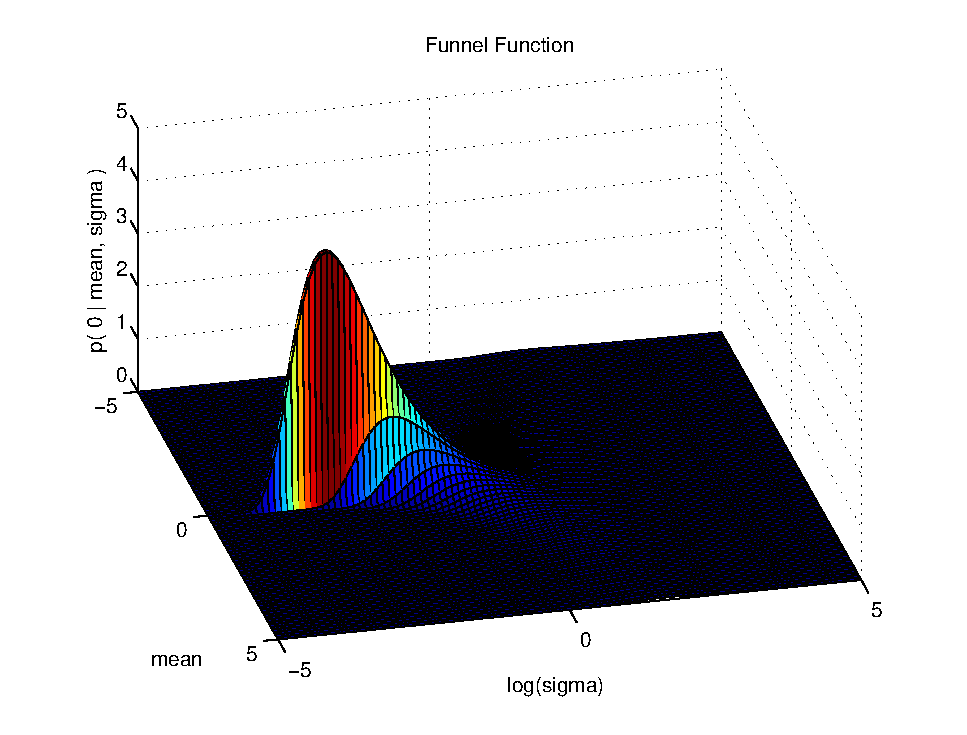
\includegraphics[width=0.45\textwidth]{figures/integrands/funnel.eps}
%\caption{Radford Neal's funnel problem in 2 dimensions.}
%\label{fig:funnel}
%\end{figure}

%\begin{minipage}[t][0.45\paperheight][t]{0.45\paperwidth}
%    % --- Automatically generated by latex_table.m ---
% Exported at 16-Feb-2012 13:24:18
\begin{table}[h!]
\caption{{\small
time taken (s)
}}
\label{tbl:time taken (s)}
\begin{center}
\begin{tabular}{l  r r r r r r r}
Integrand & \rotatebox{0}{ SMC }  & \rotatebox{0}{ AIS }  & \rotatebox{0}{ BMC AIS }  & \rotatebox{0}{ LBMC }  & \rotatebox{0}{ SBQ }  & \rotatebox{0}{ SBQ GPML }  & \rotatebox{0}{ BQ AIS }  \\ \midrule
simple & $\mathbf{0.023}$ & $1.306$ & $2.026$ & $1.251$ & $36.344$ & $12.158$ & $22.325$ \\
simple translated & $\mathbf{0.009}$ & $1.295$ & $1.948$ & $1.384$ & $ NaN$ & $ NaN$ & $23.192$ \\
simple scaled & $\mathbf{0.012}$ & $1.288$ & $1.897$ & $1.116$ & $37.762$ & $11.947$ & $21.611$ \\
easy 1d & $\mathbf{0.009}$ & $1.766$ & $2.064$ & $1.079$ & $45.821$ & $12.779$ & $ NaN$ \\
bumpy 1d & $\mathbf{0.007}$ & $1.126$ & $2.119$ & $1.144$ & $16.984$ & $26.335$ & $35.352$ \\
two spikes 1d & $\mathbf{0.016}$ & $2.781$ & $2.342$ & $1.888$ & $45.635$ & $ NaN$ & $45.693$ \\
two hills 1d & $\mathbf{0.020}$ & $2.781$ & $2.151$ & $1.091$ & $38.483$ & $11.402$ & $30.592$ \\
funnel 2d & $\mathbf{0.033}$ & $2.566$ & $2.241$ & $0.618$ & $67.442$ & $6.688$ & $9.770$ \\
friedman 3d & $\mathbf{0.371}$ & $12.441$ & $3.578$ & $0.447$ & $171.890$ & $7.807$ & $11.814$ \\
easy 4d & $\mathbf{0.010}$ & $1.924$ & $2.518$ & $0.666$ & $147.084$ & $10.071$ & $11.208$ \\
two spikes 4d & $\mathbf{0.012}$ & $2.997$ & $2.829$ & $ NaN$ & $ NaN$ & $ NaN$ & $ NaN$ \\
two hills 4d & $\mathbf{0.012}$ & $2.984$ & $2.321$ & $0.637$ & $219.580$ & $16.164$ & $11.057$ \\
friedman 7d & $\mathbf{0.356}$ & $11.618$ & $3.990$ & $4.756$ & $443.423$ & $57.409$ & $ NaN$ \\
\end{tabular}
\end{center}
\end{table}
% End automatically generated LaTeX

%\end{minipage}

%% --- Automatically generated by latex_table.m ---
% Exported at 11-Feb-2012 20:59:11
\begin{table}[h!]
\caption{{\small
neg log density of truth at 100 samples
}}
\label{tbl:neg log density of truth at 100 samples}
\begin{center}
\begin{tabular}{l  r r r r r r}
Integrand & \rotatebox{0}{ SMC }  & \rotatebox{0}{ AIS }  & \rotatebox{0}{ BMC }  & \rotatebox{0}{ SBQ }  & \rotatebox{0}{ SBQ GPML }  & \rotatebox{0}{ BQ GPML AIS }  \\ \midrule
simple test & $-1.186$ & $233.335$ & $\mathbf{-2.942}$ & $-2.237$ & $-0.999$ & $-1.915$ \\
simple test transformed & $-1.186$ & $233.335$ & $\mathbf{-2.942}$ & $ NaN$ & $-1.104$ & $-1.915$ \\
easy 1d & $0.627$ & $\mathbf{-2.198}$ & $-1.189$ & $-0.453$ & $-1.145$ & $-1.353$ \\
bumpy 1d & $\mathbf{-3.050}$ & $>$ 1000 & $3.163$ & $-2.043$ & $ NaN$ & $0.867$ \\
bumpy 1d exp & $\mathbf{-3.518}$ & $>$ 1000 & $0.731$ & $-2.424$ & $ NaN$ & $0.015$ \\
two spikes 1d & $2.970$ & $24.156$ & $1.386$ & $ NaN$ & $\mathbf{0.120}$ & $1.220$ \\
two hills 1d & $2.970$ & $24.156$ & $1.386$ & $ NaN$ & $\mathbf{0.120}$ & $1.220$ \\
funnel 2d & $12.439$ & $52.654$ & $\mathbf{0.493}$ & $ NaN$ & $ NaN$ & $0.782$ \\
friedman 3d & $\mathbf{ NaN}$ & $ NaN$ & $ NaN$ & $ NaN$ & $ NaN$ & $ NaN$ \\
easy 4d & $0.601$ & $44.220$ & $0.410$ & $ NaN$ & $ NaN$ & $\mathbf{0.328}$ \\
two spikes 4d & $\mathbf{5.977}$ & $153.904$ & $23.489$ & $ NaN$ & $ NaN$ & $13.897$ \\
two hills 4d & $2.741$ & $687.308$ & $21.552$ & $ NaN$ & $ NaN$ & $\mathbf{0.356}$ \\
friedman 7d & $\mathbf{ NaN}$ & $ NaN$ & $ NaN$ & $ NaN$ & $ NaN$ & $ NaN$ \\
\end{tabular}
\end{center}
\end{table}
% End automatically generated LaTeX

%% --- Automatically generated by latex_table.m ---
% Exported at 24-Feb-2012 15:01:01
\begin{table}[h!]
\caption{{\small
log squared error at 150 samples
}}
\label{tbl:log squared error at 150 samples}
\begin{center}
\begin{tabular}{l  r r r r r r r}
Integrand & \rotatebox{0}{ SMC }  & \rotatebox{0}{ AIS }  & \rotatebox{0}{ BMC }  & \rotatebox{0}{ BQ }  & \rotatebox{0}{ BQ* }  & \rotatebox{0}{ BBQ }  & \rotatebox{0}{ BBQ* }  \\ \midrule
simple & $-5.713$ & $-0.758$ & $-10.933$ & $-10.336$ & $-10.336$ & $-13.335$ & $\mathbf{-14.468}$ \\
bumpy 1d & $-4.859$ & $-6.866$ & $-3.286$ & $-3.466$ & $-3.466$ & $-2.594$ & $\mathbf{-10.106}$ \\
two spikes 1d & $-1.294$ & $\mathbf{-5.449}$ & $-0.821$ & $-0.574$ & $-0.574$ & $-1.724$ & $-3.628$ \\
two hills 1d & $-9.423$ & $-2.346$ & $-5.229$ & $-14.669$ & $-14.669$ & $\mathbf{-18.318}$ & $-18.317$ \\
funnel 2d & $-3.921$ & $-0.070$ & $-1.467$ & $-1.437$ & $-1.437$ & $-2.206$ & $\mathbf{-4.454}$ \\
easy 4d & $-6.665$ & $-4.655$ & $-4.073$ & $\mathbf{-6.785}$ & $-6.785$ & $-1.909$ & $-5.237$ \\
two spikes 4d & $-2.030$ & $3.664$ & $-3.540$ & $-2.275$ & $-2.275$ & $-2.322$ & $\mathbf{-4.772}$ \\
two hills 4d & $-0.707$ & $2.858$ & $-1.909$ & $-1.265$ & $-1.265$ & $-2.725$ & $\mathbf{-3.543}$ \\
real prawn 6d mean field & $\mathbf{-7.259}$ & $2.173$ & $-1.416$ & $-1.187$ & $-1.187$ & $2.084$ & $2.083$ \\
real prawn 6d markov & $\mathbf{-5.056}$ & $3.795$ & $3.000$ & $3.028$ & $3.028$ & $3.408$ & $3.412$ \\
real prawn 6d non-markov & $\mathbf{3.621}$ & $4.499$ & $3.710$ & $3.642$ & $3.642$ & $4.343$ & $4.346$ \\
\end{tabular}
\end{center}
\end{table}
% End automatically generated LaTeX


\begin{figure}
	\centering
	\setlength\fheight{4cm} 
	\setlength\fwidth{4cm}
	% This file was created by matlab2tikz v0.1.4.
% Copyright (c) 2008--2012, Nico Schlömer <nico.schloemer@gmail.com>
% All rights reserved.
% 
% 
% 
\begin{tikzpicture}

% defining custom colors
\definecolor{mycolor1}{rgb}{1,0.316227766016838,0.316227766016838}
\definecolor{mycolor2}{rgb}{0.316227766016838,1,0.316227766016838}
\definecolor{mycolor3}{rgb}{0.316227766016838,0.316227766016838,1}
\definecolor{mycolor4}{rgb}{0.632455532033676,0.632455532033676,0.316227766016838}
\definecolor{mycolor5}{rgb}{0.316227766016838,1,1}
\definecolor{mycolor6}{rgb}{0.948683298050514,0.316227766016838,0.948683298050514}


\begin{axis}[%
xmin=0, xmax=2,
ymin=0, ymax=2,
scale only axis,
width=\fwidth,
height=\fheight,
axis on top,
legend entries={SMC,AIS,BMC,SBQ,SBQ GPML,BQ GPML AIS,True value},
legend style={nodes=right}]
\end{axis}
\end{tikzpicture}

\end{figure}

\begin{figure}
	\centering
	\setlength\fheight{4cm} 
	\setlength\fwidth{4cm}
	% This file was created by matlab2tikz v0.1.4.
% Copyright (c) 2008--2012, Nico Schlömer <nico.schloemer@gmail.com>
% All rights reserved.
% 
% 
% 
\begin{tikzpicture}

% defining custom colors
\definecolor{mycolor1}{rgb}{1,0.1,0.1}
\definecolor{mycolor2}{rgb}{0.1,1,0.1}
\definecolor{mycolor3}{rgb}{0.1,0.1,1}
\definecolor{mycolor4}{rgb}{0.4,0.4,0.1}
\definecolor{mycolor5}{rgb}{0.1,1,1}
\definecolor{mycolor6}{rgb}{0.9,0.1,0.9}


\begin{semilogyaxis}[%
xmin=30, xmax=100,
xlabel={Number of samples},
ymin=1e-08, ymax=100,
yminorticks=true,
ylabel={Squared Distance to True Value},
scale only axis,
width=\fwidth,
height=\fheight,
title={easy 1d},
axis on top]
\addplot [
color=mycolor1,
solid,
line width=1.0pt
]
coordinates{
 (30,0.000230372751786821)(31,0.000297046687420698)(32,0.00237573105193247)(33,0.000870756447042093)(34,0.00339476090290883)(35,0.00738798688490439)(36,0.0130139487611276)(37,0.020006839952991)(38,0.0282622437338889)(39,0.0320930009236307)(40,0.0404657080528455)(41,0.0150240473765445)(42,0.00245830112126412)(43,0.00534527127048734)(44,0.000115533938143997)(45,0.00110098254665758)(46,0.000502380233788551)(47,2.27375800771392e-06)(48,0.00189830595963212)(49,0.000631306834763216)(50,2.49412114008338e-05)(51,0.00142146966495412)(52,0.000334315581200544)(53,0.00211093113998183)(54,0.000742711752985978)(55,0.000838781288676129)(56,0.00111422847591404)(57,0.000252135253668436)(58,0.00144984986751528)(59,0.00235981709929402)(60,0.00121427551253199)(61,0.000335521449438383)(62,0.00138540631682358)(63,0.000450318335535026)(64,0.00323245789183337)(65,0.00603779719089331)(66,0.0108034090583615)(67,0.00790558519694972)(68,0.0148756697698894)(69,0.0235827574033825)(70,0.0299285801789756)(71,0.0399571110171522)(72,0.0345612470528094)(73,0.0296229652276023)(74,0.0277966083522507)(75,0.0365744654232679)(76,0.0316837480498924)(77,0.0272009872741444)(78,0.0325555218373256)(79,0.0281339032979143)(80,0.0240724106994399)(81,0.0321927484018474)(82,0.0416466982287099)(83,0.0437757303330521)(84,0.0389093200258927)(85,0.0350933366167813)(86,0.0349603035027832)(87,0.0357405897083466)(88,0.0317542443228047)(89,0.0278565735353225)(90,0.0242517039375702)(91,0.020932231306752)(92,0.0178892455179196)(93,0.0151141866337706)(94,0.0130387244321351)(95,0.0187639695740051)(96,0.0204392243252047)(97,0.0226358772973077)(98,0.0282820394962359)(99,0.0249713563291721)(100,0.0266959403154322) 
};

\addplot [
color=mycolor2,
solid,
line width=1.0pt
]
coordinates{
 (30,0.596436236196016)(31,0.497326384668056)(32,0.412627391228598)(33,0.34025888900581)(34,0.278516522658938)(35,0.225959150054937)(36,0.202243514397932)(37,0.171282180116067)(38,0.19337358950346)(39,0.158188215603831)(40,0.541279716319922)(41,0.488968007636532)(42,0.424617305681433)(43,0.369143858165017)(44,0.319812894314883)(45,0.279545923200763)(46,0.243563951572507)(47,0.211435149176666)(48,0.179335749839804)(49,0.153102968186985)(50,0.128830477280461)(51,0.129721526770983)(52,0.130581201073703)(53,0.109563299615319)(54,0.099129853491371)(55,0.0887800258735989)(56,0.0737296008926354)(57,0.060531461332288)(58,0.0490352147463144)(59,0.0382817363931984)(60,0.0291503755223414)(61,0.0232536171698495)(62,0.018353931974481)(63,0.0133952596391319)(64,0.00874044248739668)(65,0.00523317240063309)(66,0.00299010102805719)(67,0.00123676451364297)(68,0.000240747518318772)(69,1.27161370700421e-05)(70,0.0873729058175499)(71,0.0824826896115387)(72,0.0861248711526042)(73,0.0927722228384807)(74,0.0908729441259075)(75,0.0890431771834566)(76,0.0872794432785116)(77,0.083933411492404)(78,0.0807360796942653)(79,0.0776794425157849)(80,0.0720300758162284)(81,0.0644152245466956)(82,0.0417967277900732)(83,0.0363345843067189)(84,0.0300463355514569)(85,0.0269771840625102)(86,0.0239813338191286)(87,0.021224600132611)(88,0.0167562823438974)(89,0.012898241613537)(90,0.00961332869787512)(91,0.00840403416082463)(92,0.00729965553337208)(93,0.00497404424427641)(94,0.00319596115742572)(95,0.0018417874016879)(96,0.000887196830547832)(97,0.000286502142544981)(98,2.3520049981494e-05)(99,5.02773160054575e-05)(100,0.000353148256708148) 
};

\addplot [
color=mycolor3,
solid,
line width=1.0pt
]
coordinates{
 (30,0.000103880647206628)(31,8.06591198793197e-05)(32,7.1685691242131e-05)(33,6.65221973763399e-05)(34,6.31739986629022e-05)(35,6.08296565444028e-05)(36,4.73833400113928e-05)(37,6.64150637046037e-05)(38,5.05899669997456e-05)(39,5.10352516541163e-05)(40,0.000284015189315978)(41,0.000285085868938255)(42,0.000275320736699448)(43,0.000278078251820838)(44,0.000280230940762707)(45,0.00027596943073216)(46,0.000272455096369162)(47,0.000269507510183559)(48,0.000266368606495862)(49,0.000280083244703477)(50,0.000284347981683757)(51,0.000284110272155085)(52,0.00028391381839282)(53,0.000284616758131412)(54,0.000284882049094361)(55,0.00028676890794686)(56,0.000286937959433023)(57,0.000287085135593955)(58,0.000287162338896649)(59,0.000281013097697759)(60,0.000275827895766814)(61,0.000271843621732921)(62,0.00027671207245924)(63,0.000279099763288545)(64,0.000272777237167413)(65,0.000271095524764021)(66,0.000272277740661878)(67,0.000272311139240834)(68,0.000268576611719484)(69,0.000265279894008902)(70,1.05186219065924e-06)(71,1.70455814718923e-08)(72,4.10824281885928e-08)(73,4.88879228289524e-08)(74,5.14970533415136e-08)(75,5.33635087410286e-08)(76,5.47607481884392e-08)(77,4.12030856929425e-08)(78,3.17701034406417e-08)(79,2.49784110747365e-08)(80,1.53870442104735e-07)(81,3.33516532046114e-07)(82,1.07570278186093e-06)(83,1.29606062284842e-06)(84,1.12624504686938e-06)(85,1.03819495718052e-06)(86,9.36619983753754e-07)(87,8.5069227369129e-07)(88,6.99914440663439e-07)(89,5.80155567115746e-07)(90,4.83904768673749e-07)(91,5.75459212800695e-07)(92,6.59799646126056e-07)(93,7.07823417051318e-07)(94,6.66551511766703e-07)(95,6.42006293924657e-07)(96,6.45050030924331e-07)(97,6.47810105029892e-07)(98,6.08908997087961e-07)(99,5.80841797784366e-07)(100,5.56714791537151e-07) 
};

\addplot [
color=mycolor4,
solid,
line width=1.0pt
]
coordinates{
 (30,6.71827018347208)(31,6.89347312264796)(32,7.06511717379667)(33,7.23336080589035)(34,7.39835189603822)(35,7.56022864471161)(36,7.71912037928052)(37,7.87514833279294)(38,8.02842624291207)(39,8.17906104267939)(40,5.32171000415946)(41,5.33481530760045)(42,5.34357961537645)(43,5.35174654627048)(44,5.35941479624089)(45,5.36656545099828)(46,5.37328593306092)(47,5.37964541855913)(48,5.38558321382669)(49,5.39113909410357)(50,5.3958629147579)(51,5.40083479592915)(52,5.40558571445033)(53,5.4100247524801)(54,5.41432703492478)(55,5.41842500427517)(56,5.42219804801152)(57,5.42582255227741)(58,5.42930944674151)(59,5.43269304707752)(60,5.43576251968577)(61,5.43883090029841)(62,5.44175108984825)(63,5.32730609602612)(64,5.32947834326858)(65,5.33140537093565)(66,5.33332977205351)(67,5.33512461298819)(68,5.3369533040182)(69,5.33855276512775)(70,5.34035551903846)(71,5.34186132510066)(72,5.34348316048681)(73,5.34483681435897)(74,5.34635369683066)(75,5.34758790589463)(76,5.34895857920538)(77,5.35013064234709)(78,5.35154005983262)(79,5.3525267000899)(80,5.35383947698495)(81,5.35478887898653)(82,5.35595710715786)(83,5.3567744956593)(84,5.35802009042609)(85,5.35872916032734)(86,5.35979111917365)(87,5.3605682330116)(88,5.36169314166884)(89,5.3623689504655)(90,5.36337594284992)(91,5.36399109792719)(92,5.36493310549562)(93,5.36549938745434)(94,5.36638241223407)(95,5.36695584217212)(96,5.36778240622827)(97,5.3682709850866)(98,5.36916177009518)(99,5.36951723408481)(100,5.37035260605019) 
};

\addplot [
color=mycolor5,
solid,
line width=1.0pt
]
coordinates{
 (30,5.88612661434799e-06)(31,5.66572595613712e-06)(32,6.14447135465207e-06)(33,5.94427042581199e-06)(34,6.4511271777847e-06)(35,7.06239267415294e-06)(36,7.34344864550081e-06)(37,7.34962312029186e-06)(38,7.49075093254774e-06)(39,7.37984732740989e-06)(40,7.37977449890474e-06)(41,7.2112855981099e-06)(42,7.20910048228378e-06)(43,7.134275126382e-06)(44,7.1292588828103e-06)(45,8.00484968548362e-06)(46,8.30192974621025e-06)(47,8.29738879083813e-06)(48,8.22717134763537e-06)(49,8.22134710417114e-06)(50,8.26367494318793e-06)(51,8.2592325415369e-06)(52,8.20572813881838e-06)(53,8.20091969013643e-06)(54,8.19684120366871e-06)(55,8.28688420755726e-06)(56,8.24448316469648e-06)(57,8.24051364466707e-06)(58,8.26437892855086e-06)(59,8.57540877293462e-06)(60,8.57197006583793e-06)(61,8.56895263782858e-06)(62,8.53262900069246e-06)(63,8.5295933819273e-06)(64,8.54443559213975e-06)(65,8.52209971431371e-06)(66,8.80350600075539e-06)(67,8.58166262898459e-06)(68,8.57937608283356e-06)(69,8.55416569512645e-06)(70,8.55190198622663e-06)(71,8.54986187598443e-06)(72,8.52866453678741e-06)(73,8.53814532514888e-06)(74,8.57266895523456e-06)(75,8.57069664187566e-06)(76,8.56889300321837e-06)(77,8.55069820055772e-06)(78,8.54895031400031e-06)(79,8.55592036065796e-06)(80,8.55432126702676e-06)(81,8.53858338291039e-06)(82,8.53703358547125e-06)(83,8.52567229756714e-06)(84,8.5243707985069e-06)(85,8.51183126438479e-06)(86,8.51056708089876e-06)(87,8.51570683682049e-06)(88,8.53412669329208e-06)(89,8.53295683426881e-06)(90,8.52186550454477e-06)(91,8.52073985606536e-06)(92,8.51967341581902e-06)(93,8.52372752127243e-06)(94,8.51387422538913e-06)(95,8.51285130698105e-06)(96,8.5118916222836e-06)(97,8.50309314523166e-06)(98,8.5021696158619e-06)(99,8.49701159884025e-06)(100,8.50021142697616e-06) 
};

\addplot [
color=mycolor6,
solid,
line width=1.0pt
]
coordinates{
 (30,0.000145739163307982)(31,0.00014831468069588)(32,0.000144093112206235)(33,0.000141625822152934)(34,0.000140004828908002)(35,0.000138857749825056)(36,8.52532146209903e-05)(37,7.92628675445e-05)(38,9.53282577894208e-05)(39,9.63669529319848e-05)(40,0.00134960667822393)(41,0.00134680913497267)(42,0.00136854408766632)(43,0.0013773640505149)(44,0.00138382155663823)(45,0.0014368623470837)(46,0.00147840507079048)(47,0.00151182737410321)(48,0.00156269570329953)(49,0.00186628248020599)(50,0.00192092753079824)(51,0.00193799230263561)(52,0.00200560742396369)(53,0.0020558151151629)(54,0.00219924566341558)(55,0.00217723822409065)(56,0.00217145137339494)(57,0.00215286213777132)(58,0.00213476881312014)(59,0.00187177020926658)(60,0.00196369200406033)(61,0.00206501810994325)(62,0.00229218276288917)(63,0.00251049908288703)(64,0.00249129541844772)(65,0.00247104679651697)(66,0.00241773080790437)(67,0.00243886347702086)(68,0.00238215372357939)(69,0.00234380890335451)(70,0.000945764664914174)(71,0.00103937640028663)(72,0.00113072594370314)(73,0.00119286295703679)(74,0.0012146326853806)(75,0.00120863241413656)(76,0.00119798528708272)(77,0.00111890228199717)(78,0.00105256987353346)(79,0.00102569299593514)(80,0.00104384928616805)(81,0.00112807692538742)(82,0.00125266775285161)(83,0.00131124542619765)(84,0.0013126031722376)(85,0.00130716090237763)(86,0.00130098650451132)(87,0.00129561095433513)(88,0.00129405997613507)(89,0.00128252552375633)(90,0.00127248935597362)(91,0.0012584918802823)(92,0.00124399597891212)(93,0.00117187687766632)(94,0.00117418746376299)(95,0.00117815134393718)(96,0.00117331586403476)(97,0.00117217984032967)(98,0.00116639525903504)(99,0.00116540540101895)(100,0.00116713748234355) 
};

\end{semilogyaxis}
\end{tikzpicture}

\end{figure}

%\begin{figure}
%	\centering
%	\setlength\fheight{4cm} 
%	\setlength\fwidth{4cm}
%	% This file was created by matlab2tikz v0.1.4.
% Copyright (c) 2008--2011, Nico Schlömer <nico.schloemer@gmail.com>
% All rights reserved.
% 
\begin{tikzpicture}

% defining custom colors
\definecolor{mycolor1}{rgb}{1,0.1,0.1}
\definecolor{mycolor2}{rgb}{0.1,1,0.1}
\definecolor{mycolor3}{rgb}{0.1,0.1,1}
\definecolor{mycolor4}{rgb}{0.4,0.4,0.1}


\begin{semilogyaxis}[%
scale only axis,
width=\fwidth,
height=\fheight,
xmin=0, xmax=250,
ymin=1e-07, ymax=1,
yminorticks=true,
xlabel={Number of samples},
ylabel={Squared Distance to True Value},
title={$\text{sanity hard }1d$},
axis on top]
\addplot [
color=mycolor1,
solid,
line width=1.0pt
]
coordinates{
 (10,5.74619e-05)(20,0.000247289)(30,3.59312e-05)(40,6.72275e-05)(50,1.23698e-06)(100,0.000127854)(150,3.21991e-05)(200,1.04579e-05)(250,4.72674e-07) 
};

\addplot [
color=mycolor2,
solid,
line width=1.0pt
]
coordinates{
 (10,4.79482e-05)(20,0.000256417)(30,2.53732e-07)(40,6.493e-05)(50,5.35818e-05)(100,2.02467e-05)(150,4.07626e-05)(200,3.20687e-06)(250,3.67676e-05) 
};

\addplot [
color=mycolor3,
solid,
line width=1.0pt
]
coordinates{
 (10,0.394168)(20,0.0659873)(30,0.0712942)(40,0.0541693)(50,0.128508)(100,0.000364344)(150,0.000451895)(200,0.00975937)(250,0.000520116) 
};

\addplot [
color=mycolor4,
solid,
line width=1.0pt
]
coordinates{
 (10,0.00809716)(20,0.0112574)(30,0.0105948)(40,0.00719612)(50,0.00798252)(100,0.00888599)(150,0.00521284)(200,0.00898904)(250,0.00888976) 
};

\end{semilogyaxis}
\end{tikzpicture}
 
%\end{figure}

%\begin{figure}
%	\centering
%	\setlength\fheight{4cm} 
%	\setlength\fwidth{4cm}
%	% This file was created by matlab2tikz v0.1.4.
% Copyright (c) 2008--2011, Nico Schlömer <nico.schloemer@gmail.com>
% All rights reserved.
% 
\begin{tikzpicture}

% defining custom colors
\definecolor{mycolor1}{rgb}{1,0.1,0.1}
\definecolor{mycolor2}{rgb}{1,0.316228,0.316228}
\definecolor{mycolor3}{rgb}{0.1,1,0.1}
\definecolor{mycolor4}{rgb}{0.316228,1,0.316228}
\definecolor{mycolor5}{rgb}{0.1,0.1,1}
\definecolor{mycolor6}{rgb}{0.316228,0.316228,1}
\definecolor{mycolor7}{rgb}{0.4,0.4,0.1}
\definecolor{mycolor8}{rgb}{0.632456,0.632456,0.316228}


\begin{axis}[%
scale only axis,
width=\fwidth,
height=\fheight,
xmin=0, xmax=250,
ymin=-3.5, ymax=1.5,
xlabel={Number of samples},
ylabel={log evidence},
title={$\text{sanity easy }1d$},
axis on top,
legend entries={SMC,AIS,BMC,SBQ,True value},
legend style={nodes=right}]
\addplot [fill=mycolor1,opacity=1.000000e-01,draw=none] coordinates{ (10,1.0244)(20,1.36828)(30,0.657109)(40,0.215982)(50,0.237312)(100,0.543573)(150,0.305464)(200,0.207231)(250,0.0462748)(250,-2.06841)(200,-2.15329)(150,-2.22352)(100,-2.37033)(50,-2.38086)(40,-2.77184)(30,-2.78028)(20,-2.929)(10,-2.97385)};
\addplot [
color=mycolor2,
solid,
line width=1.0pt
]
coordinates{
 (10,-0.974728)(20,-0.780361)(30,-1.06159)(40,-1.27793)(50,-1.07177)(100,-0.913377)(150,-0.959031)(200,-0.973028)(250,-1.01107) 
};

\addplot [fill=mycolor3,opacity=1.000000e-01,draw=none] coordinates{ (10,-2.46961)(20,-2.14007)(30,-1.94472)(40,-1.50437)(50,-1.88688)(100,-1.4404)(150,-0.941737)(200,-1.79939)(250,-1.85773)(250,-1.86992)(200,-1.81854)(150,-0.952519)(100,-1.46205)(50,-1.96002)(40,-1.57293)(30,-2.04657)(20,-2.33078)(10,-3.20995)};
\addplot [
color=mycolor4,
solid,
line width=1.0pt
]
coordinates{
 (10,-2.83978)(20,-2.23542)(30,-1.99565)(40,-1.53865)(50,-1.92345)(100,-1.45123)(150,-0.947128)(200,-1.80897)(250,-1.86383) 
};

\addplot [fill=mycolor5,opacity=1.000000e-01,draw=none] coordinates{ (10,-1.13096)(20,-1.07824)(30,-1.08875)(40,-1.08759)(50,-1.07114)(100,-1.08407)(150,-1.0845)(200,-1.08418)(250,-1.07325)(250,-1.07325)(200,-1.08418)(150,-1.0845)(100,-1.08407)(50,-1.07114)(40,-1.08759)(30,-1.08875)(20,-1.07824)(10,-1.13096)};
\addplot [
color=mycolor6,
solid,
line width=1.0pt
]
coordinates{
 (10,-1.13096)(20,-1.07824)(30,-1.08875)(40,-1.08759)(50,-1.07114)(100,-1.08407)(150,-1.0845)(200,-1.08418)(250,-1.07325) 
};

\addplot [fill=mycolor7,opacity=1.000000e-01,draw=none] coordinates{ (10,-1.31243)(20,-1.16884)(30,-1.06143)(40,-1.08024)(50,-1.07788)(100,-1.07686)(150,-1.07677)(200,-1.07681)(250,-1.07657)(250,-1.07657)(200,-1.07681)(150,-1.07677)(100,-1.07686)(50,-1.07788)(40,-1.08024)(30,-1.06143)(20,-1.16884)(10,-1.31243)};
\addplot [
color=mycolor8,
solid,
line width=1.0pt
]
coordinates{
 (10,-1.31243)(20,-1.16884)(30,-1.06143)(40,-1.08024)(50,-1.07788)(100,-1.07686)(150,-1.07677)(200,-1.07681)(250,-1.07657) 
};

\addplot [
color=black,
solid,
line width=1.0pt
]
coordinates{
 (10,-1.07677)(20,-1.07677)(30,-1.07677)(40,-1.07677)(50,-1.07677)(100,-1.07677)(150,-1.07677)(200,-1.07677)(250,-1.07677) 
};

\end{axis}
\end{tikzpicture}
 
%\end{figure}

\begin{figure}
	\centering
	\setlength\fheight{4cm} 
	\setlength\fwidth{4cm}
	% This file was created by matlab2tikz v0.1.4.
% Copyright (c) 2008--2012, Nico Schlömer <nico.schloemer@gmail.com>
% All rights reserved.
% 
% 
% 
\begin{tikzpicture}

% defining custom colors
\definecolor{mycolor1}{rgb}{1,0.1,0.1}
\definecolor{mycolor2}{rgb}{0.1,1,0.1}
\definecolor{mycolor3}{rgb}{0.1,0.1,1}
\definecolor{mycolor4}{rgb}{0.4,0.4,0.1}
\definecolor{mycolor5}{rgb}{0.1,1,1}
\definecolor{mycolor6}{rgb}{0.9,0.1,0.9}


\begin{axis}[%
xmin=30, xmax=100,
xlabel={Number of samples},
ymin=-1.84905882181668, ymax=0.132460526584802,
ylabel={log evidence},
axis lines=left,
scale only axis,
width=\fwidth,
height=\fheight,
title={easy 1d},
axis on top]
\addplot [fill=mycolor1,opacity=1.000000e-01,draw=none] coordinates{ (30,0.657108766065047)(31,0.571266761968604)(32,0.491359665199035)(33,0.475049053539778)(34,0.399267215892366)(35,0.327152894441738)(36,0.270566510977558)(37,0.218071609685913)(38,0.320565379230859)(39,0.275542261876489)(40,0.215981668104371)(41,0.275451596754609)(42,0.329501684019585)(43,0.318138065264759)(44,0.362170558203052)(45,0.313741894815762)(46,0.352262323576102)(47,0.301176479087694)(48,0.326450844890934)(49,0.280516168634261)(50,0.23731246137394)(51,0.254507261778838)(52,0.305379410276021)(53,0.316763141453984)(54,0.366363859522445)(55,0.348373283363205)(56,0.334004870323478)(57,0.292651969274678)(58,0.299385535983918)(59,0.293492747337001)(60,0.258657332619311)(61,0.253121502071302)(62,0.257744683582962)(63,0.351870182517919)(64,0.373563163510844)(65,0.379652006023384)(66,0.3918597004634)(67,0.360725416174019)(68,0.381077919664023)(69,0.400138837862572)(70,0.406403510431664)(71,0.420938580815935)(72,0.414064457273807)(73,0.42862396762966)(74,0.40786540992027)(75,0.420650319621817)(76,0.430249994312579)(77,0.428705149157874)(78,0.432280325122856)(79,0.403610463730584)(80,0.404315495921255)(81,0.418031132579846)(82,0.432317566241553)(83,0.42568068788989)(84,0.402024772862897)(85,0.377846102708914)(86,0.365788273381773)(87,0.356675725949816)(88,0.331717234857189)(89,0.309763915621076)(90,0.603711020496451)(91,0.593341232535275)(92,0.591208138833802)(93,0.589994646956422)(94,0.565949646744367)(95,0.577322080047709)(96,0.570968796008742)(97,0.566431999404637)(98,0.572984719419436)(99,0.549755409582145)(100,0.543572621629513)(100,-2.37032673120934)(99,-2.38724081050286)(98,-2.39017138018855)(97,-2.41905947078156)(96,-2.4385691220796)(95,-2.45689075748289)(94,-2.49110713507463)(93,-2.4976470668596)(92,-2.47723872701566)(91,-2.45751368045502)(90,-2.4457838051497)(89,-2.12949009907808)(88,-2.12885477885174)(87,-2.13210404744258)(86,-2.14536673814285)(85,-2.15671374753822)(84,-2.16104781935621)(83,-2.16075963472029)(82,-2.17769906900551)(81,-2.21271633407)(80,-2.24754172773184)(79,-2.22167913883144)(78,-2.22494930579565)(77,-2.25238266947062)(76,-2.22778336630207)(75,-2.19169324142272)(74,-2.22795106881813)(73,-2.23792945669116)(72,-2.19578330455898)(71,-2.17468503978092)(70,-2.21393789368793)(69,-2.24653722473687)(68,-2.29067816633177)(67,-2.33643065709177)(66,-2.33751275900063)(65,-2.37777743514378)(64,-2.41338570281507)(63,-2.46296072835533)(62,-2.33683454673625)(61,-2.3700189694242)(60,-2.34249637667463)(59,-2.34986880648611)(58,-2.37676370423618)(57,-2.41442639104122)(56,-2.42077670475375)(55,-2.44398179771358)(54,-2.46539033916048)(53,-2.37840535667023)(52,-2.42234276928961)(51,-2.33263445281742)(50,-2.38085618255074)(49,-2.38379648500808)(48,-2.39284369517481)(47,-2.45169263854381)(46,-2.46096659965574)(45,-2.53363596544342)(44,-2.53719985765866)(43,-2.61789274603381)(42,-2.58219615608026)(41,-2.67412879494643)(40,-2.77183542645068)(39,-2.78736460859199)(38,-2.81032489997893)(37,-2.65449464033406)(36,-2.65225585846287)(35,-2.6525916499702)(34,-2.66932832591273)(33,-2.68759817527577)(32,-2.74237456489872)(31,-2.75926880335693)(30,-2.78028465225081)};
\addplot [
color=mycolor1,
solid,
line width=1.0pt
]
coordinates{
 (30,-1.06158794309288)(31,-1.09400102069416)(32,-1.12550744984984)(33,-1.106274560868)(34,-1.13503055501018)(35,-1.16271937776423)(36,-1.19084467374266)(37,-1.21821151532407)(38,-1.24487976037403)(39,-1.25591117335775)(40,-1.27792687917315)(41,-1.19933859909591)(42,-1.12634723603034)(43,-1.14987734038452)(44,-1.0875146497278)(45,-1.10994703531383)(46,-1.05435213803982)(47,-1.07525807972806)(48,-1.03319642514194)(49,-1.05164015818691)(50,-1.0717718605884)(51,-1.03906359551929)(52,-1.0584816795068)(53,-1.03082110760812)(54,-1.04951323981902)(55,-1.04780425717519)(56,-1.04338591721514)(57,-1.06088721088327)(58,-1.03868908412613)(59,-1.02818802957455)(60,-1.04191952202766)(61,-1.05844873367645)(62,-1.03954493157665)(63,-1.0555452729187)(64,-1.01991126965211)(65,-0.999062714560199)(66,-0.972826529268615)(67,-0.987852620458876)(68,-0.954800123333875)(69,-0.923199193437148)(70,-0.903767191628134)(71,-0.876873229482494)(72,-0.890859423642587)(73,-0.90465274453075)(74,-0.910042829448932)(75,-0.885521460900451)(76,-0.898766685994745)(77,-0.911838760156373)(78,-0.896334490336399)(79,-0.90903433755043)(80,-0.921613115905291)(81,-0.897342600745076)(82,-0.87269075138198)(83,-0.867539473415198)(84,-0.879511523246655)(85,-0.889433822414653)(86,-0.889789232380537)(87,-0.887714160746383)(88,-0.898568771997274)(89,-0.909863091728501)(90,-0.921036392326627)(91,-0.932086223959872)(92,-0.943015294090928)(93,-0.953826209951589)(94,-0.962578744165133)(95,-0.93978433871759)(96,-0.933800163035427)(97,-0.926313735688461)(98,-0.908593330384555)(99,-0.918742700460355)(100,-0.913377054789911) 
};

\addplot [fill=mycolor2,opacity=1.000000e-01,draw=none] coordinates{ (30,-1.65625577243318)(31,-1.59796309178675)(32,-1.54190560605138)(33,-1.48947405687015)(34,-1.44029779978548)(35,-1.3940633812863)(36,-1.37524129262297)(37,-1.34621734420641)(38,-1.38561967059262)(39,-1.34909376320966)(40,-1.70131693615516)(41,-1.66882441101608)(42,-1.62577241401271)(43,-1.58400907633456)(44,-1.54444841805061)(45,-1.50999194881447)(46,-1.47752626705143)(47,-1.44647409860624)(48,-1.41289046992426)(49,-1.38274245532301)(50,-1.35276392246135)(51,-1.35737810258936)(52,-1.36160026542024)(53,-1.33661579095853)(54,-1.32209469024364)(55,-1.30754294744125)(56,-1.28369978241701)(57,-1.25974118053608)(58,-1.23664731149526)(59,-1.21238832246919)(60,-1.18876366193788)(61,-1.17170131879958)(62,-1.15620365229915)(63,-1.13805994643551)(64,-1.11721306235063)(65,-1.09715917308163)(66,-1.08054703063448)(67,-1.06230310663853)(68,-1.04372898545191)(69,-1.02564401120996)(70,-1.33107231761749)(71,-1.32430519259135)(72,-1.33209434076569)(73,-1.34421739589542)(74,-1.34221333909385)(75,-1.34012012715586)(76,-1.33806952888565)(77,-1.33326286316891)(78,-1.32852168024493)(79,-1.32389083650781)(80,-1.31440795607441)(81,-1.30056128591777)(82,-1.25035606898842)(83,-1.23707936541839)(84,-1.22040572743236)(85,-1.21172066896797)(86,-1.20294590219052)(87,-1.19435413025946)(88,-1.17883431165083)(89,-1.16330705301032)(90,-1.14812946537561)(91,-1.14213319322676)(92,-1.13643697292324)(93,-1.1222506593479)(94,-1.10855778447348)(95,-1.09526350942358)(96,-1.08245283922508)(97,-1.06991663367774)(98,-1.05815327024261)(99,-1.04654192093662)(100,-1.03515982895584)(100,-1.08078764904467)(99,-1.09280873579986)(98,-1.10507818112241)(97,-1.11746807119902)(96,-1.13065081631529)(95,-1.14410054837331)(94,-1.15803983718613)(93,-1.17233510598915)(92,-1.18797102679526)(91,-1.19474580212779)(90,-1.20149765885135)(89,-1.21736575510116)(88,-1.23358976406982)(87,-1.25055112726826)(86,-1.26030420892623)(85,-1.27030593935167)(84,-1.27980380583203)(83,-1.29768524610319)(82,-1.31206084833828)(81,-1.36057376180998)(80,-1.37589238930876)(79,-1.38706176017694)(78,-1.39329217709188)(77,-1.39969436548624)(76,-1.40632431770148)(75,-1.41021389768636)(74,-1.41422140936171)(73,-1.41848521928616)(72,-1.40837840035694)(71,-1.40362275840046)(70,-1.41363780433986)(69,-1.12075600672065)(68,-1.14083505244056)(67,-1.16156417569227)(66,-1.18234855839591)(65,-1.20105412158308)(64,-1.22329956150107)(63,-1.24694779405384)(62,-1.26828167273089)(61,-1.2868133727884)(60,-1.30623791563314)(59,-1.33245801608374)(58,-1.35976257290102)(57,-1.38585362293086)(56,-1.41289607788284)(55,-1.44190855357634)(54,-1.46113514144066)(53,-1.47892311301995)(52,-1.514652110293)(51,-1.51649134921177)(50,-1.51862728847119)(49,-1.55335698887711)(48,-1.58760252429901)(47,-1.62669941674919)(46,-1.66304966332326)(45,-1.70098205946923)(44,-1.74012358077433)(43,-1.78466708261595)(42,-1.83101286506936)(41,-1.88323249365202)(40,-1.92364930884959)(39,-1.59989583670928)(38,-1.64739756610159)(37,-1.63503963941607)(36,-1.67772051531495)(35,-1.71017178878216)(34,-1.76872744930954)(33,-1.83069218513183)(32,-1.89634794091425)(31,-1.96599629594662)(30,-2.04186187120018)};
\addplot [
color=mycolor2,
solid,
line width=1.0pt
]
coordinates{
 (30,-1.84905882181668)(31,-1.78197969386668)(32,-1.71912677348281)(33,-1.66008312100099)(34,-1.60451262454751)(35,-1.55211758503423)(36,-1.52648090396896)(37,-1.49062849181124)(38,-1.5165086183471)(39,-1.47449479995947)(40,-1.81248312250238)(41,-1.77602845233405)(42,-1.72839263954104)(43,-1.68433807947526)(44,-1.64228599941247)(45,-1.60548700414185)(46,-1.57028796518735)(47,-1.53658675767771)(48,-1.50024649711163)(49,-1.46804972210006)(50,-1.43569560546627)(51,-1.43693472590057)(52,-1.43812618785662)(53,-1.40776945198924)(54,-1.39161491584215)(55,-1.3747257505088)(56,-1.34829793014992)(57,-1.32279740173347)(58,-1.29820494219814)(59,-1.27242316927646)(60,-1.24750078878551)(61,-1.22925734579399)(62,-1.21224266251502)(63,-1.19250387024468)(64,-1.17025631192585)(65,-1.14910664733236)(66,-1.13144779451519)(67,-1.1119336411654)(68,-1.09228201894623)(69,-1.0732000089653)(70,-1.37235506097867)(71,-1.36396397549591)(72,-1.37023637056131)(73,-1.38135130759079)(74,-1.37821737422778)(75,-1.37516701242111)(76,-1.37219692329357)(77,-1.36647861432757)(78,-1.36090692866841)(79,-1.35547629834238)(80,-1.34515017269159)(81,-1.33056752386388)(82,-1.28120845866335)(83,-1.26738230576079)(84,-1.25010476663219)(85,-1.24101330415982)(86,-1.23162505555838)(87,-1.22245262876386)(88,-1.20621203786032)(89,-1.19033640405574)(90,-1.17481356211348)(91,-1.16843949767727)(92,-1.16220399985925)(93,-1.14729288266853)(94,-1.13329881082981)(95,-1.11968202889845)(96,-1.10655182777018)(97,-1.09369235243838)(98,-1.08161572568251)(99,-1.06967532836824)(100,-1.05797373900025) 
};

\addplot [fill=mycolor3,opacity=1.000000e-01,draw=none] coordinates{ (30,-0.765732203902483)(31,-0.766815169172755)(32,-0.767266505835219)(33,-0.767539150150542)(34,-0.767721549601385)(35,-0.767852159111971)(36,-0.783031611690488)(37,-0.784370297074462)(38,-0.783302047380718)(39,-0.783319914364951)(40,-0.825462938824626)(41,-0.825496055956417)(42,-0.825310250328844)(43,-0.825337533727401)(44,-0.825358910581023)(45,-0.825332871364606)(46,-0.825311237665808)(47,-0.825292977626306)(48,-0.825238012707065)(49,-0.825629166905685)(50,-0.825701195272863)(51,-0.825707047642926)(52,-0.825711743000839)(53,-0.825715052762282)(54,-0.825805226770563)(55,-0.825874104520459)(56,-0.825882761729747)(57,-0.825890327050513)(58,-0.825896658713818)(59,-0.825816178439272)(60,-0.825747641221692)(61,-0.825709991376477)(62,-0.826052338480935)(63,-0.826165548798886)(64,-0.826083086085748)(65,-0.826055790374605)(66,-0.826140621461998)(67,-0.826123033760967)(68,-0.826073562061209)(69,-0.826029568812685)(70,-0.832257338660602)(71,-0.833139520439248)(72,-0.833479512951498)(73,-0.833488720021087)(74,-0.833532865178601)(75,-0.833565092460266)(76,-0.833589621014655)(77,-0.833570432088051)(78,-0.833554792098234)(79,-0.833542212769316)(80,-0.833755890398476)(81,-0.833972626961489)(82,-0.834611963774947)(83,-0.834745571286092)(84,-0.834691980579108)(85,-0.834664752930202)(86,-0.834634425435528)(87,-0.834607482140399)(88,-0.834556443533498)(89,-0.834512044650188)(90,-0.834472945435605)(91,-0.834529662305941)(92,-0.834578298400316)(93,-0.834610509430777)(94,-0.834590070853987)(95,-0.834576449721344)(96,-0.834575236290298)(97,-0.834574110795926)(98,-0.834555331139308)(99,-0.834539034669255)(100,-0.834524731912301)(100,-1.32049949107312)(99,-1.32051718143076)(98,-1.32053727780776)(97,-1.32056757444783)(96,-1.32056301595448)(95,-1.32055800876009)(94,-1.32057473780302)(93,-1.32060409194902)(92,-1.32057820947175)(91,-1.32051947479999)(90,-1.32045027643321)(89,-1.32054327077727)(88,-1.32064872701755)(87,-1.32076913396317)(86,-1.32083311368312)(85,-1.32090504061261)(84,-1.3209624711381)(83,-1.32106327982238)(82,-1.32099431462802)(81,-1.32071434951619)(80,-1.320560592613)(79,-1.32030583514425)(78,-1.3203336486254)(77,-1.32036749665567)(76,-1.32041035548273)(75,-1.32042887507353)(74,-1.32045295232571)(73,-1.32048544881409)(72,-1.32045781995735)(71,-1.3201313188732)(70,-1.31922341121521)(69,-1.36007721815643)(68,-1.36023500880446)(67,-1.36041262917476)(66,-1.3603930192103)(65,-1.36040612513481)(64,-1.3604808092673)(63,-1.36077897879184)(62,-1.36074895234859)(61,-1.36079730679261)(60,-1.36100044878602)(59,-1.36124266849389)(58,-1.36152702936918)(57,-1.36152880452401)(56,-1.36152768116192)(55,-1.36152635982957)(54,-1.36148362668874)(53,-1.3615580793196)(52,-1.36151969925894)(51,-1.36153604954244)(50,-1.36155600294863)(49,-1.36137416445819)(48,-1.36093554958077)(47,-1.36107234670213)(46,-1.36123314633702)(45,-1.361423740487)(44,-1.36165324552265)(43,-1.36154577971248)(42,-1.36140728948174)(41,-1.36180487221426)(40,-1.36177451813611)(39,-1.38449983439498)(38,-1.38445523924945)(37,-1.38546074241838)(36,-1.38426745641764)(35,-1.37008112356509)(34,-1.36991397390653)(33,-1.36968057816595)(32,-1.36933196416373)(31,-1.36875470821109)(30,-1.36741536911682)};
\addplot [
color=mycolor3,
solid,
line width=1.0pt
]
coordinates{
 (30,-1.06657378650965)(31,-1.06778493869192)(32,-1.06829923499948)(33,-1.06860986415825)(34,-1.06881776175396)(35,-1.06896664133853)(36,-1.08364953405406)(37,-1.08491551974642)(38,-1.08387864331509)(39,-1.08390987437997)(40,-1.09361872848037)(41,-1.09365046408534)(42,-1.09335876990529)(43,-1.09344165671994)(44,-1.09350607805184)(45,-1.0933783059258)(46,-1.09327219200142)(47,-1.09318266216422)(48,-1.09308678114392)(49,-1.09350166568194)(50,-1.09362859911075)(51,-1.09362154859269)(52,-1.09361572112989)(53,-1.09363656604094)(54,-1.09364442672965)(55,-1.09370023217501)(56,-1.09370522144583)(57,-1.09370956578726)(58,-1.0937118440415)(59,-1.09352942346658)(60,-1.09337404500386)(61,-1.09325364908454)(62,-1.09340064541476)(63,-1.09347226379536)(64,-1.09328194767652)(65,-1.09323095775471)(66,-1.09326682033615)(67,-1.09326783146786)(68,-1.09315428543283)(69,-1.09305339348456)(70,-1.07574037493791)(71,-1.07663541965622)(72,-1.07696866645442)(73,-1.07698708441759)(74,-1.07699290875216)(75,-1.0769969837669)(76,-1.07699998824869)(77,-1.07696896437186)(78,-1.07694422036182)(79,-1.07692402395678)(80,-1.07715824150574)(81,-1.07734348823884)(82,-1.07780313920148)(83,-1.07790442555424)(84,-1.07782722585861)(85,-1.07778489677141)(86,-1.07773376955932)(87,-1.07768830805179)(88,-1.07760258527553)(89,-1.07752765771373)(90,-1.07746161093441)(91,-1.07752456855296)(92,-1.07757825393603)(93,-1.0776073006899)(94,-1.07758240432851)(95,-1.07756722924072)(96,-1.07756912612239)(97,-1.07757084262188)(98,-1.07754630447354)(99,-1.07752810805001)(100,-1.07751211149271) 
};

\addplot [fill=mycolor4,opacity=1.000000e-01,draw=none] coordinates{ (30,-0.549142456718844)(31,-0.555431443185168)(32,-0.48077772203579)(33,-0.477728660758969)(34,-0.476450025575338)(35,-0.475739942243721)(36,-0.60098372950744)(37,-0.474575221340278)(38,-0.474257847948198)(39,-0.474193196155872)(40,-0.480862074598413)(41,-0.480873864289753)(42,-0.480802660287692)(43,-0.611702296661524)(44,-0.60950463846612)(45,-0.609466152404924)(46,-0.609406204099849)(47,-0.609302621017409)(48,-0.609374107059625)(49,-0.609330299396422)(50,-0.609308960586152)(51,-0.537959682809872)(52,-0.533802717779643)(53,-0.533415414120189)(54,-0.532929160334292)(55,-0.532802894979472)(56,-0.532661938336866)(57,-0.532549619230063)(58,-0.532448244912834)(59,-0.532337096765779)(60,-0.612556344640328)(61,-0.612548968732381)(62,-0.612533029382497)(63,-0.578039981461649)(64,-0.575707440795331)(65,-0.575084264585292)(66,-0.574509086652595)(67,-0.574233557868533)(68,-0.573961178128952)(69,-0.573801466358624)(70,-0.573640998290951)(71,-0.573536359345209)(72,-0.573439804657973)(73,-0.573334829454094)(74,-0.57326025289352)(75,-0.573210224443895)(76,-0.573137299726818)(77,-0.573145480304403)(78,-0.573103022141122)(79,-0.573049095904142)(80,-0.572994560087014)(81,-0.625496297173036)(82,-0.625453749422357)(83,-0.573996429946318)(84,-0.573961576604919)(85,-0.573977041875162)(86,-0.573946725857618)(87,-0.573813803915814)(88,-0.573773482903393)(89,-0.626229278678009)(90,-0.626219190154009)(91,-0.626196251207195)(92,-0.626178177628448)(93,-0.626162034460743)(94,-0.626147989134507)(95,-0.626134841470313)(96,-0.626121703734365)(97,-0.626113598991679)(98,-0.626105443177201)(99,-0.626097369110864)(100,-0.626086724294306)(100,-1.62196471770366)(99,-1.62195463468488)(98,-1.62194657255559)(97,-1.62193850261648)(96,-1.62193063230569)(95,-1.62191811957756)(94,-1.62190585849654)(93,-1.62189343210191)(92,-1.6218787715581)(91,-1.62186179747573)(90,-1.62184208453596)(89,-1.62183214344482)(88,-1.62507699574879)(87,-1.62500135495233)(86,-1.62486283842687)(85,-1.62481126228668)(84,-1.62480560276917)(83,-1.62474642458404)(82,-1.62296454261062)(81,-1.62293037414776)(80,-1.62555202895094)(79,-1.62545032153626)(78,-1.62535473397607)(77,-1.62528418490316)(76,-1.62526491300251)(75,-1.62512872859732)(74,-1.62504594082116)(73,-1.62490767306716)(72,-1.6247147458297)(71,-1.62455121619712)(70,-1.62435896766373)(69,-1.62406112640815)(68,-1.62377375338603)(67,-1.62326236604443)(66,-1.622778355976)(65,-1.62167052846452)(64,-1.62060819859857)(63,-1.6158858090402)(62,-1.61138585189183)(61,-1.6113601158252)(60,-1.61137089285628)(59,-1.67707698195415)(58,-1.67676684635695)(57,-1.67660222483796)(56,-1.67639017754955)(55,-1.67608682867111)(54,-1.67588322092188)(53,-1.67466106497218)(52,-1.67393624089109)(51,-1.66663518429886)(50,-1.61633904447585)(49,-1.61631891557965)(48,-1.61627115141087)(47,-1.61643601167242)(46,-1.61632266407928)(45,-1.61625502321001)(44,-1.61621855709419)(43,-1.61388871995822)(42,-1.73521341018607)(41,-1.73509074111134)(40,-1.73503769167831)(39,-1.75041455508789)(38,-1.75012575563693)(37,-1.749575292022)(36,-1.64762955391839)(35,-1.74752004252885)(34,-1.74627561118024)(33,-1.74402001770159)(32,-1.73862036852706)(31,-1.71299265457071)(30,-1.71972824278096)};
\addplot [
color=mycolor4,
solid,
line width=1.0pt
]
coordinates{
 (30,-1.1344353497499)(31,-1.13421204887794)(32,-1.10969904528143)(33,-1.11087433923028)(34,-1.11136281837779)(35,-1.11162999238628)(36,-1.12430664171291)(37,-1.11207525668114)(38,-1.11219180179256)(39,-1.11230387562188)(40,-1.10794988313836)(41,-1.10798230270055)(42,-1.10800803523688)(43,-1.11279550830987)(44,-1.11286159778015)(45,-1.11286058780747)(46,-1.11286443408956)(47,-1.11286931634491)(48,-1.11282262923525)(49,-1.11282460748803)(50,-1.112824002531)(51,-1.10229743355436)(52,-1.10386947933537)(53,-1.10403823954619)(54,-1.10440619062809)(55,-1.10444486182529)(56,-1.10452605794321)(57,-1.10457592203401)(58,-1.10460754563489)(59,-1.10470703935996)(60,-1.1119636187483)(61,-1.11195454227879)(62,-1.11195944063716)(63,-1.09696289525093)(64,-1.09815781969695)(65,-1.0983773965249)(66,-1.0986437213143)(67,-1.09874796195648)(68,-1.09886746575749)(69,-1.09893129638338)(70,-1.09899998297734)(71,-1.09904378777117)(72,-1.09907727524384)(73,-1.09912125126062)(74,-1.09915309685734)(75,-1.09916947652061)(76,-1.09920110636466)(77,-1.09921483260378)(78,-1.09922887805859)(79,-1.0992497087202)(80,-1.09927329451898)(81,-1.1242133356604)(82,-1.12420914601649)(83,-1.09937142726518)(84,-1.09938358968704)(85,-1.09939415208092)(86,-1.09940478214224)(87,-1.09940757943407)(88,-1.09942523932609)(89,-1.12403071106142)(90,-1.12403063734498)(91,-1.12402902434146)(92,-1.12402847459328)(93,-1.12402773328133)(94,-1.12402692381552)(95,-1.12402648052394)(96,-1.12402616802003)(97,-1.12402605080408)(98,-1.1240260078664)(99,-1.12402600189787)(100,-1.12402572099898) 
};

\addplot [fill=mycolor5,opacity=1.000000e-01,draw=none] coordinates{ (30,-0.879278087479964)(31,-0.878739506488954)(32,-0.876289368542035)(33,-0.874772735314538)(34,-0.874428756591692)(35,-0.874707923030207)(36,-0.874689438381127)(37,-0.87438230838575)(38,-0.873712608500194)(39,-0.873430376989683)(40,-0.873778956540377)(41,-0.874002208454646)(42,-0.873917677101426)(43,-0.873657104162223)(44,-0.873427819798161)(45,-0.872934464800393)(46,-0.87492595017064)(47,-0.875148166395069)(48,-0.874939967497571)(49,-0.874858959394364)(50,-0.874665089985002)(51,-0.875000303833088)(52,-0.875329214178305)(53,-0.875524523129936)(54,-0.875343233275144)(55,-0.855306146176036)(56,-0.853397931310923)(57,-0.852234793141322)(58,-0.852192155553825)(59,-0.852050808481535)(60,-0.851728616781306)(61,-0.851594042956056)(62,-0.85176353438991)(63,-0.853320250423398)(64,-0.853197678667542)(65,-0.853441578294111)(66,-0.85339971150503)(67,-0.853281915658761)(68,-0.853442918507471)(69,-0.852702303865181)(70,-0.852591293799152)(71,-0.852304682584243)(72,-0.85247229290524)(73,-0.852364702616705)(74,-0.852312541389601)(75,-0.852441316946875)(76,-0.85233750493844)(77,-0.852560270319315)(78,-0.852462028976523)(79,-0.852222475723012)(80,-0.853278843918623)(81,-0.855958374249757)(82,-0.843075665059774)(83,-0.842512326331831)(84,-0.842502722963037)(85,-0.842647835177245)(86,-0.842566055929058)(87,-0.842047152903418)(88,-0.841969617227849)(89,-0.842161080442526)(90,-0.832185196392363)(91,-0.832047722000111)(92,-0.831983172868128)(93,-0.832126915901808)(94,-0.83212495531962)(95,-0.832258080406034)(96,-0.831893817891224)(97,-0.831830110756971)(98,-0.832935254499332)(99,-0.832875203453992)(100,-0.832995753694348)(100,-1.33951676247737)(99,-1.33964026108157)(98,-1.3395807690083)(97,-1.34080320005342)(96,-1.34074002140299)(95,-1.34034960320485)(94,-1.34048608804418)(93,-1.3404873042526)(92,-1.34063953103915)(91,-1.34057557632175)(90,-1.34066043183435)(89,-1.32978825246134)(88,-1.32998912330195)(87,-1.32991212813432)(86,-1.32935461465916)(85,-1.32927348683576)(84,-1.32942127263569)(83,-1.32941500860338)(82,-1.32906281051282)(81,-1.31504636724269)(80,-1.31794522762562)(79,-1.31910870688568)(78,-1.31884691155327)(77,-1.31874890051915)(76,-1.31898095809423)(75,-1.31887739196804)(74,-1.31900487724445)(73,-1.31895393026776)(72,-1.31884657854654)(71,-1.31901787561767)(70,-1.31870196962816)(69,-1.31859125968919)(68,-1.31779953730365)(67,-1.31796023057492)(66,-1.31784285759249)(65,-1.31780266631424)(64,-1.31805909887288)(63,-1.31793699159486)(62,-1.31965672728625)(61,-1.31982414013589)(60,-1.3196897460835)(59,-1.31933029252151)(58,-1.3191892022859)(57,-1.3191469295294)(56,-1.31791048369303)(55,-1.31613536386592)(54,-1.29437650992769)(53,-1.29419575895918)(52,-1.29438645682099)(51,-1.29473020351054)(50,-1.29507534960852)(49,-1.29488202248592)(48,-1.29480109085719)(47,-1.29459350401825)(46,-1.29480878943819)(45,-1.29700561878536)(44,-1.2964601990352)(43,-1.29623085899264)(42,-1.29597017695525)(41,-1.29588095901955)(40,-1.29608871363745)(39,-1.29645954718573)(38,-1.29617694975902)(37,-1.29542093307888)(36,-1.29511366866531)(35,-1.29508692501073)(34,-1.29534112131139)(33,-1.29499647141177)(32,-1.29305694882088)(31,-1.29049564377459)(30,-1.28994812142018)};
\addplot [
color=mycolor5,
solid,
line width=1.0pt
]
coordinates{
 (30,-1.08461310445007)(31,-1.08461757513177)(32,-1.08467315868146)(33,-1.08488460336315)(34,-1.08488493895154)(35,-1.08489742402047)(36,-1.08490155352322)(37,-1.08490162073231)(38,-1.08494477912961)(39,-1.08494496208771)(40,-1.08493383508891)(41,-1.0849415837371)(42,-1.08494392702834)(43,-1.08494398157743)(44,-1.08494400941668)(45,-1.08497004179288)(46,-1.08486736980441)(47,-1.08487083520666)(48,-1.08487052917738)(49,-1.08487049094014)(50,-1.08487021979676)(51,-1.08486525367182)(52,-1.08485783549965)(53,-1.08486014104456)(54,-1.08485987160142)(55,-1.08572075502098)(56,-1.08565420750198)(57,-1.08569086133536)(58,-1.08569067891986)(59,-1.08569055050152)(60,-1.0857091814324)(61,-1.08570909154597)(62,-1.08571013083808)(63,-1.08562862100913)(64,-1.08562838877021)(65,-1.08562212230418)(66,-1.08562128454876)(67,-1.08562107311684)(68,-1.08562122790556)(69,-1.08564678177719)(70,-1.08564663171365)(71,-1.08566127910096)(72,-1.08565943572589)(73,-1.08565931644223)(74,-1.08565870931702)(75,-1.08565935445746)(76,-1.08565923151633)(77,-1.08565458541923)(78,-1.0856544702649)(79,-1.08566559130435)(80,-1.08561203577212)(81,-1.08550237074622)(82,-1.0860692377863)(83,-1.0859636674676)(84,-1.08596199779936)(85,-1.0859606610065)(86,-1.08596033529411)(87,-1.08597964051887)(88,-1.0859793702649)(89,-1.08597466645194)(90,-1.08642281411336)(91,-1.08631164916093)(92,-1.08631135195364)(93,-1.0863071100772)(94,-1.0863055216819)(95,-1.08630384180544)(96,-1.0863169196471)(97,-1.0863166554052)(98,-1.08625801175382)(99,-1.08625773226778)(100,-1.08625625808586) 
};

\addplot [fill=mycolor6,opacity=1.000000e-01,draw=none] coordinates{ (30,-1.07542773168705)(31,-1.07547846083131)(32,-1.07560128912295)(33,-1.07566891716994)(34,-1.07571275464846)(35,-1.07574342431263)(36,-1.07398117884034)(37,-1.073822675526)(38,-1.07425988132899)(39,-1.07423661819573)(40,-1.07601404217423)(41,-1.07595203981481)(42,-1.07610486394229)(43,-1.07605106796971)(44,-1.07602029060427)(45,-1.07593755078798)(46,-1.0758711400949)(47,-1.07581991617886)(48,-1.07568298330639)(49,-1.0756639545748)(50,-1.0756201575673)(51,-1.07567242700962)(52,-1.07568522128627)(53,-1.07559908338396)(54,-1.07554263353638)(55,-1.07554203433503)(56,-1.07553211708338)(57,-1.0755412965553)(58,-1.07552987316492)(59,-1.07496939111768)(60,-1.07452247058369)(61,-1.07430756214182)(62,-1.07437619164072)(63,-1.07448091304434)(64,-1.07479212474819)(65,-1.07485292492592)(66,-1.07483831796069)(67,-1.07484065044961)(68,-1.07483960774707)(69,-1.07479971837591)(70,-0.858146897509747)(71,-0.869623642278613)(72,-0.873272258964573)(73,-0.871912521334761)(74,-0.869169758771364)(75,-0.867216633386937)(76,-0.865742769905005)(77,-0.865082051244508)(78,-0.864536655874126)(79,-0.864079134034247)(80,-0.866510280484034)(81,-0.868121963358237)(82,-0.88157864571997)(83,-0.88254201383022)(84,-0.881673969362642)(85,-0.881210849761667)(86,-0.880652003783761)(87,-0.880167742399721)(88,-0.879475352760379)(89,-0.878855130053637)(90,-0.878295096599287)(91,-0.879194260585214)(92,-0.879953023455756)(93,-0.879100419667545)(94,-0.878695578827816)(95,-0.878399381382054)(96,-0.878347463942452)(97,-0.87828765330583)(98,-0.87818190639701)(99,-0.878075331532214)(100,-0.87797575769881)(100,-1.2896556931648)(99,-1.28957668255397)(98,-1.28949369404423)(97,-1.28942839652819)(96,-1.28935456279743)(95,-1.28928786716421)(94,-1.28897486830288)(93,-1.28855497369906)(92,-1.2877433962947)(91,-1.28856947116054)(90,-1.28954881503324)(89,-1.28904329516941)(88,-1.28848515392647)(87,-1.28786409916379)(86,-1.28734430562839)(85,-1.28674509776164)(84,-1.286231046082)(83,-1.28537692522384)(82,-1.28660863779189)(81,-1.30089866834795)(80,-1.30289483921862)(79,-1.30553284611149)(78,-1.30509824111125)(77,-1.30458144702262)(76,-1.30395815557337)(75,-1.30248739889623)(74,-1.3005383211434)(73,-1.29780034287424)(72,-1.29648119222073)(71,-1.30036204519587)(70,-1.3130664435351)(69,-1.07479994139607)(68,-1.07483983076723)(67,-1.07484087346977)(66,-1.07483854098085)(65,-1.07485314794608)(64,-1.07479234776835)(63,-1.07448112795194)(62,-1.07437640654832)(61,-1.07430777704942)(60,-1.0745226854913)(59,-1.07496960602528)(58,-1.07553008807252)(57,-1.0755415114629)(56,-1.07553233199098)(55,-1.07554224924263)(54,-1.07554284844399)(53,-1.07559929829156)(52,-1.07568543619388)(51,-1.07567264191723)(50,-1.07562037247491)(49,-1.07566416948241)(48,-1.07568319821399)(47,-1.07582013108646)(46,-1.07587135500251)(45,-1.07593776569558)(44,-1.07602050551188)(43,-1.07605128287731)(42,-1.07610507884989)(41,-1.07595225472241)(40,-1.07601425708183)(39,-1.07423684121589)(38,-1.07426010434915)(37,-1.07382289854616)(36,-1.0739814018605)(35,-1.07574364733279)(34,-1.07571297766862)(33,-1.0756691401901)(32,-1.07560151214311)(31,-1.07547868385147)(30,-1.07542794659466)};
\addplot [
color=mycolor6,
solid,
line width=1.0pt
]
coordinates{
 (30,-1.07542783914086)(31,-1.07547857234139)(32,-1.07560140063303)(33,-1.07566902868002)(34,-1.07571286615854)(35,-1.07574353582271)(36,-1.07398129035042)(37,-1.07382278703608)(38,-1.07425999283907)(39,-1.07423672970581)(40,-1.07601414962803)(41,-1.07595214726861)(42,-1.07610497139609)(43,-1.07605117542351)(44,-1.07602039805808)(45,-1.07593765824178)(46,-1.0758712475487)(47,-1.07582002363266)(48,-1.07568309076019)(49,-1.0756640620286)(50,-1.0756202650211)(51,-1.07567253446343)(52,-1.07568532874007)(53,-1.07559919083776)(54,-1.07554274099018)(55,-1.07554214178883)(56,-1.07553222453718)(57,-1.0755414040091)(58,-1.07552998061872)(59,-1.07496949857148)(60,-1.07452257803749)(61,-1.07430766959562)(62,-1.07437629909452)(63,-1.07448102049814)(64,-1.07479223625827)(65,-1.074853036436)(66,-1.07483842947077)(67,-1.07484076195969)(68,-1.07483971925715)(69,-1.07479982988599)(70,-1.08560667052242)(71,-1.08499284373724)(72,-1.08487672559265)(73,-1.0848564321045)(74,-1.08485403995738)(75,-1.08485201614158)(76,-1.08485046273919)(77,-1.08483174913356)(78,-1.08481744849269)(79,-1.08480599007287)(80,-1.08470255985133)(81,-1.08451031585309)(82,-1.08409364175593)(83,-1.08395946952703)(84,-1.08395250772232)(85,-1.08397797376165)(86,-1.08399815470607)(87,-1.08401592078175)(88,-1.08398025334342)(89,-1.08394921261152)(90,-1.08392195581626)(91,-1.08388186587288)(92,-1.08384820987523)(93,-1.0838276966833)(94,-1.08383522356535)(95,-1.08384362427313)(96,-1.08385101336994)(97,-1.08385802491701)(98,-1.08383780022062)(99,-1.08382600704309)(100,-1.08381572543181) 
};

\addplot [
color=black,
solid,
line width=1.0pt
]
coordinates{
 (30,-1.07676597826832)(31,-1.07676597826832)(32,-1.07676597826832)(33,-1.07676597826832)(34,-1.07676597826832)(35,-1.07676597826832)(36,-1.07676597826832)(37,-1.07676597826832)(38,-1.07676597826832)(39,-1.07676597826832)(40,-1.07676597826832)(41,-1.07676597826832)(42,-1.07676597826832)(43,-1.07676597826832)(44,-1.07676597826832)(45,-1.07676597826832)(46,-1.07676597826832)(47,-1.07676597826832)(48,-1.07676597826832)(49,-1.07676597826832)(50,-1.07676597826832)(51,-1.07676597826832)(52,-1.07676597826832)(53,-1.07676597826832)(54,-1.07676597826832)(55,-1.07676597826832)(56,-1.07676597826832)(57,-1.07676597826832)(58,-1.07676597826832)(59,-1.07676597826832)(60,-1.07676597826832)(61,-1.07676597826832)(62,-1.07676597826832)(63,-1.07676597826832)(64,-1.07676597826832)(65,-1.07676597826832)(66,-1.07676597826832)(67,-1.07676597826832)(68,-1.07676597826832)(69,-1.07676597826832)(70,-1.07676597826832)(71,-1.07676597826832)(72,-1.07676597826832)(73,-1.07676597826832)(74,-1.07676597826832)(75,-1.07676597826832)(76,-1.07676597826832)(77,-1.07676597826832)(78,-1.07676597826832)(79,-1.07676597826832)(80,-1.07676597826832)(81,-1.07676597826832)(82,-1.07676597826832)(83,-1.07676597826832)(84,-1.07676597826832)(85,-1.07676597826832)(86,-1.07676597826832)(87,-1.07676597826832)(88,-1.07676597826832)(89,-1.07676597826832)(90,-1.07676597826832)(91,-1.07676597826832)(92,-1.07676597826832)(93,-1.07676597826832)(94,-1.07676597826832)(95,-1.07676597826832)(96,-1.07676597826832)(97,-1.07676597826832)(98,-1.07676597826832)(99,-1.07676597826832)(100,-1.07676597826832) 
};

\end{axis}
\end{tikzpicture}

\end{figure}

\section{Discussion}

Adjusting the number of candidate points allows one to trade off between computational speed and number of samples required.

While we used an active learning scheme in this paper, Bayesian Quadrature can be used on samples generated by any method.

\paragraph{Future Work}There are many ways to improve the GP model used to model likelihood functions.  First and foremost, the Gaussian kernel used in this paper has very weak generalization abilities.  Allowing a richer class of kernels will allow the GP model to shrink its posterior much more quickly.  For example, log-likelihood functions typically take the form of a sum of many terms, each depending only on a small number of variables.  This prior information could easily be incorporated into the GP, presumably allowing the SBQ algorithm to form concentrated posterior distributions over high-dimensional likelihoods.

The methods developed here can be applied without modification to discrete domains.

\section{Conclusions}

 In this paper, we have made several advances to the BMC method.  We have also demonstrated the many advantages of model-based integration over standard MCMC: a natural stopping criterion, an estimate of uncertainty in our integral, and the ability to use active learning to select our samples rather than monte carlo methods.

MCMC is an extremely widely used method, and advances in MCMC allow modelers [such as...] to use richer model classes and to be more confident in their model evaluations.  While we do not expect model-based integration approaches to be a better choice in every instance, we expect that this family of approaches will one day be seen as a standard alternative to MCMC.

\section*{Acknowledgements}

\bibliography{bub}
\bibliographystyle{icml2012}

\end{document} 


